\documentclass[twoside]{book}

% Packages required by doxygen
\usepackage{fixltx2e}
\usepackage{calc}
\usepackage{doxygen}
\usepackage[export]{adjustbox} % also loads graphicx
\usepackage{graphicx}
\usepackage[utf8]{inputenc}
\usepackage{makeidx}
\usepackage{multicol}
\usepackage{multirow}
\PassOptionsToPackage{warn}{textcomp}
\usepackage{textcomp}
\usepackage[nointegrals]{wasysym}
\usepackage[table]{xcolor}

% Font selection
\usepackage[T1]{fontenc}
\usepackage[scaled=.90]{helvet}
\usepackage{courier}
\usepackage{amssymb}
\usepackage{sectsty}
\renewcommand{\familydefault}{\sfdefault}
\allsectionsfont{%
  \fontseries{bc}\selectfont%
  \color{darkgray}%
}
\renewcommand{\DoxyLabelFont}{%
  \fontseries{bc}\selectfont%
  \color{darkgray}%
}
\newcommand{\+}{\discretionary{\mbox{\scriptsize$\hookleftarrow$}}{}{}}

% Page & text layout
\usepackage{geometry}
\geometry{%
  a4paper,%
  top=2.5cm,%
  bottom=2.5cm,%
  left=2.5cm,%
  right=2.5cm%
}
\tolerance=750
\hfuzz=15pt
\hbadness=750
\setlength{\emergencystretch}{15pt}
\setlength{\parindent}{0cm}
\setlength{\parskip}{3ex plus 2ex minus 2ex}
\makeatletter
\renewcommand{\paragraph}{%
  \@startsection{paragraph}{4}{0ex}{-1.0ex}{1.0ex}{%
    \normalfont\normalsize\bfseries\SS@parafont%
  }%
}
\renewcommand{\subparagraph}{%
  \@startsection{subparagraph}{5}{0ex}{-1.0ex}{1.0ex}{%
    \normalfont\normalsize\bfseries\SS@subparafont%
  }%
}
\makeatother

% Headers & footers
\usepackage{fancyhdr}
\pagestyle{fancyplain}
\fancyhead[LE]{\fancyplain{}{\bfseries\thepage}}
\fancyhead[CE]{\fancyplain{}{}}
\fancyhead[RE]{\fancyplain{}{\bfseries\leftmark}}
\fancyhead[LO]{\fancyplain{}{\bfseries\rightmark}}
\fancyhead[CO]{\fancyplain{}{}}
\fancyhead[RO]{\fancyplain{}{\bfseries\thepage}}
\fancyfoot[LE]{\fancyplain{}{}}
\fancyfoot[CE]{\fancyplain{}{}}
\fancyfoot[RE]{\fancyplain{}{\bfseries\scriptsize Generated by Doxygen }}
\fancyfoot[LO]{\fancyplain{}{\bfseries\scriptsize Generated by Doxygen }}
\fancyfoot[CO]{\fancyplain{}{}}
\fancyfoot[RO]{\fancyplain{}{}}
\renewcommand{\footrulewidth}{0.4pt}
\renewcommand{\chaptermark}[1]{%
  \markboth{#1}{}%
}
\renewcommand{\sectionmark}[1]{%
  \markright{\thesection\ #1}%
}

% Indices & bibliography
\usepackage{natbib}
\usepackage[titles]{tocloft}
\setcounter{tocdepth}{3}
\setcounter{secnumdepth}{5}
\makeindex

% Hyperlinks (required, but should be loaded last)
\usepackage{ifpdf}
\ifpdf
  \usepackage[pdftex,pagebackref=true]{hyperref}
\else
  \usepackage[ps2pdf,pagebackref=true]{hyperref}
\fi
\hypersetup{%
  colorlinks=true,%
  linkcolor=blue,%
  citecolor=blue,%
  unicode%
}

% Custom commands
\newcommand{\clearemptydoublepage}{%
  \newpage{\pagestyle{empty}\cleardoublepage}%
}

\usepackage{caption}
\captionsetup{labelsep=space,justification=centering,font={bf},singlelinecheck=off,skip=4pt,position=top}

%===== C O N T E N T S =====

\begin{document}

% Titlepage & ToC
\hypersetup{pageanchor=false,
             bookmarksnumbered=true,
             pdfencoding=unicode
            }
\pagenumbering{alph}
\begin{titlepage}
\vspace*{7cm}
\begin{center}%
{\Large My Project }\\
\vspace*{1cm}
{\large Generated by Doxygen 1.8.13}\\
\end{center}
\end{titlepage}
\clearemptydoublepage
\pagenumbering{roman}
\tableofcontents
\clearemptydoublepage
\pagenumbering{arabic}
\hypersetup{pageanchor=true}

%--- Begin generated contents ---
\chapter{Data Structure Index}
\section{Data Structures}
Here are the data structures with brief descriptions\+:\begin{DoxyCompactList}
\item\contentsline{section}{\hyperlink{struct_r_e_a_d_e_r___a_t_r___atr}{R\+E\+A\+D\+E\+R\+\_\+\+A\+T\+R\+\_\+\+Atr} }{\pageref{struct_r_e_a_d_e_r___a_t_r___atr}}{}
\item\contentsline{section}{\hyperlink{struct_r_e_a_d_e_r___a_t_r___protocol_specific_bytes}{R\+E\+A\+D\+E\+R\+\_\+\+A\+T\+R\+\_\+\+Protocol\+Specific\+Bytes} }{\pageref{struct_r_e_a_d_e_r___a_t_r___protocol_specific_bytes}}{}
\item\contentsline{section}{\hyperlink{struct_r_e_a_d_e_r___t_p_d_u___command}{R\+E\+A\+D\+E\+R\+\_\+\+T\+P\+D\+U\+\_\+\+Command} }{\pageref{struct_r_e_a_d_e_r___t_p_d_u___command}}{}
\item\contentsline{section}{\hyperlink{struct_r_e_a_d_e_r___t_p_d_u___data_field}{R\+E\+A\+D\+E\+R\+\_\+\+T\+P\+D\+U\+\_\+\+Data\+Field} }{\pageref{struct_r_e_a_d_e_r___t_p_d_u___data_field}}{}
\item\contentsline{section}{\hyperlink{struct_r_e_a_d_e_r___t_p_d_u___header}{R\+E\+A\+D\+E\+R\+\_\+\+T\+P\+D\+U\+\_\+\+Header} }{\pageref{struct_r_e_a_d_e_r___t_p_d_u___header}}{}
\end{DoxyCompactList}

\chapter{File Index}
\section{File List}
Here is a list of all files with brief descriptions\+:\begin{DoxyCompactList}
\item\contentsline{section}{\hyperlink{main_8h}{main.\+h} }{\pageref{main_8h}}{}
\item\contentsline{section}{\hyperlink{reader_8h}{reader.\+h} }{\pageref{reader_8h}}{}
\item\contentsline{section}{\hyperlink{reader__apdu_8h}{reader\+\_\+apdu.\+h} }{\pageref{reader__apdu_8h}}{}
\item\contentsline{section}{\hyperlink{reader__atr_8h}{reader\+\_\+atr.\+h} }{\pageref{reader__atr_8h}}{}
\item\contentsline{section}{\hyperlink{reader__hal_8h}{reader\+\_\+hal.\+h} \\*Prototypes de la couche d\textquotesingle{}abstraction }{\pageref{reader__hal_8h}}{}
\item\contentsline{section}{\hyperlink{reader__periph_8h}{reader\+\_\+periph.\+h} }{\pageref{reader__periph_8h}}{}
\item\contentsline{section}{\hyperlink{reader__pps_8h}{reader\+\_\+pps.\+h} }{\pageref{reader__pps_8h}}{}
\item\contentsline{section}{\hyperlink{reader__tpdu_8h}{reader\+\_\+tpdu.\+h} }{\pageref{reader__tpdu_8h}}{}
\item\contentsline{section}{\hyperlink{reader__utils_8h}{reader\+\_\+utils.\+h} }{\pageref{reader__utils_8h}}{}
\item\contentsline{section}{\hyperlink{stm32f4xx__hal__conf_8h}{stm32f4xx\+\_\+hal\+\_\+conf.\+h} }{\pageref{stm32f4xx__hal__conf_8h}}{}
\item\contentsline{section}{\hyperlink{stm32f4xx__it_8h}{stm32f4xx\+\_\+it.\+h} }{\pageref{stm32f4xx__it_8h}}{}
\end{DoxyCompactList}

\chapter{Data Structure Documentation}
\hypertarget{struct_r_e_a_d_e_r___a_t_r___atr}{}\section{R\+E\+A\+D\+E\+R\+\_\+\+A\+T\+R\+\_\+\+Atr Struct Reference}
\label{struct_r_e_a_d_e_r___a_t_r___atr}\index{R\+E\+A\+D\+E\+R\+\_\+\+A\+T\+R\+\_\+\+Atr@{R\+E\+A\+D\+E\+R\+\_\+\+A\+T\+R\+\_\+\+Atr}}


{\ttfamily \#include $<$reader\+\_\+atr.\+h$>$}



Collaboration diagram for R\+E\+A\+D\+E\+R\+\_\+\+A\+T\+R\+\_\+\+Atr\+:
\nopagebreak
\begin{figure}[H]
\begin{center}
\leavevmode
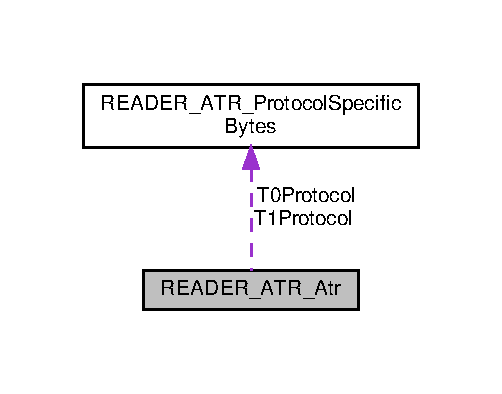
\includegraphics[width=241pt]{struct_r_e_a_d_e_r___a_t_r___atr__coll__graph}
\end{center}
\end{figure}
\subsection*{Data Fields}
\begin{DoxyCompactItemize}
\item 
uint32\+\_\+t \hyperlink{struct_r_e_a_d_e_r___a_t_r___atr_a4b9462052eea4404479658f230fa1c44}{Fi}
\item 
uint32\+\_\+t \hyperlink{struct_r_e_a_d_e_r___a_t_r___atr_aaf651c30f03f8f1e13a9485bffce801e}{Di}
\item 
uint32\+\_\+t \hyperlink{struct_r_e_a_d_e_r___a_t_r___atr_aad51bc4d2b761f55851ccd39a180ba58}{f\+Max}
\item 
uint8\+\_\+t \hyperlink{struct_r_e_a_d_e_r___a_t_r___atr_a77200420e0e4a3db85d736b7a0b91f64}{N}
\item 
\hyperlink{reader__atr_8h_a88b93dcccf6f332cf9a8a08100706e7f}{R\+E\+A\+D\+E\+R\+\_\+\+A\+T\+R\+\_\+\+Clock\+Stop\+Indicator} \hyperlink{struct_r_e_a_d_e_r___a_t_r___atr_a6ff1a13065a4f65bf3d92b693f828547}{clock\+Stop\+Indicator}
\item 
\hyperlink{reader__atr_8h_a59d38a6964b5cbc4d02b4569618e648b}{R\+E\+A\+D\+E\+R\+\_\+\+A\+T\+R\+\_\+\+Class\+Indicator} \hyperlink{struct_r_e_a_d_e_r___a_t_r___atr_a1aff6df1a1c438920c34249aa797896a}{class\+Indicator}
\item 
\hyperlink{reader__atr_8h_abefacd0599f2700370b31a1fae95caaf}{R\+E\+A\+D\+E\+R\+\_\+\+A\+T\+R\+\_\+\+Use\+Of\+S\+PU} \hyperlink{struct_r_e_a_d_e_r___a_t_r___atr_a7d23fda1eb2b5cd25709f6152299f944}{use\+Of\+S\+PU}
\item 
\hyperlink{reader__atr_8h_a193a4a51751968ed8d31224726c2b967}{R\+E\+A\+D\+E\+R\+\_\+\+A\+T\+R\+\_\+\+Encoding\+Conv} \hyperlink{struct_r_e_a_d_e_r___a_t_r___atr_a8b520c86d8fd45cf1ab80a917b22f8ba}{encoding\+Conv}
\item 
\hyperlink{struct_r_e_a_d_e_r___a_t_r___protocol_specific_bytes}{R\+E\+A\+D\+E\+R\+\_\+\+A\+T\+R\+\_\+\+Protocol\+Specific\+Bytes} \hyperlink{struct_r_e_a_d_e_r___a_t_r___atr_a701db7ee03dbfdfda068a8d01e3c5439}{T0\+Protocol}
\item 
\hyperlink{struct_r_e_a_d_e_r___a_t_r___protocol_specific_bytes}{R\+E\+A\+D\+E\+R\+\_\+\+A\+T\+R\+\_\+\+Protocol\+Specific\+Bytes} \hyperlink{struct_r_e_a_d_e_r___a_t_r___atr_a85a0512d06623db91c50d80ebee541f4}{T1\+Protocol}
\item 
uint32\+\_\+t \hyperlink{struct_r_e_a_d_e_r___a_t_r___atr_a847561bce07d061a0b82d34baf7d20d2}{K}
\item 
uint8\+\_\+t \hyperlink{struct_r_e_a_d_e_r___a_t_r___atr_a728edc393bb3b7e3853c5a5aaf019683}{hist\+Bytes} \mbox{[}\hyperlink{reader__atr_8h_a109a98f6497fb49ae8a3d26693628fa7}{R\+E\+A\+D\+E\+R\+\_\+\+A\+T\+R\+\_\+\+M\+A\+X\+\_\+\+H\+I\+S\+T\+\_\+\+B\+Y\+T\+ES}\mbox{]}
\end{DoxyCompactItemize}


\subsection{Field Documentation}
\mbox{\Hypertarget{struct_r_e_a_d_e_r___a_t_r___atr_a1aff6df1a1c438920c34249aa797896a}\label{struct_r_e_a_d_e_r___a_t_r___atr_a1aff6df1a1c438920c34249aa797896a}} 
\index{R\+E\+A\+D\+E\+R\+\_\+\+A\+T\+R\+\_\+\+Atr@{R\+E\+A\+D\+E\+R\+\_\+\+A\+T\+R\+\_\+\+Atr}!class\+Indicator@{class\+Indicator}}
\index{class\+Indicator@{class\+Indicator}!R\+E\+A\+D\+E\+R\+\_\+\+A\+T\+R\+\_\+\+Atr@{R\+E\+A\+D\+E\+R\+\_\+\+A\+T\+R\+\_\+\+Atr}}
\subsubsection{\texorpdfstring{class\+Indicator}{classIndicator}}
{\footnotesize\ttfamily \hyperlink{reader__atr_8h_a59d38a6964b5cbc4d02b4569618e648b}{R\+E\+A\+D\+E\+R\+\_\+\+A\+T\+R\+\_\+\+Class\+Indicator} class\+Indicator}

\mbox{\Hypertarget{struct_r_e_a_d_e_r___a_t_r___atr_a6ff1a13065a4f65bf3d92b693f828547}\label{struct_r_e_a_d_e_r___a_t_r___atr_a6ff1a13065a4f65bf3d92b693f828547}} 
\index{R\+E\+A\+D\+E\+R\+\_\+\+A\+T\+R\+\_\+\+Atr@{R\+E\+A\+D\+E\+R\+\_\+\+A\+T\+R\+\_\+\+Atr}!clock\+Stop\+Indicator@{clock\+Stop\+Indicator}}
\index{clock\+Stop\+Indicator@{clock\+Stop\+Indicator}!R\+E\+A\+D\+E\+R\+\_\+\+A\+T\+R\+\_\+\+Atr@{R\+E\+A\+D\+E\+R\+\_\+\+A\+T\+R\+\_\+\+Atr}}
\subsubsection{\texorpdfstring{clock\+Stop\+Indicator}{clockStopIndicator}}
{\footnotesize\ttfamily \hyperlink{reader__atr_8h_a88b93dcccf6f332cf9a8a08100706e7f}{R\+E\+A\+D\+E\+R\+\_\+\+A\+T\+R\+\_\+\+Clock\+Stop\+Indicator} clock\+Stop\+Indicator}

\mbox{\Hypertarget{struct_r_e_a_d_e_r___a_t_r___atr_aaf651c30f03f8f1e13a9485bffce801e}\label{struct_r_e_a_d_e_r___a_t_r___atr_aaf651c30f03f8f1e13a9485bffce801e}} 
\index{R\+E\+A\+D\+E\+R\+\_\+\+A\+T\+R\+\_\+\+Atr@{R\+E\+A\+D\+E\+R\+\_\+\+A\+T\+R\+\_\+\+Atr}!Di@{Di}}
\index{Di@{Di}!R\+E\+A\+D\+E\+R\+\_\+\+A\+T\+R\+\_\+\+Atr@{R\+E\+A\+D\+E\+R\+\_\+\+A\+T\+R\+\_\+\+Atr}}
\subsubsection{\texorpdfstring{Di}{Di}}
{\footnotesize\ttfamily uint32\+\_\+t Di}

\mbox{\Hypertarget{struct_r_e_a_d_e_r___a_t_r___atr_a8b520c86d8fd45cf1ab80a917b22f8ba}\label{struct_r_e_a_d_e_r___a_t_r___atr_a8b520c86d8fd45cf1ab80a917b22f8ba}} 
\index{R\+E\+A\+D\+E\+R\+\_\+\+A\+T\+R\+\_\+\+Atr@{R\+E\+A\+D\+E\+R\+\_\+\+A\+T\+R\+\_\+\+Atr}!encoding\+Conv@{encoding\+Conv}}
\index{encoding\+Conv@{encoding\+Conv}!R\+E\+A\+D\+E\+R\+\_\+\+A\+T\+R\+\_\+\+Atr@{R\+E\+A\+D\+E\+R\+\_\+\+A\+T\+R\+\_\+\+Atr}}
\subsubsection{\texorpdfstring{encoding\+Conv}{encodingConv}}
{\footnotesize\ttfamily \hyperlink{reader__atr_8h_a193a4a51751968ed8d31224726c2b967}{R\+E\+A\+D\+E\+R\+\_\+\+A\+T\+R\+\_\+\+Encoding\+Conv} encoding\+Conv}

\mbox{\Hypertarget{struct_r_e_a_d_e_r___a_t_r___atr_a4b9462052eea4404479658f230fa1c44}\label{struct_r_e_a_d_e_r___a_t_r___atr_a4b9462052eea4404479658f230fa1c44}} 
\index{R\+E\+A\+D\+E\+R\+\_\+\+A\+T\+R\+\_\+\+Atr@{R\+E\+A\+D\+E\+R\+\_\+\+A\+T\+R\+\_\+\+Atr}!Fi@{Fi}}
\index{Fi@{Fi}!R\+E\+A\+D\+E\+R\+\_\+\+A\+T\+R\+\_\+\+Atr@{R\+E\+A\+D\+E\+R\+\_\+\+A\+T\+R\+\_\+\+Atr}}
\subsubsection{\texorpdfstring{Fi}{Fi}}
{\footnotesize\ttfamily uint32\+\_\+t Fi}

\mbox{\Hypertarget{struct_r_e_a_d_e_r___a_t_r___atr_aad51bc4d2b761f55851ccd39a180ba58}\label{struct_r_e_a_d_e_r___a_t_r___atr_aad51bc4d2b761f55851ccd39a180ba58}} 
\index{R\+E\+A\+D\+E\+R\+\_\+\+A\+T\+R\+\_\+\+Atr@{R\+E\+A\+D\+E\+R\+\_\+\+A\+T\+R\+\_\+\+Atr}!f\+Max@{f\+Max}}
\index{f\+Max@{f\+Max}!R\+E\+A\+D\+E\+R\+\_\+\+A\+T\+R\+\_\+\+Atr@{R\+E\+A\+D\+E\+R\+\_\+\+A\+T\+R\+\_\+\+Atr}}
\subsubsection{\texorpdfstring{f\+Max}{fMax}}
{\footnotesize\ttfamily uint32\+\_\+t f\+Max}

\mbox{\Hypertarget{struct_r_e_a_d_e_r___a_t_r___atr_a728edc393bb3b7e3853c5a5aaf019683}\label{struct_r_e_a_d_e_r___a_t_r___atr_a728edc393bb3b7e3853c5a5aaf019683}} 
\index{R\+E\+A\+D\+E\+R\+\_\+\+A\+T\+R\+\_\+\+Atr@{R\+E\+A\+D\+E\+R\+\_\+\+A\+T\+R\+\_\+\+Atr}!hist\+Bytes@{hist\+Bytes}}
\index{hist\+Bytes@{hist\+Bytes}!R\+E\+A\+D\+E\+R\+\_\+\+A\+T\+R\+\_\+\+Atr@{R\+E\+A\+D\+E\+R\+\_\+\+A\+T\+R\+\_\+\+Atr}}
\subsubsection{\texorpdfstring{hist\+Bytes}{histBytes}}
{\footnotesize\ttfamily uint8\+\_\+t hist\+Bytes\mbox{[}\hyperlink{reader__atr_8h_a109a98f6497fb49ae8a3d26693628fa7}{R\+E\+A\+D\+E\+R\+\_\+\+A\+T\+R\+\_\+\+M\+A\+X\+\_\+\+H\+I\+S\+T\+\_\+\+B\+Y\+T\+ES}\mbox{]}}

\mbox{\Hypertarget{struct_r_e_a_d_e_r___a_t_r___atr_a847561bce07d061a0b82d34baf7d20d2}\label{struct_r_e_a_d_e_r___a_t_r___atr_a847561bce07d061a0b82d34baf7d20d2}} 
\index{R\+E\+A\+D\+E\+R\+\_\+\+A\+T\+R\+\_\+\+Atr@{R\+E\+A\+D\+E\+R\+\_\+\+A\+T\+R\+\_\+\+Atr}!K@{K}}
\index{K@{K}!R\+E\+A\+D\+E\+R\+\_\+\+A\+T\+R\+\_\+\+Atr@{R\+E\+A\+D\+E\+R\+\_\+\+A\+T\+R\+\_\+\+Atr}}
\subsubsection{\texorpdfstring{K}{K}}
{\footnotesize\ttfamily uint32\+\_\+t K}

\mbox{\Hypertarget{struct_r_e_a_d_e_r___a_t_r___atr_a77200420e0e4a3db85d736b7a0b91f64}\label{struct_r_e_a_d_e_r___a_t_r___atr_a77200420e0e4a3db85d736b7a0b91f64}} 
\index{R\+E\+A\+D\+E\+R\+\_\+\+A\+T\+R\+\_\+\+Atr@{R\+E\+A\+D\+E\+R\+\_\+\+A\+T\+R\+\_\+\+Atr}!N@{N}}
\index{N@{N}!R\+E\+A\+D\+E\+R\+\_\+\+A\+T\+R\+\_\+\+Atr@{R\+E\+A\+D\+E\+R\+\_\+\+A\+T\+R\+\_\+\+Atr}}
\subsubsection{\texorpdfstring{N}{N}}
{\footnotesize\ttfamily uint8\+\_\+t N}

\mbox{\Hypertarget{struct_r_e_a_d_e_r___a_t_r___atr_a701db7ee03dbfdfda068a8d01e3c5439}\label{struct_r_e_a_d_e_r___a_t_r___atr_a701db7ee03dbfdfda068a8d01e3c5439}} 
\index{R\+E\+A\+D\+E\+R\+\_\+\+A\+T\+R\+\_\+\+Atr@{R\+E\+A\+D\+E\+R\+\_\+\+A\+T\+R\+\_\+\+Atr}!T0\+Protocol@{T0\+Protocol}}
\index{T0\+Protocol@{T0\+Protocol}!R\+E\+A\+D\+E\+R\+\_\+\+A\+T\+R\+\_\+\+Atr@{R\+E\+A\+D\+E\+R\+\_\+\+A\+T\+R\+\_\+\+Atr}}
\subsubsection{\texorpdfstring{T0\+Protocol}{T0Protocol}}
{\footnotesize\ttfamily \hyperlink{struct_r_e_a_d_e_r___a_t_r___protocol_specific_bytes}{R\+E\+A\+D\+E\+R\+\_\+\+A\+T\+R\+\_\+\+Protocol\+Specific\+Bytes} T0\+Protocol}

\mbox{\Hypertarget{struct_r_e_a_d_e_r___a_t_r___atr_a85a0512d06623db91c50d80ebee541f4}\label{struct_r_e_a_d_e_r___a_t_r___atr_a85a0512d06623db91c50d80ebee541f4}} 
\index{R\+E\+A\+D\+E\+R\+\_\+\+A\+T\+R\+\_\+\+Atr@{R\+E\+A\+D\+E\+R\+\_\+\+A\+T\+R\+\_\+\+Atr}!T1\+Protocol@{T1\+Protocol}}
\index{T1\+Protocol@{T1\+Protocol}!R\+E\+A\+D\+E\+R\+\_\+\+A\+T\+R\+\_\+\+Atr@{R\+E\+A\+D\+E\+R\+\_\+\+A\+T\+R\+\_\+\+Atr}}
\subsubsection{\texorpdfstring{T1\+Protocol}{T1Protocol}}
{\footnotesize\ttfamily \hyperlink{struct_r_e_a_d_e_r___a_t_r___protocol_specific_bytes}{R\+E\+A\+D\+E\+R\+\_\+\+A\+T\+R\+\_\+\+Protocol\+Specific\+Bytes} T1\+Protocol}

\mbox{\Hypertarget{struct_r_e_a_d_e_r___a_t_r___atr_a7d23fda1eb2b5cd25709f6152299f944}\label{struct_r_e_a_d_e_r___a_t_r___atr_a7d23fda1eb2b5cd25709f6152299f944}} 
\index{R\+E\+A\+D\+E\+R\+\_\+\+A\+T\+R\+\_\+\+Atr@{R\+E\+A\+D\+E\+R\+\_\+\+A\+T\+R\+\_\+\+Atr}!use\+Of\+S\+PU@{use\+Of\+S\+PU}}
\index{use\+Of\+S\+PU@{use\+Of\+S\+PU}!R\+E\+A\+D\+E\+R\+\_\+\+A\+T\+R\+\_\+\+Atr@{R\+E\+A\+D\+E\+R\+\_\+\+A\+T\+R\+\_\+\+Atr}}
\subsubsection{\texorpdfstring{use\+Of\+S\+PU}{useOfSPU}}
{\footnotesize\ttfamily \hyperlink{reader__atr_8h_abefacd0599f2700370b31a1fae95caaf}{R\+E\+A\+D\+E\+R\+\_\+\+A\+T\+R\+\_\+\+Use\+Of\+S\+PU} use\+Of\+S\+PU}



The documentation for this struct was generated from the following file\+:\begin{DoxyCompactItemize}
\item 
\hyperlink{reader__atr_8h}{reader\+\_\+atr.\+h}\end{DoxyCompactItemize}

\hypertarget{struct_r_e_a_d_e_r___a_t_r___protocol_specific_bytes}{}\section{R\+E\+A\+D\+E\+R\+\_\+\+A\+T\+R\+\_\+\+Protocol\+Specific\+Bytes Struct Reference}
\label{struct_r_e_a_d_e_r___a_t_r___protocol_specific_bytes}\index{R\+E\+A\+D\+E\+R\+\_\+\+A\+T\+R\+\_\+\+Protocol\+Specific\+Bytes@{R\+E\+A\+D\+E\+R\+\_\+\+A\+T\+R\+\_\+\+Protocol\+Specific\+Bytes}}


{\ttfamily \#include $<$reader\+\_\+atr.\+h$>$}

\subsection*{Data Fields}
\begin{DoxyCompactItemize}
\item 
uint8\+\_\+t \hyperlink{struct_r_e_a_d_e_r___a_t_r___protocol_specific_bytes_a3bb85da59a5096e1b450cbce54733478}{T\+A\+Bytes\+Count}
\item 
uint8\+\_\+t \hyperlink{struct_r_e_a_d_e_r___a_t_r___protocol_specific_bytes_a1994caa40b881fecd6d791f727055a6c}{T\+B\+Bytes\+Count}
\item 
uint8\+\_\+t \hyperlink{struct_r_e_a_d_e_r___a_t_r___protocol_specific_bytes_ab9bb2af6efe5aae109843efabe3a204f}{T\+C\+Bytes\+Count}
\item 
uint8\+\_\+t \hyperlink{struct_r_e_a_d_e_r___a_t_r___protocol_specific_bytes_ad7b5edf79261941307ee7545b6cd88c0}{T\+A\+Bytes} \mbox{[}\hyperlink{reader__atr_8h_ab72f8cd7d1234d9173796c516f94671f}{R\+E\+A\+D\+E\+R\+\_\+\+A\+T\+R\+\_\+\+M\+A\+X\+\_\+\+S\+P\+E\+C\+I\+F\+I\+C\+\_\+\+B\+Y\+T\+ES}\mbox{]}
\item 
uint8\+\_\+t \hyperlink{struct_r_e_a_d_e_r___a_t_r___protocol_specific_bytes_a7f1c1c4eb03d88718b259e4c046139e3}{T\+B\+Bytes} \mbox{[}\hyperlink{reader__atr_8h_ab72f8cd7d1234d9173796c516f94671f}{R\+E\+A\+D\+E\+R\+\_\+\+A\+T\+R\+\_\+\+M\+A\+X\+\_\+\+S\+P\+E\+C\+I\+F\+I\+C\+\_\+\+B\+Y\+T\+ES}\mbox{]}
\item 
uint8\+\_\+t \hyperlink{struct_r_e_a_d_e_r___a_t_r___protocol_specific_bytes_a920fd664683dd872638a69afea315fc4}{T\+C\+Bytes} \mbox{[}\hyperlink{reader__atr_8h_ab72f8cd7d1234d9173796c516f94671f}{R\+E\+A\+D\+E\+R\+\_\+\+A\+T\+R\+\_\+\+M\+A\+X\+\_\+\+S\+P\+E\+C\+I\+F\+I\+C\+\_\+\+B\+Y\+T\+ES}\mbox{]}
\end{DoxyCompactItemize}


\subsection{Field Documentation}
\mbox{\Hypertarget{struct_r_e_a_d_e_r___a_t_r___protocol_specific_bytes_ad7b5edf79261941307ee7545b6cd88c0}\label{struct_r_e_a_d_e_r___a_t_r___protocol_specific_bytes_ad7b5edf79261941307ee7545b6cd88c0}} 
\index{R\+E\+A\+D\+E\+R\+\_\+\+A\+T\+R\+\_\+\+Protocol\+Specific\+Bytes@{R\+E\+A\+D\+E\+R\+\_\+\+A\+T\+R\+\_\+\+Protocol\+Specific\+Bytes}!T\+A\+Bytes@{T\+A\+Bytes}}
\index{T\+A\+Bytes@{T\+A\+Bytes}!R\+E\+A\+D\+E\+R\+\_\+\+A\+T\+R\+\_\+\+Protocol\+Specific\+Bytes@{R\+E\+A\+D\+E\+R\+\_\+\+A\+T\+R\+\_\+\+Protocol\+Specific\+Bytes}}
\subsubsection{\texorpdfstring{T\+A\+Bytes}{TABytes}}
{\footnotesize\ttfamily uint8\+\_\+t T\+A\+Bytes\mbox{[}\hyperlink{reader__atr_8h_ab72f8cd7d1234d9173796c516f94671f}{R\+E\+A\+D\+E\+R\+\_\+\+A\+T\+R\+\_\+\+M\+A\+X\+\_\+\+S\+P\+E\+C\+I\+F\+I\+C\+\_\+\+B\+Y\+T\+ES}\mbox{]}}

\mbox{\Hypertarget{struct_r_e_a_d_e_r___a_t_r___protocol_specific_bytes_a3bb85da59a5096e1b450cbce54733478}\label{struct_r_e_a_d_e_r___a_t_r___protocol_specific_bytes_a3bb85da59a5096e1b450cbce54733478}} 
\index{R\+E\+A\+D\+E\+R\+\_\+\+A\+T\+R\+\_\+\+Protocol\+Specific\+Bytes@{R\+E\+A\+D\+E\+R\+\_\+\+A\+T\+R\+\_\+\+Protocol\+Specific\+Bytes}!T\+A\+Bytes\+Count@{T\+A\+Bytes\+Count}}
\index{T\+A\+Bytes\+Count@{T\+A\+Bytes\+Count}!R\+E\+A\+D\+E\+R\+\_\+\+A\+T\+R\+\_\+\+Protocol\+Specific\+Bytes@{R\+E\+A\+D\+E\+R\+\_\+\+A\+T\+R\+\_\+\+Protocol\+Specific\+Bytes}}
\subsubsection{\texorpdfstring{T\+A\+Bytes\+Count}{TABytesCount}}
{\footnotesize\ttfamily uint8\+\_\+t T\+A\+Bytes\+Count}

\mbox{\Hypertarget{struct_r_e_a_d_e_r___a_t_r___protocol_specific_bytes_a7f1c1c4eb03d88718b259e4c046139e3}\label{struct_r_e_a_d_e_r___a_t_r___protocol_specific_bytes_a7f1c1c4eb03d88718b259e4c046139e3}} 
\index{R\+E\+A\+D\+E\+R\+\_\+\+A\+T\+R\+\_\+\+Protocol\+Specific\+Bytes@{R\+E\+A\+D\+E\+R\+\_\+\+A\+T\+R\+\_\+\+Protocol\+Specific\+Bytes}!T\+B\+Bytes@{T\+B\+Bytes}}
\index{T\+B\+Bytes@{T\+B\+Bytes}!R\+E\+A\+D\+E\+R\+\_\+\+A\+T\+R\+\_\+\+Protocol\+Specific\+Bytes@{R\+E\+A\+D\+E\+R\+\_\+\+A\+T\+R\+\_\+\+Protocol\+Specific\+Bytes}}
\subsubsection{\texorpdfstring{T\+B\+Bytes}{TBBytes}}
{\footnotesize\ttfamily uint8\+\_\+t T\+B\+Bytes\mbox{[}\hyperlink{reader__atr_8h_ab72f8cd7d1234d9173796c516f94671f}{R\+E\+A\+D\+E\+R\+\_\+\+A\+T\+R\+\_\+\+M\+A\+X\+\_\+\+S\+P\+E\+C\+I\+F\+I\+C\+\_\+\+B\+Y\+T\+ES}\mbox{]}}

\mbox{\Hypertarget{struct_r_e_a_d_e_r___a_t_r___protocol_specific_bytes_a1994caa40b881fecd6d791f727055a6c}\label{struct_r_e_a_d_e_r___a_t_r___protocol_specific_bytes_a1994caa40b881fecd6d791f727055a6c}} 
\index{R\+E\+A\+D\+E\+R\+\_\+\+A\+T\+R\+\_\+\+Protocol\+Specific\+Bytes@{R\+E\+A\+D\+E\+R\+\_\+\+A\+T\+R\+\_\+\+Protocol\+Specific\+Bytes}!T\+B\+Bytes\+Count@{T\+B\+Bytes\+Count}}
\index{T\+B\+Bytes\+Count@{T\+B\+Bytes\+Count}!R\+E\+A\+D\+E\+R\+\_\+\+A\+T\+R\+\_\+\+Protocol\+Specific\+Bytes@{R\+E\+A\+D\+E\+R\+\_\+\+A\+T\+R\+\_\+\+Protocol\+Specific\+Bytes}}
\subsubsection{\texorpdfstring{T\+B\+Bytes\+Count}{TBBytesCount}}
{\footnotesize\ttfamily uint8\+\_\+t T\+B\+Bytes\+Count}

\mbox{\Hypertarget{struct_r_e_a_d_e_r___a_t_r___protocol_specific_bytes_a920fd664683dd872638a69afea315fc4}\label{struct_r_e_a_d_e_r___a_t_r___protocol_specific_bytes_a920fd664683dd872638a69afea315fc4}} 
\index{R\+E\+A\+D\+E\+R\+\_\+\+A\+T\+R\+\_\+\+Protocol\+Specific\+Bytes@{R\+E\+A\+D\+E\+R\+\_\+\+A\+T\+R\+\_\+\+Protocol\+Specific\+Bytes}!T\+C\+Bytes@{T\+C\+Bytes}}
\index{T\+C\+Bytes@{T\+C\+Bytes}!R\+E\+A\+D\+E\+R\+\_\+\+A\+T\+R\+\_\+\+Protocol\+Specific\+Bytes@{R\+E\+A\+D\+E\+R\+\_\+\+A\+T\+R\+\_\+\+Protocol\+Specific\+Bytes}}
\subsubsection{\texorpdfstring{T\+C\+Bytes}{TCBytes}}
{\footnotesize\ttfamily uint8\+\_\+t T\+C\+Bytes\mbox{[}\hyperlink{reader__atr_8h_ab72f8cd7d1234d9173796c516f94671f}{R\+E\+A\+D\+E\+R\+\_\+\+A\+T\+R\+\_\+\+M\+A\+X\+\_\+\+S\+P\+E\+C\+I\+F\+I\+C\+\_\+\+B\+Y\+T\+ES}\mbox{]}}

\mbox{\Hypertarget{struct_r_e_a_d_e_r___a_t_r___protocol_specific_bytes_ab9bb2af6efe5aae109843efabe3a204f}\label{struct_r_e_a_d_e_r___a_t_r___protocol_specific_bytes_ab9bb2af6efe5aae109843efabe3a204f}} 
\index{R\+E\+A\+D\+E\+R\+\_\+\+A\+T\+R\+\_\+\+Protocol\+Specific\+Bytes@{R\+E\+A\+D\+E\+R\+\_\+\+A\+T\+R\+\_\+\+Protocol\+Specific\+Bytes}!T\+C\+Bytes\+Count@{T\+C\+Bytes\+Count}}
\index{T\+C\+Bytes\+Count@{T\+C\+Bytes\+Count}!R\+E\+A\+D\+E\+R\+\_\+\+A\+T\+R\+\_\+\+Protocol\+Specific\+Bytes@{R\+E\+A\+D\+E\+R\+\_\+\+A\+T\+R\+\_\+\+Protocol\+Specific\+Bytes}}
\subsubsection{\texorpdfstring{T\+C\+Bytes\+Count}{TCBytesCount}}
{\footnotesize\ttfamily uint8\+\_\+t T\+C\+Bytes\+Count}



The documentation for this struct was generated from the following file\+:\begin{DoxyCompactItemize}
\item 
\hyperlink{reader__atr_8h}{reader\+\_\+atr.\+h}\end{DoxyCompactItemize}

\hypertarget{struct_r_e_a_d_e_r___t_p_d_u___command}{}\section{R\+E\+A\+D\+E\+R\+\_\+\+T\+P\+D\+U\+\_\+\+Command Struct Reference}
\label{struct_r_e_a_d_e_r___t_p_d_u___command}\index{R\+E\+A\+D\+E\+R\+\_\+\+T\+P\+D\+U\+\_\+\+Command@{R\+E\+A\+D\+E\+R\+\_\+\+T\+P\+D\+U\+\_\+\+Command}}


{\ttfamily \#include $<$reader\+\_\+tpdu.\+h$>$}



Collaboration diagram for R\+E\+A\+D\+E\+R\+\_\+\+T\+P\+D\+U\+\_\+\+Command\+:
\nopagebreak
\begin{figure}[H]
\begin{center}
\leavevmode
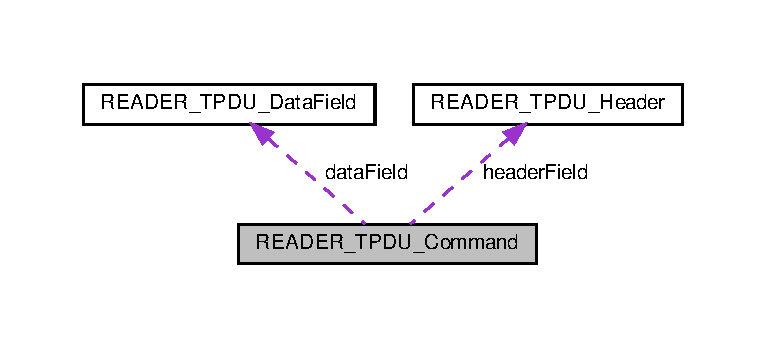
\includegraphics[width=350pt]{struct_r_e_a_d_e_r___t_p_d_u___command__coll__graph}
\end{center}
\end{figure}
\subsection*{Data Fields}
\begin{DoxyCompactItemize}
\item 
\hyperlink{struct_r_e_a_d_e_r___t_p_d_u___header}{R\+E\+A\+D\+E\+R\+\_\+\+T\+P\+D\+U\+\_\+\+Header} \hyperlink{struct_r_e_a_d_e_r___t_p_d_u___command_a03160376b918660c9a47dfc9eeb440f7}{header\+Field}
\item 
\hyperlink{struct_r_e_a_d_e_r___t_p_d_u___data_field}{R\+E\+A\+D\+E\+R\+\_\+\+T\+P\+D\+U\+\_\+\+Data\+Field} \hyperlink{struct_r_e_a_d_e_r___t_p_d_u___command_acbe7f6ca9b7edb9642288240559a2c2b}{data\+Field}
\end{DoxyCompactItemize}


\subsection{Field Documentation}
\mbox{\Hypertarget{struct_r_e_a_d_e_r___t_p_d_u___command_acbe7f6ca9b7edb9642288240559a2c2b}\label{struct_r_e_a_d_e_r___t_p_d_u___command_acbe7f6ca9b7edb9642288240559a2c2b}} 
\index{R\+E\+A\+D\+E\+R\+\_\+\+T\+P\+D\+U\+\_\+\+Command@{R\+E\+A\+D\+E\+R\+\_\+\+T\+P\+D\+U\+\_\+\+Command}!data\+Field@{data\+Field}}
\index{data\+Field@{data\+Field}!R\+E\+A\+D\+E\+R\+\_\+\+T\+P\+D\+U\+\_\+\+Command@{R\+E\+A\+D\+E\+R\+\_\+\+T\+P\+D\+U\+\_\+\+Command}}
\subsubsection{\texorpdfstring{data\+Field}{dataField}}
{\footnotesize\ttfamily \hyperlink{struct_r_e_a_d_e_r___t_p_d_u___data_field}{R\+E\+A\+D\+E\+R\+\_\+\+T\+P\+D\+U\+\_\+\+Data\+Field} data\+Field}

\mbox{\Hypertarget{struct_r_e_a_d_e_r___t_p_d_u___command_a03160376b918660c9a47dfc9eeb440f7}\label{struct_r_e_a_d_e_r___t_p_d_u___command_a03160376b918660c9a47dfc9eeb440f7}} 
\index{R\+E\+A\+D\+E\+R\+\_\+\+T\+P\+D\+U\+\_\+\+Command@{R\+E\+A\+D\+E\+R\+\_\+\+T\+P\+D\+U\+\_\+\+Command}!header\+Field@{header\+Field}}
\index{header\+Field@{header\+Field}!R\+E\+A\+D\+E\+R\+\_\+\+T\+P\+D\+U\+\_\+\+Command@{R\+E\+A\+D\+E\+R\+\_\+\+T\+P\+D\+U\+\_\+\+Command}}
\subsubsection{\texorpdfstring{header\+Field}{headerField}}
{\footnotesize\ttfamily \hyperlink{struct_r_e_a_d_e_r___t_p_d_u___header}{R\+E\+A\+D\+E\+R\+\_\+\+T\+P\+D\+U\+\_\+\+Header} header\+Field}



The documentation for this struct was generated from the following file\+:\begin{DoxyCompactItemize}
\item 
\hyperlink{reader__tpdu_8h}{reader\+\_\+tpdu.\+h}\end{DoxyCompactItemize}

\hypertarget{struct_r_e_a_d_e_r___t_p_d_u___data_field}{}\section{R\+E\+A\+D\+E\+R\+\_\+\+T\+P\+D\+U\+\_\+\+Data\+Field Struct Reference}
\label{struct_r_e_a_d_e_r___t_p_d_u___data_field}\index{R\+E\+A\+D\+E\+R\+\_\+\+T\+P\+D\+U\+\_\+\+Data\+Field@{R\+E\+A\+D\+E\+R\+\_\+\+T\+P\+D\+U\+\_\+\+Data\+Field}}


{\ttfamily \#include $<$reader\+\_\+tpdu.\+h$>$}

\subsection*{Data Fields}
\begin{DoxyCompactItemize}
\item 
uint8\+\_\+t \hyperlink{struct_r_e_a_d_e_r___t_p_d_u___data_field_ae5dc6ffcd9b7605c7787791e40cc6bb0}{size}
\item 
uint8\+\_\+t \hyperlink{struct_r_e_a_d_e_r___t_p_d_u___data_field_ab535cce6473e21eec0352b98db13a53c}{data} \mbox{[}\hyperlink{reader__tpdu_8h_ac2b5682646f650db380874cab59e3e00}{R\+E\+A\+D\+E\+R\+\_\+\+T\+P\+D\+U\+\_\+\+M\+A\+X\+\_\+\+D\+A\+TA}\mbox{]}
\end{DoxyCompactItemize}


\subsection{Field Documentation}
\mbox{\Hypertarget{struct_r_e_a_d_e_r___t_p_d_u___data_field_ab535cce6473e21eec0352b98db13a53c}\label{struct_r_e_a_d_e_r___t_p_d_u___data_field_ab535cce6473e21eec0352b98db13a53c}} 
\index{R\+E\+A\+D\+E\+R\+\_\+\+T\+P\+D\+U\+\_\+\+Data\+Field@{R\+E\+A\+D\+E\+R\+\_\+\+T\+P\+D\+U\+\_\+\+Data\+Field}!data@{data}}
\index{data@{data}!R\+E\+A\+D\+E\+R\+\_\+\+T\+P\+D\+U\+\_\+\+Data\+Field@{R\+E\+A\+D\+E\+R\+\_\+\+T\+P\+D\+U\+\_\+\+Data\+Field}}
\subsubsection{\texorpdfstring{data}{data}}
{\footnotesize\ttfamily uint8\+\_\+t data\mbox{[}\hyperlink{reader__tpdu_8h_ac2b5682646f650db380874cab59e3e00}{R\+E\+A\+D\+E\+R\+\_\+\+T\+P\+D\+U\+\_\+\+M\+A\+X\+\_\+\+D\+A\+TA}\mbox{]}}

\mbox{\Hypertarget{struct_r_e_a_d_e_r___t_p_d_u___data_field_ae5dc6ffcd9b7605c7787791e40cc6bb0}\label{struct_r_e_a_d_e_r___t_p_d_u___data_field_ae5dc6ffcd9b7605c7787791e40cc6bb0}} 
\index{R\+E\+A\+D\+E\+R\+\_\+\+T\+P\+D\+U\+\_\+\+Data\+Field@{R\+E\+A\+D\+E\+R\+\_\+\+T\+P\+D\+U\+\_\+\+Data\+Field}!size@{size}}
\index{size@{size}!R\+E\+A\+D\+E\+R\+\_\+\+T\+P\+D\+U\+\_\+\+Data\+Field@{R\+E\+A\+D\+E\+R\+\_\+\+T\+P\+D\+U\+\_\+\+Data\+Field}}
\subsubsection{\texorpdfstring{size}{size}}
{\footnotesize\ttfamily uint8\+\_\+t size}



The documentation for this struct was generated from the following file\+:\begin{DoxyCompactItemize}
\item 
\hyperlink{reader__tpdu_8h}{reader\+\_\+tpdu.\+h}\end{DoxyCompactItemize}

\hypertarget{struct_r_e_a_d_e_r___t_p_d_u___header}{}\section{R\+E\+A\+D\+E\+R\+\_\+\+T\+P\+D\+U\+\_\+\+Header Struct Reference}
\label{struct_r_e_a_d_e_r___t_p_d_u___header}\index{R\+E\+A\+D\+E\+R\+\_\+\+T\+P\+D\+U\+\_\+\+Header@{R\+E\+A\+D\+E\+R\+\_\+\+T\+P\+D\+U\+\_\+\+Header}}


{\ttfamily \#include $<$reader\+\_\+tpdu.\+h$>$}

\subsection*{Data Fields}
\begin{DoxyCompactItemize}
\item 
uint8\+\_\+t \hyperlink{struct_r_e_a_d_e_r___t_p_d_u___header_a74238fbf52a2f54d07bfd762a35b0717}{C\+LA}
\item 
uint8\+\_\+t \hyperlink{struct_r_e_a_d_e_r___t_p_d_u___header_aa7a3539ade0d2709c339e1959919c47c}{I\+NS}
\item 
uint8\+\_\+t \hyperlink{struct_r_e_a_d_e_r___t_p_d_u___header_a89e93cdfda0a253e4d7ba7948fc4d577}{P1}
\item 
uint8\+\_\+t \hyperlink{struct_r_e_a_d_e_r___t_p_d_u___header_ae927cd0ad523607889b8481386345fea}{P2}
\item 
uint8\+\_\+t \hyperlink{struct_r_e_a_d_e_r___t_p_d_u___header_a782553b6420e66428e37a8b5cf409dc6}{P3}
\end{DoxyCompactItemize}


\subsection{Field Documentation}
\mbox{\Hypertarget{struct_r_e_a_d_e_r___t_p_d_u___header_a74238fbf52a2f54d07bfd762a35b0717}\label{struct_r_e_a_d_e_r___t_p_d_u___header_a74238fbf52a2f54d07bfd762a35b0717}} 
\index{R\+E\+A\+D\+E\+R\+\_\+\+T\+P\+D\+U\+\_\+\+Header@{R\+E\+A\+D\+E\+R\+\_\+\+T\+P\+D\+U\+\_\+\+Header}!C\+LA@{C\+LA}}
\index{C\+LA@{C\+LA}!R\+E\+A\+D\+E\+R\+\_\+\+T\+P\+D\+U\+\_\+\+Header@{R\+E\+A\+D\+E\+R\+\_\+\+T\+P\+D\+U\+\_\+\+Header}}
\subsubsection{\texorpdfstring{C\+LA}{CLA}}
{\footnotesize\ttfamily uint8\+\_\+t C\+LA}

\mbox{\Hypertarget{struct_r_e_a_d_e_r___t_p_d_u___header_aa7a3539ade0d2709c339e1959919c47c}\label{struct_r_e_a_d_e_r___t_p_d_u___header_aa7a3539ade0d2709c339e1959919c47c}} 
\index{R\+E\+A\+D\+E\+R\+\_\+\+T\+P\+D\+U\+\_\+\+Header@{R\+E\+A\+D\+E\+R\+\_\+\+T\+P\+D\+U\+\_\+\+Header}!I\+NS@{I\+NS}}
\index{I\+NS@{I\+NS}!R\+E\+A\+D\+E\+R\+\_\+\+T\+P\+D\+U\+\_\+\+Header@{R\+E\+A\+D\+E\+R\+\_\+\+T\+P\+D\+U\+\_\+\+Header}}
\subsubsection{\texorpdfstring{I\+NS}{INS}}
{\footnotesize\ttfamily uint8\+\_\+t I\+NS}

\mbox{\Hypertarget{struct_r_e_a_d_e_r___t_p_d_u___header_a89e93cdfda0a253e4d7ba7948fc4d577}\label{struct_r_e_a_d_e_r___t_p_d_u___header_a89e93cdfda0a253e4d7ba7948fc4d577}} 
\index{R\+E\+A\+D\+E\+R\+\_\+\+T\+P\+D\+U\+\_\+\+Header@{R\+E\+A\+D\+E\+R\+\_\+\+T\+P\+D\+U\+\_\+\+Header}!P1@{P1}}
\index{P1@{P1}!R\+E\+A\+D\+E\+R\+\_\+\+T\+P\+D\+U\+\_\+\+Header@{R\+E\+A\+D\+E\+R\+\_\+\+T\+P\+D\+U\+\_\+\+Header}}
\subsubsection{\texorpdfstring{P1}{P1}}
{\footnotesize\ttfamily uint8\+\_\+t P1}

\mbox{\Hypertarget{struct_r_e_a_d_e_r___t_p_d_u___header_ae927cd0ad523607889b8481386345fea}\label{struct_r_e_a_d_e_r___t_p_d_u___header_ae927cd0ad523607889b8481386345fea}} 
\index{R\+E\+A\+D\+E\+R\+\_\+\+T\+P\+D\+U\+\_\+\+Header@{R\+E\+A\+D\+E\+R\+\_\+\+T\+P\+D\+U\+\_\+\+Header}!P2@{P2}}
\index{P2@{P2}!R\+E\+A\+D\+E\+R\+\_\+\+T\+P\+D\+U\+\_\+\+Header@{R\+E\+A\+D\+E\+R\+\_\+\+T\+P\+D\+U\+\_\+\+Header}}
\subsubsection{\texorpdfstring{P2}{P2}}
{\footnotesize\ttfamily uint8\+\_\+t P2}

\mbox{\Hypertarget{struct_r_e_a_d_e_r___t_p_d_u___header_a782553b6420e66428e37a8b5cf409dc6}\label{struct_r_e_a_d_e_r___t_p_d_u___header_a782553b6420e66428e37a8b5cf409dc6}} 
\index{R\+E\+A\+D\+E\+R\+\_\+\+T\+P\+D\+U\+\_\+\+Header@{R\+E\+A\+D\+E\+R\+\_\+\+T\+P\+D\+U\+\_\+\+Header}!P3@{P3}}
\index{P3@{P3}!R\+E\+A\+D\+E\+R\+\_\+\+T\+P\+D\+U\+\_\+\+Header@{R\+E\+A\+D\+E\+R\+\_\+\+T\+P\+D\+U\+\_\+\+Header}}
\subsubsection{\texorpdfstring{P3}{P3}}
{\footnotesize\ttfamily uint8\+\_\+t P3}



The documentation for this struct was generated from the following file\+:\begin{DoxyCompactItemize}
\item 
\hyperlink{reader__tpdu_8h}{reader\+\_\+tpdu.\+h}\end{DoxyCompactItemize}

\chapter{File Documentation}
\hypertarget{main_8h}{}\section{main.\+h File Reference}
\label{main_8h}\index{main.\+h@{main.\+h}}
{\ttfamily \#include \char`\"{}stm32f4xx\+\_\+hal.\+h\char`\"{}}\newline
Include dependency graph for main.\+h\+:
\nopagebreak
\begin{figure}[H]
\begin{center}
\leavevmode
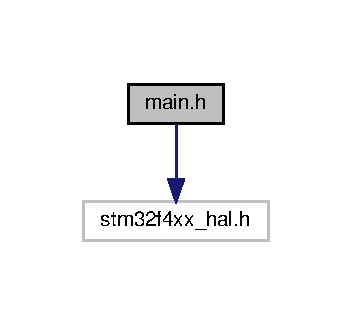
\includegraphics[width=169pt]{main_8h__incl}
\end{center}
\end{figure}
This graph shows which files directly or indirectly include this file\+:
\nopagebreak
\begin{figure}[H]
\begin{center}
\leavevmode
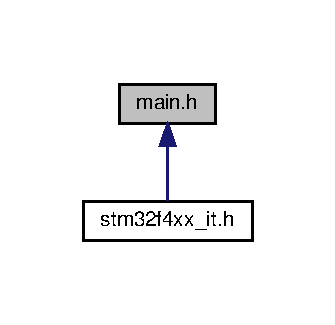
\includegraphics[width=161pt]{main_8h__dep__incl}
\end{center}
\end{figure}
\subsection*{Macros}
\begin{DoxyCompactItemize}
\item 
\#define \hyperlink{main_8h_ac99c1bdc7410c832d5d704fe25dd595f}{P\+I\+N\+\_\+\+L\+E\+D\+\_\+\+V\+E\+R\+TE}~G\+P\+I\+O\+\_\+\+P\+I\+N\+\_\+12       /$\ast$ P\+D12 $\ast$/
\item 
\#define \hyperlink{main_8h_a288f00d0665a36a5e2d806c96ffd5d6a}{P\+I\+N\+\_\+\+L\+E\+D\+\_\+\+R\+O\+U\+GE}~G\+P\+I\+O\+\_\+\+P\+I\+N\+\_\+14       /$\ast$ P\+D14 $\ast$/
\item 
\#define \hyperlink{main_8h_acdc1fc5ae3504a1f0e7ca7d4b54ad850}{P\+I\+N\+\_\+\+B\+O\+U\+T\+O\+N\+\_\+\+B\+L\+EU}~G\+P\+I\+O\+\_\+\+P\+I\+N\+\_\+0      /$\ast$ P\+A0  $\ast$/
\end{DoxyCompactItemize}
\subsection*{Functions}
\begin{DoxyCompactItemize}
\item 
void \hyperlink{main_8h_a0110b02bbe74bf29cc8c83fe96c41b01}{init\+Uart} (void)
\end{DoxyCompactItemize}


\subsection{Macro Definition Documentation}
\mbox{\Hypertarget{main_8h_acdc1fc5ae3504a1f0e7ca7d4b54ad850}\label{main_8h_acdc1fc5ae3504a1f0e7ca7d4b54ad850}} 
\index{main.\+h@{main.\+h}!P\+I\+N\+\_\+\+B\+O\+U\+T\+O\+N\+\_\+\+B\+L\+EU@{P\+I\+N\+\_\+\+B\+O\+U\+T\+O\+N\+\_\+\+B\+L\+EU}}
\index{P\+I\+N\+\_\+\+B\+O\+U\+T\+O\+N\+\_\+\+B\+L\+EU@{P\+I\+N\+\_\+\+B\+O\+U\+T\+O\+N\+\_\+\+B\+L\+EU}!main.\+h@{main.\+h}}
\subsubsection{\texorpdfstring{P\+I\+N\+\_\+\+B\+O\+U\+T\+O\+N\+\_\+\+B\+L\+EU}{PIN\_BOUTON\_BLEU}}
{\footnotesize\ttfamily \#define P\+I\+N\+\_\+\+B\+O\+U\+T\+O\+N\+\_\+\+B\+L\+EU~G\+P\+I\+O\+\_\+\+P\+I\+N\+\_\+0      /$\ast$ P\+A0  $\ast$/}

\mbox{\Hypertarget{main_8h_a288f00d0665a36a5e2d806c96ffd5d6a}\label{main_8h_a288f00d0665a36a5e2d806c96ffd5d6a}} 
\index{main.\+h@{main.\+h}!P\+I\+N\+\_\+\+L\+E\+D\+\_\+\+R\+O\+U\+GE@{P\+I\+N\+\_\+\+L\+E\+D\+\_\+\+R\+O\+U\+GE}}
\index{P\+I\+N\+\_\+\+L\+E\+D\+\_\+\+R\+O\+U\+GE@{P\+I\+N\+\_\+\+L\+E\+D\+\_\+\+R\+O\+U\+GE}!main.\+h@{main.\+h}}
\subsubsection{\texorpdfstring{P\+I\+N\+\_\+\+L\+E\+D\+\_\+\+R\+O\+U\+GE}{PIN\_LED\_ROUGE}}
{\footnotesize\ttfamily \#define P\+I\+N\+\_\+\+L\+E\+D\+\_\+\+R\+O\+U\+GE~G\+P\+I\+O\+\_\+\+P\+I\+N\+\_\+14       /$\ast$ P\+D14 $\ast$/}

\mbox{\Hypertarget{main_8h_ac99c1bdc7410c832d5d704fe25dd595f}\label{main_8h_ac99c1bdc7410c832d5d704fe25dd595f}} 
\index{main.\+h@{main.\+h}!P\+I\+N\+\_\+\+L\+E\+D\+\_\+\+V\+E\+R\+TE@{P\+I\+N\+\_\+\+L\+E\+D\+\_\+\+V\+E\+R\+TE}}
\index{P\+I\+N\+\_\+\+L\+E\+D\+\_\+\+V\+E\+R\+TE@{P\+I\+N\+\_\+\+L\+E\+D\+\_\+\+V\+E\+R\+TE}!main.\+h@{main.\+h}}
\subsubsection{\texorpdfstring{P\+I\+N\+\_\+\+L\+E\+D\+\_\+\+V\+E\+R\+TE}{PIN\_LED\_VERTE}}
{\footnotesize\ttfamily \#define P\+I\+N\+\_\+\+L\+E\+D\+\_\+\+V\+E\+R\+TE~G\+P\+I\+O\+\_\+\+P\+I\+N\+\_\+12       /$\ast$ P\+D12 $\ast$/}



\subsection{Function Documentation}
\mbox{\Hypertarget{main_8h_a0110b02bbe74bf29cc8c83fe96c41b01}\label{main_8h_a0110b02bbe74bf29cc8c83fe96c41b01}} 
\index{main.\+h@{main.\+h}!init\+Uart@{init\+Uart}}
\index{init\+Uart@{init\+Uart}!main.\+h@{main.\+h}}
\subsubsection{\texorpdfstring{init\+Uart()}{initUart()}}
{\footnotesize\ttfamily void init\+Uart (\begin{DoxyParamCaption}\item[{void}]{ }\end{DoxyParamCaption})}


\hypertarget{reader_8h}{}\section{reader.\+h File Reference}
\label{reader_8h}\index{reader.\+h@{reader.\+h}}
This graph shows which files directly or indirectly include this file\+:
\nopagebreak
\begin{figure}[H]
\begin{center}
\leavevmode
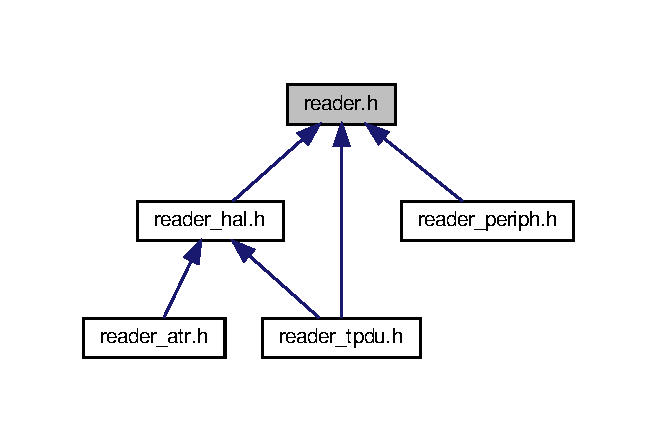
\includegraphics[width=316pt]{reader_8h__dep__incl}
\end{center}
\end{figure}
\subsection*{Macros}
\begin{DoxyCompactItemize}
\item 
\#define \hyperlink{reader_8h_a8027108540a0af74cab295163f43449c}{R\+E\+A\+D\+E\+R\+\_\+\+D\+E\+F\+A\+U\+L\+T\+\_\+\+FI}~(uint32\+\_\+t)(372)
\item 
\#define \hyperlink{reader_8h_abc358ab007ef5f398de3f3dbac2bf581}{R\+E\+A\+D\+E\+R\+\_\+\+D\+E\+F\+A\+U\+L\+T\+\_\+\+DI}~(uint32\+\_\+t)(1)
\item 
\#define \hyperlink{reader_8h_ad5d7b041eac8e3994dc72632e7a600e4}{R\+E\+A\+D\+E\+R\+\_\+\+D\+E\+F\+A\+U\+L\+T\+\_\+\+F\+R\+EQ}~(uint32\+\_\+t)(4200000)
\item 
\#define \hyperlink{reader_8h_ae5b3700acf22e0a446852ee6896f79c7}{R\+E\+A\+D\+E\+R\+\_\+\+D\+E\+F\+A\+U\+L\+T\+\_\+\+GT}~(uint32\+\_\+t)(12)
\item 
\#define \hyperlink{reader_8h_a9b0a3cb19125595530e345b9388ff951}{R\+E\+A\+D\+E\+R\+\_\+\+D\+E\+F\+A\+U\+L\+T\+\_\+\+WI}~(uint32\+\_\+t)(10)
\item 
\#define \hyperlink{reader_8h_af92d2ad954c38570b7fd17ba3d57ee49}{R\+E\+A\+D\+E\+R\+\_\+\+D\+E\+F\+A\+U\+L\+T\+\_\+\+W\+T\+\_\+\+M\+I\+LI}~(uint32\+\_\+t)((1000 $\ast$ \hyperlink{reader_8h_a9b0a3cb19125595530e345b9388ff951}{R\+E\+A\+D\+E\+R\+\_\+\+D\+E\+F\+A\+U\+L\+T\+\_\+\+WI} $\ast$ 960 $\ast$ \hyperlink{reader_8h_a8027108540a0af74cab295163f43449c}{R\+E\+A\+D\+E\+R\+\_\+\+D\+E\+F\+A\+U\+L\+T\+\_\+\+FI}) / \hyperlink{reader_8h_ad5d7b041eac8e3994dc72632e7a600e4}{R\+E\+A\+D\+E\+R\+\_\+\+D\+E\+F\+A\+U\+L\+T\+\_\+\+F\+R\+EQ})      /$\ast$ Voir I\+S\+O7816-\/3 section 10.\+2 $\ast$/
\end{DoxyCompactItemize}
\subsection*{Typedefs}
\begin{DoxyCompactItemize}
\item 
typedef enum \hyperlink{reader_8h_a2ce152a8d1e28c2847301451aa5bbc20}{R\+E\+A\+D\+E\+R\+\_\+\+Status} \hyperlink{reader_8h_af8d3117e6298a67a6a78ba78230d986a}{R\+E\+A\+D\+E\+R\+\_\+\+Status}
\end{DoxyCompactItemize}
\subsection*{Enumerations}
\begin{DoxyCompactItemize}
\item 
enum \hyperlink{reader_8h_a2ce152a8d1e28c2847301451aa5bbc20}{R\+E\+A\+D\+E\+R\+\_\+\+Status} \{ \newline
\hyperlink{reader_8h_a2ce152a8d1e28c2847301451aa5bbc20a4d61387fc27bf9e76c72a78cd165dfff}{R\+E\+A\+D\+E\+R\+\_\+\+OK} = (0x00000001), 
\hyperlink{reader_8h_a2ce152a8d1e28c2847301451aa5bbc20a7c00847c7fde18cb39e1123fa38a6d2b}{R\+E\+A\+D\+E\+R\+\_\+\+NO} = (0x00000000), 
\hyperlink{reader_8h_a2ce152a8d1e28c2847301451aa5bbc20a76f7e652d4489041a23c31b16b02eeb2}{R\+E\+A\+D\+E\+R\+\_\+\+E\+RR} = (0x00000002), 
\hyperlink{reader_8h_a2ce152a8d1e28c2847301451aa5bbc20a4386a7a9d793845b6dce1d2b083b0ab4}{R\+E\+A\+D\+E\+R\+\_\+\+T\+I\+M\+E\+O\+UT} = (0x00000003), 
\newline
\hyperlink{reader_8h_a2ce152a8d1e28c2847301451aa5bbc20a3ceac848e155931d7373b85d8c54eaee}{R\+E\+A\+D\+E\+R\+\_\+\+B\+U\+SY} = (0x00000004)
 \}
\end{DoxyCompactItemize}


\subsection{Macro Definition Documentation}
\mbox{\Hypertarget{reader_8h_abc358ab007ef5f398de3f3dbac2bf581}\label{reader_8h_abc358ab007ef5f398de3f3dbac2bf581}} 
\index{reader.\+h@{reader.\+h}!R\+E\+A\+D\+E\+R\+\_\+\+D\+E\+F\+A\+U\+L\+T\+\_\+\+DI@{R\+E\+A\+D\+E\+R\+\_\+\+D\+E\+F\+A\+U\+L\+T\+\_\+\+DI}}
\index{R\+E\+A\+D\+E\+R\+\_\+\+D\+E\+F\+A\+U\+L\+T\+\_\+\+DI@{R\+E\+A\+D\+E\+R\+\_\+\+D\+E\+F\+A\+U\+L\+T\+\_\+\+DI}!reader.\+h@{reader.\+h}}
\subsubsection{\texorpdfstring{R\+E\+A\+D\+E\+R\+\_\+\+D\+E\+F\+A\+U\+L\+T\+\_\+\+DI}{READER\_DEFAULT\_DI}}
{\footnotesize\ttfamily \#define R\+E\+A\+D\+E\+R\+\_\+\+D\+E\+F\+A\+U\+L\+T\+\_\+\+DI~(uint32\+\_\+t)(1)}

\mbox{\Hypertarget{reader_8h_a8027108540a0af74cab295163f43449c}\label{reader_8h_a8027108540a0af74cab295163f43449c}} 
\index{reader.\+h@{reader.\+h}!R\+E\+A\+D\+E\+R\+\_\+\+D\+E\+F\+A\+U\+L\+T\+\_\+\+FI@{R\+E\+A\+D\+E\+R\+\_\+\+D\+E\+F\+A\+U\+L\+T\+\_\+\+FI}}
\index{R\+E\+A\+D\+E\+R\+\_\+\+D\+E\+F\+A\+U\+L\+T\+\_\+\+FI@{R\+E\+A\+D\+E\+R\+\_\+\+D\+E\+F\+A\+U\+L\+T\+\_\+\+FI}!reader.\+h@{reader.\+h}}
\subsubsection{\texorpdfstring{R\+E\+A\+D\+E\+R\+\_\+\+D\+E\+F\+A\+U\+L\+T\+\_\+\+FI}{READER\_DEFAULT\_FI}}
{\footnotesize\ttfamily \#define R\+E\+A\+D\+E\+R\+\_\+\+D\+E\+F\+A\+U\+L\+T\+\_\+\+FI~(uint32\+\_\+t)(372)}

\mbox{\Hypertarget{reader_8h_ad5d7b041eac8e3994dc72632e7a600e4}\label{reader_8h_ad5d7b041eac8e3994dc72632e7a600e4}} 
\index{reader.\+h@{reader.\+h}!R\+E\+A\+D\+E\+R\+\_\+\+D\+E\+F\+A\+U\+L\+T\+\_\+\+F\+R\+EQ@{R\+E\+A\+D\+E\+R\+\_\+\+D\+E\+F\+A\+U\+L\+T\+\_\+\+F\+R\+EQ}}
\index{R\+E\+A\+D\+E\+R\+\_\+\+D\+E\+F\+A\+U\+L\+T\+\_\+\+F\+R\+EQ@{R\+E\+A\+D\+E\+R\+\_\+\+D\+E\+F\+A\+U\+L\+T\+\_\+\+F\+R\+EQ}!reader.\+h@{reader.\+h}}
\subsubsection{\texorpdfstring{R\+E\+A\+D\+E\+R\+\_\+\+D\+E\+F\+A\+U\+L\+T\+\_\+\+F\+R\+EQ}{READER\_DEFAULT\_FREQ}}
{\footnotesize\ttfamily \#define R\+E\+A\+D\+E\+R\+\_\+\+D\+E\+F\+A\+U\+L\+T\+\_\+\+F\+R\+EQ~(uint32\+\_\+t)(4200000)}

\mbox{\Hypertarget{reader_8h_ae5b3700acf22e0a446852ee6896f79c7}\label{reader_8h_ae5b3700acf22e0a446852ee6896f79c7}} 
\index{reader.\+h@{reader.\+h}!R\+E\+A\+D\+E\+R\+\_\+\+D\+E\+F\+A\+U\+L\+T\+\_\+\+GT@{R\+E\+A\+D\+E\+R\+\_\+\+D\+E\+F\+A\+U\+L\+T\+\_\+\+GT}}
\index{R\+E\+A\+D\+E\+R\+\_\+\+D\+E\+F\+A\+U\+L\+T\+\_\+\+GT@{R\+E\+A\+D\+E\+R\+\_\+\+D\+E\+F\+A\+U\+L\+T\+\_\+\+GT}!reader.\+h@{reader.\+h}}
\subsubsection{\texorpdfstring{R\+E\+A\+D\+E\+R\+\_\+\+D\+E\+F\+A\+U\+L\+T\+\_\+\+GT}{READER\_DEFAULT\_GT}}
{\footnotesize\ttfamily \#define R\+E\+A\+D\+E\+R\+\_\+\+D\+E\+F\+A\+U\+L\+T\+\_\+\+GT~(uint32\+\_\+t)(12)}

\mbox{\Hypertarget{reader_8h_a9b0a3cb19125595530e345b9388ff951}\label{reader_8h_a9b0a3cb19125595530e345b9388ff951}} 
\index{reader.\+h@{reader.\+h}!R\+E\+A\+D\+E\+R\+\_\+\+D\+E\+F\+A\+U\+L\+T\+\_\+\+WI@{R\+E\+A\+D\+E\+R\+\_\+\+D\+E\+F\+A\+U\+L\+T\+\_\+\+WI}}
\index{R\+E\+A\+D\+E\+R\+\_\+\+D\+E\+F\+A\+U\+L\+T\+\_\+\+WI@{R\+E\+A\+D\+E\+R\+\_\+\+D\+E\+F\+A\+U\+L\+T\+\_\+\+WI}!reader.\+h@{reader.\+h}}
\subsubsection{\texorpdfstring{R\+E\+A\+D\+E\+R\+\_\+\+D\+E\+F\+A\+U\+L\+T\+\_\+\+WI}{READER\_DEFAULT\_WI}}
{\footnotesize\ttfamily \#define R\+E\+A\+D\+E\+R\+\_\+\+D\+E\+F\+A\+U\+L\+T\+\_\+\+WI~(uint32\+\_\+t)(10)}

\mbox{\Hypertarget{reader_8h_af92d2ad954c38570b7fd17ba3d57ee49}\label{reader_8h_af92d2ad954c38570b7fd17ba3d57ee49}} 
\index{reader.\+h@{reader.\+h}!R\+E\+A\+D\+E\+R\+\_\+\+D\+E\+F\+A\+U\+L\+T\+\_\+\+W\+T\+\_\+\+M\+I\+LI@{R\+E\+A\+D\+E\+R\+\_\+\+D\+E\+F\+A\+U\+L\+T\+\_\+\+W\+T\+\_\+\+M\+I\+LI}}
\index{R\+E\+A\+D\+E\+R\+\_\+\+D\+E\+F\+A\+U\+L\+T\+\_\+\+W\+T\+\_\+\+M\+I\+LI@{R\+E\+A\+D\+E\+R\+\_\+\+D\+E\+F\+A\+U\+L\+T\+\_\+\+W\+T\+\_\+\+M\+I\+LI}!reader.\+h@{reader.\+h}}
\subsubsection{\texorpdfstring{R\+E\+A\+D\+E\+R\+\_\+\+D\+E\+F\+A\+U\+L\+T\+\_\+\+W\+T\+\_\+\+M\+I\+LI}{READER\_DEFAULT\_WT\_MILI}}
{\footnotesize\ttfamily \#define R\+E\+A\+D\+E\+R\+\_\+\+D\+E\+F\+A\+U\+L\+T\+\_\+\+W\+T\+\_\+\+M\+I\+LI~(uint32\+\_\+t)((1000 $\ast$ \hyperlink{reader_8h_a9b0a3cb19125595530e345b9388ff951}{R\+E\+A\+D\+E\+R\+\_\+\+D\+E\+F\+A\+U\+L\+T\+\_\+\+WI} $\ast$ 960 $\ast$ \hyperlink{reader_8h_a8027108540a0af74cab295163f43449c}{R\+E\+A\+D\+E\+R\+\_\+\+D\+E\+F\+A\+U\+L\+T\+\_\+\+FI}) / \hyperlink{reader_8h_ad5d7b041eac8e3994dc72632e7a600e4}{R\+E\+A\+D\+E\+R\+\_\+\+D\+E\+F\+A\+U\+L\+T\+\_\+\+F\+R\+EQ})      /$\ast$ Voir I\+S\+O7816-\/3 section 10.\+2 $\ast$/}



\subsection{Typedef Documentation}
\mbox{\Hypertarget{reader_8h_af8d3117e6298a67a6a78ba78230d986a}\label{reader_8h_af8d3117e6298a67a6a78ba78230d986a}} 
\index{reader.\+h@{reader.\+h}!R\+E\+A\+D\+E\+R\+\_\+\+Status@{R\+E\+A\+D\+E\+R\+\_\+\+Status}}
\index{R\+E\+A\+D\+E\+R\+\_\+\+Status@{R\+E\+A\+D\+E\+R\+\_\+\+Status}!reader.\+h@{reader.\+h}}
\subsubsection{\texorpdfstring{R\+E\+A\+D\+E\+R\+\_\+\+Status}{READER\_Status}}
{\footnotesize\ttfamily typedef enum \hyperlink{reader_8h_a2ce152a8d1e28c2847301451aa5bbc20}{R\+E\+A\+D\+E\+R\+\_\+\+Status} \hyperlink{reader_8h_a2ce152a8d1e28c2847301451aa5bbc20}{R\+E\+A\+D\+E\+R\+\_\+\+Status}}



\subsection{Enumeration Type Documentation}
\mbox{\Hypertarget{reader_8h_a2ce152a8d1e28c2847301451aa5bbc20}\label{reader_8h_a2ce152a8d1e28c2847301451aa5bbc20}} 
\index{reader.\+h@{reader.\+h}!R\+E\+A\+D\+E\+R\+\_\+\+Status@{R\+E\+A\+D\+E\+R\+\_\+\+Status}}
\index{R\+E\+A\+D\+E\+R\+\_\+\+Status@{R\+E\+A\+D\+E\+R\+\_\+\+Status}!reader.\+h@{reader.\+h}}
\subsubsection{\texorpdfstring{R\+E\+A\+D\+E\+R\+\_\+\+Status}{READER\_Status}}
{\footnotesize\ttfamily enum \hyperlink{reader_8h_a2ce152a8d1e28c2847301451aa5bbc20}{R\+E\+A\+D\+E\+R\+\_\+\+Status}}

\begin{DoxyEnumFields}{Enumerator}
\raisebox{\heightof{T}}[0pt][0pt]{\index{R\+E\+A\+D\+E\+R\+\_\+\+OK@{R\+E\+A\+D\+E\+R\+\_\+\+OK}!reader.\+h@{reader.\+h}}\index{reader.\+h@{reader.\+h}!R\+E\+A\+D\+E\+R\+\_\+\+OK@{R\+E\+A\+D\+E\+R\+\_\+\+OK}}}\mbox{\Hypertarget{reader_8h_a2ce152a8d1e28c2847301451aa5bbc20a4d61387fc27bf9e76c72a78cd165dfff}\label{reader_8h_a2ce152a8d1e28c2847301451aa5bbc20a4d61387fc27bf9e76c72a78cd165dfff}} 
R\+E\+A\+D\+E\+R\+\_\+\+OK&\\
\hline

\raisebox{\heightof{T}}[0pt][0pt]{\index{R\+E\+A\+D\+E\+R\+\_\+\+NO@{R\+E\+A\+D\+E\+R\+\_\+\+NO}!reader.\+h@{reader.\+h}}\index{reader.\+h@{reader.\+h}!R\+E\+A\+D\+E\+R\+\_\+\+NO@{R\+E\+A\+D\+E\+R\+\_\+\+NO}}}\mbox{\Hypertarget{reader_8h_a2ce152a8d1e28c2847301451aa5bbc20a7c00847c7fde18cb39e1123fa38a6d2b}\label{reader_8h_a2ce152a8d1e28c2847301451aa5bbc20a7c00847c7fde18cb39e1123fa38a6d2b}} 
R\+E\+A\+D\+E\+R\+\_\+\+NO&\\
\hline

\raisebox{\heightof{T}}[0pt][0pt]{\index{R\+E\+A\+D\+E\+R\+\_\+\+E\+RR@{R\+E\+A\+D\+E\+R\+\_\+\+E\+RR}!reader.\+h@{reader.\+h}}\index{reader.\+h@{reader.\+h}!R\+E\+A\+D\+E\+R\+\_\+\+E\+RR@{R\+E\+A\+D\+E\+R\+\_\+\+E\+RR}}}\mbox{\Hypertarget{reader_8h_a2ce152a8d1e28c2847301451aa5bbc20a76f7e652d4489041a23c31b16b02eeb2}\label{reader_8h_a2ce152a8d1e28c2847301451aa5bbc20a76f7e652d4489041a23c31b16b02eeb2}} 
R\+E\+A\+D\+E\+R\+\_\+\+E\+RR&\\
\hline

\raisebox{\heightof{T}}[0pt][0pt]{\index{R\+E\+A\+D\+E\+R\+\_\+\+T\+I\+M\+E\+O\+UT@{R\+E\+A\+D\+E\+R\+\_\+\+T\+I\+M\+E\+O\+UT}!reader.\+h@{reader.\+h}}\index{reader.\+h@{reader.\+h}!R\+E\+A\+D\+E\+R\+\_\+\+T\+I\+M\+E\+O\+UT@{R\+E\+A\+D\+E\+R\+\_\+\+T\+I\+M\+E\+O\+UT}}}\mbox{\Hypertarget{reader_8h_a2ce152a8d1e28c2847301451aa5bbc20a4386a7a9d793845b6dce1d2b083b0ab4}\label{reader_8h_a2ce152a8d1e28c2847301451aa5bbc20a4386a7a9d793845b6dce1d2b083b0ab4}} 
R\+E\+A\+D\+E\+R\+\_\+\+T\+I\+M\+E\+O\+UT&\\
\hline

\raisebox{\heightof{T}}[0pt][0pt]{\index{R\+E\+A\+D\+E\+R\+\_\+\+B\+U\+SY@{R\+E\+A\+D\+E\+R\+\_\+\+B\+U\+SY}!reader.\+h@{reader.\+h}}\index{reader.\+h@{reader.\+h}!R\+E\+A\+D\+E\+R\+\_\+\+B\+U\+SY@{R\+E\+A\+D\+E\+R\+\_\+\+B\+U\+SY}}}\mbox{\Hypertarget{reader_8h_a2ce152a8d1e28c2847301451aa5bbc20a3ceac848e155931d7373b85d8c54eaee}\label{reader_8h_a2ce152a8d1e28c2847301451aa5bbc20a3ceac848e155931d7373b85d8c54eaee}} 
R\+E\+A\+D\+E\+R\+\_\+\+B\+U\+SY&\\
\hline

\end{DoxyEnumFields}

\hypertarget{reader__apdu_8h}{}\section{reader\+\_\+apdu.\+h File Reference}
\label{reader__apdu_8h}\index{reader\+\_\+apdu.\+h@{reader\+\_\+apdu.\+h}}

\hypertarget{reader__atr_8h}{}\section{reader\+\_\+atr.\+h File Reference}
\label{reader__atr_8h}\index{reader\+\_\+atr.\+h@{reader\+\_\+atr.\+h}}
{\ttfamily \#include $<$stdint.\+h$>$}\newline
{\ttfamily \#include \char`\"{}reader\+\_\+hal.\+h\char`\"{}}\newline
Include dependency graph for reader\+\_\+atr.\+h\+:
\nopagebreak
\begin{figure}[H]
\begin{center}
\leavevmode
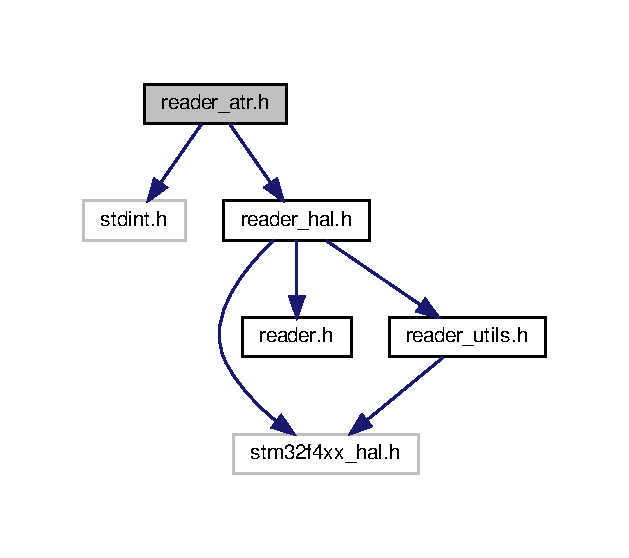
\includegraphics[width=302pt]{reader__atr_8h__incl}
\end{center}
\end{figure}
\subsection*{Data Structures}
\begin{DoxyCompactItemize}
\item 
struct \hyperlink{struct_r_e_a_d_e_r___a_t_r___protocol_specific_bytes}{R\+E\+A\+D\+E\+R\+\_\+\+A\+T\+R\+\_\+\+Protocol\+Specific\+Bytes}
\item 
struct \hyperlink{struct_r_e_a_d_e_r___a_t_r___atr}{R\+E\+A\+D\+E\+R\+\_\+\+A\+T\+R\+\_\+\+Atr}
\end{DoxyCompactItemize}
\subsection*{Macros}
\begin{DoxyCompactItemize}
\item 
\#define \hyperlink{reader__atr_8h_a109a98f6497fb49ae8a3d26693628fa7}{R\+E\+A\+D\+E\+R\+\_\+\+A\+T\+R\+\_\+\+M\+A\+X\+\_\+\+H\+I\+S\+T\+\_\+\+B\+Y\+T\+ES}~15
\item 
\#define \hyperlink{reader__atr_8h_ab72f8cd7d1234d9173796c516f94671f}{R\+E\+A\+D\+E\+R\+\_\+\+A\+T\+R\+\_\+\+M\+A\+X\+\_\+\+S\+P\+E\+C\+I\+F\+I\+C\+\_\+\+B\+Y\+T\+ES}~8
\end{DoxyCompactItemize}
\subsection*{Typedefs}
\begin{DoxyCompactItemize}
\item 
typedef enum \hyperlink{reader__atr_8h_a88b93dcccf6f332cf9a8a08100706e7f}{R\+E\+A\+D\+E\+R\+\_\+\+A\+T\+R\+\_\+\+Clock\+Stop\+Indicator} \hyperlink{reader__atr_8h_aaaaf684be8828c6c5a2120662d658449}{R\+E\+A\+D\+E\+R\+\_\+\+A\+T\+R\+\_\+\+Clock\+Stop\+Indicator}
\item 
typedef enum \hyperlink{reader__atr_8h_a59d38a6964b5cbc4d02b4569618e648b}{R\+E\+A\+D\+E\+R\+\_\+\+A\+T\+R\+\_\+\+Class\+Indicator} \hyperlink{reader__atr_8h_a3e516d68c8f950178e725aa235e29ce8}{R\+E\+A\+D\+E\+R\+\_\+\+A\+T\+R\+\_\+\+Class\+Indicator}
\item 
typedef enum \hyperlink{reader__atr_8h_abefacd0599f2700370b31a1fae95caaf}{R\+E\+A\+D\+E\+R\+\_\+\+A\+T\+R\+\_\+\+Use\+Of\+S\+PU} \hyperlink{reader__atr_8h_af61abefd746e4e1ee0267041e4575e2b}{R\+E\+A\+D\+E\+R\+\_\+\+A\+T\+R\+\_\+\+Use\+Of\+S\+PU}
\item 
typedef enum \hyperlink{reader__atr_8h_a193a4a51751968ed8d31224726c2b967}{R\+E\+A\+D\+E\+R\+\_\+\+A\+T\+R\+\_\+\+Encoding\+Conv} \hyperlink{reader__atr_8h_a30596eb4e363ef10e6e8ec072cf6a183}{R\+E\+A\+D\+E\+R\+\_\+\+A\+T\+R\+\_\+\+Encoding\+Conv}
\item 
typedef struct \hyperlink{struct_r_e_a_d_e_r___a_t_r___protocol_specific_bytes}{R\+E\+A\+D\+E\+R\+\_\+\+A\+T\+R\+\_\+\+Protocol\+Specific\+Bytes} \hyperlink{reader__atr_8h_ae07b2cec0ef16fd5c1fdbe06d10a0b04}{R\+E\+A\+D\+E\+R\+\_\+\+A\+T\+R\+\_\+\+Protocol\+Specific\+Bytes}
\item 
typedef struct \hyperlink{struct_r_e_a_d_e_r___a_t_r___atr}{R\+E\+A\+D\+E\+R\+\_\+\+A\+T\+R\+\_\+\+Atr} \hyperlink{reader__atr_8h_ac48e98c6bdb245db08937df8182d4c2f}{R\+E\+A\+D\+E\+R\+\_\+\+A\+T\+R\+\_\+\+Atr}
\end{DoxyCompactItemize}
\subsection*{Enumerations}
\begin{DoxyCompactItemize}
\item 
enum \hyperlink{reader__atr_8h_a88b93dcccf6f332cf9a8a08100706e7f}{R\+E\+A\+D\+E\+R\+\_\+\+A\+T\+R\+\_\+\+Clock\+Stop\+Indicator} \{ \newline
\hyperlink{reader__atr_8h_a88b93dcccf6f332cf9a8a08100706e7fa9acaed68af52e61f335ac24a881e3049}{R\+E\+A\+D\+E\+R\+\_\+\+A\+T\+R\+\_\+\+C\+L\+O\+C\+K\+S\+T\+O\+P\+\_\+\+N\+O\+T\+S\+U\+P\+P\+O\+R\+T\+ED} = (uint32\+\_\+t)(0x00000000), 
\hyperlink{reader__atr_8h_a88b93dcccf6f332cf9a8a08100706e7fad58f81b58c7a365aeae05b4a9ba2e7f5}{R\+E\+A\+D\+E\+R\+\_\+\+A\+T\+R\+\_\+\+C\+L\+O\+C\+K\+S\+T\+O\+P\+\_\+\+S\+T\+A\+T\+E\+\_\+L} = (uint32\+\_\+t)(0x00000001), 
\hyperlink{reader__atr_8h_a88b93dcccf6f332cf9a8a08100706e7fabe750841f558dcb1b8fc3ccf80900403}{R\+E\+A\+D\+E\+R\+\_\+\+A\+T\+R\+\_\+\+C\+L\+O\+C\+K\+S\+T\+O\+P\+\_\+\+S\+T\+A\+T\+E\+\_\+H} = (uint32\+\_\+t)(0x00000002), 
\hyperlink{reader__atr_8h_a88b93dcccf6f332cf9a8a08100706e7fad5a6c1120c70f709a2addd74003f1a6a}{R\+E\+A\+D\+E\+R\+\_\+\+A\+T\+R\+\_\+\+C\+L\+O\+C\+K\+S\+T\+O\+P\+\_\+\+N\+O\+P\+R\+EF} = (uint32\+\_\+t)(0x00000003), 
\newline
\hyperlink{reader__atr_8h_a88b93dcccf6f332cf9a8a08100706e7fa6171c1d6b6f945f86905f117f4a997f1}{R\+E\+A\+D\+E\+R\+\_\+\+A\+T\+R\+\_\+\+C\+L\+O\+C\+K\+S\+T\+O\+P\+\_\+\+N\+O\+T\+I\+N\+D\+I\+C\+A\+T\+ED} = (uint32\+\_\+t)(0x00000004)
 \}
\item 
enum \hyperlink{reader__atr_8h_a59d38a6964b5cbc4d02b4569618e648b}{R\+E\+A\+D\+E\+R\+\_\+\+A\+T\+R\+\_\+\+Class\+Indicator} \{ \newline
\hyperlink{reader__atr_8h_a59d38a6964b5cbc4d02b4569618e648baba82659689056e99e7f13bdf878404f9}{R\+E\+A\+D\+E\+R\+\_\+\+A\+T\+R\+\_\+\+C\+L\+A\+S\+S\+\_\+\+A\+\_\+\+O\+N\+LY} = (uint32\+\_\+t)(0x00000001), 
\hyperlink{reader__atr_8h_a59d38a6964b5cbc4d02b4569618e648babb1ba133c3639470e0580b562342e551}{R\+E\+A\+D\+E\+R\+\_\+\+A\+T\+R\+\_\+\+C\+L\+A\+S\+S\+\_\+\+B\+\_\+\+O\+N\+LY} = (uint32\+\_\+t)(0x00000002), 
\hyperlink{reader__atr_8h_a59d38a6964b5cbc4d02b4569618e648ba4bdd21523a74ce6288c249779a9ca3b2}{R\+E\+A\+D\+E\+R\+\_\+\+A\+T\+R\+\_\+\+C\+L\+A\+S\+S\+\_\+\+C\+\_\+\+O\+N\+LY} = (uint32\+\_\+t)(0x00000004), 
\hyperlink{reader__atr_8h_a59d38a6964b5cbc4d02b4569618e648ba0a67bc1cb837e49c281bfe10810d8a0e}{R\+E\+A\+D\+E\+R\+\_\+\+A\+T\+R\+\_\+\+C\+L\+A\+S\+S\+\_\+\+A\+B\+\_\+\+O\+N\+LY} = (uint32\+\_\+t)(0x00000003), 
\newline
\hyperlink{reader__atr_8h_a59d38a6964b5cbc4d02b4569618e648ba403f7e7d11f12fb27221e2d1aeee3189}{R\+E\+A\+D\+E\+R\+\_\+\+A\+T\+R\+\_\+\+C\+L\+A\+S\+S\+\_\+\+B\+C\+\_\+\+O\+N\+LY} = (uint32\+\_\+t)(0x00000006), 
\hyperlink{reader__atr_8h_a59d38a6964b5cbc4d02b4569618e648baf4716da3dc1b6ec2f5aa6e76362f75af}{R\+E\+A\+D\+E\+R\+\_\+\+A\+T\+R\+\_\+\+C\+L\+A\+S\+S\+\_\+\+A\+BC} = (uint32\+\_\+t)(0x00000007), 
\hyperlink{reader__atr_8h_a59d38a6964b5cbc4d02b4569618e648ba4ccc4a9eb408f2dccb39347bc2a65dba}{R\+E\+A\+D\+E\+R\+\_\+\+A\+T\+R\+\_\+\+C\+L\+A\+S\+S\+\_\+\+N\+O\+T\+I\+N\+D\+I\+C\+A\+T\+ED} = (uint32\+\_\+t)(0x00000000)
 \}
\item 
enum \hyperlink{reader__atr_8h_abefacd0599f2700370b31a1fae95caaf}{R\+E\+A\+D\+E\+R\+\_\+\+A\+T\+R\+\_\+\+Use\+Of\+S\+PU} \{ \hyperlink{reader__atr_8h_abefacd0599f2700370b31a1fae95caafaed2faed286311faffacbf358e29054ad}{R\+E\+A\+D\+E\+R\+\_\+\+A\+T\+R\+\_\+\+S\+P\+U\+\_\+\+S\+T\+A\+N\+D\+A\+RD} = (uint32\+\_\+t)(0x00000002), 
\hyperlink{reader__atr_8h_abefacd0599f2700370b31a1fae95caafa0df2410220a2ad7f52a5cc91f0620f0a}{R\+E\+A\+D\+E\+R\+\_\+\+A\+T\+R\+\_\+\+S\+P\+U\+\_\+\+P\+R\+O\+P\+R\+I\+E\+T\+A\+RY} = (uint32\+\_\+t)(0x00000001), 
\hyperlink{reader__atr_8h_abefacd0599f2700370b31a1fae95caafad9eb23defb93dc0e9197c7274057067a}{R\+E\+A\+D\+E\+R\+\_\+\+A\+T\+R\+\_\+\+S\+P\+U\+\_\+\+N\+O\+T\+U\+S\+ED} = (uint32\+\_\+t)(0x00000000), 
\hyperlink{reader__atr_8h_abefacd0599f2700370b31a1fae95caafa191659439f1ad706f97e019eb8bbaab6}{R\+E\+A\+D\+E\+R\+\_\+\+A\+T\+R\+\_\+\+S\+P\+U\+\_\+\+N\+O\+T\+I\+N\+D\+I\+C\+A\+T\+ED} = (uint32\+\_\+t)(0x00000003)
 \}
\item 
enum \hyperlink{reader__atr_8h_a193a4a51751968ed8d31224726c2b967}{R\+E\+A\+D\+E\+R\+\_\+\+A\+T\+R\+\_\+\+Encoding\+Conv} \{ \hyperlink{reader__atr_8h_a193a4a51751968ed8d31224726c2b967a453f1ed8f542c88d72c797fc26f8a28e}{R\+E\+A\+D\+E\+R\+\_\+\+A\+T\+R\+\_\+\+E\+N\+C\+O\+D\+I\+N\+G\+\_\+\+D\+I\+R\+E\+CT} = (uint32\+\_\+t)(0x0000003B), 
\hyperlink{reader__atr_8h_a193a4a51751968ed8d31224726c2b967a87d9649b081248424b2163a9456a0269}{R\+E\+A\+D\+E\+R\+\_\+\+A\+T\+R\+\_\+\+E\+N\+C\+O\+D\+I\+N\+G\+\_\+\+R\+E\+V\+E\+R\+SE} = (uint32\+\_\+t)(0x00000003)
 \}
\end{DoxyCompactItemize}
\subsection*{Functions}
\begin{DoxyCompactItemize}
\item 
\hyperlink{reader_8h_a2ce152a8d1e28c2847301451aa5bbc20}{R\+E\+A\+D\+E\+R\+\_\+\+Status} \hyperlink{reader__atr_8h_ad2aeae744315d7dcbce61c418f740a99}{R\+E\+A\+D\+E\+R\+\_\+\+A\+T\+R\+\_\+\+Is\+Interfaces\+Bytes\+To\+Read} (uint8\+\_\+t Y)
\item 
\hyperlink{reader_8h_a2ce152a8d1e28c2847301451aa5bbc20}{R\+E\+A\+D\+E\+R\+\_\+\+Status} \hyperlink{reader__atr_8h_a9765663cf9b759ab8030d09dbffcf1d1}{R\+E\+A\+D\+E\+R\+\_\+\+A\+T\+R\+\_\+\+Is\+T\+A\+To\+Read} (uint8\+\_\+t Y)
\item 
\hyperlink{reader_8h_a2ce152a8d1e28c2847301451aa5bbc20}{R\+E\+A\+D\+E\+R\+\_\+\+Status} \hyperlink{reader__atr_8h_a54d36b36391e7796ceacc2a9d7a578ef}{R\+E\+A\+D\+E\+R\+\_\+\+A\+T\+R\+\_\+\+Is\+T\+B\+To\+Read} (uint8\+\_\+t Y)
\item 
\hyperlink{reader_8h_a2ce152a8d1e28c2847301451aa5bbc20}{R\+E\+A\+D\+E\+R\+\_\+\+Status} \hyperlink{reader__atr_8h_a3f54fc33f9ea1fbb8f50deb6fcd04e23}{R\+E\+A\+D\+E\+R\+\_\+\+A\+T\+R\+\_\+\+Is\+T\+C\+To\+Read} (uint8\+\_\+t Y)
\item 
\hyperlink{reader_8h_a2ce152a8d1e28c2847301451aa5bbc20}{R\+E\+A\+D\+E\+R\+\_\+\+Status} \hyperlink{reader__atr_8h_ae62b8e2b301a1d2eab4eb26d40a16d31}{R\+E\+A\+D\+E\+R\+\_\+\+A\+T\+R\+\_\+\+Is\+T\+D\+To\+Read} (uint8\+\_\+t Y)
\item 
\hyperlink{reader_8h_a2ce152a8d1e28c2847301451aa5bbc20}{R\+E\+A\+D\+E\+R\+\_\+\+Status} \hyperlink{reader__atr_8h_aae96e6fed649fbb45801ea07f52fc6ce}{R\+E\+A\+D\+E\+R\+\_\+\+A\+T\+R\+\_\+\+Process\+TA} (\hyperlink{struct_r_e_a_d_e_r___a_t_r___atr}{R\+E\+A\+D\+E\+R\+\_\+\+A\+T\+R\+\_\+\+Atr} $\ast$atr, uint8\+\_\+t TA, uint32\+\_\+t i, uint8\+\_\+t T)
\item 
\hyperlink{reader_8h_a2ce152a8d1e28c2847301451aa5bbc20}{R\+E\+A\+D\+E\+R\+\_\+\+Status} \hyperlink{reader__atr_8h_a539ee0d503275af9cc8948044ef09c2f}{R\+E\+A\+D\+E\+R\+\_\+\+A\+T\+R\+\_\+\+Process\+TB} (\hyperlink{struct_r_e_a_d_e_r___a_t_r___atr}{R\+E\+A\+D\+E\+R\+\_\+\+A\+T\+R\+\_\+\+Atr} $\ast$atr, uint8\+\_\+t TB, uint32\+\_\+t i, uint8\+\_\+t T)
\item 
\hyperlink{reader_8h_a2ce152a8d1e28c2847301451aa5bbc20}{R\+E\+A\+D\+E\+R\+\_\+\+Status} \hyperlink{reader__atr_8h_a42de1644fe8c65452b363f07433edfc4}{R\+E\+A\+D\+E\+R\+\_\+\+A\+T\+R\+\_\+\+Process\+TC} (\hyperlink{struct_r_e_a_d_e_r___a_t_r___atr}{R\+E\+A\+D\+E\+R\+\_\+\+A\+T\+R\+\_\+\+Atr} $\ast$atr, uint8\+\_\+t TC, uint32\+\_\+t i, uint8\+\_\+t T)
\item 
uint8\+\_\+t \hyperlink{reader__atr_8h_a17753a833e4d0ca4f37f16bbe03c0f12}{R\+E\+A\+D\+E\+R\+\_\+\+A\+T\+R\+\_\+\+GetY} (uint8\+\_\+t TD)
\item 
uint8\+\_\+t \hyperlink{reader__atr_8h_a16d328ef453dee135e416543d0cb6b54}{R\+E\+A\+D\+E\+R\+\_\+\+A\+T\+R\+\_\+\+GetT} (uint8\+\_\+t TD)
\item 
uint8\+\_\+t \hyperlink{reader__atr_8h_ab3102ed833a86dea7d1ae1481bf0b1d0}{R\+E\+A\+D\+E\+R\+\_\+\+A\+T\+R\+\_\+\+GetK} (uint8\+\_\+t T0)
\item 
uint32\+\_\+t \hyperlink{reader__atr_8h_af8d004c580ed2bf83c6da904eb834391}{R\+E\+A\+D\+E\+R\+\_\+\+A\+T\+R\+\_\+\+Get\+Fi} (uint8\+\_\+t T\+A1)
\item 
uint32\+\_\+t \hyperlink{reader__atr_8h_a16f1559422f2ff38f9197c9349556922}{R\+E\+A\+D\+E\+R\+\_\+\+A\+T\+R\+\_\+\+Get\+F\+Max} (uint8\+\_\+t T\+A1)
\item 
uint32\+\_\+t \hyperlink{reader__atr_8h_a2858f5047fc30ff2d58fa0935ae550eb}{R\+E\+A\+D\+E\+R\+\_\+\+A\+T\+R\+\_\+\+Get\+Di} (uint8\+\_\+t T\+A1)
\item 
\hyperlink{reader__atr_8h_a88b93dcccf6f332cf9a8a08100706e7f}{R\+E\+A\+D\+E\+R\+\_\+\+A\+T\+R\+\_\+\+Clock\+Stop\+Indicator} \hyperlink{reader__atr_8h_aa191170f40a33f5a01188d8864ee2777}{R\+E\+A\+D\+E\+R\+\_\+\+A\+T\+R\+\_\+\+Get\+Clock\+Stop\+Indic} (uint8\+\_\+t T\+A15)
\item 
\hyperlink{reader__atr_8h_a59d38a6964b5cbc4d02b4569618e648b}{R\+E\+A\+D\+E\+R\+\_\+\+A\+T\+R\+\_\+\+Class\+Indicator} \hyperlink{reader__atr_8h_a28ece4dfa74235a205a1e7baf42ac901}{R\+E\+A\+D\+E\+R\+\_\+\+A\+T\+R\+\_\+\+Get\+Class\+Indic} (uint8\+\_\+t T\+A15)
\item 
\hyperlink{reader__atr_8h_abefacd0599f2700370b31a1fae95caaf}{R\+E\+A\+D\+E\+R\+\_\+\+A\+T\+R\+\_\+\+Use\+Of\+S\+PU} \hyperlink{reader__atr_8h_ae9c8bc2017b2daaf4bfe8b5ac2b0ccfd}{R\+E\+A\+D\+E\+R\+\_\+\+A\+T\+R\+\_\+\+Get\+Use\+S\+PU} (uint8\+\_\+t T\+B15)
\item 
\hyperlink{reader__atr_8h_a193a4a51751968ed8d31224726c2b967}{R\+E\+A\+D\+E\+R\+\_\+\+A\+T\+R\+\_\+\+Encoding\+Conv} \hyperlink{reader__atr_8h_a3bc9786fa7ab35fd724dd71f74550806}{R\+E\+A\+D\+E\+R\+\_\+\+A\+T\+R\+\_\+\+Get\+Encoding} (uint8\+\_\+t TS)
\item 
\hyperlink{reader_8h_a2ce152a8d1e28c2847301451aa5bbc20}{R\+E\+A\+D\+E\+R\+\_\+\+Status} \hyperlink{reader__atr_8h_a5d9c3440de1e8517d1b79316e648980e}{R\+E\+A\+D\+E\+R\+\_\+\+A\+T\+R\+\_\+\+Receive} (\hyperlink{struct_r_e_a_d_e_r___a_t_r___atr}{R\+E\+A\+D\+E\+R\+\_\+\+A\+T\+R\+\_\+\+Atr} $\ast$atr)
\item 
\hyperlink{reader_8h_a2ce152a8d1e28c2847301451aa5bbc20}{R\+E\+A\+D\+E\+R\+\_\+\+Status} \hyperlink{reader__atr_8h_a6f0b64ea70312d4a36fc0277346a1990}{R\+E\+A\+D\+E\+R\+\_\+\+A\+T\+R\+\_\+\+Init\+Struct} (\hyperlink{struct_r_e_a_d_e_r___a_t_r___atr}{R\+E\+A\+D\+E\+R\+\_\+\+A\+T\+R\+\_\+\+Atr} $\ast$atr)
\item 
void \hyperlink{reader__atr_8h_af47631c8cd518801d8db73054b0662e3}{R\+E\+A\+D\+E\+R\+\_\+\+A\+T\+R\+\_\+\+Err\+Handler} (void)
\item 
\hyperlink{reader_8h_a2ce152a8d1e28c2847301451aa5bbc20}{R\+E\+A\+D\+E\+R\+\_\+\+Status} \hyperlink{reader__atr_8h_a89a97de8ffb281a3ac340b859baf09c3}{R\+E\+A\+D\+E\+R\+\_\+\+A\+T\+R\+\_\+\+Check\+TS} (uint8\+\_\+t TS)
\end{DoxyCompactItemize}


\subsection{Macro Definition Documentation}
\mbox{\Hypertarget{reader__atr_8h_a109a98f6497fb49ae8a3d26693628fa7}\label{reader__atr_8h_a109a98f6497fb49ae8a3d26693628fa7}} 
\index{reader\+\_\+atr.\+h@{reader\+\_\+atr.\+h}!R\+E\+A\+D\+E\+R\+\_\+\+A\+T\+R\+\_\+\+M\+A\+X\+\_\+\+H\+I\+S\+T\+\_\+\+B\+Y\+T\+ES@{R\+E\+A\+D\+E\+R\+\_\+\+A\+T\+R\+\_\+\+M\+A\+X\+\_\+\+H\+I\+S\+T\+\_\+\+B\+Y\+T\+ES}}
\index{R\+E\+A\+D\+E\+R\+\_\+\+A\+T\+R\+\_\+\+M\+A\+X\+\_\+\+H\+I\+S\+T\+\_\+\+B\+Y\+T\+ES@{R\+E\+A\+D\+E\+R\+\_\+\+A\+T\+R\+\_\+\+M\+A\+X\+\_\+\+H\+I\+S\+T\+\_\+\+B\+Y\+T\+ES}!reader\+\_\+atr.\+h@{reader\+\_\+atr.\+h}}
\subsubsection{\texorpdfstring{R\+E\+A\+D\+E\+R\+\_\+\+A\+T\+R\+\_\+\+M\+A\+X\+\_\+\+H\+I\+S\+T\+\_\+\+B\+Y\+T\+ES}{READER\_ATR\_MAX\_HIST\_BYTES}}
{\footnotesize\ttfamily \#define R\+E\+A\+D\+E\+R\+\_\+\+A\+T\+R\+\_\+\+M\+A\+X\+\_\+\+H\+I\+S\+T\+\_\+\+B\+Y\+T\+ES~15}

\mbox{\Hypertarget{reader__atr_8h_ab72f8cd7d1234d9173796c516f94671f}\label{reader__atr_8h_ab72f8cd7d1234d9173796c516f94671f}} 
\index{reader\+\_\+atr.\+h@{reader\+\_\+atr.\+h}!R\+E\+A\+D\+E\+R\+\_\+\+A\+T\+R\+\_\+\+M\+A\+X\+\_\+\+S\+P\+E\+C\+I\+F\+I\+C\+\_\+\+B\+Y\+T\+ES@{R\+E\+A\+D\+E\+R\+\_\+\+A\+T\+R\+\_\+\+M\+A\+X\+\_\+\+S\+P\+E\+C\+I\+F\+I\+C\+\_\+\+B\+Y\+T\+ES}}
\index{R\+E\+A\+D\+E\+R\+\_\+\+A\+T\+R\+\_\+\+M\+A\+X\+\_\+\+S\+P\+E\+C\+I\+F\+I\+C\+\_\+\+B\+Y\+T\+ES@{R\+E\+A\+D\+E\+R\+\_\+\+A\+T\+R\+\_\+\+M\+A\+X\+\_\+\+S\+P\+E\+C\+I\+F\+I\+C\+\_\+\+B\+Y\+T\+ES}!reader\+\_\+atr.\+h@{reader\+\_\+atr.\+h}}
\subsubsection{\texorpdfstring{R\+E\+A\+D\+E\+R\+\_\+\+A\+T\+R\+\_\+\+M\+A\+X\+\_\+\+S\+P\+E\+C\+I\+F\+I\+C\+\_\+\+B\+Y\+T\+ES}{READER\_ATR\_MAX\_SPECIFIC\_BYTES}}
{\footnotesize\ttfamily \#define R\+E\+A\+D\+E\+R\+\_\+\+A\+T\+R\+\_\+\+M\+A\+X\+\_\+\+S\+P\+E\+C\+I\+F\+I\+C\+\_\+\+B\+Y\+T\+ES~8}



\subsection{Typedef Documentation}
\mbox{\Hypertarget{reader__atr_8h_ac48e98c6bdb245db08937df8182d4c2f}\label{reader__atr_8h_ac48e98c6bdb245db08937df8182d4c2f}} 
\index{reader\+\_\+atr.\+h@{reader\+\_\+atr.\+h}!R\+E\+A\+D\+E\+R\+\_\+\+A\+T\+R\+\_\+\+Atr@{R\+E\+A\+D\+E\+R\+\_\+\+A\+T\+R\+\_\+\+Atr}}
\index{R\+E\+A\+D\+E\+R\+\_\+\+A\+T\+R\+\_\+\+Atr@{R\+E\+A\+D\+E\+R\+\_\+\+A\+T\+R\+\_\+\+Atr}!reader\+\_\+atr.\+h@{reader\+\_\+atr.\+h}}
\subsubsection{\texorpdfstring{R\+E\+A\+D\+E\+R\+\_\+\+A\+T\+R\+\_\+\+Atr}{READER\_ATR\_Atr}}
{\footnotesize\ttfamily typedef struct \hyperlink{struct_r_e_a_d_e_r___a_t_r___atr}{R\+E\+A\+D\+E\+R\+\_\+\+A\+T\+R\+\_\+\+Atr} \hyperlink{struct_r_e_a_d_e_r___a_t_r___atr}{R\+E\+A\+D\+E\+R\+\_\+\+A\+T\+R\+\_\+\+Atr}}

\mbox{\Hypertarget{reader__atr_8h_a3e516d68c8f950178e725aa235e29ce8}\label{reader__atr_8h_a3e516d68c8f950178e725aa235e29ce8}} 
\index{reader\+\_\+atr.\+h@{reader\+\_\+atr.\+h}!R\+E\+A\+D\+E\+R\+\_\+\+A\+T\+R\+\_\+\+Class\+Indicator@{R\+E\+A\+D\+E\+R\+\_\+\+A\+T\+R\+\_\+\+Class\+Indicator}}
\index{R\+E\+A\+D\+E\+R\+\_\+\+A\+T\+R\+\_\+\+Class\+Indicator@{R\+E\+A\+D\+E\+R\+\_\+\+A\+T\+R\+\_\+\+Class\+Indicator}!reader\+\_\+atr.\+h@{reader\+\_\+atr.\+h}}
\subsubsection{\texorpdfstring{R\+E\+A\+D\+E\+R\+\_\+\+A\+T\+R\+\_\+\+Class\+Indicator}{READER\_ATR\_ClassIndicator}}
{\footnotesize\ttfamily typedef enum \hyperlink{reader__atr_8h_a59d38a6964b5cbc4d02b4569618e648b}{R\+E\+A\+D\+E\+R\+\_\+\+A\+T\+R\+\_\+\+Class\+Indicator} \hyperlink{reader__atr_8h_a59d38a6964b5cbc4d02b4569618e648b}{R\+E\+A\+D\+E\+R\+\_\+\+A\+T\+R\+\_\+\+Class\+Indicator}}

\mbox{\Hypertarget{reader__atr_8h_aaaaf684be8828c6c5a2120662d658449}\label{reader__atr_8h_aaaaf684be8828c6c5a2120662d658449}} 
\index{reader\+\_\+atr.\+h@{reader\+\_\+atr.\+h}!R\+E\+A\+D\+E\+R\+\_\+\+A\+T\+R\+\_\+\+Clock\+Stop\+Indicator@{R\+E\+A\+D\+E\+R\+\_\+\+A\+T\+R\+\_\+\+Clock\+Stop\+Indicator}}
\index{R\+E\+A\+D\+E\+R\+\_\+\+A\+T\+R\+\_\+\+Clock\+Stop\+Indicator@{R\+E\+A\+D\+E\+R\+\_\+\+A\+T\+R\+\_\+\+Clock\+Stop\+Indicator}!reader\+\_\+atr.\+h@{reader\+\_\+atr.\+h}}
\subsubsection{\texorpdfstring{R\+E\+A\+D\+E\+R\+\_\+\+A\+T\+R\+\_\+\+Clock\+Stop\+Indicator}{READER\_ATR\_ClockStopIndicator}}
{\footnotesize\ttfamily typedef enum \hyperlink{reader__atr_8h_a88b93dcccf6f332cf9a8a08100706e7f}{R\+E\+A\+D\+E\+R\+\_\+\+A\+T\+R\+\_\+\+Clock\+Stop\+Indicator} \hyperlink{reader__atr_8h_a88b93dcccf6f332cf9a8a08100706e7f}{R\+E\+A\+D\+E\+R\+\_\+\+A\+T\+R\+\_\+\+Clock\+Stop\+Indicator}}

\mbox{\Hypertarget{reader__atr_8h_a30596eb4e363ef10e6e8ec072cf6a183}\label{reader__atr_8h_a30596eb4e363ef10e6e8ec072cf6a183}} 
\index{reader\+\_\+atr.\+h@{reader\+\_\+atr.\+h}!R\+E\+A\+D\+E\+R\+\_\+\+A\+T\+R\+\_\+\+Encoding\+Conv@{R\+E\+A\+D\+E\+R\+\_\+\+A\+T\+R\+\_\+\+Encoding\+Conv}}
\index{R\+E\+A\+D\+E\+R\+\_\+\+A\+T\+R\+\_\+\+Encoding\+Conv@{R\+E\+A\+D\+E\+R\+\_\+\+A\+T\+R\+\_\+\+Encoding\+Conv}!reader\+\_\+atr.\+h@{reader\+\_\+atr.\+h}}
\subsubsection{\texorpdfstring{R\+E\+A\+D\+E\+R\+\_\+\+A\+T\+R\+\_\+\+Encoding\+Conv}{READER\_ATR\_EncodingConv}}
{\footnotesize\ttfamily typedef enum \hyperlink{reader__atr_8h_a193a4a51751968ed8d31224726c2b967}{R\+E\+A\+D\+E\+R\+\_\+\+A\+T\+R\+\_\+\+Encoding\+Conv} \hyperlink{reader__atr_8h_a193a4a51751968ed8d31224726c2b967}{R\+E\+A\+D\+E\+R\+\_\+\+A\+T\+R\+\_\+\+Encoding\+Conv}}

\mbox{\Hypertarget{reader__atr_8h_ae07b2cec0ef16fd5c1fdbe06d10a0b04}\label{reader__atr_8h_ae07b2cec0ef16fd5c1fdbe06d10a0b04}} 
\index{reader\+\_\+atr.\+h@{reader\+\_\+atr.\+h}!R\+E\+A\+D\+E\+R\+\_\+\+A\+T\+R\+\_\+\+Protocol\+Specific\+Bytes@{R\+E\+A\+D\+E\+R\+\_\+\+A\+T\+R\+\_\+\+Protocol\+Specific\+Bytes}}
\index{R\+E\+A\+D\+E\+R\+\_\+\+A\+T\+R\+\_\+\+Protocol\+Specific\+Bytes@{R\+E\+A\+D\+E\+R\+\_\+\+A\+T\+R\+\_\+\+Protocol\+Specific\+Bytes}!reader\+\_\+atr.\+h@{reader\+\_\+atr.\+h}}
\subsubsection{\texorpdfstring{R\+E\+A\+D\+E\+R\+\_\+\+A\+T\+R\+\_\+\+Protocol\+Specific\+Bytes}{READER\_ATR\_ProtocolSpecificBytes}}
{\footnotesize\ttfamily typedef struct \hyperlink{struct_r_e_a_d_e_r___a_t_r___protocol_specific_bytes}{R\+E\+A\+D\+E\+R\+\_\+\+A\+T\+R\+\_\+\+Protocol\+Specific\+Bytes} \hyperlink{struct_r_e_a_d_e_r___a_t_r___protocol_specific_bytes}{R\+E\+A\+D\+E\+R\+\_\+\+A\+T\+R\+\_\+\+Protocol\+Specific\+Bytes}}

\mbox{\Hypertarget{reader__atr_8h_af61abefd746e4e1ee0267041e4575e2b}\label{reader__atr_8h_af61abefd746e4e1ee0267041e4575e2b}} 
\index{reader\+\_\+atr.\+h@{reader\+\_\+atr.\+h}!R\+E\+A\+D\+E\+R\+\_\+\+A\+T\+R\+\_\+\+Use\+Of\+S\+PU@{R\+E\+A\+D\+E\+R\+\_\+\+A\+T\+R\+\_\+\+Use\+Of\+S\+PU}}
\index{R\+E\+A\+D\+E\+R\+\_\+\+A\+T\+R\+\_\+\+Use\+Of\+S\+PU@{R\+E\+A\+D\+E\+R\+\_\+\+A\+T\+R\+\_\+\+Use\+Of\+S\+PU}!reader\+\_\+atr.\+h@{reader\+\_\+atr.\+h}}
\subsubsection{\texorpdfstring{R\+E\+A\+D\+E\+R\+\_\+\+A\+T\+R\+\_\+\+Use\+Of\+S\+PU}{READER\_ATR\_UseOfSPU}}
{\footnotesize\ttfamily typedef enum \hyperlink{reader__atr_8h_abefacd0599f2700370b31a1fae95caaf}{R\+E\+A\+D\+E\+R\+\_\+\+A\+T\+R\+\_\+\+Use\+Of\+S\+PU} \hyperlink{reader__atr_8h_abefacd0599f2700370b31a1fae95caaf}{R\+E\+A\+D\+E\+R\+\_\+\+A\+T\+R\+\_\+\+Use\+Of\+S\+PU}}



\subsection{Enumeration Type Documentation}
\mbox{\Hypertarget{reader__atr_8h_a59d38a6964b5cbc4d02b4569618e648b}\label{reader__atr_8h_a59d38a6964b5cbc4d02b4569618e648b}} 
\index{reader\+\_\+atr.\+h@{reader\+\_\+atr.\+h}!R\+E\+A\+D\+E\+R\+\_\+\+A\+T\+R\+\_\+\+Class\+Indicator@{R\+E\+A\+D\+E\+R\+\_\+\+A\+T\+R\+\_\+\+Class\+Indicator}}
\index{R\+E\+A\+D\+E\+R\+\_\+\+A\+T\+R\+\_\+\+Class\+Indicator@{R\+E\+A\+D\+E\+R\+\_\+\+A\+T\+R\+\_\+\+Class\+Indicator}!reader\+\_\+atr.\+h@{reader\+\_\+atr.\+h}}
\subsubsection{\texorpdfstring{R\+E\+A\+D\+E\+R\+\_\+\+A\+T\+R\+\_\+\+Class\+Indicator}{READER\_ATR\_ClassIndicator}}
{\footnotesize\ttfamily enum \hyperlink{reader__atr_8h_a59d38a6964b5cbc4d02b4569618e648b}{R\+E\+A\+D\+E\+R\+\_\+\+A\+T\+R\+\_\+\+Class\+Indicator}}

\begin{DoxyEnumFields}{Enumerator}
\raisebox{\heightof{T}}[0pt][0pt]{\index{R\+E\+A\+D\+E\+R\+\_\+\+A\+T\+R\+\_\+\+C\+L\+A\+S\+S\+\_\+\+A\+\_\+\+O\+N\+LY@{R\+E\+A\+D\+E\+R\+\_\+\+A\+T\+R\+\_\+\+C\+L\+A\+S\+S\+\_\+\+A\+\_\+\+O\+N\+LY}!reader\+\_\+atr.\+h@{reader\+\_\+atr.\+h}}\index{reader\+\_\+atr.\+h@{reader\+\_\+atr.\+h}!R\+E\+A\+D\+E\+R\+\_\+\+A\+T\+R\+\_\+\+C\+L\+A\+S\+S\+\_\+\+A\+\_\+\+O\+N\+LY@{R\+E\+A\+D\+E\+R\+\_\+\+A\+T\+R\+\_\+\+C\+L\+A\+S\+S\+\_\+\+A\+\_\+\+O\+N\+LY}}}\mbox{\Hypertarget{reader__atr_8h_a59d38a6964b5cbc4d02b4569618e648baba82659689056e99e7f13bdf878404f9}\label{reader__atr_8h_a59d38a6964b5cbc4d02b4569618e648baba82659689056e99e7f13bdf878404f9}} 
R\+E\+A\+D\+E\+R\+\_\+\+A\+T\+R\+\_\+\+C\+L\+A\+S\+S\+\_\+\+A\+\_\+\+O\+N\+LY&\\
\hline

\raisebox{\heightof{T}}[0pt][0pt]{\index{R\+E\+A\+D\+E\+R\+\_\+\+A\+T\+R\+\_\+\+C\+L\+A\+S\+S\+\_\+\+B\+\_\+\+O\+N\+LY@{R\+E\+A\+D\+E\+R\+\_\+\+A\+T\+R\+\_\+\+C\+L\+A\+S\+S\+\_\+\+B\+\_\+\+O\+N\+LY}!reader\+\_\+atr.\+h@{reader\+\_\+atr.\+h}}\index{reader\+\_\+atr.\+h@{reader\+\_\+atr.\+h}!R\+E\+A\+D\+E\+R\+\_\+\+A\+T\+R\+\_\+\+C\+L\+A\+S\+S\+\_\+\+B\+\_\+\+O\+N\+LY@{R\+E\+A\+D\+E\+R\+\_\+\+A\+T\+R\+\_\+\+C\+L\+A\+S\+S\+\_\+\+B\+\_\+\+O\+N\+LY}}}\mbox{\Hypertarget{reader__atr_8h_a59d38a6964b5cbc4d02b4569618e648babb1ba133c3639470e0580b562342e551}\label{reader__atr_8h_a59d38a6964b5cbc4d02b4569618e648babb1ba133c3639470e0580b562342e551}} 
R\+E\+A\+D\+E\+R\+\_\+\+A\+T\+R\+\_\+\+C\+L\+A\+S\+S\+\_\+\+B\+\_\+\+O\+N\+LY&\\
\hline

\raisebox{\heightof{T}}[0pt][0pt]{\index{R\+E\+A\+D\+E\+R\+\_\+\+A\+T\+R\+\_\+\+C\+L\+A\+S\+S\+\_\+\+C\+\_\+\+O\+N\+LY@{R\+E\+A\+D\+E\+R\+\_\+\+A\+T\+R\+\_\+\+C\+L\+A\+S\+S\+\_\+\+C\+\_\+\+O\+N\+LY}!reader\+\_\+atr.\+h@{reader\+\_\+atr.\+h}}\index{reader\+\_\+atr.\+h@{reader\+\_\+atr.\+h}!R\+E\+A\+D\+E\+R\+\_\+\+A\+T\+R\+\_\+\+C\+L\+A\+S\+S\+\_\+\+C\+\_\+\+O\+N\+LY@{R\+E\+A\+D\+E\+R\+\_\+\+A\+T\+R\+\_\+\+C\+L\+A\+S\+S\+\_\+\+C\+\_\+\+O\+N\+LY}}}\mbox{\Hypertarget{reader__atr_8h_a59d38a6964b5cbc4d02b4569618e648ba4bdd21523a74ce6288c249779a9ca3b2}\label{reader__atr_8h_a59d38a6964b5cbc4d02b4569618e648ba4bdd21523a74ce6288c249779a9ca3b2}} 
R\+E\+A\+D\+E\+R\+\_\+\+A\+T\+R\+\_\+\+C\+L\+A\+S\+S\+\_\+\+C\+\_\+\+O\+N\+LY&\\
\hline

\raisebox{\heightof{T}}[0pt][0pt]{\index{R\+E\+A\+D\+E\+R\+\_\+\+A\+T\+R\+\_\+\+C\+L\+A\+S\+S\+\_\+\+A\+B\+\_\+\+O\+N\+LY@{R\+E\+A\+D\+E\+R\+\_\+\+A\+T\+R\+\_\+\+C\+L\+A\+S\+S\+\_\+\+A\+B\+\_\+\+O\+N\+LY}!reader\+\_\+atr.\+h@{reader\+\_\+atr.\+h}}\index{reader\+\_\+atr.\+h@{reader\+\_\+atr.\+h}!R\+E\+A\+D\+E\+R\+\_\+\+A\+T\+R\+\_\+\+C\+L\+A\+S\+S\+\_\+\+A\+B\+\_\+\+O\+N\+LY@{R\+E\+A\+D\+E\+R\+\_\+\+A\+T\+R\+\_\+\+C\+L\+A\+S\+S\+\_\+\+A\+B\+\_\+\+O\+N\+LY}}}\mbox{\Hypertarget{reader__atr_8h_a59d38a6964b5cbc4d02b4569618e648ba0a67bc1cb837e49c281bfe10810d8a0e}\label{reader__atr_8h_a59d38a6964b5cbc4d02b4569618e648ba0a67bc1cb837e49c281bfe10810d8a0e}} 
R\+E\+A\+D\+E\+R\+\_\+\+A\+T\+R\+\_\+\+C\+L\+A\+S\+S\+\_\+\+A\+B\+\_\+\+O\+N\+LY&\\
\hline

\raisebox{\heightof{T}}[0pt][0pt]{\index{R\+E\+A\+D\+E\+R\+\_\+\+A\+T\+R\+\_\+\+C\+L\+A\+S\+S\+\_\+\+B\+C\+\_\+\+O\+N\+LY@{R\+E\+A\+D\+E\+R\+\_\+\+A\+T\+R\+\_\+\+C\+L\+A\+S\+S\+\_\+\+B\+C\+\_\+\+O\+N\+LY}!reader\+\_\+atr.\+h@{reader\+\_\+atr.\+h}}\index{reader\+\_\+atr.\+h@{reader\+\_\+atr.\+h}!R\+E\+A\+D\+E\+R\+\_\+\+A\+T\+R\+\_\+\+C\+L\+A\+S\+S\+\_\+\+B\+C\+\_\+\+O\+N\+LY@{R\+E\+A\+D\+E\+R\+\_\+\+A\+T\+R\+\_\+\+C\+L\+A\+S\+S\+\_\+\+B\+C\+\_\+\+O\+N\+LY}}}\mbox{\Hypertarget{reader__atr_8h_a59d38a6964b5cbc4d02b4569618e648ba403f7e7d11f12fb27221e2d1aeee3189}\label{reader__atr_8h_a59d38a6964b5cbc4d02b4569618e648ba403f7e7d11f12fb27221e2d1aeee3189}} 
R\+E\+A\+D\+E\+R\+\_\+\+A\+T\+R\+\_\+\+C\+L\+A\+S\+S\+\_\+\+B\+C\+\_\+\+O\+N\+LY&\\
\hline

\raisebox{\heightof{T}}[0pt][0pt]{\index{R\+E\+A\+D\+E\+R\+\_\+\+A\+T\+R\+\_\+\+C\+L\+A\+S\+S\+\_\+\+A\+BC@{R\+E\+A\+D\+E\+R\+\_\+\+A\+T\+R\+\_\+\+C\+L\+A\+S\+S\+\_\+\+A\+BC}!reader\+\_\+atr.\+h@{reader\+\_\+atr.\+h}}\index{reader\+\_\+atr.\+h@{reader\+\_\+atr.\+h}!R\+E\+A\+D\+E\+R\+\_\+\+A\+T\+R\+\_\+\+C\+L\+A\+S\+S\+\_\+\+A\+BC@{R\+E\+A\+D\+E\+R\+\_\+\+A\+T\+R\+\_\+\+C\+L\+A\+S\+S\+\_\+\+A\+BC}}}\mbox{\Hypertarget{reader__atr_8h_a59d38a6964b5cbc4d02b4569618e648baf4716da3dc1b6ec2f5aa6e76362f75af}\label{reader__atr_8h_a59d38a6964b5cbc4d02b4569618e648baf4716da3dc1b6ec2f5aa6e76362f75af}} 
R\+E\+A\+D\+E\+R\+\_\+\+A\+T\+R\+\_\+\+C\+L\+A\+S\+S\+\_\+\+A\+BC&\\
\hline

\raisebox{\heightof{T}}[0pt][0pt]{\index{R\+E\+A\+D\+E\+R\+\_\+\+A\+T\+R\+\_\+\+C\+L\+A\+S\+S\+\_\+\+N\+O\+T\+I\+N\+D\+I\+C\+A\+T\+ED@{R\+E\+A\+D\+E\+R\+\_\+\+A\+T\+R\+\_\+\+C\+L\+A\+S\+S\+\_\+\+N\+O\+T\+I\+N\+D\+I\+C\+A\+T\+ED}!reader\+\_\+atr.\+h@{reader\+\_\+atr.\+h}}\index{reader\+\_\+atr.\+h@{reader\+\_\+atr.\+h}!R\+E\+A\+D\+E\+R\+\_\+\+A\+T\+R\+\_\+\+C\+L\+A\+S\+S\+\_\+\+N\+O\+T\+I\+N\+D\+I\+C\+A\+T\+ED@{R\+E\+A\+D\+E\+R\+\_\+\+A\+T\+R\+\_\+\+C\+L\+A\+S\+S\+\_\+\+N\+O\+T\+I\+N\+D\+I\+C\+A\+T\+ED}}}\mbox{\Hypertarget{reader__atr_8h_a59d38a6964b5cbc4d02b4569618e648ba4ccc4a9eb408f2dccb39347bc2a65dba}\label{reader__atr_8h_a59d38a6964b5cbc4d02b4569618e648ba4ccc4a9eb408f2dccb39347bc2a65dba}} 
R\+E\+A\+D\+E\+R\+\_\+\+A\+T\+R\+\_\+\+C\+L\+A\+S\+S\+\_\+\+N\+O\+T\+I\+N\+D\+I\+C\+A\+T\+ED&\\
\hline

\end{DoxyEnumFields}
\mbox{\Hypertarget{reader__atr_8h_a88b93dcccf6f332cf9a8a08100706e7f}\label{reader__atr_8h_a88b93dcccf6f332cf9a8a08100706e7f}} 
\index{reader\+\_\+atr.\+h@{reader\+\_\+atr.\+h}!R\+E\+A\+D\+E\+R\+\_\+\+A\+T\+R\+\_\+\+Clock\+Stop\+Indicator@{R\+E\+A\+D\+E\+R\+\_\+\+A\+T\+R\+\_\+\+Clock\+Stop\+Indicator}}
\index{R\+E\+A\+D\+E\+R\+\_\+\+A\+T\+R\+\_\+\+Clock\+Stop\+Indicator@{R\+E\+A\+D\+E\+R\+\_\+\+A\+T\+R\+\_\+\+Clock\+Stop\+Indicator}!reader\+\_\+atr.\+h@{reader\+\_\+atr.\+h}}
\subsubsection{\texorpdfstring{R\+E\+A\+D\+E\+R\+\_\+\+A\+T\+R\+\_\+\+Clock\+Stop\+Indicator}{READER\_ATR\_ClockStopIndicator}}
{\footnotesize\ttfamily enum \hyperlink{reader__atr_8h_a88b93dcccf6f332cf9a8a08100706e7f}{R\+E\+A\+D\+E\+R\+\_\+\+A\+T\+R\+\_\+\+Clock\+Stop\+Indicator}}

\begin{DoxyEnumFields}{Enumerator}
\raisebox{\heightof{T}}[0pt][0pt]{\index{R\+E\+A\+D\+E\+R\+\_\+\+A\+T\+R\+\_\+\+C\+L\+O\+C\+K\+S\+T\+O\+P\+\_\+\+N\+O\+T\+S\+U\+P\+P\+O\+R\+T\+ED@{R\+E\+A\+D\+E\+R\+\_\+\+A\+T\+R\+\_\+\+C\+L\+O\+C\+K\+S\+T\+O\+P\+\_\+\+N\+O\+T\+S\+U\+P\+P\+O\+R\+T\+ED}!reader\+\_\+atr.\+h@{reader\+\_\+atr.\+h}}\index{reader\+\_\+atr.\+h@{reader\+\_\+atr.\+h}!R\+E\+A\+D\+E\+R\+\_\+\+A\+T\+R\+\_\+\+C\+L\+O\+C\+K\+S\+T\+O\+P\+\_\+\+N\+O\+T\+S\+U\+P\+P\+O\+R\+T\+ED@{R\+E\+A\+D\+E\+R\+\_\+\+A\+T\+R\+\_\+\+C\+L\+O\+C\+K\+S\+T\+O\+P\+\_\+\+N\+O\+T\+S\+U\+P\+P\+O\+R\+T\+ED}}}\mbox{\Hypertarget{reader__atr_8h_a88b93dcccf6f332cf9a8a08100706e7fa9acaed68af52e61f335ac24a881e3049}\label{reader__atr_8h_a88b93dcccf6f332cf9a8a08100706e7fa9acaed68af52e61f335ac24a881e3049}} 
R\+E\+A\+D\+E\+R\+\_\+\+A\+T\+R\+\_\+\+C\+L\+O\+C\+K\+S\+T\+O\+P\+\_\+\+N\+O\+T\+S\+U\+P\+P\+O\+R\+T\+ED&\\
\hline

\raisebox{\heightof{T}}[0pt][0pt]{\index{R\+E\+A\+D\+E\+R\+\_\+\+A\+T\+R\+\_\+\+C\+L\+O\+C\+K\+S\+T\+O\+P\+\_\+\+S\+T\+A\+T\+E\+\_\+L@{R\+E\+A\+D\+E\+R\+\_\+\+A\+T\+R\+\_\+\+C\+L\+O\+C\+K\+S\+T\+O\+P\+\_\+\+S\+T\+A\+T\+E\+\_\+L}!reader\+\_\+atr.\+h@{reader\+\_\+atr.\+h}}\index{reader\+\_\+atr.\+h@{reader\+\_\+atr.\+h}!R\+E\+A\+D\+E\+R\+\_\+\+A\+T\+R\+\_\+\+C\+L\+O\+C\+K\+S\+T\+O\+P\+\_\+\+S\+T\+A\+T\+E\+\_\+L@{R\+E\+A\+D\+E\+R\+\_\+\+A\+T\+R\+\_\+\+C\+L\+O\+C\+K\+S\+T\+O\+P\+\_\+\+S\+T\+A\+T\+E\+\_\+L}}}\mbox{\Hypertarget{reader__atr_8h_a88b93dcccf6f332cf9a8a08100706e7fad58f81b58c7a365aeae05b4a9ba2e7f5}\label{reader__atr_8h_a88b93dcccf6f332cf9a8a08100706e7fad58f81b58c7a365aeae05b4a9ba2e7f5}} 
R\+E\+A\+D\+E\+R\+\_\+\+A\+T\+R\+\_\+\+C\+L\+O\+C\+K\+S\+T\+O\+P\+\_\+\+S\+T\+A\+T\+E\+\_\+L&\\
\hline

\raisebox{\heightof{T}}[0pt][0pt]{\index{R\+E\+A\+D\+E\+R\+\_\+\+A\+T\+R\+\_\+\+C\+L\+O\+C\+K\+S\+T\+O\+P\+\_\+\+S\+T\+A\+T\+E\+\_\+H@{R\+E\+A\+D\+E\+R\+\_\+\+A\+T\+R\+\_\+\+C\+L\+O\+C\+K\+S\+T\+O\+P\+\_\+\+S\+T\+A\+T\+E\+\_\+H}!reader\+\_\+atr.\+h@{reader\+\_\+atr.\+h}}\index{reader\+\_\+atr.\+h@{reader\+\_\+atr.\+h}!R\+E\+A\+D\+E\+R\+\_\+\+A\+T\+R\+\_\+\+C\+L\+O\+C\+K\+S\+T\+O\+P\+\_\+\+S\+T\+A\+T\+E\+\_\+H@{R\+E\+A\+D\+E\+R\+\_\+\+A\+T\+R\+\_\+\+C\+L\+O\+C\+K\+S\+T\+O\+P\+\_\+\+S\+T\+A\+T\+E\+\_\+H}}}\mbox{\Hypertarget{reader__atr_8h_a88b93dcccf6f332cf9a8a08100706e7fabe750841f558dcb1b8fc3ccf80900403}\label{reader__atr_8h_a88b93dcccf6f332cf9a8a08100706e7fabe750841f558dcb1b8fc3ccf80900403}} 
R\+E\+A\+D\+E\+R\+\_\+\+A\+T\+R\+\_\+\+C\+L\+O\+C\+K\+S\+T\+O\+P\+\_\+\+S\+T\+A\+T\+E\+\_\+H&\\
\hline

\raisebox{\heightof{T}}[0pt][0pt]{\index{R\+E\+A\+D\+E\+R\+\_\+\+A\+T\+R\+\_\+\+C\+L\+O\+C\+K\+S\+T\+O\+P\+\_\+\+N\+O\+P\+R\+EF@{R\+E\+A\+D\+E\+R\+\_\+\+A\+T\+R\+\_\+\+C\+L\+O\+C\+K\+S\+T\+O\+P\+\_\+\+N\+O\+P\+R\+EF}!reader\+\_\+atr.\+h@{reader\+\_\+atr.\+h}}\index{reader\+\_\+atr.\+h@{reader\+\_\+atr.\+h}!R\+E\+A\+D\+E\+R\+\_\+\+A\+T\+R\+\_\+\+C\+L\+O\+C\+K\+S\+T\+O\+P\+\_\+\+N\+O\+P\+R\+EF@{R\+E\+A\+D\+E\+R\+\_\+\+A\+T\+R\+\_\+\+C\+L\+O\+C\+K\+S\+T\+O\+P\+\_\+\+N\+O\+P\+R\+EF}}}\mbox{\Hypertarget{reader__atr_8h_a88b93dcccf6f332cf9a8a08100706e7fad5a6c1120c70f709a2addd74003f1a6a}\label{reader__atr_8h_a88b93dcccf6f332cf9a8a08100706e7fad5a6c1120c70f709a2addd74003f1a6a}} 
R\+E\+A\+D\+E\+R\+\_\+\+A\+T\+R\+\_\+\+C\+L\+O\+C\+K\+S\+T\+O\+P\+\_\+\+N\+O\+P\+R\+EF&\\
\hline

\raisebox{\heightof{T}}[0pt][0pt]{\index{R\+E\+A\+D\+E\+R\+\_\+\+A\+T\+R\+\_\+\+C\+L\+O\+C\+K\+S\+T\+O\+P\+\_\+\+N\+O\+T\+I\+N\+D\+I\+C\+A\+T\+ED@{R\+E\+A\+D\+E\+R\+\_\+\+A\+T\+R\+\_\+\+C\+L\+O\+C\+K\+S\+T\+O\+P\+\_\+\+N\+O\+T\+I\+N\+D\+I\+C\+A\+T\+ED}!reader\+\_\+atr.\+h@{reader\+\_\+atr.\+h}}\index{reader\+\_\+atr.\+h@{reader\+\_\+atr.\+h}!R\+E\+A\+D\+E\+R\+\_\+\+A\+T\+R\+\_\+\+C\+L\+O\+C\+K\+S\+T\+O\+P\+\_\+\+N\+O\+T\+I\+N\+D\+I\+C\+A\+T\+ED@{R\+E\+A\+D\+E\+R\+\_\+\+A\+T\+R\+\_\+\+C\+L\+O\+C\+K\+S\+T\+O\+P\+\_\+\+N\+O\+T\+I\+N\+D\+I\+C\+A\+T\+ED}}}\mbox{\Hypertarget{reader__atr_8h_a88b93dcccf6f332cf9a8a08100706e7fa6171c1d6b6f945f86905f117f4a997f1}\label{reader__atr_8h_a88b93dcccf6f332cf9a8a08100706e7fa6171c1d6b6f945f86905f117f4a997f1}} 
R\+E\+A\+D\+E\+R\+\_\+\+A\+T\+R\+\_\+\+C\+L\+O\+C\+K\+S\+T\+O\+P\+\_\+\+N\+O\+T\+I\+N\+D\+I\+C\+A\+T\+ED&\\
\hline

\end{DoxyEnumFields}
\mbox{\Hypertarget{reader__atr_8h_a193a4a51751968ed8d31224726c2b967}\label{reader__atr_8h_a193a4a51751968ed8d31224726c2b967}} 
\index{reader\+\_\+atr.\+h@{reader\+\_\+atr.\+h}!R\+E\+A\+D\+E\+R\+\_\+\+A\+T\+R\+\_\+\+Encoding\+Conv@{R\+E\+A\+D\+E\+R\+\_\+\+A\+T\+R\+\_\+\+Encoding\+Conv}}
\index{R\+E\+A\+D\+E\+R\+\_\+\+A\+T\+R\+\_\+\+Encoding\+Conv@{R\+E\+A\+D\+E\+R\+\_\+\+A\+T\+R\+\_\+\+Encoding\+Conv}!reader\+\_\+atr.\+h@{reader\+\_\+atr.\+h}}
\subsubsection{\texorpdfstring{R\+E\+A\+D\+E\+R\+\_\+\+A\+T\+R\+\_\+\+Encoding\+Conv}{READER\_ATR\_EncodingConv}}
{\footnotesize\ttfamily enum \hyperlink{reader__atr_8h_a193a4a51751968ed8d31224726c2b967}{R\+E\+A\+D\+E\+R\+\_\+\+A\+T\+R\+\_\+\+Encoding\+Conv}}

\begin{DoxyEnumFields}{Enumerator}
\raisebox{\heightof{T}}[0pt][0pt]{\index{R\+E\+A\+D\+E\+R\+\_\+\+A\+T\+R\+\_\+\+E\+N\+C\+O\+D\+I\+N\+G\+\_\+\+D\+I\+R\+E\+CT@{R\+E\+A\+D\+E\+R\+\_\+\+A\+T\+R\+\_\+\+E\+N\+C\+O\+D\+I\+N\+G\+\_\+\+D\+I\+R\+E\+CT}!reader\+\_\+atr.\+h@{reader\+\_\+atr.\+h}}\index{reader\+\_\+atr.\+h@{reader\+\_\+atr.\+h}!R\+E\+A\+D\+E\+R\+\_\+\+A\+T\+R\+\_\+\+E\+N\+C\+O\+D\+I\+N\+G\+\_\+\+D\+I\+R\+E\+CT@{R\+E\+A\+D\+E\+R\+\_\+\+A\+T\+R\+\_\+\+E\+N\+C\+O\+D\+I\+N\+G\+\_\+\+D\+I\+R\+E\+CT}}}\mbox{\Hypertarget{reader__atr_8h_a193a4a51751968ed8d31224726c2b967a453f1ed8f542c88d72c797fc26f8a28e}\label{reader__atr_8h_a193a4a51751968ed8d31224726c2b967a453f1ed8f542c88d72c797fc26f8a28e}} 
R\+E\+A\+D\+E\+R\+\_\+\+A\+T\+R\+\_\+\+E\+N\+C\+O\+D\+I\+N\+G\+\_\+\+D\+I\+R\+E\+CT&\\
\hline

\raisebox{\heightof{T}}[0pt][0pt]{\index{R\+E\+A\+D\+E\+R\+\_\+\+A\+T\+R\+\_\+\+E\+N\+C\+O\+D\+I\+N\+G\+\_\+\+R\+E\+V\+E\+R\+SE@{R\+E\+A\+D\+E\+R\+\_\+\+A\+T\+R\+\_\+\+E\+N\+C\+O\+D\+I\+N\+G\+\_\+\+R\+E\+V\+E\+R\+SE}!reader\+\_\+atr.\+h@{reader\+\_\+atr.\+h}}\index{reader\+\_\+atr.\+h@{reader\+\_\+atr.\+h}!R\+E\+A\+D\+E\+R\+\_\+\+A\+T\+R\+\_\+\+E\+N\+C\+O\+D\+I\+N\+G\+\_\+\+R\+E\+V\+E\+R\+SE@{R\+E\+A\+D\+E\+R\+\_\+\+A\+T\+R\+\_\+\+E\+N\+C\+O\+D\+I\+N\+G\+\_\+\+R\+E\+V\+E\+R\+SE}}}\mbox{\Hypertarget{reader__atr_8h_a193a4a51751968ed8d31224726c2b967a87d9649b081248424b2163a9456a0269}\label{reader__atr_8h_a193a4a51751968ed8d31224726c2b967a87d9649b081248424b2163a9456a0269}} 
R\+E\+A\+D\+E\+R\+\_\+\+A\+T\+R\+\_\+\+E\+N\+C\+O\+D\+I\+N\+G\+\_\+\+R\+E\+V\+E\+R\+SE&\\
\hline

\end{DoxyEnumFields}
\mbox{\Hypertarget{reader__atr_8h_abefacd0599f2700370b31a1fae95caaf}\label{reader__atr_8h_abefacd0599f2700370b31a1fae95caaf}} 
\index{reader\+\_\+atr.\+h@{reader\+\_\+atr.\+h}!R\+E\+A\+D\+E\+R\+\_\+\+A\+T\+R\+\_\+\+Use\+Of\+S\+PU@{R\+E\+A\+D\+E\+R\+\_\+\+A\+T\+R\+\_\+\+Use\+Of\+S\+PU}}
\index{R\+E\+A\+D\+E\+R\+\_\+\+A\+T\+R\+\_\+\+Use\+Of\+S\+PU@{R\+E\+A\+D\+E\+R\+\_\+\+A\+T\+R\+\_\+\+Use\+Of\+S\+PU}!reader\+\_\+atr.\+h@{reader\+\_\+atr.\+h}}
\subsubsection{\texorpdfstring{R\+E\+A\+D\+E\+R\+\_\+\+A\+T\+R\+\_\+\+Use\+Of\+S\+PU}{READER\_ATR\_UseOfSPU}}
{\footnotesize\ttfamily enum \hyperlink{reader__atr_8h_abefacd0599f2700370b31a1fae95caaf}{R\+E\+A\+D\+E\+R\+\_\+\+A\+T\+R\+\_\+\+Use\+Of\+S\+PU}}

\begin{DoxyEnumFields}{Enumerator}
\raisebox{\heightof{T}}[0pt][0pt]{\index{R\+E\+A\+D\+E\+R\+\_\+\+A\+T\+R\+\_\+\+S\+P\+U\+\_\+\+S\+T\+A\+N\+D\+A\+RD@{R\+E\+A\+D\+E\+R\+\_\+\+A\+T\+R\+\_\+\+S\+P\+U\+\_\+\+S\+T\+A\+N\+D\+A\+RD}!reader\+\_\+atr.\+h@{reader\+\_\+atr.\+h}}\index{reader\+\_\+atr.\+h@{reader\+\_\+atr.\+h}!R\+E\+A\+D\+E\+R\+\_\+\+A\+T\+R\+\_\+\+S\+P\+U\+\_\+\+S\+T\+A\+N\+D\+A\+RD@{R\+E\+A\+D\+E\+R\+\_\+\+A\+T\+R\+\_\+\+S\+P\+U\+\_\+\+S\+T\+A\+N\+D\+A\+RD}}}\mbox{\Hypertarget{reader__atr_8h_abefacd0599f2700370b31a1fae95caafaed2faed286311faffacbf358e29054ad}\label{reader__atr_8h_abefacd0599f2700370b31a1fae95caafaed2faed286311faffacbf358e29054ad}} 
R\+E\+A\+D\+E\+R\+\_\+\+A\+T\+R\+\_\+\+S\+P\+U\+\_\+\+S\+T\+A\+N\+D\+A\+RD&\\
\hline

\raisebox{\heightof{T}}[0pt][0pt]{\index{R\+E\+A\+D\+E\+R\+\_\+\+A\+T\+R\+\_\+\+S\+P\+U\+\_\+\+P\+R\+O\+P\+R\+I\+E\+T\+A\+RY@{R\+E\+A\+D\+E\+R\+\_\+\+A\+T\+R\+\_\+\+S\+P\+U\+\_\+\+P\+R\+O\+P\+R\+I\+E\+T\+A\+RY}!reader\+\_\+atr.\+h@{reader\+\_\+atr.\+h}}\index{reader\+\_\+atr.\+h@{reader\+\_\+atr.\+h}!R\+E\+A\+D\+E\+R\+\_\+\+A\+T\+R\+\_\+\+S\+P\+U\+\_\+\+P\+R\+O\+P\+R\+I\+E\+T\+A\+RY@{R\+E\+A\+D\+E\+R\+\_\+\+A\+T\+R\+\_\+\+S\+P\+U\+\_\+\+P\+R\+O\+P\+R\+I\+E\+T\+A\+RY}}}\mbox{\Hypertarget{reader__atr_8h_abefacd0599f2700370b31a1fae95caafa0df2410220a2ad7f52a5cc91f0620f0a}\label{reader__atr_8h_abefacd0599f2700370b31a1fae95caafa0df2410220a2ad7f52a5cc91f0620f0a}} 
R\+E\+A\+D\+E\+R\+\_\+\+A\+T\+R\+\_\+\+S\+P\+U\+\_\+\+P\+R\+O\+P\+R\+I\+E\+T\+A\+RY&\\
\hline

\raisebox{\heightof{T}}[0pt][0pt]{\index{R\+E\+A\+D\+E\+R\+\_\+\+A\+T\+R\+\_\+\+S\+P\+U\+\_\+\+N\+O\+T\+U\+S\+ED@{R\+E\+A\+D\+E\+R\+\_\+\+A\+T\+R\+\_\+\+S\+P\+U\+\_\+\+N\+O\+T\+U\+S\+ED}!reader\+\_\+atr.\+h@{reader\+\_\+atr.\+h}}\index{reader\+\_\+atr.\+h@{reader\+\_\+atr.\+h}!R\+E\+A\+D\+E\+R\+\_\+\+A\+T\+R\+\_\+\+S\+P\+U\+\_\+\+N\+O\+T\+U\+S\+ED@{R\+E\+A\+D\+E\+R\+\_\+\+A\+T\+R\+\_\+\+S\+P\+U\+\_\+\+N\+O\+T\+U\+S\+ED}}}\mbox{\Hypertarget{reader__atr_8h_abefacd0599f2700370b31a1fae95caafad9eb23defb93dc0e9197c7274057067a}\label{reader__atr_8h_abefacd0599f2700370b31a1fae95caafad9eb23defb93dc0e9197c7274057067a}} 
R\+E\+A\+D\+E\+R\+\_\+\+A\+T\+R\+\_\+\+S\+P\+U\+\_\+\+N\+O\+T\+U\+S\+ED&\\
\hline

\raisebox{\heightof{T}}[0pt][0pt]{\index{R\+E\+A\+D\+E\+R\+\_\+\+A\+T\+R\+\_\+\+S\+P\+U\+\_\+\+N\+O\+T\+I\+N\+D\+I\+C\+A\+T\+ED@{R\+E\+A\+D\+E\+R\+\_\+\+A\+T\+R\+\_\+\+S\+P\+U\+\_\+\+N\+O\+T\+I\+N\+D\+I\+C\+A\+T\+ED}!reader\+\_\+atr.\+h@{reader\+\_\+atr.\+h}}\index{reader\+\_\+atr.\+h@{reader\+\_\+atr.\+h}!R\+E\+A\+D\+E\+R\+\_\+\+A\+T\+R\+\_\+\+S\+P\+U\+\_\+\+N\+O\+T\+I\+N\+D\+I\+C\+A\+T\+ED@{R\+E\+A\+D\+E\+R\+\_\+\+A\+T\+R\+\_\+\+S\+P\+U\+\_\+\+N\+O\+T\+I\+N\+D\+I\+C\+A\+T\+ED}}}\mbox{\Hypertarget{reader__atr_8h_abefacd0599f2700370b31a1fae95caafa191659439f1ad706f97e019eb8bbaab6}\label{reader__atr_8h_abefacd0599f2700370b31a1fae95caafa191659439f1ad706f97e019eb8bbaab6}} 
R\+E\+A\+D\+E\+R\+\_\+\+A\+T\+R\+\_\+\+S\+P\+U\+\_\+\+N\+O\+T\+I\+N\+D\+I\+C\+A\+T\+ED&\\
\hline

\end{DoxyEnumFields}


\subsection{Function Documentation}
\mbox{\Hypertarget{reader__atr_8h_a89a97de8ffb281a3ac340b859baf09c3}\label{reader__atr_8h_a89a97de8ffb281a3ac340b859baf09c3}} 
\index{reader\+\_\+atr.\+h@{reader\+\_\+atr.\+h}!R\+E\+A\+D\+E\+R\+\_\+\+A\+T\+R\+\_\+\+Check\+TS@{R\+E\+A\+D\+E\+R\+\_\+\+A\+T\+R\+\_\+\+Check\+TS}}
\index{R\+E\+A\+D\+E\+R\+\_\+\+A\+T\+R\+\_\+\+Check\+TS@{R\+E\+A\+D\+E\+R\+\_\+\+A\+T\+R\+\_\+\+Check\+TS}!reader\+\_\+atr.\+h@{reader\+\_\+atr.\+h}}
\subsubsection{\texorpdfstring{R\+E\+A\+D\+E\+R\+\_\+\+A\+T\+R\+\_\+\+Check\+T\+S()}{READER\_ATR\_CheckTS()}}
{\footnotesize\ttfamily \hyperlink{reader_8h_a2ce152a8d1e28c2847301451aa5bbc20}{R\+E\+A\+D\+E\+R\+\_\+\+Status} R\+E\+A\+D\+E\+R\+\_\+\+A\+T\+R\+\_\+\+Check\+TS (\begin{DoxyParamCaption}\item[{uint8\+\_\+t}]{TS }\end{DoxyParamCaption})}

\mbox{\Hypertarget{reader__atr_8h_af47631c8cd518801d8db73054b0662e3}\label{reader__atr_8h_af47631c8cd518801d8db73054b0662e3}} 
\index{reader\+\_\+atr.\+h@{reader\+\_\+atr.\+h}!R\+E\+A\+D\+E\+R\+\_\+\+A\+T\+R\+\_\+\+Err\+Handler@{R\+E\+A\+D\+E\+R\+\_\+\+A\+T\+R\+\_\+\+Err\+Handler}}
\index{R\+E\+A\+D\+E\+R\+\_\+\+A\+T\+R\+\_\+\+Err\+Handler@{R\+E\+A\+D\+E\+R\+\_\+\+A\+T\+R\+\_\+\+Err\+Handler}!reader\+\_\+atr.\+h@{reader\+\_\+atr.\+h}}
\subsubsection{\texorpdfstring{R\+E\+A\+D\+E\+R\+\_\+\+A\+T\+R\+\_\+\+Err\+Handler()}{READER\_ATR\_ErrHandler()}}
{\footnotesize\ttfamily void R\+E\+A\+D\+E\+R\+\_\+\+A\+T\+R\+\_\+\+Err\+Handler (\begin{DoxyParamCaption}\item[{void}]{ }\end{DoxyParamCaption})}

\mbox{\Hypertarget{reader__atr_8h_a28ece4dfa74235a205a1e7baf42ac901}\label{reader__atr_8h_a28ece4dfa74235a205a1e7baf42ac901}} 
\index{reader\+\_\+atr.\+h@{reader\+\_\+atr.\+h}!R\+E\+A\+D\+E\+R\+\_\+\+A\+T\+R\+\_\+\+Get\+Class\+Indic@{R\+E\+A\+D\+E\+R\+\_\+\+A\+T\+R\+\_\+\+Get\+Class\+Indic}}
\index{R\+E\+A\+D\+E\+R\+\_\+\+A\+T\+R\+\_\+\+Get\+Class\+Indic@{R\+E\+A\+D\+E\+R\+\_\+\+A\+T\+R\+\_\+\+Get\+Class\+Indic}!reader\+\_\+atr.\+h@{reader\+\_\+atr.\+h}}
\subsubsection{\texorpdfstring{R\+E\+A\+D\+E\+R\+\_\+\+A\+T\+R\+\_\+\+Get\+Class\+Indic()}{READER\_ATR\_GetClassIndic()}}
{\footnotesize\ttfamily \hyperlink{reader__atr_8h_a59d38a6964b5cbc4d02b4569618e648b}{R\+E\+A\+D\+E\+R\+\_\+\+A\+T\+R\+\_\+\+Class\+Indicator} R\+E\+A\+D\+E\+R\+\_\+\+A\+T\+R\+\_\+\+Get\+Class\+Indic (\begin{DoxyParamCaption}\item[{uint8\+\_\+t}]{T\+A15 }\end{DoxyParamCaption})}

\mbox{\Hypertarget{reader__atr_8h_aa191170f40a33f5a01188d8864ee2777}\label{reader__atr_8h_aa191170f40a33f5a01188d8864ee2777}} 
\index{reader\+\_\+atr.\+h@{reader\+\_\+atr.\+h}!R\+E\+A\+D\+E\+R\+\_\+\+A\+T\+R\+\_\+\+Get\+Clock\+Stop\+Indic@{R\+E\+A\+D\+E\+R\+\_\+\+A\+T\+R\+\_\+\+Get\+Clock\+Stop\+Indic}}
\index{R\+E\+A\+D\+E\+R\+\_\+\+A\+T\+R\+\_\+\+Get\+Clock\+Stop\+Indic@{R\+E\+A\+D\+E\+R\+\_\+\+A\+T\+R\+\_\+\+Get\+Clock\+Stop\+Indic}!reader\+\_\+atr.\+h@{reader\+\_\+atr.\+h}}
\subsubsection{\texorpdfstring{R\+E\+A\+D\+E\+R\+\_\+\+A\+T\+R\+\_\+\+Get\+Clock\+Stop\+Indic()}{READER\_ATR\_GetClockStopIndic()}}
{\footnotesize\ttfamily \hyperlink{reader__atr_8h_a88b93dcccf6f332cf9a8a08100706e7f}{R\+E\+A\+D\+E\+R\+\_\+\+A\+T\+R\+\_\+\+Clock\+Stop\+Indicator} R\+E\+A\+D\+E\+R\+\_\+\+A\+T\+R\+\_\+\+Get\+Clock\+Stop\+Indic (\begin{DoxyParamCaption}\item[{uint8\+\_\+t}]{T\+A15 }\end{DoxyParamCaption})}

\mbox{\Hypertarget{reader__atr_8h_a2858f5047fc30ff2d58fa0935ae550eb}\label{reader__atr_8h_a2858f5047fc30ff2d58fa0935ae550eb}} 
\index{reader\+\_\+atr.\+h@{reader\+\_\+atr.\+h}!R\+E\+A\+D\+E\+R\+\_\+\+A\+T\+R\+\_\+\+Get\+Di@{R\+E\+A\+D\+E\+R\+\_\+\+A\+T\+R\+\_\+\+Get\+Di}}
\index{R\+E\+A\+D\+E\+R\+\_\+\+A\+T\+R\+\_\+\+Get\+Di@{R\+E\+A\+D\+E\+R\+\_\+\+A\+T\+R\+\_\+\+Get\+Di}!reader\+\_\+atr.\+h@{reader\+\_\+atr.\+h}}
\subsubsection{\texorpdfstring{R\+E\+A\+D\+E\+R\+\_\+\+A\+T\+R\+\_\+\+Get\+Di()}{READER\_ATR\_GetDi()}}
{\footnotesize\ttfamily uint32\+\_\+t R\+E\+A\+D\+E\+R\+\_\+\+A\+T\+R\+\_\+\+Get\+Di (\begin{DoxyParamCaption}\item[{uint8\+\_\+t}]{T\+A1 }\end{DoxyParamCaption})}

\mbox{\Hypertarget{reader__atr_8h_a3bc9786fa7ab35fd724dd71f74550806}\label{reader__atr_8h_a3bc9786fa7ab35fd724dd71f74550806}} 
\index{reader\+\_\+atr.\+h@{reader\+\_\+atr.\+h}!R\+E\+A\+D\+E\+R\+\_\+\+A\+T\+R\+\_\+\+Get\+Encoding@{R\+E\+A\+D\+E\+R\+\_\+\+A\+T\+R\+\_\+\+Get\+Encoding}}
\index{R\+E\+A\+D\+E\+R\+\_\+\+A\+T\+R\+\_\+\+Get\+Encoding@{R\+E\+A\+D\+E\+R\+\_\+\+A\+T\+R\+\_\+\+Get\+Encoding}!reader\+\_\+atr.\+h@{reader\+\_\+atr.\+h}}
\subsubsection{\texorpdfstring{R\+E\+A\+D\+E\+R\+\_\+\+A\+T\+R\+\_\+\+Get\+Encoding()}{READER\_ATR\_GetEncoding()}}
{\footnotesize\ttfamily \hyperlink{reader__atr_8h_a193a4a51751968ed8d31224726c2b967}{R\+E\+A\+D\+E\+R\+\_\+\+A\+T\+R\+\_\+\+Encoding\+Conv} R\+E\+A\+D\+E\+R\+\_\+\+A\+T\+R\+\_\+\+Get\+Encoding (\begin{DoxyParamCaption}\item[{uint8\+\_\+t}]{TS }\end{DoxyParamCaption})}

\mbox{\Hypertarget{reader__atr_8h_af8d004c580ed2bf83c6da904eb834391}\label{reader__atr_8h_af8d004c580ed2bf83c6da904eb834391}} 
\index{reader\+\_\+atr.\+h@{reader\+\_\+atr.\+h}!R\+E\+A\+D\+E\+R\+\_\+\+A\+T\+R\+\_\+\+Get\+Fi@{R\+E\+A\+D\+E\+R\+\_\+\+A\+T\+R\+\_\+\+Get\+Fi}}
\index{R\+E\+A\+D\+E\+R\+\_\+\+A\+T\+R\+\_\+\+Get\+Fi@{R\+E\+A\+D\+E\+R\+\_\+\+A\+T\+R\+\_\+\+Get\+Fi}!reader\+\_\+atr.\+h@{reader\+\_\+atr.\+h}}
\subsubsection{\texorpdfstring{R\+E\+A\+D\+E\+R\+\_\+\+A\+T\+R\+\_\+\+Get\+Fi()}{READER\_ATR\_GetFi()}}
{\footnotesize\ttfamily uint32\+\_\+t R\+E\+A\+D\+E\+R\+\_\+\+A\+T\+R\+\_\+\+Get\+Fi (\begin{DoxyParamCaption}\item[{uint8\+\_\+t}]{T\+A1 }\end{DoxyParamCaption})}

\mbox{\Hypertarget{reader__atr_8h_a16f1559422f2ff38f9197c9349556922}\label{reader__atr_8h_a16f1559422f2ff38f9197c9349556922}} 
\index{reader\+\_\+atr.\+h@{reader\+\_\+atr.\+h}!R\+E\+A\+D\+E\+R\+\_\+\+A\+T\+R\+\_\+\+Get\+F\+Max@{R\+E\+A\+D\+E\+R\+\_\+\+A\+T\+R\+\_\+\+Get\+F\+Max}}
\index{R\+E\+A\+D\+E\+R\+\_\+\+A\+T\+R\+\_\+\+Get\+F\+Max@{R\+E\+A\+D\+E\+R\+\_\+\+A\+T\+R\+\_\+\+Get\+F\+Max}!reader\+\_\+atr.\+h@{reader\+\_\+atr.\+h}}
\subsubsection{\texorpdfstring{R\+E\+A\+D\+E\+R\+\_\+\+A\+T\+R\+\_\+\+Get\+F\+Max()}{READER\_ATR\_GetFMax()}}
{\footnotesize\ttfamily uint32\+\_\+t R\+E\+A\+D\+E\+R\+\_\+\+A\+T\+R\+\_\+\+Get\+F\+Max (\begin{DoxyParamCaption}\item[{uint8\+\_\+t}]{T\+A1 }\end{DoxyParamCaption})}

\mbox{\Hypertarget{reader__atr_8h_ab3102ed833a86dea7d1ae1481bf0b1d0}\label{reader__atr_8h_ab3102ed833a86dea7d1ae1481bf0b1d0}} 
\index{reader\+\_\+atr.\+h@{reader\+\_\+atr.\+h}!R\+E\+A\+D\+E\+R\+\_\+\+A\+T\+R\+\_\+\+GetK@{R\+E\+A\+D\+E\+R\+\_\+\+A\+T\+R\+\_\+\+GetK}}
\index{R\+E\+A\+D\+E\+R\+\_\+\+A\+T\+R\+\_\+\+GetK@{R\+E\+A\+D\+E\+R\+\_\+\+A\+T\+R\+\_\+\+GetK}!reader\+\_\+atr.\+h@{reader\+\_\+atr.\+h}}
\subsubsection{\texorpdfstring{R\+E\+A\+D\+E\+R\+\_\+\+A\+T\+R\+\_\+\+Get\+K()}{READER\_ATR\_GetK()}}
{\footnotesize\ttfamily uint8\+\_\+t R\+E\+A\+D\+E\+R\+\_\+\+A\+T\+R\+\_\+\+GetK (\begin{DoxyParamCaption}\item[{uint8\+\_\+t}]{T0 }\end{DoxyParamCaption})}

\mbox{\Hypertarget{reader__atr_8h_a16d328ef453dee135e416543d0cb6b54}\label{reader__atr_8h_a16d328ef453dee135e416543d0cb6b54}} 
\index{reader\+\_\+atr.\+h@{reader\+\_\+atr.\+h}!R\+E\+A\+D\+E\+R\+\_\+\+A\+T\+R\+\_\+\+GetT@{R\+E\+A\+D\+E\+R\+\_\+\+A\+T\+R\+\_\+\+GetT}}
\index{R\+E\+A\+D\+E\+R\+\_\+\+A\+T\+R\+\_\+\+GetT@{R\+E\+A\+D\+E\+R\+\_\+\+A\+T\+R\+\_\+\+GetT}!reader\+\_\+atr.\+h@{reader\+\_\+atr.\+h}}
\subsubsection{\texorpdfstring{R\+E\+A\+D\+E\+R\+\_\+\+A\+T\+R\+\_\+\+Get\+T()}{READER\_ATR\_GetT()}}
{\footnotesize\ttfamily uint8\+\_\+t R\+E\+A\+D\+E\+R\+\_\+\+A\+T\+R\+\_\+\+GetT (\begin{DoxyParamCaption}\item[{uint8\+\_\+t}]{TD }\end{DoxyParamCaption})}

\mbox{\Hypertarget{reader__atr_8h_ae9c8bc2017b2daaf4bfe8b5ac2b0ccfd}\label{reader__atr_8h_ae9c8bc2017b2daaf4bfe8b5ac2b0ccfd}} 
\index{reader\+\_\+atr.\+h@{reader\+\_\+atr.\+h}!R\+E\+A\+D\+E\+R\+\_\+\+A\+T\+R\+\_\+\+Get\+Use\+S\+PU@{R\+E\+A\+D\+E\+R\+\_\+\+A\+T\+R\+\_\+\+Get\+Use\+S\+PU}}
\index{R\+E\+A\+D\+E\+R\+\_\+\+A\+T\+R\+\_\+\+Get\+Use\+S\+PU@{R\+E\+A\+D\+E\+R\+\_\+\+A\+T\+R\+\_\+\+Get\+Use\+S\+PU}!reader\+\_\+atr.\+h@{reader\+\_\+atr.\+h}}
\subsubsection{\texorpdfstring{R\+E\+A\+D\+E\+R\+\_\+\+A\+T\+R\+\_\+\+Get\+Use\+S\+P\+U()}{READER\_ATR\_GetUseSPU()}}
{\footnotesize\ttfamily \hyperlink{reader__atr_8h_abefacd0599f2700370b31a1fae95caaf}{R\+E\+A\+D\+E\+R\+\_\+\+A\+T\+R\+\_\+\+Use\+Of\+S\+PU} R\+E\+A\+D\+E\+R\+\_\+\+A\+T\+R\+\_\+\+Get\+Use\+S\+PU (\begin{DoxyParamCaption}\item[{uint8\+\_\+t}]{T\+B15 }\end{DoxyParamCaption})}

\mbox{\Hypertarget{reader__atr_8h_a17753a833e4d0ca4f37f16bbe03c0f12}\label{reader__atr_8h_a17753a833e4d0ca4f37f16bbe03c0f12}} 
\index{reader\+\_\+atr.\+h@{reader\+\_\+atr.\+h}!R\+E\+A\+D\+E\+R\+\_\+\+A\+T\+R\+\_\+\+GetY@{R\+E\+A\+D\+E\+R\+\_\+\+A\+T\+R\+\_\+\+GetY}}
\index{R\+E\+A\+D\+E\+R\+\_\+\+A\+T\+R\+\_\+\+GetY@{R\+E\+A\+D\+E\+R\+\_\+\+A\+T\+R\+\_\+\+GetY}!reader\+\_\+atr.\+h@{reader\+\_\+atr.\+h}}
\subsubsection{\texorpdfstring{R\+E\+A\+D\+E\+R\+\_\+\+A\+T\+R\+\_\+\+Get\+Y()}{READER\_ATR\_GetY()}}
{\footnotesize\ttfamily uint8\+\_\+t R\+E\+A\+D\+E\+R\+\_\+\+A\+T\+R\+\_\+\+GetY (\begin{DoxyParamCaption}\item[{uint8\+\_\+t}]{TD }\end{DoxyParamCaption})}

\mbox{\Hypertarget{reader__atr_8h_a6f0b64ea70312d4a36fc0277346a1990}\label{reader__atr_8h_a6f0b64ea70312d4a36fc0277346a1990}} 
\index{reader\+\_\+atr.\+h@{reader\+\_\+atr.\+h}!R\+E\+A\+D\+E\+R\+\_\+\+A\+T\+R\+\_\+\+Init\+Struct@{R\+E\+A\+D\+E\+R\+\_\+\+A\+T\+R\+\_\+\+Init\+Struct}}
\index{R\+E\+A\+D\+E\+R\+\_\+\+A\+T\+R\+\_\+\+Init\+Struct@{R\+E\+A\+D\+E\+R\+\_\+\+A\+T\+R\+\_\+\+Init\+Struct}!reader\+\_\+atr.\+h@{reader\+\_\+atr.\+h}}
\subsubsection{\texorpdfstring{R\+E\+A\+D\+E\+R\+\_\+\+A\+T\+R\+\_\+\+Init\+Struct()}{READER\_ATR\_InitStruct()}}
{\footnotesize\ttfamily \hyperlink{reader_8h_a2ce152a8d1e28c2847301451aa5bbc20}{R\+E\+A\+D\+E\+R\+\_\+\+Status} R\+E\+A\+D\+E\+R\+\_\+\+A\+T\+R\+\_\+\+Init\+Struct (\begin{DoxyParamCaption}\item[{\hyperlink{struct_r_e_a_d_e_r___a_t_r___atr}{R\+E\+A\+D\+E\+R\+\_\+\+A\+T\+R\+\_\+\+Atr} $\ast$}]{atr }\end{DoxyParamCaption})}

\mbox{\Hypertarget{reader__atr_8h_ad2aeae744315d7dcbce61c418f740a99}\label{reader__atr_8h_ad2aeae744315d7dcbce61c418f740a99}} 
\index{reader\+\_\+atr.\+h@{reader\+\_\+atr.\+h}!R\+E\+A\+D\+E\+R\+\_\+\+A\+T\+R\+\_\+\+Is\+Interfaces\+Bytes\+To\+Read@{R\+E\+A\+D\+E\+R\+\_\+\+A\+T\+R\+\_\+\+Is\+Interfaces\+Bytes\+To\+Read}}
\index{R\+E\+A\+D\+E\+R\+\_\+\+A\+T\+R\+\_\+\+Is\+Interfaces\+Bytes\+To\+Read@{R\+E\+A\+D\+E\+R\+\_\+\+A\+T\+R\+\_\+\+Is\+Interfaces\+Bytes\+To\+Read}!reader\+\_\+atr.\+h@{reader\+\_\+atr.\+h}}
\subsubsection{\texorpdfstring{R\+E\+A\+D\+E\+R\+\_\+\+A\+T\+R\+\_\+\+Is\+Interfaces\+Bytes\+To\+Read()}{READER\_ATR\_IsInterfacesBytesToRead()}}
{\footnotesize\ttfamily \hyperlink{reader_8h_a2ce152a8d1e28c2847301451aa5bbc20}{R\+E\+A\+D\+E\+R\+\_\+\+Status} R\+E\+A\+D\+E\+R\+\_\+\+A\+T\+R\+\_\+\+Is\+Interfaces\+Bytes\+To\+Read (\begin{DoxyParamCaption}\item[{uint8\+\_\+t}]{Y }\end{DoxyParamCaption})}

\mbox{\Hypertarget{reader__atr_8h_a9765663cf9b759ab8030d09dbffcf1d1}\label{reader__atr_8h_a9765663cf9b759ab8030d09dbffcf1d1}} 
\index{reader\+\_\+atr.\+h@{reader\+\_\+atr.\+h}!R\+E\+A\+D\+E\+R\+\_\+\+A\+T\+R\+\_\+\+Is\+T\+A\+To\+Read@{R\+E\+A\+D\+E\+R\+\_\+\+A\+T\+R\+\_\+\+Is\+T\+A\+To\+Read}}
\index{R\+E\+A\+D\+E\+R\+\_\+\+A\+T\+R\+\_\+\+Is\+T\+A\+To\+Read@{R\+E\+A\+D\+E\+R\+\_\+\+A\+T\+R\+\_\+\+Is\+T\+A\+To\+Read}!reader\+\_\+atr.\+h@{reader\+\_\+atr.\+h}}
\subsubsection{\texorpdfstring{R\+E\+A\+D\+E\+R\+\_\+\+A\+T\+R\+\_\+\+Is\+T\+A\+To\+Read()}{READER\_ATR\_IsTAToRead()}}
{\footnotesize\ttfamily \hyperlink{reader_8h_a2ce152a8d1e28c2847301451aa5bbc20}{R\+E\+A\+D\+E\+R\+\_\+\+Status} R\+E\+A\+D\+E\+R\+\_\+\+A\+T\+R\+\_\+\+Is\+T\+A\+To\+Read (\begin{DoxyParamCaption}\item[{uint8\+\_\+t}]{Y }\end{DoxyParamCaption})}

\mbox{\Hypertarget{reader__atr_8h_a54d36b36391e7796ceacc2a9d7a578ef}\label{reader__atr_8h_a54d36b36391e7796ceacc2a9d7a578ef}} 
\index{reader\+\_\+atr.\+h@{reader\+\_\+atr.\+h}!R\+E\+A\+D\+E\+R\+\_\+\+A\+T\+R\+\_\+\+Is\+T\+B\+To\+Read@{R\+E\+A\+D\+E\+R\+\_\+\+A\+T\+R\+\_\+\+Is\+T\+B\+To\+Read}}
\index{R\+E\+A\+D\+E\+R\+\_\+\+A\+T\+R\+\_\+\+Is\+T\+B\+To\+Read@{R\+E\+A\+D\+E\+R\+\_\+\+A\+T\+R\+\_\+\+Is\+T\+B\+To\+Read}!reader\+\_\+atr.\+h@{reader\+\_\+atr.\+h}}
\subsubsection{\texorpdfstring{R\+E\+A\+D\+E\+R\+\_\+\+A\+T\+R\+\_\+\+Is\+T\+B\+To\+Read()}{READER\_ATR\_IsTBToRead()}}
{\footnotesize\ttfamily \hyperlink{reader_8h_a2ce152a8d1e28c2847301451aa5bbc20}{R\+E\+A\+D\+E\+R\+\_\+\+Status} R\+E\+A\+D\+E\+R\+\_\+\+A\+T\+R\+\_\+\+Is\+T\+B\+To\+Read (\begin{DoxyParamCaption}\item[{uint8\+\_\+t}]{Y }\end{DoxyParamCaption})}

\mbox{\Hypertarget{reader__atr_8h_a3f54fc33f9ea1fbb8f50deb6fcd04e23}\label{reader__atr_8h_a3f54fc33f9ea1fbb8f50deb6fcd04e23}} 
\index{reader\+\_\+atr.\+h@{reader\+\_\+atr.\+h}!R\+E\+A\+D\+E\+R\+\_\+\+A\+T\+R\+\_\+\+Is\+T\+C\+To\+Read@{R\+E\+A\+D\+E\+R\+\_\+\+A\+T\+R\+\_\+\+Is\+T\+C\+To\+Read}}
\index{R\+E\+A\+D\+E\+R\+\_\+\+A\+T\+R\+\_\+\+Is\+T\+C\+To\+Read@{R\+E\+A\+D\+E\+R\+\_\+\+A\+T\+R\+\_\+\+Is\+T\+C\+To\+Read}!reader\+\_\+atr.\+h@{reader\+\_\+atr.\+h}}
\subsubsection{\texorpdfstring{R\+E\+A\+D\+E\+R\+\_\+\+A\+T\+R\+\_\+\+Is\+T\+C\+To\+Read()}{READER\_ATR\_IsTCToRead()}}
{\footnotesize\ttfamily \hyperlink{reader_8h_a2ce152a8d1e28c2847301451aa5bbc20}{R\+E\+A\+D\+E\+R\+\_\+\+Status} R\+E\+A\+D\+E\+R\+\_\+\+A\+T\+R\+\_\+\+Is\+T\+C\+To\+Read (\begin{DoxyParamCaption}\item[{uint8\+\_\+t}]{Y }\end{DoxyParamCaption})}

\mbox{\Hypertarget{reader__atr_8h_ae62b8e2b301a1d2eab4eb26d40a16d31}\label{reader__atr_8h_ae62b8e2b301a1d2eab4eb26d40a16d31}} 
\index{reader\+\_\+atr.\+h@{reader\+\_\+atr.\+h}!R\+E\+A\+D\+E\+R\+\_\+\+A\+T\+R\+\_\+\+Is\+T\+D\+To\+Read@{R\+E\+A\+D\+E\+R\+\_\+\+A\+T\+R\+\_\+\+Is\+T\+D\+To\+Read}}
\index{R\+E\+A\+D\+E\+R\+\_\+\+A\+T\+R\+\_\+\+Is\+T\+D\+To\+Read@{R\+E\+A\+D\+E\+R\+\_\+\+A\+T\+R\+\_\+\+Is\+T\+D\+To\+Read}!reader\+\_\+atr.\+h@{reader\+\_\+atr.\+h}}
\subsubsection{\texorpdfstring{R\+E\+A\+D\+E\+R\+\_\+\+A\+T\+R\+\_\+\+Is\+T\+D\+To\+Read()}{READER\_ATR\_IsTDToRead()}}
{\footnotesize\ttfamily \hyperlink{reader_8h_a2ce152a8d1e28c2847301451aa5bbc20}{R\+E\+A\+D\+E\+R\+\_\+\+Status} R\+E\+A\+D\+E\+R\+\_\+\+A\+T\+R\+\_\+\+Is\+T\+D\+To\+Read (\begin{DoxyParamCaption}\item[{uint8\+\_\+t}]{Y }\end{DoxyParamCaption})}

\mbox{\Hypertarget{reader__atr_8h_aae96e6fed649fbb45801ea07f52fc6ce}\label{reader__atr_8h_aae96e6fed649fbb45801ea07f52fc6ce}} 
\index{reader\+\_\+atr.\+h@{reader\+\_\+atr.\+h}!R\+E\+A\+D\+E\+R\+\_\+\+A\+T\+R\+\_\+\+Process\+TA@{R\+E\+A\+D\+E\+R\+\_\+\+A\+T\+R\+\_\+\+Process\+TA}}
\index{R\+E\+A\+D\+E\+R\+\_\+\+A\+T\+R\+\_\+\+Process\+TA@{R\+E\+A\+D\+E\+R\+\_\+\+A\+T\+R\+\_\+\+Process\+TA}!reader\+\_\+atr.\+h@{reader\+\_\+atr.\+h}}
\subsubsection{\texorpdfstring{R\+E\+A\+D\+E\+R\+\_\+\+A\+T\+R\+\_\+\+Process\+T\+A()}{READER\_ATR\_ProcessTA()}}
{\footnotesize\ttfamily \hyperlink{reader_8h_a2ce152a8d1e28c2847301451aa5bbc20}{R\+E\+A\+D\+E\+R\+\_\+\+Status} R\+E\+A\+D\+E\+R\+\_\+\+A\+T\+R\+\_\+\+Process\+TA (\begin{DoxyParamCaption}\item[{\hyperlink{struct_r_e_a_d_e_r___a_t_r___atr}{R\+E\+A\+D\+E\+R\+\_\+\+A\+T\+R\+\_\+\+Atr} $\ast$}]{atr,  }\item[{uint8\+\_\+t}]{TA,  }\item[{uint32\+\_\+t}]{i,  }\item[{uint8\+\_\+t}]{T }\end{DoxyParamCaption})}

\mbox{\Hypertarget{reader__atr_8h_a539ee0d503275af9cc8948044ef09c2f}\label{reader__atr_8h_a539ee0d503275af9cc8948044ef09c2f}} 
\index{reader\+\_\+atr.\+h@{reader\+\_\+atr.\+h}!R\+E\+A\+D\+E\+R\+\_\+\+A\+T\+R\+\_\+\+Process\+TB@{R\+E\+A\+D\+E\+R\+\_\+\+A\+T\+R\+\_\+\+Process\+TB}}
\index{R\+E\+A\+D\+E\+R\+\_\+\+A\+T\+R\+\_\+\+Process\+TB@{R\+E\+A\+D\+E\+R\+\_\+\+A\+T\+R\+\_\+\+Process\+TB}!reader\+\_\+atr.\+h@{reader\+\_\+atr.\+h}}
\subsubsection{\texorpdfstring{R\+E\+A\+D\+E\+R\+\_\+\+A\+T\+R\+\_\+\+Process\+T\+B()}{READER\_ATR\_ProcessTB()}}
{\footnotesize\ttfamily \hyperlink{reader_8h_a2ce152a8d1e28c2847301451aa5bbc20}{R\+E\+A\+D\+E\+R\+\_\+\+Status} R\+E\+A\+D\+E\+R\+\_\+\+A\+T\+R\+\_\+\+Process\+TB (\begin{DoxyParamCaption}\item[{\hyperlink{struct_r_e_a_d_e_r___a_t_r___atr}{R\+E\+A\+D\+E\+R\+\_\+\+A\+T\+R\+\_\+\+Atr} $\ast$}]{atr,  }\item[{uint8\+\_\+t}]{TB,  }\item[{uint32\+\_\+t}]{i,  }\item[{uint8\+\_\+t}]{T }\end{DoxyParamCaption})}

\mbox{\Hypertarget{reader__atr_8h_a42de1644fe8c65452b363f07433edfc4}\label{reader__atr_8h_a42de1644fe8c65452b363f07433edfc4}} 
\index{reader\+\_\+atr.\+h@{reader\+\_\+atr.\+h}!R\+E\+A\+D\+E\+R\+\_\+\+A\+T\+R\+\_\+\+Process\+TC@{R\+E\+A\+D\+E\+R\+\_\+\+A\+T\+R\+\_\+\+Process\+TC}}
\index{R\+E\+A\+D\+E\+R\+\_\+\+A\+T\+R\+\_\+\+Process\+TC@{R\+E\+A\+D\+E\+R\+\_\+\+A\+T\+R\+\_\+\+Process\+TC}!reader\+\_\+atr.\+h@{reader\+\_\+atr.\+h}}
\subsubsection{\texorpdfstring{R\+E\+A\+D\+E\+R\+\_\+\+A\+T\+R\+\_\+\+Process\+T\+C()}{READER\_ATR\_ProcessTC()}}
{\footnotesize\ttfamily \hyperlink{reader_8h_a2ce152a8d1e28c2847301451aa5bbc20}{R\+E\+A\+D\+E\+R\+\_\+\+Status} R\+E\+A\+D\+E\+R\+\_\+\+A\+T\+R\+\_\+\+Process\+TC (\begin{DoxyParamCaption}\item[{\hyperlink{struct_r_e_a_d_e_r___a_t_r___atr}{R\+E\+A\+D\+E\+R\+\_\+\+A\+T\+R\+\_\+\+Atr} $\ast$}]{atr,  }\item[{uint8\+\_\+t}]{TC,  }\item[{uint32\+\_\+t}]{i,  }\item[{uint8\+\_\+t}]{T }\end{DoxyParamCaption})}

\mbox{\Hypertarget{reader__atr_8h_a5d9c3440de1e8517d1b79316e648980e}\label{reader__atr_8h_a5d9c3440de1e8517d1b79316e648980e}} 
\index{reader\+\_\+atr.\+h@{reader\+\_\+atr.\+h}!R\+E\+A\+D\+E\+R\+\_\+\+A\+T\+R\+\_\+\+Receive@{R\+E\+A\+D\+E\+R\+\_\+\+A\+T\+R\+\_\+\+Receive}}
\index{R\+E\+A\+D\+E\+R\+\_\+\+A\+T\+R\+\_\+\+Receive@{R\+E\+A\+D\+E\+R\+\_\+\+A\+T\+R\+\_\+\+Receive}!reader\+\_\+atr.\+h@{reader\+\_\+atr.\+h}}
\subsubsection{\texorpdfstring{R\+E\+A\+D\+E\+R\+\_\+\+A\+T\+R\+\_\+\+Receive()}{READER\_ATR\_Receive()}}
{\footnotesize\ttfamily \hyperlink{reader_8h_a2ce152a8d1e28c2847301451aa5bbc20}{R\+E\+A\+D\+E\+R\+\_\+\+Status} R\+E\+A\+D\+E\+R\+\_\+\+A\+T\+R\+\_\+\+Receive (\begin{DoxyParamCaption}\item[{\hyperlink{struct_r_e_a_d_e_r___a_t_r___atr}{R\+E\+A\+D\+E\+R\+\_\+\+A\+T\+R\+\_\+\+Atr} $\ast$}]{atr }\end{DoxyParamCaption})}


\hypertarget{reader__hal_8h}{}\section{reader\+\_\+hal.\+h File Reference}
\label{reader__hal_8h}\index{reader\+\_\+hal.\+h@{reader\+\_\+hal.\+h}}


Prototypes de la couche d\textquotesingle{}abstraction.  


{\ttfamily \#include \char`\"{}stm32f4xx\+\_\+hal.\+h\char`\"{}}\newline
{\ttfamily \#include \char`\"{}reader.\+h\char`\"{}}\newline
{\ttfamily \#include \char`\"{}reader\+\_\+utils.\+h\char`\"{}}\newline
Include dependency graph for reader\+\_\+hal.\+h\+:
\nopagebreak
\begin{figure}[H]
\begin{center}
\leavevmode
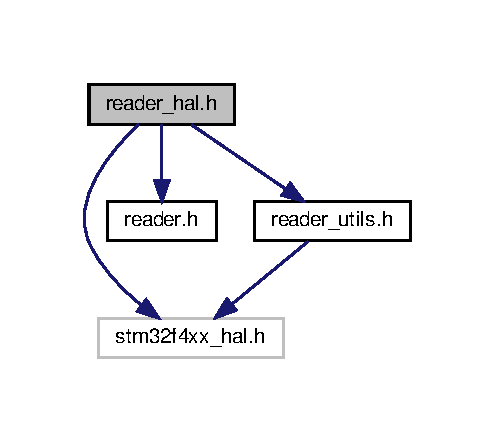
\includegraphics[width=237pt]{reader__hal_8h__incl}
\end{center}
\end{figure}
This graph shows which files directly or indirectly include this file\+:
\nopagebreak
\begin{figure}[H]
\begin{center}
\leavevmode
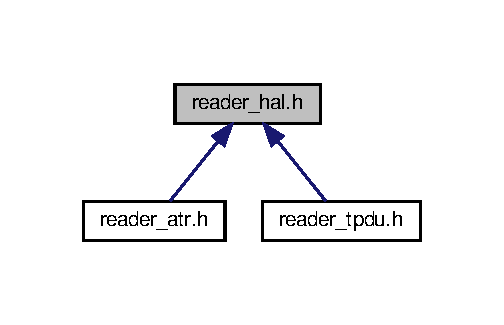
\includegraphics[width=242pt]{reader__hal_8h__dep__incl}
\end{center}
\end{figure}
\subsection*{Macros}
\begin{DoxyCompactItemize}
\item 
\#define \hyperlink{reader__hal_8h_ac771971165e2bc154eeb144c7fec4c9b}{R\+E\+A\+D\+E\+R\+\_\+\+H\+A\+L\+\_\+\+U\+S\+E\+\_\+\+I\+S\+O\+\_\+\+WT}~(uint32\+\_\+t)(0x00000000)
\begin{DoxyCompactList}\small\item\em Valeur permettant d\textquotesingle{}indiquer à uen fonction d\textquotesingle{}envoi/reception que le timeout à appliqué est le WT défini dans la norme I\+SO. \end{DoxyCompactList}\end{DoxyCompactItemize}
\subsection*{Typedefs}
\begin{DoxyCompactItemize}
\item 
typedef enum \hyperlink{reader__hal_8h_a8d3f5996c1f1a9bda2f7f67f84438cdc}{R\+E\+A\+D\+E\+R\+\_\+\+H\+A\+L\+\_\+\+State} \hyperlink{reader__hal_8h_a38d6fedbedcd5c63ef06132db02d5f1c}{R\+E\+A\+D\+E\+R\+\_\+\+H\+A\+L\+\_\+\+State}
\end{DoxyCompactItemize}
\subsection*{Enumerations}
\begin{DoxyCompactItemize}
\item 
enum \hyperlink{reader__hal_8h_a8d3f5996c1f1a9bda2f7f67f84438cdc}{R\+E\+A\+D\+E\+R\+\_\+\+H\+A\+L\+\_\+\+State} \{ \hyperlink{reader__hal_8h_a8d3f5996c1f1a9bda2f7f67f84438cdca4ea3a69a631e49ab11b32e12eadc47e1}{R\+E\+A\+D\+E\+R\+\_\+\+H\+A\+L\+\_\+\+S\+T\+A\+T\+E\+\_\+\+ON} = 1, 
\hyperlink{reader__hal_8h_a8d3f5996c1f1a9bda2f7f67f84438cdca2ad59aa555470a52d3ce37a54e803e38}{R\+E\+A\+D\+E\+R\+\_\+\+H\+A\+L\+\_\+\+S\+T\+A\+T\+E\+\_\+\+O\+FF} = 0
 \}\begin{DoxyCompactList}\small\item\em Type de données permettant d\textquotesingle{}indiquer un état. \end{DoxyCompactList}
\end{DoxyCompactItemize}
\subsection*{Functions}
\begin{DoxyCompactItemize}
\item 
\hyperlink{reader_8h_a2ce152a8d1e28c2847301451aa5bbc20}{R\+E\+A\+D\+E\+R\+\_\+\+Status} \hyperlink{reader__hal_8h_a57e659003860515031408b156696fdce}{R\+E\+A\+D\+E\+R\+\_\+\+H\+A\+L\+\_\+\+Init} (void)
\begin{DoxyCompactList}\small\item\em Fonction pour initialiser la couche d\textquotesingle{}abstraction. \end{DoxyCompactList}\item 
\hyperlink{reader_8h_a2ce152a8d1e28c2847301451aa5bbc20}{R\+E\+A\+D\+E\+R\+\_\+\+Status} \hyperlink{reader__hal_8h_ab5b546fa7480023a33d25c796e31e5f9}{R\+E\+A\+D\+E\+R\+\_\+\+H\+A\+L\+\_\+\+Send\+Char\+Frame} (uint8\+\_\+t $\ast$frame, uint32\+\_\+t frame\+Size, uint32\+\_\+t timeout)
\item 
\hyperlink{reader_8h_a2ce152a8d1e28c2847301451aa5bbc20}{R\+E\+A\+D\+E\+R\+\_\+\+Status} \hyperlink{reader__hal_8h_a07ea773e787d9058fecf1360d5054282}{R\+E\+A\+D\+E\+R\+\_\+\+H\+A\+L\+\_\+\+Rcv\+Char\+Frame} (uint8\+\_\+t $\ast$frame, uint32\+\_\+t frame\+Size, uint32\+\_\+t timeout)
\item 
\hyperlink{reader_8h_a2ce152a8d1e28c2847301451aa5bbc20}{R\+E\+A\+D\+E\+R\+\_\+\+Status} \hyperlink{reader__hal_8h_a2fe91c3405b355d5ac2b24cd66cfe141}{R\+E\+A\+D\+E\+R\+\_\+\+H\+A\+L\+\_\+\+Rcv\+Char} (uint8\+\_\+t $\ast$character, uint32\+\_\+t timeout)
\item 
\hyperlink{reader_8h_a2ce152a8d1e28c2847301451aa5bbc20}{R\+E\+A\+D\+E\+R\+\_\+\+Status} \hyperlink{reader__hal_8h_a55b2435d2d41f1bb9e219ed074d84f66}{R\+E\+A\+D\+E\+R\+\_\+\+H\+A\+L\+\_\+\+Send\+Char} (uint8\+\_\+t character, uint32\+\_\+t timeout)
\item 
\hyperlink{reader_8h_a2ce152a8d1e28c2847301451aa5bbc20}{R\+E\+A\+D\+E\+R\+\_\+\+Status} \hyperlink{reader__hal_8h_a2b4fe7ee983665426f24b4d2ec508886}{R\+E\+A\+D\+E\+R\+\_\+\+H\+A\+L\+\_\+\+Set\+Freq} (uint32\+\_\+t new\+Freq)
\item 
\hyperlink{reader_8h_a2ce152a8d1e28c2847301451aa5bbc20}{R\+E\+A\+D\+E\+R\+\_\+\+Status} \hyperlink{reader__hal_8h_accf05406100c32b0ccfe0a639a3e897b}{R\+E\+A\+D\+E\+R\+\_\+\+H\+A\+L\+\_\+\+Set\+Etu} (uint32\+\_\+t Fi, uint32\+\_\+t Di)
\item 
\hyperlink{reader_8h_a2ce152a8d1e28c2847301451aa5bbc20}{R\+E\+A\+D\+E\+R\+\_\+\+Status} \hyperlink{reader__hal_8h_af7b20bde9d35718e67f0813a48d44b26}{R\+E\+A\+D\+E\+R\+\_\+\+H\+A\+L\+\_\+\+Set\+GT} (uint32\+\_\+t new\+GT)
\item 
\hyperlink{reader_8h_a2ce152a8d1e28c2847301451aa5bbc20}{R\+E\+A\+D\+E\+R\+\_\+\+Status} \hyperlink{reader__hal_8h_aeb464e798a0dbc104147ce3bba2a83d2}{R\+E\+A\+D\+E\+R\+\_\+\+H\+A\+L\+\_\+\+Set\+WT} (uint32\+\_\+t new\+WT)
\item 
\hyperlink{reader_8h_a2ce152a8d1e28c2847301451aa5bbc20}{R\+E\+A\+D\+E\+R\+\_\+\+Status} \hyperlink{reader__hal_8h_a939287b454fa74cad649c7f51972573c}{R\+E\+A\+D\+E\+R\+\_\+\+H\+A\+L\+\_\+\+Set\+Pwr\+Line} (\hyperlink{reader__hal_8h_a8d3f5996c1f1a9bda2f7f67f84438cdc}{R\+E\+A\+D\+E\+R\+\_\+\+H\+A\+L\+\_\+\+State} state)
\item 
\hyperlink{reader_8h_a2ce152a8d1e28c2847301451aa5bbc20}{R\+E\+A\+D\+E\+R\+\_\+\+Status} \hyperlink{reader__hal_8h_aa239fec19d5dbb4d1f33e97d009a298a}{R\+E\+A\+D\+E\+R\+\_\+\+H\+A\+L\+\_\+\+Set\+Rst\+Line} (\hyperlink{reader__hal_8h_a8d3f5996c1f1a9bda2f7f67f84438cdc}{R\+E\+A\+D\+E\+R\+\_\+\+H\+A\+L\+\_\+\+State} state)
\item 
\hyperlink{reader_8h_a2ce152a8d1e28c2847301451aa5bbc20}{R\+E\+A\+D\+E\+R\+\_\+\+Status} \hyperlink{reader__hal_8h_a7800790d0c8f32abbfaf7ac563178aab}{R\+E\+A\+D\+E\+R\+\_\+\+H\+A\+L\+\_\+\+Set\+Clk\+Line} (\hyperlink{reader__hal_8h_a8d3f5996c1f1a9bda2f7f67f84438cdc}{R\+E\+A\+D\+E\+R\+\_\+\+H\+A\+L\+\_\+\+State} state)
\item 
\hyperlink{reader_8h_a2ce152a8d1e28c2847301451aa5bbc20}{R\+E\+A\+D\+E\+R\+\_\+\+Status} \hyperlink{reader__hal_8h_a028de7447c509728ea49fcc17645f4ad}{R\+E\+A\+D\+E\+R\+\_\+\+H\+A\+L\+\_\+\+Set\+I\+O\+Line} (\hyperlink{reader__hal_8h_a8d3f5996c1f1a9bda2f7f67f84438cdc}{R\+E\+A\+D\+E\+R\+\_\+\+H\+A\+L\+\_\+\+State} state)
\item 
void \hyperlink{reader__hal_8h_a3eef81d5258fc6f5bae109fe98196dba}{R\+E\+A\+D\+E\+R\+\_\+\+H\+A\+L\+\_\+\+Delay} (uint32\+\_\+t t\+Mili)
\item 
void \hyperlink{reader__hal_8h_a6654c9550b24f4bf395c97bbc3b18304}{R\+E\+A\+D\+E\+R\+\_\+\+H\+A\+L\+\_\+\+Err\+Handler} (void)
\end{DoxyCompactItemize}


\subsection{Detailed Description}
Prototypes de la couche d\textquotesingle{}abstraction. 

\begin{DoxyAuthor}{Author}
B. Simunovic 
\end{DoxyAuthor}
\begin{DoxyDate}{Date}
28 mars 2018
\end{DoxyDate}
Dans ce fichier son définis les prototypes de fonctions de la couche d\textquotesingle{}abstraction du matériel du lecteur. 

\subsection{Macro Definition Documentation}
\mbox{\Hypertarget{reader__hal_8h_ac771971165e2bc154eeb144c7fec4c9b}\label{reader__hal_8h_ac771971165e2bc154eeb144c7fec4c9b}} 
\index{reader\+\_\+hal.\+h@{reader\+\_\+hal.\+h}!R\+E\+A\+D\+E\+R\+\_\+\+H\+A\+L\+\_\+\+U\+S\+E\+\_\+\+I\+S\+O\+\_\+\+WT@{R\+E\+A\+D\+E\+R\+\_\+\+H\+A\+L\+\_\+\+U\+S\+E\+\_\+\+I\+S\+O\+\_\+\+WT}}
\index{R\+E\+A\+D\+E\+R\+\_\+\+H\+A\+L\+\_\+\+U\+S\+E\+\_\+\+I\+S\+O\+\_\+\+WT@{R\+E\+A\+D\+E\+R\+\_\+\+H\+A\+L\+\_\+\+U\+S\+E\+\_\+\+I\+S\+O\+\_\+\+WT}!reader\+\_\+hal.\+h@{reader\+\_\+hal.\+h}}
\subsubsection{\texorpdfstring{R\+E\+A\+D\+E\+R\+\_\+\+H\+A\+L\+\_\+\+U\+S\+E\+\_\+\+I\+S\+O\+\_\+\+WT}{READER\_HAL\_USE\_ISO\_WT}}
{\footnotesize\ttfamily \#define R\+E\+A\+D\+E\+R\+\_\+\+H\+A\+L\+\_\+\+U\+S\+E\+\_\+\+I\+S\+O\+\_\+\+WT~(uint32\+\_\+t)(0x00000000)}



Valeur permettant d\textquotesingle{}indiquer à uen fonction d\textquotesingle{}envoi/reception que le timeout à appliqué est le WT défini dans la norme I\+SO. 

Cette constante passée en parametre à certaines fonctions d\textquotesingle{}envoi et de réception permet d\textquotesingle{}indiquer le type de timeout à utiliser. Si la valeur de timeout passée en argument à une fonction d\textquotesingle{}envoi/réception est différente de R\+E\+A\+D\+E\+R\+\_\+\+H\+A\+L\+\_\+\+U\+S\+E\+\_\+\+I\+S\+O\+\_\+\+WT alors le timout appliqué sera cette valeur en milisecondes. Si la valeur de timeout passée en argument à une fonction d\textquotesingle{}envoi/réception est R\+E\+A\+D\+E\+R\+\_\+\+H\+A\+L\+\_\+\+U\+S\+E\+\_\+\+I\+S\+O\+\_\+\+WT alors le timeout appliqué sera le \char`\"{}wait time\char`\"{} (WT) tel que défini dans la norme I\+SO. 

\subsection{Typedef Documentation}
\mbox{\Hypertarget{reader__hal_8h_a38d6fedbedcd5c63ef06132db02d5f1c}\label{reader__hal_8h_a38d6fedbedcd5c63ef06132db02d5f1c}} 
\index{reader\+\_\+hal.\+h@{reader\+\_\+hal.\+h}!R\+E\+A\+D\+E\+R\+\_\+\+H\+A\+L\+\_\+\+State@{R\+E\+A\+D\+E\+R\+\_\+\+H\+A\+L\+\_\+\+State}}
\index{R\+E\+A\+D\+E\+R\+\_\+\+H\+A\+L\+\_\+\+State@{R\+E\+A\+D\+E\+R\+\_\+\+H\+A\+L\+\_\+\+State}!reader\+\_\+hal.\+h@{reader\+\_\+hal.\+h}}
\subsubsection{\texorpdfstring{R\+E\+A\+D\+E\+R\+\_\+\+H\+A\+L\+\_\+\+State}{READER\_HAL\_State}}
{\footnotesize\ttfamily typedef enum \hyperlink{reader__hal_8h_a8d3f5996c1f1a9bda2f7f67f84438cdc}{R\+E\+A\+D\+E\+R\+\_\+\+H\+A\+L\+\_\+\+State} \hyperlink{reader__hal_8h_a8d3f5996c1f1a9bda2f7f67f84438cdc}{R\+E\+A\+D\+E\+R\+\_\+\+H\+A\+L\+\_\+\+State}}



\subsection{Enumeration Type Documentation}
\mbox{\Hypertarget{reader__hal_8h_a8d3f5996c1f1a9bda2f7f67f84438cdc}\label{reader__hal_8h_a8d3f5996c1f1a9bda2f7f67f84438cdc}} 
\index{reader\+\_\+hal.\+h@{reader\+\_\+hal.\+h}!R\+E\+A\+D\+E\+R\+\_\+\+H\+A\+L\+\_\+\+State@{R\+E\+A\+D\+E\+R\+\_\+\+H\+A\+L\+\_\+\+State}}
\index{R\+E\+A\+D\+E\+R\+\_\+\+H\+A\+L\+\_\+\+State@{R\+E\+A\+D\+E\+R\+\_\+\+H\+A\+L\+\_\+\+State}!reader\+\_\+hal.\+h@{reader\+\_\+hal.\+h}}
\subsubsection{\texorpdfstring{R\+E\+A\+D\+E\+R\+\_\+\+H\+A\+L\+\_\+\+State}{READER\_HAL\_State}}
{\footnotesize\ttfamily enum \hyperlink{reader__hal_8h_a8d3f5996c1f1a9bda2f7f67f84438cdc}{R\+E\+A\+D\+E\+R\+\_\+\+H\+A\+L\+\_\+\+State}}



Type de données permettant d\textquotesingle{}indiquer un état. 

\begin{DoxyEnumFields}{Enumerator}
\raisebox{\heightof{T}}[0pt][0pt]{\index{R\+E\+A\+D\+E\+R\+\_\+\+H\+A\+L\+\_\+\+S\+T\+A\+T\+E\+\_\+\+ON@{R\+E\+A\+D\+E\+R\+\_\+\+H\+A\+L\+\_\+\+S\+T\+A\+T\+E\+\_\+\+ON}!reader\+\_\+hal.\+h@{reader\+\_\+hal.\+h}}\index{reader\+\_\+hal.\+h@{reader\+\_\+hal.\+h}!R\+E\+A\+D\+E\+R\+\_\+\+H\+A\+L\+\_\+\+S\+T\+A\+T\+E\+\_\+\+ON@{R\+E\+A\+D\+E\+R\+\_\+\+H\+A\+L\+\_\+\+S\+T\+A\+T\+E\+\_\+\+ON}}}\mbox{\Hypertarget{reader__hal_8h_a8d3f5996c1f1a9bda2f7f67f84438cdca4ea3a69a631e49ab11b32e12eadc47e1}\label{reader__hal_8h_a8d3f5996c1f1a9bda2f7f67f84438cdca4ea3a69a631e49ab11b32e12eadc47e1}} 
R\+E\+A\+D\+E\+R\+\_\+\+H\+A\+L\+\_\+\+S\+T\+A\+T\+E\+\_\+\+ON&\\
\hline

\raisebox{\heightof{T}}[0pt][0pt]{\index{R\+E\+A\+D\+E\+R\+\_\+\+H\+A\+L\+\_\+\+S\+T\+A\+T\+E\+\_\+\+O\+FF@{R\+E\+A\+D\+E\+R\+\_\+\+H\+A\+L\+\_\+\+S\+T\+A\+T\+E\+\_\+\+O\+FF}!reader\+\_\+hal.\+h@{reader\+\_\+hal.\+h}}\index{reader\+\_\+hal.\+h@{reader\+\_\+hal.\+h}!R\+E\+A\+D\+E\+R\+\_\+\+H\+A\+L\+\_\+\+S\+T\+A\+T\+E\+\_\+\+O\+FF@{R\+E\+A\+D\+E\+R\+\_\+\+H\+A\+L\+\_\+\+S\+T\+A\+T\+E\+\_\+\+O\+FF}}}\mbox{\Hypertarget{reader__hal_8h_a8d3f5996c1f1a9bda2f7f67f84438cdca2ad59aa555470a52d3ce37a54e803e38}\label{reader__hal_8h_a8d3f5996c1f1a9bda2f7f67f84438cdca2ad59aa555470a52d3ce37a54e803e38}} 
R\+E\+A\+D\+E\+R\+\_\+\+H\+A\+L\+\_\+\+S\+T\+A\+T\+E\+\_\+\+O\+FF&\\
\hline

\end{DoxyEnumFields}


\subsection{Function Documentation}
\mbox{\Hypertarget{reader__hal_8h_a3eef81d5258fc6f5bae109fe98196dba}\label{reader__hal_8h_a3eef81d5258fc6f5bae109fe98196dba}} 
\index{reader\+\_\+hal.\+h@{reader\+\_\+hal.\+h}!R\+E\+A\+D\+E\+R\+\_\+\+H\+A\+L\+\_\+\+Delay@{R\+E\+A\+D\+E\+R\+\_\+\+H\+A\+L\+\_\+\+Delay}}
\index{R\+E\+A\+D\+E\+R\+\_\+\+H\+A\+L\+\_\+\+Delay@{R\+E\+A\+D\+E\+R\+\_\+\+H\+A\+L\+\_\+\+Delay}!reader\+\_\+hal.\+h@{reader\+\_\+hal.\+h}}
\subsubsection{\texorpdfstring{R\+E\+A\+D\+E\+R\+\_\+\+H\+A\+L\+\_\+\+Delay()}{READER\_HAL\_Delay()}}
{\footnotesize\ttfamily void R\+E\+A\+D\+E\+R\+\_\+\+H\+A\+L\+\_\+\+Delay (\begin{DoxyParamCaption}\item[{uint32\+\_\+t}]{t\+Mili }\end{DoxyParamCaption})}

\mbox{\Hypertarget{reader__hal_8h_a6654c9550b24f4bf395c97bbc3b18304}\label{reader__hal_8h_a6654c9550b24f4bf395c97bbc3b18304}} 
\index{reader\+\_\+hal.\+h@{reader\+\_\+hal.\+h}!R\+E\+A\+D\+E\+R\+\_\+\+H\+A\+L\+\_\+\+Err\+Handler@{R\+E\+A\+D\+E\+R\+\_\+\+H\+A\+L\+\_\+\+Err\+Handler}}
\index{R\+E\+A\+D\+E\+R\+\_\+\+H\+A\+L\+\_\+\+Err\+Handler@{R\+E\+A\+D\+E\+R\+\_\+\+H\+A\+L\+\_\+\+Err\+Handler}!reader\+\_\+hal.\+h@{reader\+\_\+hal.\+h}}
\subsubsection{\texorpdfstring{R\+E\+A\+D\+E\+R\+\_\+\+H\+A\+L\+\_\+\+Err\+Handler()}{READER\_HAL\_ErrHandler()}}
{\footnotesize\ttfamily void R\+E\+A\+D\+E\+R\+\_\+\+H\+A\+L\+\_\+\+Err\+Handler (\begin{DoxyParamCaption}\item[{void}]{ }\end{DoxyParamCaption})}

\mbox{\Hypertarget{reader__hal_8h_a57e659003860515031408b156696fdce}\label{reader__hal_8h_a57e659003860515031408b156696fdce}} 
\index{reader\+\_\+hal.\+h@{reader\+\_\+hal.\+h}!R\+E\+A\+D\+E\+R\+\_\+\+H\+A\+L\+\_\+\+Init@{R\+E\+A\+D\+E\+R\+\_\+\+H\+A\+L\+\_\+\+Init}}
\index{R\+E\+A\+D\+E\+R\+\_\+\+H\+A\+L\+\_\+\+Init@{R\+E\+A\+D\+E\+R\+\_\+\+H\+A\+L\+\_\+\+Init}!reader\+\_\+hal.\+h@{reader\+\_\+hal.\+h}}
\subsubsection{\texorpdfstring{R\+E\+A\+D\+E\+R\+\_\+\+H\+A\+L\+\_\+\+Init()}{READER\_HAL\_Init()}}
{\footnotesize\ttfamily \hyperlink{reader_8h_a2ce152a8d1e28c2847301451aa5bbc20}{R\+E\+A\+D\+E\+R\+\_\+\+Status} R\+E\+A\+D\+E\+R\+\_\+\+H\+A\+L\+\_\+\+Init (\begin{DoxyParamCaption}\item[{void}]{ }\end{DoxyParamCaption})}



Fonction pour initialiser la couche d\textquotesingle{}abstraction. 

\begin{DoxyReturn}{Returns}
Valeur de type R\+E\+A\+D\+E\+R\+\_\+\+Status. R\+E\+A\+D\+E\+R\+\_\+\+OK si l\textquotesingle{}exécution s\textquotesingle{}est correctement déroulée. R\+E\+A\+D\+E\+R\+\_\+\+NO dans le cas contraire. 
\end{DoxyReturn}
\mbox{\Hypertarget{reader__hal_8h_a2fe91c3405b355d5ac2b24cd66cfe141}\label{reader__hal_8h_a2fe91c3405b355d5ac2b24cd66cfe141}} 
\index{reader\+\_\+hal.\+h@{reader\+\_\+hal.\+h}!R\+E\+A\+D\+E\+R\+\_\+\+H\+A\+L\+\_\+\+Rcv\+Char@{R\+E\+A\+D\+E\+R\+\_\+\+H\+A\+L\+\_\+\+Rcv\+Char}}
\index{R\+E\+A\+D\+E\+R\+\_\+\+H\+A\+L\+\_\+\+Rcv\+Char@{R\+E\+A\+D\+E\+R\+\_\+\+H\+A\+L\+\_\+\+Rcv\+Char}!reader\+\_\+hal.\+h@{reader\+\_\+hal.\+h}}
\subsubsection{\texorpdfstring{R\+E\+A\+D\+E\+R\+\_\+\+H\+A\+L\+\_\+\+Rcv\+Char()}{READER\_HAL\_RcvChar()}}
{\footnotesize\ttfamily \hyperlink{reader_8h_a2ce152a8d1e28c2847301451aa5bbc20}{R\+E\+A\+D\+E\+R\+\_\+\+Status} R\+E\+A\+D\+E\+R\+\_\+\+H\+A\+L\+\_\+\+Rcv\+Char (\begin{DoxyParamCaption}\item[{uint8\+\_\+t $\ast$}]{character,  }\item[{uint32\+\_\+t}]{timeout }\end{DoxyParamCaption})}

\mbox{\Hypertarget{reader__hal_8h_a07ea773e787d9058fecf1360d5054282}\label{reader__hal_8h_a07ea773e787d9058fecf1360d5054282}} 
\index{reader\+\_\+hal.\+h@{reader\+\_\+hal.\+h}!R\+E\+A\+D\+E\+R\+\_\+\+H\+A\+L\+\_\+\+Rcv\+Char\+Frame@{R\+E\+A\+D\+E\+R\+\_\+\+H\+A\+L\+\_\+\+Rcv\+Char\+Frame}}
\index{R\+E\+A\+D\+E\+R\+\_\+\+H\+A\+L\+\_\+\+Rcv\+Char\+Frame@{R\+E\+A\+D\+E\+R\+\_\+\+H\+A\+L\+\_\+\+Rcv\+Char\+Frame}!reader\+\_\+hal.\+h@{reader\+\_\+hal.\+h}}
\subsubsection{\texorpdfstring{R\+E\+A\+D\+E\+R\+\_\+\+H\+A\+L\+\_\+\+Rcv\+Char\+Frame()}{READER\_HAL\_RcvCharFrame()}}
{\footnotesize\ttfamily \hyperlink{reader_8h_a2ce152a8d1e28c2847301451aa5bbc20}{R\+E\+A\+D\+E\+R\+\_\+\+Status} R\+E\+A\+D\+E\+R\+\_\+\+H\+A\+L\+\_\+\+Rcv\+Char\+Frame (\begin{DoxyParamCaption}\item[{uint8\+\_\+t $\ast$}]{frame,  }\item[{uint32\+\_\+t}]{frame\+Size,  }\item[{uint32\+\_\+t}]{timeout }\end{DoxyParamCaption})}

\mbox{\Hypertarget{reader__hal_8h_a55b2435d2d41f1bb9e219ed074d84f66}\label{reader__hal_8h_a55b2435d2d41f1bb9e219ed074d84f66}} 
\index{reader\+\_\+hal.\+h@{reader\+\_\+hal.\+h}!R\+E\+A\+D\+E\+R\+\_\+\+H\+A\+L\+\_\+\+Send\+Char@{R\+E\+A\+D\+E\+R\+\_\+\+H\+A\+L\+\_\+\+Send\+Char}}
\index{R\+E\+A\+D\+E\+R\+\_\+\+H\+A\+L\+\_\+\+Send\+Char@{R\+E\+A\+D\+E\+R\+\_\+\+H\+A\+L\+\_\+\+Send\+Char}!reader\+\_\+hal.\+h@{reader\+\_\+hal.\+h}}
\subsubsection{\texorpdfstring{R\+E\+A\+D\+E\+R\+\_\+\+H\+A\+L\+\_\+\+Send\+Char()}{READER\_HAL\_SendChar()}}
{\footnotesize\ttfamily \hyperlink{reader_8h_a2ce152a8d1e28c2847301451aa5bbc20}{R\+E\+A\+D\+E\+R\+\_\+\+Status} R\+E\+A\+D\+E\+R\+\_\+\+H\+A\+L\+\_\+\+Send\+Char (\begin{DoxyParamCaption}\item[{uint8\+\_\+t}]{character,  }\item[{uint32\+\_\+t}]{timeout }\end{DoxyParamCaption})}

\mbox{\Hypertarget{reader__hal_8h_ab5b546fa7480023a33d25c796e31e5f9}\label{reader__hal_8h_ab5b546fa7480023a33d25c796e31e5f9}} 
\index{reader\+\_\+hal.\+h@{reader\+\_\+hal.\+h}!R\+E\+A\+D\+E\+R\+\_\+\+H\+A\+L\+\_\+\+Send\+Char\+Frame@{R\+E\+A\+D\+E\+R\+\_\+\+H\+A\+L\+\_\+\+Send\+Char\+Frame}}
\index{R\+E\+A\+D\+E\+R\+\_\+\+H\+A\+L\+\_\+\+Send\+Char\+Frame@{R\+E\+A\+D\+E\+R\+\_\+\+H\+A\+L\+\_\+\+Send\+Char\+Frame}!reader\+\_\+hal.\+h@{reader\+\_\+hal.\+h}}
\subsubsection{\texorpdfstring{R\+E\+A\+D\+E\+R\+\_\+\+H\+A\+L\+\_\+\+Send\+Char\+Frame()}{READER\_HAL\_SendCharFrame()}}
{\footnotesize\ttfamily \hyperlink{reader_8h_a2ce152a8d1e28c2847301451aa5bbc20}{R\+E\+A\+D\+E\+R\+\_\+\+Status} R\+E\+A\+D\+E\+R\+\_\+\+H\+A\+L\+\_\+\+Send\+Char\+Frame (\begin{DoxyParamCaption}\item[{uint8\+\_\+t $\ast$}]{frame,  }\item[{uint32\+\_\+t}]{frame\+Size,  }\item[{uint32\+\_\+t}]{timeout }\end{DoxyParamCaption})}

\mbox{\Hypertarget{reader__hal_8h_a7800790d0c8f32abbfaf7ac563178aab}\label{reader__hal_8h_a7800790d0c8f32abbfaf7ac563178aab}} 
\index{reader\+\_\+hal.\+h@{reader\+\_\+hal.\+h}!R\+E\+A\+D\+E\+R\+\_\+\+H\+A\+L\+\_\+\+Set\+Clk\+Line@{R\+E\+A\+D\+E\+R\+\_\+\+H\+A\+L\+\_\+\+Set\+Clk\+Line}}
\index{R\+E\+A\+D\+E\+R\+\_\+\+H\+A\+L\+\_\+\+Set\+Clk\+Line@{R\+E\+A\+D\+E\+R\+\_\+\+H\+A\+L\+\_\+\+Set\+Clk\+Line}!reader\+\_\+hal.\+h@{reader\+\_\+hal.\+h}}
\subsubsection{\texorpdfstring{R\+E\+A\+D\+E\+R\+\_\+\+H\+A\+L\+\_\+\+Set\+Clk\+Line()}{READER\_HAL\_SetClkLine()}}
{\footnotesize\ttfamily \hyperlink{reader_8h_a2ce152a8d1e28c2847301451aa5bbc20}{R\+E\+A\+D\+E\+R\+\_\+\+Status} R\+E\+A\+D\+E\+R\+\_\+\+H\+A\+L\+\_\+\+Set\+Clk\+Line (\begin{DoxyParamCaption}\item[{\hyperlink{reader__hal_8h_a8d3f5996c1f1a9bda2f7f67f84438cdc}{R\+E\+A\+D\+E\+R\+\_\+\+H\+A\+L\+\_\+\+State}}]{state }\end{DoxyParamCaption})}

\mbox{\Hypertarget{reader__hal_8h_accf05406100c32b0ccfe0a639a3e897b}\label{reader__hal_8h_accf05406100c32b0ccfe0a639a3e897b}} 
\index{reader\+\_\+hal.\+h@{reader\+\_\+hal.\+h}!R\+E\+A\+D\+E\+R\+\_\+\+H\+A\+L\+\_\+\+Set\+Etu@{R\+E\+A\+D\+E\+R\+\_\+\+H\+A\+L\+\_\+\+Set\+Etu}}
\index{R\+E\+A\+D\+E\+R\+\_\+\+H\+A\+L\+\_\+\+Set\+Etu@{R\+E\+A\+D\+E\+R\+\_\+\+H\+A\+L\+\_\+\+Set\+Etu}!reader\+\_\+hal.\+h@{reader\+\_\+hal.\+h}}
\subsubsection{\texorpdfstring{R\+E\+A\+D\+E\+R\+\_\+\+H\+A\+L\+\_\+\+Set\+Etu()}{READER\_HAL\_SetEtu()}}
{\footnotesize\ttfamily \hyperlink{reader_8h_a2ce152a8d1e28c2847301451aa5bbc20}{R\+E\+A\+D\+E\+R\+\_\+\+Status} R\+E\+A\+D\+E\+R\+\_\+\+H\+A\+L\+\_\+\+Set\+Etu (\begin{DoxyParamCaption}\item[{uint32\+\_\+t}]{Fi,  }\item[{uint32\+\_\+t}]{Di }\end{DoxyParamCaption})}

\mbox{\Hypertarget{reader__hal_8h_a2b4fe7ee983665426f24b4d2ec508886}\label{reader__hal_8h_a2b4fe7ee983665426f24b4d2ec508886}} 
\index{reader\+\_\+hal.\+h@{reader\+\_\+hal.\+h}!R\+E\+A\+D\+E\+R\+\_\+\+H\+A\+L\+\_\+\+Set\+Freq@{R\+E\+A\+D\+E\+R\+\_\+\+H\+A\+L\+\_\+\+Set\+Freq}}
\index{R\+E\+A\+D\+E\+R\+\_\+\+H\+A\+L\+\_\+\+Set\+Freq@{R\+E\+A\+D\+E\+R\+\_\+\+H\+A\+L\+\_\+\+Set\+Freq}!reader\+\_\+hal.\+h@{reader\+\_\+hal.\+h}}
\subsubsection{\texorpdfstring{R\+E\+A\+D\+E\+R\+\_\+\+H\+A\+L\+\_\+\+Set\+Freq()}{READER\_HAL\_SetFreq()}}
{\footnotesize\ttfamily \hyperlink{reader_8h_a2ce152a8d1e28c2847301451aa5bbc20}{R\+E\+A\+D\+E\+R\+\_\+\+Status} R\+E\+A\+D\+E\+R\+\_\+\+H\+A\+L\+\_\+\+Set\+Freq (\begin{DoxyParamCaption}\item[{uint32\+\_\+t}]{new\+Freq }\end{DoxyParamCaption})}

\mbox{\Hypertarget{reader__hal_8h_af7b20bde9d35718e67f0813a48d44b26}\label{reader__hal_8h_af7b20bde9d35718e67f0813a48d44b26}} 
\index{reader\+\_\+hal.\+h@{reader\+\_\+hal.\+h}!R\+E\+A\+D\+E\+R\+\_\+\+H\+A\+L\+\_\+\+Set\+GT@{R\+E\+A\+D\+E\+R\+\_\+\+H\+A\+L\+\_\+\+Set\+GT}}
\index{R\+E\+A\+D\+E\+R\+\_\+\+H\+A\+L\+\_\+\+Set\+GT@{R\+E\+A\+D\+E\+R\+\_\+\+H\+A\+L\+\_\+\+Set\+GT}!reader\+\_\+hal.\+h@{reader\+\_\+hal.\+h}}
\subsubsection{\texorpdfstring{R\+E\+A\+D\+E\+R\+\_\+\+H\+A\+L\+\_\+\+Set\+G\+T()}{READER\_HAL\_SetGT()}}
{\footnotesize\ttfamily \hyperlink{reader_8h_a2ce152a8d1e28c2847301451aa5bbc20}{R\+E\+A\+D\+E\+R\+\_\+\+Status} R\+E\+A\+D\+E\+R\+\_\+\+H\+A\+L\+\_\+\+Set\+GT (\begin{DoxyParamCaption}\item[{uint32\+\_\+t}]{new\+GT }\end{DoxyParamCaption})}

\mbox{\Hypertarget{reader__hal_8h_a028de7447c509728ea49fcc17645f4ad}\label{reader__hal_8h_a028de7447c509728ea49fcc17645f4ad}} 
\index{reader\+\_\+hal.\+h@{reader\+\_\+hal.\+h}!R\+E\+A\+D\+E\+R\+\_\+\+H\+A\+L\+\_\+\+Set\+I\+O\+Line@{R\+E\+A\+D\+E\+R\+\_\+\+H\+A\+L\+\_\+\+Set\+I\+O\+Line}}
\index{R\+E\+A\+D\+E\+R\+\_\+\+H\+A\+L\+\_\+\+Set\+I\+O\+Line@{R\+E\+A\+D\+E\+R\+\_\+\+H\+A\+L\+\_\+\+Set\+I\+O\+Line}!reader\+\_\+hal.\+h@{reader\+\_\+hal.\+h}}
\subsubsection{\texorpdfstring{R\+E\+A\+D\+E\+R\+\_\+\+H\+A\+L\+\_\+\+Set\+I\+O\+Line()}{READER\_HAL\_SetIOLine()}}
{\footnotesize\ttfamily \hyperlink{reader_8h_a2ce152a8d1e28c2847301451aa5bbc20}{R\+E\+A\+D\+E\+R\+\_\+\+Status} R\+E\+A\+D\+E\+R\+\_\+\+H\+A\+L\+\_\+\+Set\+I\+O\+Line (\begin{DoxyParamCaption}\item[{\hyperlink{reader__hal_8h_a8d3f5996c1f1a9bda2f7f67f84438cdc}{R\+E\+A\+D\+E\+R\+\_\+\+H\+A\+L\+\_\+\+State}}]{state }\end{DoxyParamCaption})}

\mbox{\Hypertarget{reader__hal_8h_a939287b454fa74cad649c7f51972573c}\label{reader__hal_8h_a939287b454fa74cad649c7f51972573c}} 
\index{reader\+\_\+hal.\+h@{reader\+\_\+hal.\+h}!R\+E\+A\+D\+E\+R\+\_\+\+H\+A\+L\+\_\+\+Set\+Pwr\+Line@{R\+E\+A\+D\+E\+R\+\_\+\+H\+A\+L\+\_\+\+Set\+Pwr\+Line}}
\index{R\+E\+A\+D\+E\+R\+\_\+\+H\+A\+L\+\_\+\+Set\+Pwr\+Line@{R\+E\+A\+D\+E\+R\+\_\+\+H\+A\+L\+\_\+\+Set\+Pwr\+Line}!reader\+\_\+hal.\+h@{reader\+\_\+hal.\+h}}
\subsubsection{\texorpdfstring{R\+E\+A\+D\+E\+R\+\_\+\+H\+A\+L\+\_\+\+Set\+Pwr\+Line()}{READER\_HAL\_SetPwrLine()}}
{\footnotesize\ttfamily \hyperlink{reader_8h_a2ce152a8d1e28c2847301451aa5bbc20}{R\+E\+A\+D\+E\+R\+\_\+\+Status} R\+E\+A\+D\+E\+R\+\_\+\+H\+A\+L\+\_\+\+Set\+Pwr\+Line (\begin{DoxyParamCaption}\item[{\hyperlink{reader__hal_8h_a8d3f5996c1f1a9bda2f7f67f84438cdc}{R\+E\+A\+D\+E\+R\+\_\+\+H\+A\+L\+\_\+\+State}}]{state }\end{DoxyParamCaption})}

\mbox{\Hypertarget{reader__hal_8h_aa239fec19d5dbb4d1f33e97d009a298a}\label{reader__hal_8h_aa239fec19d5dbb4d1f33e97d009a298a}} 
\index{reader\+\_\+hal.\+h@{reader\+\_\+hal.\+h}!R\+E\+A\+D\+E\+R\+\_\+\+H\+A\+L\+\_\+\+Set\+Rst\+Line@{R\+E\+A\+D\+E\+R\+\_\+\+H\+A\+L\+\_\+\+Set\+Rst\+Line}}
\index{R\+E\+A\+D\+E\+R\+\_\+\+H\+A\+L\+\_\+\+Set\+Rst\+Line@{R\+E\+A\+D\+E\+R\+\_\+\+H\+A\+L\+\_\+\+Set\+Rst\+Line}!reader\+\_\+hal.\+h@{reader\+\_\+hal.\+h}}
\subsubsection{\texorpdfstring{R\+E\+A\+D\+E\+R\+\_\+\+H\+A\+L\+\_\+\+Set\+Rst\+Line()}{READER\_HAL\_SetRstLine()}}
{\footnotesize\ttfamily \hyperlink{reader_8h_a2ce152a8d1e28c2847301451aa5bbc20}{R\+E\+A\+D\+E\+R\+\_\+\+Status} R\+E\+A\+D\+E\+R\+\_\+\+H\+A\+L\+\_\+\+Set\+Rst\+Line (\begin{DoxyParamCaption}\item[{\hyperlink{reader__hal_8h_a8d3f5996c1f1a9bda2f7f67f84438cdc}{R\+E\+A\+D\+E\+R\+\_\+\+H\+A\+L\+\_\+\+State}}]{state }\end{DoxyParamCaption})}

\mbox{\Hypertarget{reader__hal_8h_aeb464e798a0dbc104147ce3bba2a83d2}\label{reader__hal_8h_aeb464e798a0dbc104147ce3bba2a83d2}} 
\index{reader\+\_\+hal.\+h@{reader\+\_\+hal.\+h}!R\+E\+A\+D\+E\+R\+\_\+\+H\+A\+L\+\_\+\+Set\+WT@{R\+E\+A\+D\+E\+R\+\_\+\+H\+A\+L\+\_\+\+Set\+WT}}
\index{R\+E\+A\+D\+E\+R\+\_\+\+H\+A\+L\+\_\+\+Set\+WT@{R\+E\+A\+D\+E\+R\+\_\+\+H\+A\+L\+\_\+\+Set\+WT}!reader\+\_\+hal.\+h@{reader\+\_\+hal.\+h}}
\subsubsection{\texorpdfstring{R\+E\+A\+D\+E\+R\+\_\+\+H\+A\+L\+\_\+\+Set\+W\+T()}{READER\_HAL\_SetWT()}}
{\footnotesize\ttfamily \hyperlink{reader_8h_a2ce152a8d1e28c2847301451aa5bbc20}{R\+E\+A\+D\+E\+R\+\_\+\+Status} R\+E\+A\+D\+E\+R\+\_\+\+H\+A\+L\+\_\+\+Set\+WT (\begin{DoxyParamCaption}\item[{uint32\+\_\+t}]{new\+WT }\end{DoxyParamCaption})}


\hypertarget{reader__periph_8h}{}\section{reader\+\_\+periph.\+h File Reference}
\label{reader__periph_8h}\index{reader\+\_\+periph.\+h@{reader\+\_\+periph.\+h}}
{\ttfamily \#include \char`\"{}stm32f4xx\+\_\+hal.\+h\char`\"{}}\newline
{\ttfamily \#include \char`\"{}reader\+\_\+utils.\+h\char`\"{}}\newline
{\ttfamily \#include \char`\"{}reader.\+h\char`\"{}}\newline
Include dependency graph for reader\+\_\+periph.\+h\+:
\nopagebreak
\begin{figure}[H]
\begin{center}
\leavevmode
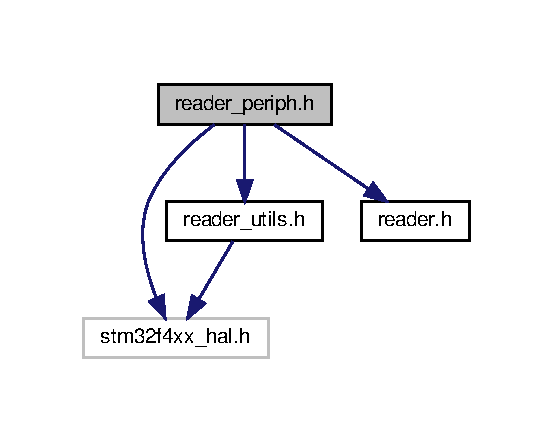
\includegraphics[width=266pt]{reader__periph_8h__incl}
\end{center}
\end{figure}
\subsection*{Macros}
\begin{DoxyCompactItemize}
\item 
\#define \hyperlink{reader__periph_8h_a317b1bc1e6cbcfd98dc6a58a02465ac7}{R\+E\+A\+D\+E\+R\+\_\+\+P\+E\+R\+I\+P\+H\+\_\+\+C\+L\+K\+\_\+\+P\+IN}~G\+P\+I\+O\+\_\+\+P\+I\+N\+\_\+4
\item 
\#define \hyperlink{reader__periph_8h_ad0d1949acfe0d6850dfdd2acc9ba91eb}{R\+E\+A\+D\+E\+R\+\_\+\+P\+E\+R\+I\+P\+H\+\_\+\+I\+O\+\_\+\+P\+IN}~G\+P\+I\+O\+\_\+\+P\+I\+N\+\_\+2
\item 
\#define \hyperlink{reader__periph_8h_a8e314b00e4e07cc18ae17c38fb666bae}{R\+E\+A\+D\+E\+R\+\_\+\+P\+E\+R\+I\+P\+H\+\_\+\+R\+S\+T\+\_\+\+P\+IN}~G\+P\+I\+O\+\_\+\+P\+I\+N\+\_\+5
\item 
\#define \hyperlink{reader__periph_8h_a789a2761608f50e1cdfb5f89f9f49f37}{R\+E\+A\+D\+E\+R\+\_\+\+P\+E\+R\+I\+P\+H\+\_\+\+P\+W\+R\+\_\+\+P\+IN}~G\+P\+I\+O\+\_\+\+P\+I\+N\+\_\+6
\item 
\#define \hyperlink{reader__periph_8h_a8c27fcb23428fc0b6a2452ca8f7e9690}{R\+E\+A\+D\+E\+R\+\_\+\+P\+E\+R\+I\+P\+H\+\_\+\+C\+L\+K\+\_\+\+P\+O\+RT}~G\+P\+I\+OA
\item 
\#define \hyperlink{reader__periph_8h_a6232b2db45df76299d0ab8da77eaf8c8}{R\+E\+A\+D\+E\+R\+\_\+\+P\+E\+R\+I\+P\+H\+\_\+\+I\+O\+\_\+\+P\+O\+RT}~G\+P\+I\+OA
\item 
\#define \hyperlink{reader__periph_8h_a05fdbada53b8e75e2edd99262f6d5a72}{R\+E\+A\+D\+E\+R\+\_\+\+P\+E\+R\+I\+P\+H\+\_\+\+R\+S\+T\+\_\+\+P\+O\+RT}~G\+P\+I\+OA
\item 
\#define \hyperlink{reader__periph_8h_a7851cb5da388105521c325e7c7705cb9}{R\+E\+A\+D\+E\+R\+\_\+\+P\+E\+R\+I\+P\+H\+\_\+\+P\+W\+R\+\_\+\+P\+O\+RT}~G\+P\+I\+OA
\end{DoxyCompactItemize}
\subsection*{Typedefs}
\begin{DoxyCompactItemize}
\item 
typedef enum \hyperlink{reader__periph_8h_a98502b203c0e3b96beb76608e52b9f61}{R\+E\+A\+D\+E\+R\+\_\+\+P\+E\+R\+I\+P\+H\+\_\+\+Status} \hyperlink{reader__periph_8h_aa28804bba57a159183a87ff813aabb06}{R\+E\+A\+D\+E\+R\+\_\+\+P\+E\+R\+I\+P\+H\+\_\+\+Status}
\end{DoxyCompactItemize}
\subsection*{Enumerations}
\begin{DoxyCompactItemize}
\item 
enum \hyperlink{reader__periph_8h_a98502b203c0e3b96beb76608e52b9f61}{R\+E\+A\+D\+E\+R\+\_\+\+P\+E\+R\+I\+P\+H\+\_\+\+Status} \{ \hyperlink{reader__periph_8h_a98502b203c0e3b96beb76608e52b9f61a2912fdf10cebe82e6bcc2e4813347fd7}{R\+E\+A\+D\+E\+R\+\_\+\+P\+E\+R\+I\+P\+H\+\_\+\+OK} = 1, 
\hyperlink{reader__periph_8h_a98502b203c0e3b96beb76608e52b9f61afd93d2e8dcae17518a815603c6ef8bf4}{R\+E\+A\+D\+E\+R\+\_\+\+P\+E\+R\+I\+P\+H\+\_\+\+NO} = 0, 
\hyperlink{reader__periph_8h_a98502b203c0e3b96beb76608e52b9f61a7dbff8b31b0a8425fdde0e8b4bdace0a}{R\+E\+A\+D\+E\+R\+\_\+\+P\+E\+R\+I\+P\+H\+\_\+\+E\+RR} = 2
 \}
\end{DoxyCompactItemize}
\subsection*{Functions}
\begin{DoxyCompactItemize}
\item 
\hyperlink{reader_8h_a2ce152a8d1e28c2847301451aa5bbc20}{R\+E\+A\+D\+E\+R\+\_\+\+Status} \hyperlink{reader__periph_8h_a134a245eae56a2808cd6ca5289bd857e}{R\+E\+A\+D\+E\+R\+\_\+\+P\+E\+R\+I\+P\+H\+\_\+\+Init} (void)
\item 
\hyperlink{reader_8h_a2ce152a8d1e28c2847301451aa5bbc20}{R\+E\+A\+D\+E\+R\+\_\+\+Status} \hyperlink{reader__periph_8h_ac5086bc99569679d6872ecab246b74f3}{R\+E\+A\+D\+E\+R\+\_\+\+P\+E\+R\+I\+P\+H\+\_\+\+Init\+I\+O\+Line} (void)
\item 
\hyperlink{reader_8h_a2ce152a8d1e28c2847301451aa5bbc20}{R\+E\+A\+D\+E\+R\+\_\+\+Status} \hyperlink{reader__periph_8h_a0a4a582751b742afc44ac1b76528d9b9}{R\+E\+A\+D\+E\+R\+\_\+\+P\+E\+R\+I\+P\+H\+\_\+\+Init\+Clk\+Line} (void)
\item 
\hyperlink{reader_8h_a2ce152a8d1e28c2847301451aa5bbc20}{R\+E\+A\+D\+E\+R\+\_\+\+Status} \hyperlink{reader__periph_8h_a4a98f63eb85d77542c092bb1e97efd45}{R\+E\+A\+D\+E\+R\+\_\+\+P\+E\+R\+I\+P\+H\+\_\+\+Init\+Rst\+Line} (void)
\item 
\hyperlink{reader_8h_a2ce152a8d1e28c2847301451aa5bbc20}{R\+E\+A\+D\+E\+R\+\_\+\+Status} \hyperlink{reader__periph_8h_a1b4b77ac3afb1417a3f10003b30a10f8}{R\+E\+A\+D\+E\+R\+\_\+\+P\+E\+R\+I\+P\+H\+\_\+\+Init\+Pwr\+Line} (void)
\item 
void \hyperlink{reader__periph_8h_a513666021c478f2cdcb0005000ecef75}{R\+E\+A\+D\+E\+R\+\_\+\+P\+E\+R\+I\+P\+H\+\_\+\+Err\+Handler} (void)
\end{DoxyCompactItemize}


\subsection{Macro Definition Documentation}
\mbox{\Hypertarget{reader__periph_8h_a317b1bc1e6cbcfd98dc6a58a02465ac7}\label{reader__periph_8h_a317b1bc1e6cbcfd98dc6a58a02465ac7}} 
\index{reader\+\_\+periph.\+h@{reader\+\_\+periph.\+h}!R\+E\+A\+D\+E\+R\+\_\+\+P\+E\+R\+I\+P\+H\+\_\+\+C\+L\+K\+\_\+\+P\+IN@{R\+E\+A\+D\+E\+R\+\_\+\+P\+E\+R\+I\+P\+H\+\_\+\+C\+L\+K\+\_\+\+P\+IN}}
\index{R\+E\+A\+D\+E\+R\+\_\+\+P\+E\+R\+I\+P\+H\+\_\+\+C\+L\+K\+\_\+\+P\+IN@{R\+E\+A\+D\+E\+R\+\_\+\+P\+E\+R\+I\+P\+H\+\_\+\+C\+L\+K\+\_\+\+P\+IN}!reader\+\_\+periph.\+h@{reader\+\_\+periph.\+h}}
\subsubsection{\texorpdfstring{R\+E\+A\+D\+E\+R\+\_\+\+P\+E\+R\+I\+P\+H\+\_\+\+C\+L\+K\+\_\+\+P\+IN}{READER\_PERIPH\_CLK\_PIN}}
{\footnotesize\ttfamily \#define R\+E\+A\+D\+E\+R\+\_\+\+P\+E\+R\+I\+P\+H\+\_\+\+C\+L\+K\+\_\+\+P\+IN~G\+P\+I\+O\+\_\+\+P\+I\+N\+\_\+4}

\mbox{\Hypertarget{reader__periph_8h_a8c27fcb23428fc0b6a2452ca8f7e9690}\label{reader__periph_8h_a8c27fcb23428fc0b6a2452ca8f7e9690}} 
\index{reader\+\_\+periph.\+h@{reader\+\_\+periph.\+h}!R\+E\+A\+D\+E\+R\+\_\+\+P\+E\+R\+I\+P\+H\+\_\+\+C\+L\+K\+\_\+\+P\+O\+RT@{R\+E\+A\+D\+E\+R\+\_\+\+P\+E\+R\+I\+P\+H\+\_\+\+C\+L\+K\+\_\+\+P\+O\+RT}}
\index{R\+E\+A\+D\+E\+R\+\_\+\+P\+E\+R\+I\+P\+H\+\_\+\+C\+L\+K\+\_\+\+P\+O\+RT@{R\+E\+A\+D\+E\+R\+\_\+\+P\+E\+R\+I\+P\+H\+\_\+\+C\+L\+K\+\_\+\+P\+O\+RT}!reader\+\_\+periph.\+h@{reader\+\_\+periph.\+h}}
\subsubsection{\texorpdfstring{R\+E\+A\+D\+E\+R\+\_\+\+P\+E\+R\+I\+P\+H\+\_\+\+C\+L\+K\+\_\+\+P\+O\+RT}{READER\_PERIPH\_CLK\_PORT}}
{\footnotesize\ttfamily \#define R\+E\+A\+D\+E\+R\+\_\+\+P\+E\+R\+I\+P\+H\+\_\+\+C\+L\+K\+\_\+\+P\+O\+RT~G\+P\+I\+OA}

\mbox{\Hypertarget{reader__periph_8h_ad0d1949acfe0d6850dfdd2acc9ba91eb}\label{reader__periph_8h_ad0d1949acfe0d6850dfdd2acc9ba91eb}} 
\index{reader\+\_\+periph.\+h@{reader\+\_\+periph.\+h}!R\+E\+A\+D\+E\+R\+\_\+\+P\+E\+R\+I\+P\+H\+\_\+\+I\+O\+\_\+\+P\+IN@{R\+E\+A\+D\+E\+R\+\_\+\+P\+E\+R\+I\+P\+H\+\_\+\+I\+O\+\_\+\+P\+IN}}
\index{R\+E\+A\+D\+E\+R\+\_\+\+P\+E\+R\+I\+P\+H\+\_\+\+I\+O\+\_\+\+P\+IN@{R\+E\+A\+D\+E\+R\+\_\+\+P\+E\+R\+I\+P\+H\+\_\+\+I\+O\+\_\+\+P\+IN}!reader\+\_\+periph.\+h@{reader\+\_\+periph.\+h}}
\subsubsection{\texorpdfstring{R\+E\+A\+D\+E\+R\+\_\+\+P\+E\+R\+I\+P\+H\+\_\+\+I\+O\+\_\+\+P\+IN}{READER\_PERIPH\_IO\_PIN}}
{\footnotesize\ttfamily \#define R\+E\+A\+D\+E\+R\+\_\+\+P\+E\+R\+I\+P\+H\+\_\+\+I\+O\+\_\+\+P\+IN~G\+P\+I\+O\+\_\+\+P\+I\+N\+\_\+2}

\mbox{\Hypertarget{reader__periph_8h_a6232b2db45df76299d0ab8da77eaf8c8}\label{reader__periph_8h_a6232b2db45df76299d0ab8da77eaf8c8}} 
\index{reader\+\_\+periph.\+h@{reader\+\_\+periph.\+h}!R\+E\+A\+D\+E\+R\+\_\+\+P\+E\+R\+I\+P\+H\+\_\+\+I\+O\+\_\+\+P\+O\+RT@{R\+E\+A\+D\+E\+R\+\_\+\+P\+E\+R\+I\+P\+H\+\_\+\+I\+O\+\_\+\+P\+O\+RT}}
\index{R\+E\+A\+D\+E\+R\+\_\+\+P\+E\+R\+I\+P\+H\+\_\+\+I\+O\+\_\+\+P\+O\+RT@{R\+E\+A\+D\+E\+R\+\_\+\+P\+E\+R\+I\+P\+H\+\_\+\+I\+O\+\_\+\+P\+O\+RT}!reader\+\_\+periph.\+h@{reader\+\_\+periph.\+h}}
\subsubsection{\texorpdfstring{R\+E\+A\+D\+E\+R\+\_\+\+P\+E\+R\+I\+P\+H\+\_\+\+I\+O\+\_\+\+P\+O\+RT}{READER\_PERIPH\_IO\_PORT}}
{\footnotesize\ttfamily \#define R\+E\+A\+D\+E\+R\+\_\+\+P\+E\+R\+I\+P\+H\+\_\+\+I\+O\+\_\+\+P\+O\+RT~G\+P\+I\+OA}

\mbox{\Hypertarget{reader__periph_8h_a789a2761608f50e1cdfb5f89f9f49f37}\label{reader__periph_8h_a789a2761608f50e1cdfb5f89f9f49f37}} 
\index{reader\+\_\+periph.\+h@{reader\+\_\+periph.\+h}!R\+E\+A\+D\+E\+R\+\_\+\+P\+E\+R\+I\+P\+H\+\_\+\+P\+W\+R\+\_\+\+P\+IN@{R\+E\+A\+D\+E\+R\+\_\+\+P\+E\+R\+I\+P\+H\+\_\+\+P\+W\+R\+\_\+\+P\+IN}}
\index{R\+E\+A\+D\+E\+R\+\_\+\+P\+E\+R\+I\+P\+H\+\_\+\+P\+W\+R\+\_\+\+P\+IN@{R\+E\+A\+D\+E\+R\+\_\+\+P\+E\+R\+I\+P\+H\+\_\+\+P\+W\+R\+\_\+\+P\+IN}!reader\+\_\+periph.\+h@{reader\+\_\+periph.\+h}}
\subsubsection{\texorpdfstring{R\+E\+A\+D\+E\+R\+\_\+\+P\+E\+R\+I\+P\+H\+\_\+\+P\+W\+R\+\_\+\+P\+IN}{READER\_PERIPH\_PWR\_PIN}}
{\footnotesize\ttfamily \#define R\+E\+A\+D\+E\+R\+\_\+\+P\+E\+R\+I\+P\+H\+\_\+\+P\+W\+R\+\_\+\+P\+IN~G\+P\+I\+O\+\_\+\+P\+I\+N\+\_\+6}

\mbox{\Hypertarget{reader__periph_8h_a7851cb5da388105521c325e7c7705cb9}\label{reader__periph_8h_a7851cb5da388105521c325e7c7705cb9}} 
\index{reader\+\_\+periph.\+h@{reader\+\_\+periph.\+h}!R\+E\+A\+D\+E\+R\+\_\+\+P\+E\+R\+I\+P\+H\+\_\+\+P\+W\+R\+\_\+\+P\+O\+RT@{R\+E\+A\+D\+E\+R\+\_\+\+P\+E\+R\+I\+P\+H\+\_\+\+P\+W\+R\+\_\+\+P\+O\+RT}}
\index{R\+E\+A\+D\+E\+R\+\_\+\+P\+E\+R\+I\+P\+H\+\_\+\+P\+W\+R\+\_\+\+P\+O\+RT@{R\+E\+A\+D\+E\+R\+\_\+\+P\+E\+R\+I\+P\+H\+\_\+\+P\+W\+R\+\_\+\+P\+O\+RT}!reader\+\_\+periph.\+h@{reader\+\_\+periph.\+h}}
\subsubsection{\texorpdfstring{R\+E\+A\+D\+E\+R\+\_\+\+P\+E\+R\+I\+P\+H\+\_\+\+P\+W\+R\+\_\+\+P\+O\+RT}{READER\_PERIPH\_PWR\_PORT}}
{\footnotesize\ttfamily \#define R\+E\+A\+D\+E\+R\+\_\+\+P\+E\+R\+I\+P\+H\+\_\+\+P\+W\+R\+\_\+\+P\+O\+RT~G\+P\+I\+OA}

\mbox{\Hypertarget{reader__periph_8h_a8e314b00e4e07cc18ae17c38fb666bae}\label{reader__periph_8h_a8e314b00e4e07cc18ae17c38fb666bae}} 
\index{reader\+\_\+periph.\+h@{reader\+\_\+periph.\+h}!R\+E\+A\+D\+E\+R\+\_\+\+P\+E\+R\+I\+P\+H\+\_\+\+R\+S\+T\+\_\+\+P\+IN@{R\+E\+A\+D\+E\+R\+\_\+\+P\+E\+R\+I\+P\+H\+\_\+\+R\+S\+T\+\_\+\+P\+IN}}
\index{R\+E\+A\+D\+E\+R\+\_\+\+P\+E\+R\+I\+P\+H\+\_\+\+R\+S\+T\+\_\+\+P\+IN@{R\+E\+A\+D\+E\+R\+\_\+\+P\+E\+R\+I\+P\+H\+\_\+\+R\+S\+T\+\_\+\+P\+IN}!reader\+\_\+periph.\+h@{reader\+\_\+periph.\+h}}
\subsubsection{\texorpdfstring{R\+E\+A\+D\+E\+R\+\_\+\+P\+E\+R\+I\+P\+H\+\_\+\+R\+S\+T\+\_\+\+P\+IN}{READER\_PERIPH\_RST\_PIN}}
{\footnotesize\ttfamily \#define R\+E\+A\+D\+E\+R\+\_\+\+P\+E\+R\+I\+P\+H\+\_\+\+R\+S\+T\+\_\+\+P\+IN~G\+P\+I\+O\+\_\+\+P\+I\+N\+\_\+5}

\mbox{\Hypertarget{reader__periph_8h_a05fdbada53b8e75e2edd99262f6d5a72}\label{reader__periph_8h_a05fdbada53b8e75e2edd99262f6d5a72}} 
\index{reader\+\_\+periph.\+h@{reader\+\_\+periph.\+h}!R\+E\+A\+D\+E\+R\+\_\+\+P\+E\+R\+I\+P\+H\+\_\+\+R\+S\+T\+\_\+\+P\+O\+RT@{R\+E\+A\+D\+E\+R\+\_\+\+P\+E\+R\+I\+P\+H\+\_\+\+R\+S\+T\+\_\+\+P\+O\+RT}}
\index{R\+E\+A\+D\+E\+R\+\_\+\+P\+E\+R\+I\+P\+H\+\_\+\+R\+S\+T\+\_\+\+P\+O\+RT@{R\+E\+A\+D\+E\+R\+\_\+\+P\+E\+R\+I\+P\+H\+\_\+\+R\+S\+T\+\_\+\+P\+O\+RT}!reader\+\_\+periph.\+h@{reader\+\_\+periph.\+h}}
\subsubsection{\texorpdfstring{R\+E\+A\+D\+E\+R\+\_\+\+P\+E\+R\+I\+P\+H\+\_\+\+R\+S\+T\+\_\+\+P\+O\+RT}{READER\_PERIPH\_RST\_PORT}}
{\footnotesize\ttfamily \#define R\+E\+A\+D\+E\+R\+\_\+\+P\+E\+R\+I\+P\+H\+\_\+\+R\+S\+T\+\_\+\+P\+O\+RT~G\+P\+I\+OA}



\subsection{Typedef Documentation}
\mbox{\Hypertarget{reader__periph_8h_aa28804bba57a159183a87ff813aabb06}\label{reader__periph_8h_aa28804bba57a159183a87ff813aabb06}} 
\index{reader\+\_\+periph.\+h@{reader\+\_\+periph.\+h}!R\+E\+A\+D\+E\+R\+\_\+\+P\+E\+R\+I\+P\+H\+\_\+\+Status@{R\+E\+A\+D\+E\+R\+\_\+\+P\+E\+R\+I\+P\+H\+\_\+\+Status}}
\index{R\+E\+A\+D\+E\+R\+\_\+\+P\+E\+R\+I\+P\+H\+\_\+\+Status@{R\+E\+A\+D\+E\+R\+\_\+\+P\+E\+R\+I\+P\+H\+\_\+\+Status}!reader\+\_\+periph.\+h@{reader\+\_\+periph.\+h}}
\subsubsection{\texorpdfstring{R\+E\+A\+D\+E\+R\+\_\+\+P\+E\+R\+I\+P\+H\+\_\+\+Status}{READER\_PERIPH\_Status}}
{\footnotesize\ttfamily typedef enum \hyperlink{reader__periph_8h_a98502b203c0e3b96beb76608e52b9f61}{R\+E\+A\+D\+E\+R\+\_\+\+P\+E\+R\+I\+P\+H\+\_\+\+Status} \hyperlink{reader__periph_8h_a98502b203c0e3b96beb76608e52b9f61}{R\+E\+A\+D\+E\+R\+\_\+\+P\+E\+R\+I\+P\+H\+\_\+\+Status}}



\subsection{Enumeration Type Documentation}
\mbox{\Hypertarget{reader__periph_8h_a98502b203c0e3b96beb76608e52b9f61}\label{reader__periph_8h_a98502b203c0e3b96beb76608e52b9f61}} 
\index{reader\+\_\+periph.\+h@{reader\+\_\+periph.\+h}!R\+E\+A\+D\+E\+R\+\_\+\+P\+E\+R\+I\+P\+H\+\_\+\+Status@{R\+E\+A\+D\+E\+R\+\_\+\+P\+E\+R\+I\+P\+H\+\_\+\+Status}}
\index{R\+E\+A\+D\+E\+R\+\_\+\+P\+E\+R\+I\+P\+H\+\_\+\+Status@{R\+E\+A\+D\+E\+R\+\_\+\+P\+E\+R\+I\+P\+H\+\_\+\+Status}!reader\+\_\+periph.\+h@{reader\+\_\+periph.\+h}}
\subsubsection{\texorpdfstring{R\+E\+A\+D\+E\+R\+\_\+\+P\+E\+R\+I\+P\+H\+\_\+\+Status}{READER\_PERIPH\_Status}}
{\footnotesize\ttfamily enum \hyperlink{reader__periph_8h_a98502b203c0e3b96beb76608e52b9f61}{R\+E\+A\+D\+E\+R\+\_\+\+P\+E\+R\+I\+P\+H\+\_\+\+Status}}

\begin{DoxyEnumFields}{Enumerator}
\raisebox{\heightof{T}}[0pt][0pt]{\index{R\+E\+A\+D\+E\+R\+\_\+\+P\+E\+R\+I\+P\+H\+\_\+\+OK@{R\+E\+A\+D\+E\+R\+\_\+\+P\+E\+R\+I\+P\+H\+\_\+\+OK}!reader\+\_\+periph.\+h@{reader\+\_\+periph.\+h}}\index{reader\+\_\+periph.\+h@{reader\+\_\+periph.\+h}!R\+E\+A\+D\+E\+R\+\_\+\+P\+E\+R\+I\+P\+H\+\_\+\+OK@{R\+E\+A\+D\+E\+R\+\_\+\+P\+E\+R\+I\+P\+H\+\_\+\+OK}}}\mbox{\Hypertarget{reader__periph_8h_a98502b203c0e3b96beb76608e52b9f61a2912fdf10cebe82e6bcc2e4813347fd7}\label{reader__periph_8h_a98502b203c0e3b96beb76608e52b9f61a2912fdf10cebe82e6bcc2e4813347fd7}} 
R\+E\+A\+D\+E\+R\+\_\+\+P\+E\+R\+I\+P\+H\+\_\+\+OK&\\
\hline

\raisebox{\heightof{T}}[0pt][0pt]{\index{R\+E\+A\+D\+E\+R\+\_\+\+P\+E\+R\+I\+P\+H\+\_\+\+NO@{R\+E\+A\+D\+E\+R\+\_\+\+P\+E\+R\+I\+P\+H\+\_\+\+NO}!reader\+\_\+periph.\+h@{reader\+\_\+periph.\+h}}\index{reader\+\_\+periph.\+h@{reader\+\_\+periph.\+h}!R\+E\+A\+D\+E\+R\+\_\+\+P\+E\+R\+I\+P\+H\+\_\+\+NO@{R\+E\+A\+D\+E\+R\+\_\+\+P\+E\+R\+I\+P\+H\+\_\+\+NO}}}\mbox{\Hypertarget{reader__periph_8h_a98502b203c0e3b96beb76608e52b9f61afd93d2e8dcae17518a815603c6ef8bf4}\label{reader__periph_8h_a98502b203c0e3b96beb76608e52b9f61afd93d2e8dcae17518a815603c6ef8bf4}} 
R\+E\+A\+D\+E\+R\+\_\+\+P\+E\+R\+I\+P\+H\+\_\+\+NO&\\
\hline

\raisebox{\heightof{T}}[0pt][0pt]{\index{R\+E\+A\+D\+E\+R\+\_\+\+P\+E\+R\+I\+P\+H\+\_\+\+E\+RR@{R\+E\+A\+D\+E\+R\+\_\+\+P\+E\+R\+I\+P\+H\+\_\+\+E\+RR}!reader\+\_\+periph.\+h@{reader\+\_\+periph.\+h}}\index{reader\+\_\+periph.\+h@{reader\+\_\+periph.\+h}!R\+E\+A\+D\+E\+R\+\_\+\+P\+E\+R\+I\+P\+H\+\_\+\+E\+RR@{R\+E\+A\+D\+E\+R\+\_\+\+P\+E\+R\+I\+P\+H\+\_\+\+E\+RR}}}\mbox{\Hypertarget{reader__periph_8h_a98502b203c0e3b96beb76608e52b9f61a7dbff8b31b0a8425fdde0e8b4bdace0a}\label{reader__periph_8h_a98502b203c0e3b96beb76608e52b9f61a7dbff8b31b0a8425fdde0e8b4bdace0a}} 
R\+E\+A\+D\+E\+R\+\_\+\+P\+E\+R\+I\+P\+H\+\_\+\+E\+RR&\\
\hline

\end{DoxyEnumFields}


\subsection{Function Documentation}
\mbox{\Hypertarget{reader__periph_8h_a513666021c478f2cdcb0005000ecef75}\label{reader__periph_8h_a513666021c478f2cdcb0005000ecef75}} 
\index{reader\+\_\+periph.\+h@{reader\+\_\+periph.\+h}!R\+E\+A\+D\+E\+R\+\_\+\+P\+E\+R\+I\+P\+H\+\_\+\+Err\+Handler@{R\+E\+A\+D\+E\+R\+\_\+\+P\+E\+R\+I\+P\+H\+\_\+\+Err\+Handler}}
\index{R\+E\+A\+D\+E\+R\+\_\+\+P\+E\+R\+I\+P\+H\+\_\+\+Err\+Handler@{R\+E\+A\+D\+E\+R\+\_\+\+P\+E\+R\+I\+P\+H\+\_\+\+Err\+Handler}!reader\+\_\+periph.\+h@{reader\+\_\+periph.\+h}}
\subsubsection{\texorpdfstring{R\+E\+A\+D\+E\+R\+\_\+\+P\+E\+R\+I\+P\+H\+\_\+\+Err\+Handler()}{READER\_PERIPH\_ErrHandler()}}
{\footnotesize\ttfamily void R\+E\+A\+D\+E\+R\+\_\+\+P\+E\+R\+I\+P\+H\+\_\+\+Err\+Handler (\begin{DoxyParamCaption}\item[{void}]{ }\end{DoxyParamCaption})}

\mbox{\Hypertarget{reader__periph_8h_a134a245eae56a2808cd6ca5289bd857e}\label{reader__periph_8h_a134a245eae56a2808cd6ca5289bd857e}} 
\index{reader\+\_\+periph.\+h@{reader\+\_\+periph.\+h}!R\+E\+A\+D\+E\+R\+\_\+\+P\+E\+R\+I\+P\+H\+\_\+\+Init@{R\+E\+A\+D\+E\+R\+\_\+\+P\+E\+R\+I\+P\+H\+\_\+\+Init}}
\index{R\+E\+A\+D\+E\+R\+\_\+\+P\+E\+R\+I\+P\+H\+\_\+\+Init@{R\+E\+A\+D\+E\+R\+\_\+\+P\+E\+R\+I\+P\+H\+\_\+\+Init}!reader\+\_\+periph.\+h@{reader\+\_\+periph.\+h}}
\subsubsection{\texorpdfstring{R\+E\+A\+D\+E\+R\+\_\+\+P\+E\+R\+I\+P\+H\+\_\+\+Init()}{READER\_PERIPH\_Init()}}
{\footnotesize\ttfamily \hyperlink{reader_8h_a2ce152a8d1e28c2847301451aa5bbc20}{R\+E\+A\+D\+E\+R\+\_\+\+Status} R\+E\+A\+D\+E\+R\+\_\+\+P\+E\+R\+I\+P\+H\+\_\+\+Init (\begin{DoxyParamCaption}\item[{void}]{ }\end{DoxyParamCaption})}

\mbox{\Hypertarget{reader__periph_8h_a0a4a582751b742afc44ac1b76528d9b9}\label{reader__periph_8h_a0a4a582751b742afc44ac1b76528d9b9}} 
\index{reader\+\_\+periph.\+h@{reader\+\_\+periph.\+h}!R\+E\+A\+D\+E\+R\+\_\+\+P\+E\+R\+I\+P\+H\+\_\+\+Init\+Clk\+Line@{R\+E\+A\+D\+E\+R\+\_\+\+P\+E\+R\+I\+P\+H\+\_\+\+Init\+Clk\+Line}}
\index{R\+E\+A\+D\+E\+R\+\_\+\+P\+E\+R\+I\+P\+H\+\_\+\+Init\+Clk\+Line@{R\+E\+A\+D\+E\+R\+\_\+\+P\+E\+R\+I\+P\+H\+\_\+\+Init\+Clk\+Line}!reader\+\_\+periph.\+h@{reader\+\_\+periph.\+h}}
\subsubsection{\texorpdfstring{R\+E\+A\+D\+E\+R\+\_\+\+P\+E\+R\+I\+P\+H\+\_\+\+Init\+Clk\+Line()}{READER\_PERIPH\_InitClkLine()}}
{\footnotesize\ttfamily \hyperlink{reader_8h_a2ce152a8d1e28c2847301451aa5bbc20}{R\+E\+A\+D\+E\+R\+\_\+\+Status} R\+E\+A\+D\+E\+R\+\_\+\+P\+E\+R\+I\+P\+H\+\_\+\+Init\+Clk\+Line (\begin{DoxyParamCaption}\item[{void}]{ }\end{DoxyParamCaption})}

\mbox{\Hypertarget{reader__periph_8h_ac5086bc99569679d6872ecab246b74f3}\label{reader__periph_8h_ac5086bc99569679d6872ecab246b74f3}} 
\index{reader\+\_\+periph.\+h@{reader\+\_\+periph.\+h}!R\+E\+A\+D\+E\+R\+\_\+\+P\+E\+R\+I\+P\+H\+\_\+\+Init\+I\+O\+Line@{R\+E\+A\+D\+E\+R\+\_\+\+P\+E\+R\+I\+P\+H\+\_\+\+Init\+I\+O\+Line}}
\index{R\+E\+A\+D\+E\+R\+\_\+\+P\+E\+R\+I\+P\+H\+\_\+\+Init\+I\+O\+Line@{R\+E\+A\+D\+E\+R\+\_\+\+P\+E\+R\+I\+P\+H\+\_\+\+Init\+I\+O\+Line}!reader\+\_\+periph.\+h@{reader\+\_\+periph.\+h}}
\subsubsection{\texorpdfstring{R\+E\+A\+D\+E\+R\+\_\+\+P\+E\+R\+I\+P\+H\+\_\+\+Init\+I\+O\+Line()}{READER\_PERIPH\_InitIOLine()}}
{\footnotesize\ttfamily \hyperlink{reader_8h_a2ce152a8d1e28c2847301451aa5bbc20}{R\+E\+A\+D\+E\+R\+\_\+\+Status} R\+E\+A\+D\+E\+R\+\_\+\+P\+E\+R\+I\+P\+H\+\_\+\+Init\+I\+O\+Line (\begin{DoxyParamCaption}\item[{void}]{ }\end{DoxyParamCaption})}

\mbox{\Hypertarget{reader__periph_8h_a1b4b77ac3afb1417a3f10003b30a10f8}\label{reader__periph_8h_a1b4b77ac3afb1417a3f10003b30a10f8}} 
\index{reader\+\_\+periph.\+h@{reader\+\_\+periph.\+h}!R\+E\+A\+D\+E\+R\+\_\+\+P\+E\+R\+I\+P\+H\+\_\+\+Init\+Pwr\+Line@{R\+E\+A\+D\+E\+R\+\_\+\+P\+E\+R\+I\+P\+H\+\_\+\+Init\+Pwr\+Line}}
\index{R\+E\+A\+D\+E\+R\+\_\+\+P\+E\+R\+I\+P\+H\+\_\+\+Init\+Pwr\+Line@{R\+E\+A\+D\+E\+R\+\_\+\+P\+E\+R\+I\+P\+H\+\_\+\+Init\+Pwr\+Line}!reader\+\_\+periph.\+h@{reader\+\_\+periph.\+h}}
\subsubsection{\texorpdfstring{R\+E\+A\+D\+E\+R\+\_\+\+P\+E\+R\+I\+P\+H\+\_\+\+Init\+Pwr\+Line()}{READER\_PERIPH\_InitPwrLine()}}
{\footnotesize\ttfamily \hyperlink{reader_8h_a2ce152a8d1e28c2847301451aa5bbc20}{R\+E\+A\+D\+E\+R\+\_\+\+Status} R\+E\+A\+D\+E\+R\+\_\+\+P\+E\+R\+I\+P\+H\+\_\+\+Init\+Pwr\+Line (\begin{DoxyParamCaption}\item[{void}]{ }\end{DoxyParamCaption})}

\mbox{\Hypertarget{reader__periph_8h_a4a98f63eb85d77542c092bb1e97efd45}\label{reader__periph_8h_a4a98f63eb85d77542c092bb1e97efd45}} 
\index{reader\+\_\+periph.\+h@{reader\+\_\+periph.\+h}!R\+E\+A\+D\+E\+R\+\_\+\+P\+E\+R\+I\+P\+H\+\_\+\+Init\+Rst\+Line@{R\+E\+A\+D\+E\+R\+\_\+\+P\+E\+R\+I\+P\+H\+\_\+\+Init\+Rst\+Line}}
\index{R\+E\+A\+D\+E\+R\+\_\+\+P\+E\+R\+I\+P\+H\+\_\+\+Init\+Rst\+Line@{R\+E\+A\+D\+E\+R\+\_\+\+P\+E\+R\+I\+P\+H\+\_\+\+Init\+Rst\+Line}!reader\+\_\+periph.\+h@{reader\+\_\+periph.\+h}}
\subsubsection{\texorpdfstring{R\+E\+A\+D\+E\+R\+\_\+\+P\+E\+R\+I\+P\+H\+\_\+\+Init\+Rst\+Line()}{READER\_PERIPH\_InitRstLine()}}
{\footnotesize\ttfamily \hyperlink{reader_8h_a2ce152a8d1e28c2847301451aa5bbc20}{R\+E\+A\+D\+E\+R\+\_\+\+Status} R\+E\+A\+D\+E\+R\+\_\+\+P\+E\+R\+I\+P\+H\+\_\+\+Init\+Rst\+Line (\begin{DoxyParamCaption}\item[{void}]{ }\end{DoxyParamCaption})}


\hypertarget{reader__pps_8h}{}\section{reader\+\_\+pps.\+h File Reference}
\label{reader__pps_8h}\index{reader\+\_\+pps.\+h@{reader\+\_\+pps.\+h}}

\hypertarget{reader__tpdu_8h}{}\section{reader\+\_\+tpdu.\+h File Reference}
\label{reader__tpdu_8h}\index{reader\+\_\+tpdu.\+h@{reader\+\_\+tpdu.\+h}}
{\ttfamily \#include \char`\"{}reader.\+h\char`\"{}}\newline
{\ttfamily \#include \char`\"{}reader\+\_\+hal.\+h\char`\"{}}\newline
{\ttfamily \#include $<$stdint.\+h$>$}\newline
Include dependency graph for reader\+\_\+tpdu.\+h\+:
\nopagebreak
\begin{figure}[H]
\begin{center}
\leavevmode
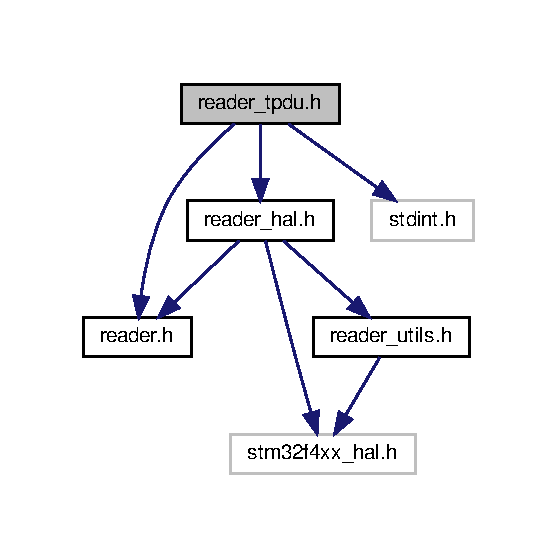
\includegraphics[width=268pt]{reader__tpdu_8h__incl}
\end{center}
\end{figure}
\subsection*{Data Structures}
\begin{DoxyCompactItemize}
\item 
struct \hyperlink{struct_r_e_a_d_e_r___t_p_d_u___header}{R\+E\+A\+D\+E\+R\+\_\+\+T\+P\+D\+U\+\_\+\+Header}
\item 
struct \hyperlink{struct_r_e_a_d_e_r___t_p_d_u___data_field}{R\+E\+A\+D\+E\+R\+\_\+\+T\+P\+D\+U\+\_\+\+Data\+Field}
\item 
struct \hyperlink{struct_r_e_a_d_e_r___t_p_d_u___command}{R\+E\+A\+D\+E\+R\+\_\+\+T\+P\+D\+U\+\_\+\+Command}
\end{DoxyCompactItemize}
\subsection*{Macros}
\begin{DoxyCompactItemize}
\item 
\#define \hyperlink{reader__tpdu_8h_ac2b5682646f650db380874cab59e3e00}{R\+E\+A\+D\+E\+R\+\_\+\+T\+P\+D\+U\+\_\+\+M\+A\+X\+\_\+\+D\+A\+TA}~0x\+FF
\item 
\#define \hyperlink{reader__tpdu_8h_a47b97582f0bd15f961ad03430eca4bcd}{R\+E\+A\+D\+E\+R\+\_\+\+T\+P\+D\+U\+\_\+\+H\+E\+A\+D\+E\+R\+\_\+\+S\+I\+ZE}~5
\item 
\#define \hyperlink{reader__tpdu_8h_a5909fba5d695152971bf0e9a6218efe3}{R\+E\+A\+D\+E\+R\+\_\+\+T\+P\+D\+U\+\_\+\+D\+U\+M\+M\+Y\+\_\+\+F\+A\+L\+S\+E\+\_\+\+I\+NS}~0x61
\item 
\#define \hyperlink{reader__tpdu_8h_a6950d29e0dbd58b7e633c83d6aa546c8}{R\+E\+A\+D\+E\+R\+\_\+\+T\+P\+D\+U\+\_\+\+A\+C\+K\+\_\+\+N\+O\+R\+M\+AL}~0x01
\item 
\#define \hyperlink{reader__tpdu_8h_ad4795a5ccfcdb2baa27757ef091933cc}{R\+E\+A\+D\+E\+R\+\_\+\+T\+P\+D\+U\+\_\+\+A\+C\+K\+\_\+\+X\+O\+R\+ED}~0x02
\end{DoxyCompactItemize}
\subsection*{Typedefs}
\begin{DoxyCompactItemize}
\item 
typedef struct \hyperlink{struct_r_e_a_d_e_r___t_p_d_u___header}{R\+E\+A\+D\+E\+R\+\_\+\+T\+P\+D\+U\+\_\+\+Header} \hyperlink{reader__tpdu_8h_a585471d9405db74c43fe5413336c3e0a}{R\+E\+A\+D\+E\+R\+\_\+\+T\+P\+D\+U\+\_\+\+Header}
\item 
typedef struct \hyperlink{struct_r_e_a_d_e_r___t_p_d_u___data_field}{R\+E\+A\+D\+E\+R\+\_\+\+T\+P\+D\+U\+\_\+\+Data\+Field} \hyperlink{reader__tpdu_8h_aec0605d2ff4be05c4cab7f40d4f3d194}{R\+E\+A\+D\+E\+R\+\_\+\+T\+P\+D\+U\+\_\+\+Data\+Field}
\item 
typedef struct \hyperlink{struct_r_e_a_d_e_r___t_p_d_u___command}{R\+E\+A\+D\+E\+R\+\_\+\+T\+P\+D\+U\+\_\+\+Command} \hyperlink{reader__tpdu_8h_ab55621c3760076dc379540272fa934f3}{R\+E\+A\+D\+E\+R\+\_\+\+T\+P\+D\+U\+\_\+\+Command}
\end{DoxyCompactItemize}
\subsection*{Functions}
\begin{DoxyCompactItemize}
\item 
\hyperlink{reader_8h_a2ce152a8d1e28c2847301451aa5bbc20}{R\+E\+A\+D\+E\+R\+\_\+\+Status} \hyperlink{reader__tpdu_8h_aba8c668a12087e556b0b23d978dde2bb}{R\+E\+A\+D\+E\+R\+\_\+\+T\+P\+D\+U\+\_\+\+Send} (\hyperlink{struct_r_e_a_d_e_r___t_p_d_u___command}{R\+E\+A\+D\+E\+R\+\_\+\+T\+P\+D\+U\+\_\+\+Command} $\ast$tpdu, uint32\+\_\+t timeout)
\item 
\hyperlink{reader_8h_a2ce152a8d1e28c2847301451aa5bbc20}{R\+E\+A\+D\+E\+R\+\_\+\+Status} \hyperlink{reader__tpdu_8h_a097112f09e599488887080e2364da300}{R\+E\+A\+D\+E\+R\+\_\+\+T\+P\+D\+U\+\_\+\+Send\+Header} (\hyperlink{struct_r_e_a_d_e_r___t_p_d_u___command}{R\+E\+A\+D\+E\+R\+\_\+\+T\+P\+D\+U\+\_\+\+Command} $\ast$tpdu, uint32\+\_\+t timeout)
\item 
\hyperlink{reader_8h_a2ce152a8d1e28c2847301451aa5bbc20}{R\+E\+A\+D\+E\+R\+\_\+\+Status} \hyperlink{reader__tpdu_8h_a354524268ee7d089e59c765da89ab260}{R\+E\+A\+D\+E\+R\+\_\+\+T\+P\+D\+U\+\_\+\+Send\+Data\+Oneshot} (\hyperlink{struct_r_e_a_d_e_r___t_p_d_u___command}{R\+E\+A\+D\+E\+R\+\_\+\+T\+P\+D\+U\+\_\+\+Command} $\ast$tpdu, uint32\+\_\+t timeout)
\item 
\hyperlink{reader_8h_a2ce152a8d1e28c2847301451aa5bbc20}{R\+E\+A\+D\+E\+R\+\_\+\+Status} \hyperlink{reader__tpdu_8h_a36f166b57d67bca78e76bb190c527e48}{R\+E\+A\+D\+E\+R\+\_\+\+T\+P\+D\+U\+\_\+\+Send\+Data\+Sliced} (\hyperlink{struct_r_e_a_d_e_r___t_p_d_u___command}{R\+E\+A\+D\+E\+R\+\_\+\+T\+P\+D\+U\+\_\+\+Command} $\ast$tpdu, uint32\+\_\+t timeout)
\item 
\hyperlink{reader_8h_a2ce152a8d1e28c2847301451aa5bbc20}{R\+E\+A\+D\+E\+R\+\_\+\+Status} \hyperlink{reader__tpdu_8h_a2727185d62c7a553ec67ba2695e617a2}{R\+E\+A\+D\+E\+R\+\_\+\+T\+P\+D\+U\+\_\+\+Rcv\+SW} (uint16\+\_\+t $\ast$SW, uint32\+\_\+t timeout)
\item 
\hyperlink{reader_8h_a2ce152a8d1e28c2847301451aa5bbc20}{R\+E\+A\+D\+E\+R\+\_\+\+Status} \hyperlink{reader__tpdu_8h_abbd7e7549bf0c4f15b8c32f7c2a31514}{R\+E\+A\+D\+E\+R\+\_\+\+T\+P\+D\+U\+\_\+\+Wait\+Procedure\+Byte} (uint8\+\_\+t $\ast$procedure\+Byte, uint8\+\_\+t I\+NS, uint32\+\_\+t timeout)
\item 
\hyperlink{reader_8h_a2ce152a8d1e28c2847301451aa5bbc20}{R\+E\+A\+D\+E\+R\+\_\+\+Status} \hyperlink{reader__tpdu_8h_a0b5ad0c94119bef944de7c913c246564}{R\+E\+A\+D\+E\+R\+\_\+\+T\+P\+D\+U\+\_\+\+Wait\+A\+CK} (uint8\+\_\+t I\+NS, uint8\+\_\+t $\ast$A\+C\+K\+Type, uint32\+\_\+t timeout)
\item 
\hyperlink{reader_8h_a2ce152a8d1e28c2847301451aa5bbc20}{R\+E\+A\+D\+E\+R\+\_\+\+Status} \hyperlink{reader__tpdu_8h_a2b581459b9f801ed5e8ca38b166a9820}{R\+E\+A\+D\+E\+R\+\_\+\+T\+P\+D\+U\+\_\+\+Is\+A\+CK} (uint8\+\_\+t byte, uint8\+\_\+t I\+NS)
\item 
\hyperlink{reader_8h_a2ce152a8d1e28c2847301451aa5bbc20}{R\+E\+A\+D\+E\+R\+\_\+\+Status} \hyperlink{reader__tpdu_8h_a3af5e3dc9385453963353167f5a89544}{R\+E\+A\+D\+E\+R\+\_\+\+T\+P\+D\+U\+\_\+\+Is\+Xored\+A\+CK} (uint8\+\_\+t byte, uint8\+\_\+t I\+NS)
\item 
\hyperlink{reader_8h_a2ce152a8d1e28c2847301451aa5bbc20}{R\+E\+A\+D\+E\+R\+\_\+\+Status} \hyperlink{reader__tpdu_8h_acd7714d588af99574aa115dcc9f5d552}{R\+E\+A\+D\+E\+R\+\_\+\+T\+P\+D\+U\+\_\+\+Is\+Null\+Byte} (uint8\+\_\+t byte)
\item 
\hyperlink{reader_8h_a2ce152a8d1e28c2847301451aa5bbc20}{R\+E\+A\+D\+E\+R\+\_\+\+Status} \hyperlink{reader__tpdu_8h_a391b28550859ac80e87b37d90a6cdb02}{R\+E\+A\+D\+E\+R\+\_\+\+T\+P\+D\+U\+\_\+\+Is\+S\+W1} (uint8\+\_\+t byte)
\item 
\hyperlink{reader_8h_a2ce152a8d1e28c2847301451aa5bbc20}{R\+E\+A\+D\+E\+R\+\_\+\+Status} \hyperlink{reader__tpdu_8h_ab85fe276a9c74cd80f05f8dd6f5af1c5}{R\+E\+A\+D\+E\+R\+\_\+\+T\+P\+D\+U\+\_\+\+Is\+Procedure\+Byte} (uint8\+\_\+t byte, uint8\+\_\+t I\+NS)
\item 
\hyperlink{reader_8h_a2ce152a8d1e28c2847301451aa5bbc20}{R\+E\+A\+D\+E\+R\+\_\+\+Status} \hyperlink{reader__tpdu_8h_a4eba8f7c5e42649efd80728290cfd0f5}{R\+E\+A\+D\+E\+R\+\_\+\+T\+P\+D\+U\+\_\+\+Forge} (\hyperlink{struct_r_e_a_d_e_r___t_p_d_u___command}{R\+E\+A\+D\+E\+R\+\_\+\+T\+P\+D\+U\+\_\+\+Command} $\ast$tpdu, uint8\+\_\+t C\+LA, uint8\+\_\+t I\+NS, uint8\+\_\+t P1, uint8\+\_\+t P2, uint8\+\_\+t P3, uint8\+\_\+t $\ast$data\+Buff, uint8\+\_\+t data\+Size)
\end{DoxyCompactItemize}


\subsection{Macro Definition Documentation}
\mbox{\Hypertarget{reader__tpdu_8h_a6950d29e0dbd58b7e633c83d6aa546c8}\label{reader__tpdu_8h_a6950d29e0dbd58b7e633c83d6aa546c8}} 
\index{reader\+\_\+tpdu.\+h@{reader\+\_\+tpdu.\+h}!R\+E\+A\+D\+E\+R\+\_\+\+T\+P\+D\+U\+\_\+\+A\+C\+K\+\_\+\+N\+O\+R\+M\+AL@{R\+E\+A\+D\+E\+R\+\_\+\+T\+P\+D\+U\+\_\+\+A\+C\+K\+\_\+\+N\+O\+R\+M\+AL}}
\index{R\+E\+A\+D\+E\+R\+\_\+\+T\+P\+D\+U\+\_\+\+A\+C\+K\+\_\+\+N\+O\+R\+M\+AL@{R\+E\+A\+D\+E\+R\+\_\+\+T\+P\+D\+U\+\_\+\+A\+C\+K\+\_\+\+N\+O\+R\+M\+AL}!reader\+\_\+tpdu.\+h@{reader\+\_\+tpdu.\+h}}
\subsubsection{\texorpdfstring{R\+E\+A\+D\+E\+R\+\_\+\+T\+P\+D\+U\+\_\+\+A\+C\+K\+\_\+\+N\+O\+R\+M\+AL}{READER\_TPDU\_ACK\_NORMAL}}
{\footnotesize\ttfamily \#define R\+E\+A\+D\+E\+R\+\_\+\+T\+P\+D\+U\+\_\+\+A\+C\+K\+\_\+\+N\+O\+R\+M\+AL~0x01}

\mbox{\Hypertarget{reader__tpdu_8h_ad4795a5ccfcdb2baa27757ef091933cc}\label{reader__tpdu_8h_ad4795a5ccfcdb2baa27757ef091933cc}} 
\index{reader\+\_\+tpdu.\+h@{reader\+\_\+tpdu.\+h}!R\+E\+A\+D\+E\+R\+\_\+\+T\+P\+D\+U\+\_\+\+A\+C\+K\+\_\+\+X\+O\+R\+ED@{R\+E\+A\+D\+E\+R\+\_\+\+T\+P\+D\+U\+\_\+\+A\+C\+K\+\_\+\+X\+O\+R\+ED}}
\index{R\+E\+A\+D\+E\+R\+\_\+\+T\+P\+D\+U\+\_\+\+A\+C\+K\+\_\+\+X\+O\+R\+ED@{R\+E\+A\+D\+E\+R\+\_\+\+T\+P\+D\+U\+\_\+\+A\+C\+K\+\_\+\+X\+O\+R\+ED}!reader\+\_\+tpdu.\+h@{reader\+\_\+tpdu.\+h}}
\subsubsection{\texorpdfstring{R\+E\+A\+D\+E\+R\+\_\+\+T\+P\+D\+U\+\_\+\+A\+C\+K\+\_\+\+X\+O\+R\+ED}{READER\_TPDU\_ACK\_XORED}}
{\footnotesize\ttfamily \#define R\+E\+A\+D\+E\+R\+\_\+\+T\+P\+D\+U\+\_\+\+A\+C\+K\+\_\+\+X\+O\+R\+ED~0x02}

\mbox{\Hypertarget{reader__tpdu_8h_a5909fba5d695152971bf0e9a6218efe3}\label{reader__tpdu_8h_a5909fba5d695152971bf0e9a6218efe3}} 
\index{reader\+\_\+tpdu.\+h@{reader\+\_\+tpdu.\+h}!R\+E\+A\+D\+E\+R\+\_\+\+T\+P\+D\+U\+\_\+\+D\+U\+M\+M\+Y\+\_\+\+F\+A\+L\+S\+E\+\_\+\+I\+NS@{R\+E\+A\+D\+E\+R\+\_\+\+T\+P\+D\+U\+\_\+\+D\+U\+M\+M\+Y\+\_\+\+F\+A\+L\+S\+E\+\_\+\+I\+NS}}
\index{R\+E\+A\+D\+E\+R\+\_\+\+T\+P\+D\+U\+\_\+\+D\+U\+M\+M\+Y\+\_\+\+F\+A\+L\+S\+E\+\_\+\+I\+NS@{R\+E\+A\+D\+E\+R\+\_\+\+T\+P\+D\+U\+\_\+\+D\+U\+M\+M\+Y\+\_\+\+F\+A\+L\+S\+E\+\_\+\+I\+NS}!reader\+\_\+tpdu.\+h@{reader\+\_\+tpdu.\+h}}
\subsubsection{\texorpdfstring{R\+E\+A\+D\+E\+R\+\_\+\+T\+P\+D\+U\+\_\+\+D\+U\+M\+M\+Y\+\_\+\+F\+A\+L\+S\+E\+\_\+\+I\+NS}{READER\_TPDU\_DUMMY\_FALSE\_INS}}
{\footnotesize\ttfamily \#define R\+E\+A\+D\+E\+R\+\_\+\+T\+P\+D\+U\+\_\+\+D\+U\+M\+M\+Y\+\_\+\+F\+A\+L\+S\+E\+\_\+\+I\+NS~0x61}

\mbox{\Hypertarget{reader__tpdu_8h_a47b97582f0bd15f961ad03430eca4bcd}\label{reader__tpdu_8h_a47b97582f0bd15f961ad03430eca4bcd}} 
\index{reader\+\_\+tpdu.\+h@{reader\+\_\+tpdu.\+h}!R\+E\+A\+D\+E\+R\+\_\+\+T\+P\+D\+U\+\_\+\+H\+E\+A\+D\+E\+R\+\_\+\+S\+I\+ZE@{R\+E\+A\+D\+E\+R\+\_\+\+T\+P\+D\+U\+\_\+\+H\+E\+A\+D\+E\+R\+\_\+\+S\+I\+ZE}}
\index{R\+E\+A\+D\+E\+R\+\_\+\+T\+P\+D\+U\+\_\+\+H\+E\+A\+D\+E\+R\+\_\+\+S\+I\+ZE@{R\+E\+A\+D\+E\+R\+\_\+\+T\+P\+D\+U\+\_\+\+H\+E\+A\+D\+E\+R\+\_\+\+S\+I\+ZE}!reader\+\_\+tpdu.\+h@{reader\+\_\+tpdu.\+h}}
\subsubsection{\texorpdfstring{R\+E\+A\+D\+E\+R\+\_\+\+T\+P\+D\+U\+\_\+\+H\+E\+A\+D\+E\+R\+\_\+\+S\+I\+ZE}{READER\_TPDU\_HEADER\_SIZE}}
{\footnotesize\ttfamily \#define R\+E\+A\+D\+E\+R\+\_\+\+T\+P\+D\+U\+\_\+\+H\+E\+A\+D\+E\+R\+\_\+\+S\+I\+ZE~5}

\mbox{\Hypertarget{reader__tpdu_8h_ac2b5682646f650db380874cab59e3e00}\label{reader__tpdu_8h_ac2b5682646f650db380874cab59e3e00}} 
\index{reader\+\_\+tpdu.\+h@{reader\+\_\+tpdu.\+h}!R\+E\+A\+D\+E\+R\+\_\+\+T\+P\+D\+U\+\_\+\+M\+A\+X\+\_\+\+D\+A\+TA@{R\+E\+A\+D\+E\+R\+\_\+\+T\+P\+D\+U\+\_\+\+M\+A\+X\+\_\+\+D\+A\+TA}}
\index{R\+E\+A\+D\+E\+R\+\_\+\+T\+P\+D\+U\+\_\+\+M\+A\+X\+\_\+\+D\+A\+TA@{R\+E\+A\+D\+E\+R\+\_\+\+T\+P\+D\+U\+\_\+\+M\+A\+X\+\_\+\+D\+A\+TA}!reader\+\_\+tpdu.\+h@{reader\+\_\+tpdu.\+h}}
\subsubsection{\texorpdfstring{R\+E\+A\+D\+E\+R\+\_\+\+T\+P\+D\+U\+\_\+\+M\+A\+X\+\_\+\+D\+A\+TA}{READER\_TPDU\_MAX\_DATA}}
{\footnotesize\ttfamily \#define R\+E\+A\+D\+E\+R\+\_\+\+T\+P\+D\+U\+\_\+\+M\+A\+X\+\_\+\+D\+A\+TA~0x\+FF}



\subsection{Typedef Documentation}
\mbox{\Hypertarget{reader__tpdu_8h_ab55621c3760076dc379540272fa934f3}\label{reader__tpdu_8h_ab55621c3760076dc379540272fa934f3}} 
\index{reader\+\_\+tpdu.\+h@{reader\+\_\+tpdu.\+h}!R\+E\+A\+D\+E\+R\+\_\+\+T\+P\+D\+U\+\_\+\+Command@{R\+E\+A\+D\+E\+R\+\_\+\+T\+P\+D\+U\+\_\+\+Command}}
\index{R\+E\+A\+D\+E\+R\+\_\+\+T\+P\+D\+U\+\_\+\+Command@{R\+E\+A\+D\+E\+R\+\_\+\+T\+P\+D\+U\+\_\+\+Command}!reader\+\_\+tpdu.\+h@{reader\+\_\+tpdu.\+h}}
\subsubsection{\texorpdfstring{R\+E\+A\+D\+E\+R\+\_\+\+T\+P\+D\+U\+\_\+\+Command}{READER\_TPDU\_Command}}
{\footnotesize\ttfamily typedef struct \hyperlink{struct_r_e_a_d_e_r___t_p_d_u___command}{R\+E\+A\+D\+E\+R\+\_\+\+T\+P\+D\+U\+\_\+\+Command} \hyperlink{struct_r_e_a_d_e_r___t_p_d_u___command}{R\+E\+A\+D\+E\+R\+\_\+\+T\+P\+D\+U\+\_\+\+Command}}

\mbox{\Hypertarget{reader__tpdu_8h_aec0605d2ff4be05c4cab7f40d4f3d194}\label{reader__tpdu_8h_aec0605d2ff4be05c4cab7f40d4f3d194}} 
\index{reader\+\_\+tpdu.\+h@{reader\+\_\+tpdu.\+h}!R\+E\+A\+D\+E\+R\+\_\+\+T\+P\+D\+U\+\_\+\+Data\+Field@{R\+E\+A\+D\+E\+R\+\_\+\+T\+P\+D\+U\+\_\+\+Data\+Field}}
\index{R\+E\+A\+D\+E\+R\+\_\+\+T\+P\+D\+U\+\_\+\+Data\+Field@{R\+E\+A\+D\+E\+R\+\_\+\+T\+P\+D\+U\+\_\+\+Data\+Field}!reader\+\_\+tpdu.\+h@{reader\+\_\+tpdu.\+h}}
\subsubsection{\texorpdfstring{R\+E\+A\+D\+E\+R\+\_\+\+T\+P\+D\+U\+\_\+\+Data\+Field}{READER\_TPDU\_DataField}}
{\footnotesize\ttfamily typedef struct \hyperlink{struct_r_e_a_d_e_r___t_p_d_u___data_field}{R\+E\+A\+D\+E\+R\+\_\+\+T\+P\+D\+U\+\_\+\+Data\+Field} \hyperlink{struct_r_e_a_d_e_r___t_p_d_u___data_field}{R\+E\+A\+D\+E\+R\+\_\+\+T\+P\+D\+U\+\_\+\+Data\+Field}}

\mbox{\Hypertarget{reader__tpdu_8h_a585471d9405db74c43fe5413336c3e0a}\label{reader__tpdu_8h_a585471d9405db74c43fe5413336c3e0a}} 
\index{reader\+\_\+tpdu.\+h@{reader\+\_\+tpdu.\+h}!R\+E\+A\+D\+E\+R\+\_\+\+T\+P\+D\+U\+\_\+\+Header@{R\+E\+A\+D\+E\+R\+\_\+\+T\+P\+D\+U\+\_\+\+Header}}
\index{R\+E\+A\+D\+E\+R\+\_\+\+T\+P\+D\+U\+\_\+\+Header@{R\+E\+A\+D\+E\+R\+\_\+\+T\+P\+D\+U\+\_\+\+Header}!reader\+\_\+tpdu.\+h@{reader\+\_\+tpdu.\+h}}
\subsubsection{\texorpdfstring{R\+E\+A\+D\+E\+R\+\_\+\+T\+P\+D\+U\+\_\+\+Header}{READER\_TPDU\_Header}}
{\footnotesize\ttfamily typedef struct \hyperlink{struct_r_e_a_d_e_r___t_p_d_u___header}{R\+E\+A\+D\+E\+R\+\_\+\+T\+P\+D\+U\+\_\+\+Header} \hyperlink{struct_r_e_a_d_e_r___t_p_d_u___header}{R\+E\+A\+D\+E\+R\+\_\+\+T\+P\+D\+U\+\_\+\+Header}}



\subsection{Function Documentation}
\mbox{\Hypertarget{reader__tpdu_8h_a4eba8f7c5e42649efd80728290cfd0f5}\label{reader__tpdu_8h_a4eba8f7c5e42649efd80728290cfd0f5}} 
\index{reader\+\_\+tpdu.\+h@{reader\+\_\+tpdu.\+h}!R\+E\+A\+D\+E\+R\+\_\+\+T\+P\+D\+U\+\_\+\+Forge@{R\+E\+A\+D\+E\+R\+\_\+\+T\+P\+D\+U\+\_\+\+Forge}}
\index{R\+E\+A\+D\+E\+R\+\_\+\+T\+P\+D\+U\+\_\+\+Forge@{R\+E\+A\+D\+E\+R\+\_\+\+T\+P\+D\+U\+\_\+\+Forge}!reader\+\_\+tpdu.\+h@{reader\+\_\+tpdu.\+h}}
\subsubsection{\texorpdfstring{R\+E\+A\+D\+E\+R\+\_\+\+T\+P\+D\+U\+\_\+\+Forge()}{READER\_TPDU\_Forge()}}
{\footnotesize\ttfamily \hyperlink{reader_8h_a2ce152a8d1e28c2847301451aa5bbc20}{R\+E\+A\+D\+E\+R\+\_\+\+Status} R\+E\+A\+D\+E\+R\+\_\+\+T\+P\+D\+U\+\_\+\+Forge (\begin{DoxyParamCaption}\item[{\hyperlink{struct_r_e_a_d_e_r___t_p_d_u___command}{R\+E\+A\+D\+E\+R\+\_\+\+T\+P\+D\+U\+\_\+\+Command} $\ast$}]{tpdu,  }\item[{uint8\+\_\+t}]{C\+LA,  }\item[{uint8\+\_\+t}]{I\+NS,  }\item[{uint8\+\_\+t}]{P1,  }\item[{uint8\+\_\+t}]{P2,  }\item[{uint8\+\_\+t}]{P3,  }\item[{uint8\+\_\+t $\ast$}]{data\+Buff,  }\item[{uint8\+\_\+t}]{data\+Size }\end{DoxyParamCaption})}

\mbox{\Hypertarget{reader__tpdu_8h_a2b581459b9f801ed5e8ca38b166a9820}\label{reader__tpdu_8h_a2b581459b9f801ed5e8ca38b166a9820}} 
\index{reader\+\_\+tpdu.\+h@{reader\+\_\+tpdu.\+h}!R\+E\+A\+D\+E\+R\+\_\+\+T\+P\+D\+U\+\_\+\+Is\+A\+CK@{R\+E\+A\+D\+E\+R\+\_\+\+T\+P\+D\+U\+\_\+\+Is\+A\+CK}}
\index{R\+E\+A\+D\+E\+R\+\_\+\+T\+P\+D\+U\+\_\+\+Is\+A\+CK@{R\+E\+A\+D\+E\+R\+\_\+\+T\+P\+D\+U\+\_\+\+Is\+A\+CK}!reader\+\_\+tpdu.\+h@{reader\+\_\+tpdu.\+h}}
\subsubsection{\texorpdfstring{R\+E\+A\+D\+E\+R\+\_\+\+T\+P\+D\+U\+\_\+\+Is\+A\+C\+K()}{READER\_TPDU\_IsACK()}}
{\footnotesize\ttfamily \hyperlink{reader_8h_a2ce152a8d1e28c2847301451aa5bbc20}{R\+E\+A\+D\+E\+R\+\_\+\+Status} R\+E\+A\+D\+E\+R\+\_\+\+T\+P\+D\+U\+\_\+\+Is\+A\+CK (\begin{DoxyParamCaption}\item[{uint8\+\_\+t}]{byte,  }\item[{uint8\+\_\+t}]{I\+NS }\end{DoxyParamCaption})}

\mbox{\Hypertarget{reader__tpdu_8h_acd7714d588af99574aa115dcc9f5d552}\label{reader__tpdu_8h_acd7714d588af99574aa115dcc9f5d552}} 
\index{reader\+\_\+tpdu.\+h@{reader\+\_\+tpdu.\+h}!R\+E\+A\+D\+E\+R\+\_\+\+T\+P\+D\+U\+\_\+\+Is\+Null\+Byte@{R\+E\+A\+D\+E\+R\+\_\+\+T\+P\+D\+U\+\_\+\+Is\+Null\+Byte}}
\index{R\+E\+A\+D\+E\+R\+\_\+\+T\+P\+D\+U\+\_\+\+Is\+Null\+Byte@{R\+E\+A\+D\+E\+R\+\_\+\+T\+P\+D\+U\+\_\+\+Is\+Null\+Byte}!reader\+\_\+tpdu.\+h@{reader\+\_\+tpdu.\+h}}
\subsubsection{\texorpdfstring{R\+E\+A\+D\+E\+R\+\_\+\+T\+P\+D\+U\+\_\+\+Is\+Null\+Byte()}{READER\_TPDU\_IsNullByte()}}
{\footnotesize\ttfamily \hyperlink{reader_8h_a2ce152a8d1e28c2847301451aa5bbc20}{R\+E\+A\+D\+E\+R\+\_\+\+Status} R\+E\+A\+D\+E\+R\+\_\+\+T\+P\+D\+U\+\_\+\+Is\+Null\+Byte (\begin{DoxyParamCaption}\item[{uint8\+\_\+t}]{byte }\end{DoxyParamCaption})}

\mbox{\Hypertarget{reader__tpdu_8h_ab85fe276a9c74cd80f05f8dd6f5af1c5}\label{reader__tpdu_8h_ab85fe276a9c74cd80f05f8dd6f5af1c5}} 
\index{reader\+\_\+tpdu.\+h@{reader\+\_\+tpdu.\+h}!R\+E\+A\+D\+E\+R\+\_\+\+T\+P\+D\+U\+\_\+\+Is\+Procedure\+Byte@{R\+E\+A\+D\+E\+R\+\_\+\+T\+P\+D\+U\+\_\+\+Is\+Procedure\+Byte}}
\index{R\+E\+A\+D\+E\+R\+\_\+\+T\+P\+D\+U\+\_\+\+Is\+Procedure\+Byte@{R\+E\+A\+D\+E\+R\+\_\+\+T\+P\+D\+U\+\_\+\+Is\+Procedure\+Byte}!reader\+\_\+tpdu.\+h@{reader\+\_\+tpdu.\+h}}
\subsubsection{\texorpdfstring{R\+E\+A\+D\+E\+R\+\_\+\+T\+P\+D\+U\+\_\+\+Is\+Procedure\+Byte()}{READER\_TPDU\_IsProcedureByte()}}
{\footnotesize\ttfamily \hyperlink{reader_8h_a2ce152a8d1e28c2847301451aa5bbc20}{R\+E\+A\+D\+E\+R\+\_\+\+Status} R\+E\+A\+D\+E\+R\+\_\+\+T\+P\+D\+U\+\_\+\+Is\+Procedure\+Byte (\begin{DoxyParamCaption}\item[{uint8\+\_\+t}]{byte,  }\item[{uint8\+\_\+t}]{I\+NS }\end{DoxyParamCaption})}

\mbox{\Hypertarget{reader__tpdu_8h_a391b28550859ac80e87b37d90a6cdb02}\label{reader__tpdu_8h_a391b28550859ac80e87b37d90a6cdb02}} 
\index{reader\+\_\+tpdu.\+h@{reader\+\_\+tpdu.\+h}!R\+E\+A\+D\+E\+R\+\_\+\+T\+P\+D\+U\+\_\+\+Is\+S\+W1@{R\+E\+A\+D\+E\+R\+\_\+\+T\+P\+D\+U\+\_\+\+Is\+S\+W1}}
\index{R\+E\+A\+D\+E\+R\+\_\+\+T\+P\+D\+U\+\_\+\+Is\+S\+W1@{R\+E\+A\+D\+E\+R\+\_\+\+T\+P\+D\+U\+\_\+\+Is\+S\+W1}!reader\+\_\+tpdu.\+h@{reader\+\_\+tpdu.\+h}}
\subsubsection{\texorpdfstring{R\+E\+A\+D\+E\+R\+\_\+\+T\+P\+D\+U\+\_\+\+Is\+S\+W1()}{READER\_TPDU\_IsSW1()}}
{\footnotesize\ttfamily \hyperlink{reader_8h_a2ce152a8d1e28c2847301451aa5bbc20}{R\+E\+A\+D\+E\+R\+\_\+\+Status} R\+E\+A\+D\+E\+R\+\_\+\+T\+P\+D\+U\+\_\+\+Is\+S\+W1 (\begin{DoxyParamCaption}\item[{uint8\+\_\+t}]{byte }\end{DoxyParamCaption})}

\mbox{\Hypertarget{reader__tpdu_8h_a3af5e3dc9385453963353167f5a89544}\label{reader__tpdu_8h_a3af5e3dc9385453963353167f5a89544}} 
\index{reader\+\_\+tpdu.\+h@{reader\+\_\+tpdu.\+h}!R\+E\+A\+D\+E\+R\+\_\+\+T\+P\+D\+U\+\_\+\+Is\+Xored\+A\+CK@{R\+E\+A\+D\+E\+R\+\_\+\+T\+P\+D\+U\+\_\+\+Is\+Xored\+A\+CK}}
\index{R\+E\+A\+D\+E\+R\+\_\+\+T\+P\+D\+U\+\_\+\+Is\+Xored\+A\+CK@{R\+E\+A\+D\+E\+R\+\_\+\+T\+P\+D\+U\+\_\+\+Is\+Xored\+A\+CK}!reader\+\_\+tpdu.\+h@{reader\+\_\+tpdu.\+h}}
\subsubsection{\texorpdfstring{R\+E\+A\+D\+E\+R\+\_\+\+T\+P\+D\+U\+\_\+\+Is\+Xored\+A\+C\+K()}{READER\_TPDU\_IsXoredACK()}}
{\footnotesize\ttfamily \hyperlink{reader_8h_a2ce152a8d1e28c2847301451aa5bbc20}{R\+E\+A\+D\+E\+R\+\_\+\+Status} R\+E\+A\+D\+E\+R\+\_\+\+T\+P\+D\+U\+\_\+\+Is\+Xored\+A\+CK (\begin{DoxyParamCaption}\item[{uint8\+\_\+t}]{byte,  }\item[{uint8\+\_\+t}]{I\+NS }\end{DoxyParamCaption})}

\mbox{\Hypertarget{reader__tpdu_8h_a2727185d62c7a553ec67ba2695e617a2}\label{reader__tpdu_8h_a2727185d62c7a553ec67ba2695e617a2}} 
\index{reader\+\_\+tpdu.\+h@{reader\+\_\+tpdu.\+h}!R\+E\+A\+D\+E\+R\+\_\+\+T\+P\+D\+U\+\_\+\+Rcv\+SW@{R\+E\+A\+D\+E\+R\+\_\+\+T\+P\+D\+U\+\_\+\+Rcv\+SW}}
\index{R\+E\+A\+D\+E\+R\+\_\+\+T\+P\+D\+U\+\_\+\+Rcv\+SW@{R\+E\+A\+D\+E\+R\+\_\+\+T\+P\+D\+U\+\_\+\+Rcv\+SW}!reader\+\_\+tpdu.\+h@{reader\+\_\+tpdu.\+h}}
\subsubsection{\texorpdfstring{R\+E\+A\+D\+E\+R\+\_\+\+T\+P\+D\+U\+\_\+\+Rcv\+S\+W()}{READER\_TPDU\_RcvSW()}}
{\footnotesize\ttfamily \hyperlink{reader_8h_a2ce152a8d1e28c2847301451aa5bbc20}{R\+E\+A\+D\+E\+R\+\_\+\+Status} R\+E\+A\+D\+E\+R\+\_\+\+T\+P\+D\+U\+\_\+\+Rcv\+SW (\begin{DoxyParamCaption}\item[{uint16\+\_\+t $\ast$}]{SW,  }\item[{uint32\+\_\+t}]{timeout }\end{DoxyParamCaption})}

\mbox{\Hypertarget{reader__tpdu_8h_aba8c668a12087e556b0b23d978dde2bb}\label{reader__tpdu_8h_aba8c668a12087e556b0b23d978dde2bb}} 
\index{reader\+\_\+tpdu.\+h@{reader\+\_\+tpdu.\+h}!R\+E\+A\+D\+E\+R\+\_\+\+T\+P\+D\+U\+\_\+\+Send@{R\+E\+A\+D\+E\+R\+\_\+\+T\+P\+D\+U\+\_\+\+Send}}
\index{R\+E\+A\+D\+E\+R\+\_\+\+T\+P\+D\+U\+\_\+\+Send@{R\+E\+A\+D\+E\+R\+\_\+\+T\+P\+D\+U\+\_\+\+Send}!reader\+\_\+tpdu.\+h@{reader\+\_\+tpdu.\+h}}
\subsubsection{\texorpdfstring{R\+E\+A\+D\+E\+R\+\_\+\+T\+P\+D\+U\+\_\+\+Send()}{READER\_TPDU\_Send()}}
{\footnotesize\ttfamily \hyperlink{reader_8h_a2ce152a8d1e28c2847301451aa5bbc20}{R\+E\+A\+D\+E\+R\+\_\+\+Status} R\+E\+A\+D\+E\+R\+\_\+\+T\+P\+D\+U\+\_\+\+Send (\begin{DoxyParamCaption}\item[{\hyperlink{struct_r_e_a_d_e_r___t_p_d_u___command}{R\+E\+A\+D\+E\+R\+\_\+\+T\+P\+D\+U\+\_\+\+Command} $\ast$}]{tpdu,  }\item[{uint32\+\_\+t}]{timeout }\end{DoxyParamCaption})}

\mbox{\Hypertarget{reader__tpdu_8h_a354524268ee7d089e59c765da89ab260}\label{reader__tpdu_8h_a354524268ee7d089e59c765da89ab260}} 
\index{reader\+\_\+tpdu.\+h@{reader\+\_\+tpdu.\+h}!R\+E\+A\+D\+E\+R\+\_\+\+T\+P\+D\+U\+\_\+\+Send\+Data\+Oneshot@{R\+E\+A\+D\+E\+R\+\_\+\+T\+P\+D\+U\+\_\+\+Send\+Data\+Oneshot}}
\index{R\+E\+A\+D\+E\+R\+\_\+\+T\+P\+D\+U\+\_\+\+Send\+Data\+Oneshot@{R\+E\+A\+D\+E\+R\+\_\+\+T\+P\+D\+U\+\_\+\+Send\+Data\+Oneshot}!reader\+\_\+tpdu.\+h@{reader\+\_\+tpdu.\+h}}
\subsubsection{\texorpdfstring{R\+E\+A\+D\+E\+R\+\_\+\+T\+P\+D\+U\+\_\+\+Send\+Data\+Oneshot()}{READER\_TPDU\_SendDataOneshot()}}
{\footnotesize\ttfamily \hyperlink{reader_8h_a2ce152a8d1e28c2847301451aa5bbc20}{R\+E\+A\+D\+E\+R\+\_\+\+Status} R\+E\+A\+D\+E\+R\+\_\+\+T\+P\+D\+U\+\_\+\+Send\+Data\+Oneshot (\begin{DoxyParamCaption}\item[{\hyperlink{struct_r_e_a_d_e_r___t_p_d_u___command}{R\+E\+A\+D\+E\+R\+\_\+\+T\+P\+D\+U\+\_\+\+Command} $\ast$}]{tpdu,  }\item[{uint32\+\_\+t}]{timeout }\end{DoxyParamCaption})}

\mbox{\Hypertarget{reader__tpdu_8h_a36f166b57d67bca78e76bb190c527e48}\label{reader__tpdu_8h_a36f166b57d67bca78e76bb190c527e48}} 
\index{reader\+\_\+tpdu.\+h@{reader\+\_\+tpdu.\+h}!R\+E\+A\+D\+E\+R\+\_\+\+T\+P\+D\+U\+\_\+\+Send\+Data\+Sliced@{R\+E\+A\+D\+E\+R\+\_\+\+T\+P\+D\+U\+\_\+\+Send\+Data\+Sliced}}
\index{R\+E\+A\+D\+E\+R\+\_\+\+T\+P\+D\+U\+\_\+\+Send\+Data\+Sliced@{R\+E\+A\+D\+E\+R\+\_\+\+T\+P\+D\+U\+\_\+\+Send\+Data\+Sliced}!reader\+\_\+tpdu.\+h@{reader\+\_\+tpdu.\+h}}
\subsubsection{\texorpdfstring{R\+E\+A\+D\+E\+R\+\_\+\+T\+P\+D\+U\+\_\+\+Send\+Data\+Sliced()}{READER\_TPDU\_SendDataSliced()}}
{\footnotesize\ttfamily \hyperlink{reader_8h_a2ce152a8d1e28c2847301451aa5bbc20}{R\+E\+A\+D\+E\+R\+\_\+\+Status} R\+E\+A\+D\+E\+R\+\_\+\+T\+P\+D\+U\+\_\+\+Send\+Data\+Sliced (\begin{DoxyParamCaption}\item[{\hyperlink{struct_r_e_a_d_e_r___t_p_d_u___command}{R\+E\+A\+D\+E\+R\+\_\+\+T\+P\+D\+U\+\_\+\+Command} $\ast$}]{tpdu,  }\item[{uint32\+\_\+t}]{timeout }\end{DoxyParamCaption})}

\mbox{\Hypertarget{reader__tpdu_8h_a097112f09e599488887080e2364da300}\label{reader__tpdu_8h_a097112f09e599488887080e2364da300}} 
\index{reader\+\_\+tpdu.\+h@{reader\+\_\+tpdu.\+h}!R\+E\+A\+D\+E\+R\+\_\+\+T\+P\+D\+U\+\_\+\+Send\+Header@{R\+E\+A\+D\+E\+R\+\_\+\+T\+P\+D\+U\+\_\+\+Send\+Header}}
\index{R\+E\+A\+D\+E\+R\+\_\+\+T\+P\+D\+U\+\_\+\+Send\+Header@{R\+E\+A\+D\+E\+R\+\_\+\+T\+P\+D\+U\+\_\+\+Send\+Header}!reader\+\_\+tpdu.\+h@{reader\+\_\+tpdu.\+h}}
\subsubsection{\texorpdfstring{R\+E\+A\+D\+E\+R\+\_\+\+T\+P\+D\+U\+\_\+\+Send\+Header()}{READER\_TPDU\_SendHeader()}}
{\footnotesize\ttfamily \hyperlink{reader_8h_a2ce152a8d1e28c2847301451aa5bbc20}{R\+E\+A\+D\+E\+R\+\_\+\+Status} R\+E\+A\+D\+E\+R\+\_\+\+T\+P\+D\+U\+\_\+\+Send\+Header (\begin{DoxyParamCaption}\item[{\hyperlink{struct_r_e_a_d_e_r___t_p_d_u___command}{R\+E\+A\+D\+E\+R\+\_\+\+T\+P\+D\+U\+\_\+\+Command} $\ast$}]{tpdu,  }\item[{uint32\+\_\+t}]{timeout }\end{DoxyParamCaption})}

\mbox{\Hypertarget{reader__tpdu_8h_a0b5ad0c94119bef944de7c913c246564}\label{reader__tpdu_8h_a0b5ad0c94119bef944de7c913c246564}} 
\index{reader\+\_\+tpdu.\+h@{reader\+\_\+tpdu.\+h}!R\+E\+A\+D\+E\+R\+\_\+\+T\+P\+D\+U\+\_\+\+Wait\+A\+CK@{R\+E\+A\+D\+E\+R\+\_\+\+T\+P\+D\+U\+\_\+\+Wait\+A\+CK}}
\index{R\+E\+A\+D\+E\+R\+\_\+\+T\+P\+D\+U\+\_\+\+Wait\+A\+CK@{R\+E\+A\+D\+E\+R\+\_\+\+T\+P\+D\+U\+\_\+\+Wait\+A\+CK}!reader\+\_\+tpdu.\+h@{reader\+\_\+tpdu.\+h}}
\subsubsection{\texorpdfstring{R\+E\+A\+D\+E\+R\+\_\+\+T\+P\+D\+U\+\_\+\+Wait\+A\+C\+K()}{READER\_TPDU\_WaitACK()}}
{\footnotesize\ttfamily \hyperlink{reader_8h_a2ce152a8d1e28c2847301451aa5bbc20}{R\+E\+A\+D\+E\+R\+\_\+\+Status} R\+E\+A\+D\+E\+R\+\_\+\+T\+P\+D\+U\+\_\+\+Wait\+A\+CK (\begin{DoxyParamCaption}\item[{uint8\+\_\+t}]{I\+NS,  }\item[{uint8\+\_\+t $\ast$}]{A\+C\+K\+Type,  }\item[{uint32\+\_\+t}]{timeout }\end{DoxyParamCaption})}

\mbox{\Hypertarget{reader__tpdu_8h_abbd7e7549bf0c4f15b8c32f7c2a31514}\label{reader__tpdu_8h_abbd7e7549bf0c4f15b8c32f7c2a31514}} 
\index{reader\+\_\+tpdu.\+h@{reader\+\_\+tpdu.\+h}!R\+E\+A\+D\+E\+R\+\_\+\+T\+P\+D\+U\+\_\+\+Wait\+Procedure\+Byte@{R\+E\+A\+D\+E\+R\+\_\+\+T\+P\+D\+U\+\_\+\+Wait\+Procedure\+Byte}}
\index{R\+E\+A\+D\+E\+R\+\_\+\+T\+P\+D\+U\+\_\+\+Wait\+Procedure\+Byte@{R\+E\+A\+D\+E\+R\+\_\+\+T\+P\+D\+U\+\_\+\+Wait\+Procedure\+Byte}!reader\+\_\+tpdu.\+h@{reader\+\_\+tpdu.\+h}}
\subsubsection{\texorpdfstring{R\+E\+A\+D\+E\+R\+\_\+\+T\+P\+D\+U\+\_\+\+Wait\+Procedure\+Byte()}{READER\_TPDU\_WaitProcedureByte()}}
{\footnotesize\ttfamily \hyperlink{reader_8h_a2ce152a8d1e28c2847301451aa5bbc20}{R\+E\+A\+D\+E\+R\+\_\+\+Status} R\+E\+A\+D\+E\+R\+\_\+\+T\+P\+D\+U\+\_\+\+Wait\+Procedure\+Byte (\begin{DoxyParamCaption}\item[{uint8\+\_\+t $\ast$}]{procedure\+Byte,  }\item[{uint8\+\_\+t}]{I\+NS,  }\item[{uint32\+\_\+t}]{timeout }\end{DoxyParamCaption})}


\hypertarget{reader__utils_8h}{}\section{reader\+\_\+utils.\+h File Reference}
\label{reader__utils_8h}\index{reader\+\_\+utils.\+h@{reader\+\_\+utils.\+h}}
{\ttfamily \#include \char`\"{}stm32f4xx\+\_\+hal.\+h\char`\"{}}\newline
Include dependency graph for reader\+\_\+utils.\+h\+:
\nopagebreak
\begin{figure}[H]
\begin{center}
\leavevmode
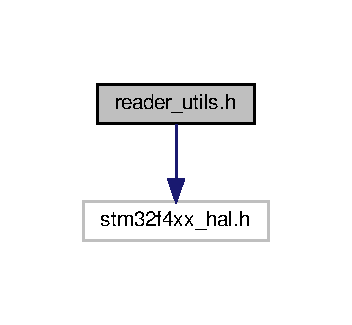
\includegraphics[width=169pt]{reader__utils_8h__incl}
\end{center}
\end{figure}
This graph shows which files directly or indirectly include this file\+:
\nopagebreak
\begin{figure}[H]
\begin{center}
\leavevmode
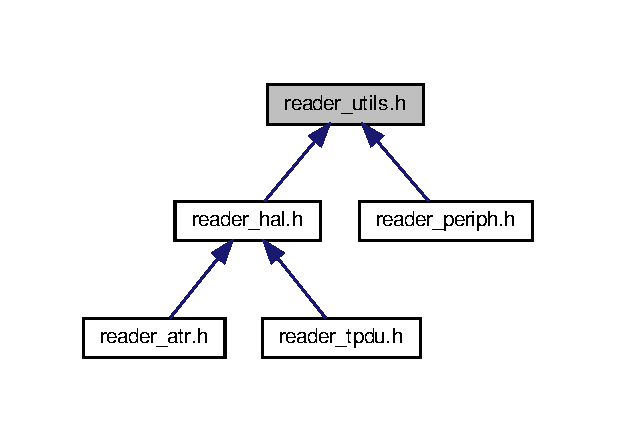
\includegraphics[width=296pt]{reader__utils_8h__dep__incl}
\end{center}
\end{figure}
\subsection*{Functions}
\begin{DoxyCompactItemize}
\item 
uint32\+\_\+t \hyperlink{reader__utils_8h_ad61578239a5eff2d84617c656da0bff1}{R\+E\+A\+D\+E\+R\+\_\+\+U\+T\+I\+L\+S\+\_\+\+Compute\+Baud\+Rate} (uint32\+\_\+t freq, uint32\+\_\+t Fi, uint32\+\_\+t Di)
\item 
uint32\+\_\+t \hyperlink{reader__utils_8h_a7d664462b6e6c4b5487dffe807f8e0f1}{R\+E\+A\+D\+E\+R\+\_\+\+U\+T\+I\+L\+S\+\_\+\+Get\+Card\+Freq} (uint32\+\_\+t S\+Y\+S\+C\+LK, uint32\+\_\+t A\+HB, uint32\+\_\+t A\+P\+B1, uint32\+\_\+t value\+\_\+\+U\+S\+A\+R\+T\+\_\+\+G\+T\+P\+R\+\_\+\+P\+SC)
\item 
uint32\+\_\+t \hyperlink{reader__utils_8h_aae5c805c5880a79fac772f5367bb4905}{R\+E\+A\+D\+E\+R\+\_\+\+U\+T\+I\+L\+S\+\_\+\+Compute\+New\+Baud\+Rate} (uint32\+\_\+t old\+Baud\+Rate, uint32\+\_\+t old\+Freq, uint32\+\_\+t new\+Freq)
\item 
uint32\+\_\+t \hyperlink{reader__utils_8h_a9e1e975ef9f4495b34c9b5d4f917bd5b}{R\+E\+A\+D\+E\+R\+\_\+\+U\+T\+I\+L\+S\+\_\+\+Compute\+Presc\+From\+Freq} (uint32\+\_\+t freq)
\item 
uint32\+\_\+t \hyperlink{reader__utils_8h_a2bcf3bc539b209eb960ee9c40b5ebf6b}{R\+E\+A\+D\+E\+R\+\_\+\+U\+T\+I\+L\+S\+\_\+\+Compute\+Timeout\+Mili\+Sec} (uint32\+\_\+t baud\+Rate, uint32\+\_\+t WT)
\end{DoxyCompactItemize}


\subsection{Function Documentation}
\mbox{\Hypertarget{reader__utils_8h_ad61578239a5eff2d84617c656da0bff1}\label{reader__utils_8h_ad61578239a5eff2d84617c656da0bff1}} 
\index{reader\+\_\+utils.\+h@{reader\+\_\+utils.\+h}!R\+E\+A\+D\+E\+R\+\_\+\+U\+T\+I\+L\+S\+\_\+\+Compute\+Baud\+Rate@{R\+E\+A\+D\+E\+R\+\_\+\+U\+T\+I\+L\+S\+\_\+\+Compute\+Baud\+Rate}}
\index{R\+E\+A\+D\+E\+R\+\_\+\+U\+T\+I\+L\+S\+\_\+\+Compute\+Baud\+Rate@{R\+E\+A\+D\+E\+R\+\_\+\+U\+T\+I\+L\+S\+\_\+\+Compute\+Baud\+Rate}!reader\+\_\+utils.\+h@{reader\+\_\+utils.\+h}}
\subsubsection{\texorpdfstring{R\+E\+A\+D\+E\+R\+\_\+\+U\+T\+I\+L\+S\+\_\+\+Compute\+Baud\+Rate()}{READER\_UTILS\_ComputeBaudRate()}}
{\footnotesize\ttfamily uint32\+\_\+t R\+E\+A\+D\+E\+R\+\_\+\+U\+T\+I\+L\+S\+\_\+\+Compute\+Baud\+Rate (\begin{DoxyParamCaption}\item[{uint32\+\_\+t}]{freq,  }\item[{uint32\+\_\+t}]{Fi,  }\item[{uint32\+\_\+t}]{Di }\end{DoxyParamCaption})}

\mbox{\Hypertarget{reader__utils_8h_aae5c805c5880a79fac772f5367bb4905}\label{reader__utils_8h_aae5c805c5880a79fac772f5367bb4905}} 
\index{reader\+\_\+utils.\+h@{reader\+\_\+utils.\+h}!R\+E\+A\+D\+E\+R\+\_\+\+U\+T\+I\+L\+S\+\_\+\+Compute\+New\+Baud\+Rate@{R\+E\+A\+D\+E\+R\+\_\+\+U\+T\+I\+L\+S\+\_\+\+Compute\+New\+Baud\+Rate}}
\index{R\+E\+A\+D\+E\+R\+\_\+\+U\+T\+I\+L\+S\+\_\+\+Compute\+New\+Baud\+Rate@{R\+E\+A\+D\+E\+R\+\_\+\+U\+T\+I\+L\+S\+\_\+\+Compute\+New\+Baud\+Rate}!reader\+\_\+utils.\+h@{reader\+\_\+utils.\+h}}
\subsubsection{\texorpdfstring{R\+E\+A\+D\+E\+R\+\_\+\+U\+T\+I\+L\+S\+\_\+\+Compute\+New\+Baud\+Rate()}{READER\_UTILS\_ComputeNewBaudRate()}}
{\footnotesize\ttfamily uint32\+\_\+t R\+E\+A\+D\+E\+R\+\_\+\+U\+T\+I\+L\+S\+\_\+\+Compute\+New\+Baud\+Rate (\begin{DoxyParamCaption}\item[{uint32\+\_\+t}]{old\+Baud\+Rate,  }\item[{uint32\+\_\+t}]{old\+Freq,  }\item[{uint32\+\_\+t}]{new\+Freq }\end{DoxyParamCaption})}

\mbox{\Hypertarget{reader__utils_8h_a9e1e975ef9f4495b34c9b5d4f917bd5b}\label{reader__utils_8h_a9e1e975ef9f4495b34c9b5d4f917bd5b}} 
\index{reader\+\_\+utils.\+h@{reader\+\_\+utils.\+h}!R\+E\+A\+D\+E\+R\+\_\+\+U\+T\+I\+L\+S\+\_\+\+Compute\+Presc\+From\+Freq@{R\+E\+A\+D\+E\+R\+\_\+\+U\+T\+I\+L\+S\+\_\+\+Compute\+Presc\+From\+Freq}}
\index{R\+E\+A\+D\+E\+R\+\_\+\+U\+T\+I\+L\+S\+\_\+\+Compute\+Presc\+From\+Freq@{R\+E\+A\+D\+E\+R\+\_\+\+U\+T\+I\+L\+S\+\_\+\+Compute\+Presc\+From\+Freq}!reader\+\_\+utils.\+h@{reader\+\_\+utils.\+h}}
\subsubsection{\texorpdfstring{R\+E\+A\+D\+E\+R\+\_\+\+U\+T\+I\+L\+S\+\_\+\+Compute\+Presc\+From\+Freq()}{READER\_UTILS\_ComputePrescFromFreq()}}
{\footnotesize\ttfamily uint32\+\_\+t R\+E\+A\+D\+E\+R\+\_\+\+U\+T\+I\+L\+S\+\_\+\+Compute\+Presc\+From\+Freq (\begin{DoxyParamCaption}\item[{uint32\+\_\+t}]{freq }\end{DoxyParamCaption})}

\mbox{\Hypertarget{reader__utils_8h_a2bcf3bc539b209eb960ee9c40b5ebf6b}\label{reader__utils_8h_a2bcf3bc539b209eb960ee9c40b5ebf6b}} 
\index{reader\+\_\+utils.\+h@{reader\+\_\+utils.\+h}!R\+E\+A\+D\+E\+R\+\_\+\+U\+T\+I\+L\+S\+\_\+\+Compute\+Timeout\+Mili\+Sec@{R\+E\+A\+D\+E\+R\+\_\+\+U\+T\+I\+L\+S\+\_\+\+Compute\+Timeout\+Mili\+Sec}}
\index{R\+E\+A\+D\+E\+R\+\_\+\+U\+T\+I\+L\+S\+\_\+\+Compute\+Timeout\+Mili\+Sec@{R\+E\+A\+D\+E\+R\+\_\+\+U\+T\+I\+L\+S\+\_\+\+Compute\+Timeout\+Mili\+Sec}!reader\+\_\+utils.\+h@{reader\+\_\+utils.\+h}}
\subsubsection{\texorpdfstring{R\+E\+A\+D\+E\+R\+\_\+\+U\+T\+I\+L\+S\+\_\+\+Compute\+Timeout\+Mili\+Sec()}{READER\_UTILS\_ComputeTimeoutMiliSec()}}
{\footnotesize\ttfamily uint32\+\_\+t R\+E\+A\+D\+E\+R\+\_\+\+U\+T\+I\+L\+S\+\_\+\+Compute\+Timeout\+Mili\+Sec (\begin{DoxyParamCaption}\item[{uint32\+\_\+t}]{baud\+Rate,  }\item[{uint32\+\_\+t}]{WT }\end{DoxyParamCaption})}

\mbox{\Hypertarget{reader__utils_8h_a7d664462b6e6c4b5487dffe807f8e0f1}\label{reader__utils_8h_a7d664462b6e6c4b5487dffe807f8e0f1}} 
\index{reader\+\_\+utils.\+h@{reader\+\_\+utils.\+h}!R\+E\+A\+D\+E\+R\+\_\+\+U\+T\+I\+L\+S\+\_\+\+Get\+Card\+Freq@{R\+E\+A\+D\+E\+R\+\_\+\+U\+T\+I\+L\+S\+\_\+\+Get\+Card\+Freq}}
\index{R\+E\+A\+D\+E\+R\+\_\+\+U\+T\+I\+L\+S\+\_\+\+Get\+Card\+Freq@{R\+E\+A\+D\+E\+R\+\_\+\+U\+T\+I\+L\+S\+\_\+\+Get\+Card\+Freq}!reader\+\_\+utils.\+h@{reader\+\_\+utils.\+h}}
\subsubsection{\texorpdfstring{R\+E\+A\+D\+E\+R\+\_\+\+U\+T\+I\+L\+S\+\_\+\+Get\+Card\+Freq()}{READER\_UTILS\_GetCardFreq()}}
{\footnotesize\ttfamily uint32\+\_\+t R\+E\+A\+D\+E\+R\+\_\+\+U\+T\+I\+L\+S\+\_\+\+Get\+Card\+Freq (\begin{DoxyParamCaption}\item[{uint32\+\_\+t}]{S\+Y\+S\+C\+LK,  }\item[{uint32\+\_\+t}]{A\+HB,  }\item[{uint32\+\_\+t}]{A\+P\+B1,  }\item[{uint32\+\_\+t}]{value\+\_\+\+U\+S\+A\+R\+T\+\_\+\+G\+T\+P\+R\+\_\+\+P\+SC }\end{DoxyParamCaption})}


\hypertarget{stm32f4xx__hal__conf_8h}{}\section{stm32f4xx\+\_\+hal\+\_\+conf.\+h File Reference}
\label{stm32f4xx__hal__conf_8h}\index{stm32f4xx\+\_\+hal\+\_\+conf.\+h@{stm32f4xx\+\_\+hal\+\_\+conf.\+h}}
{\ttfamily \#include \char`\"{}stm32f4xx\+\_\+hal\+\_\+rcc.\+h\char`\"{}}\newline
{\ttfamily \#include \char`\"{}stm32f4xx\+\_\+hal\+\_\+gpio.\+h\char`\"{}}\newline
{\ttfamily \#include \char`\"{}stm32f4xx\+\_\+hal\+\_\+dma.\+h\char`\"{}}\newline
{\ttfamily \#include \char`\"{}stm32f4xx\+\_\+hal\+\_\+cortex.\+h\char`\"{}}\newline
{\ttfamily \#include \char`\"{}stm32f4xx\+\_\+hal\+\_\+flash.\+h\char`\"{}}\newline
{\ttfamily \#include \char`\"{}stm32f4xx\+\_\+hal\+\_\+i2c.\+h\char`\"{}}\newline
{\ttfamily \#include \char`\"{}stm32f4xx\+\_\+hal\+\_\+pwr.\+h\char`\"{}}\newline
{\ttfamily \#include \char`\"{}stm32f4xx\+\_\+hal\+\_\+spi.\+h\char`\"{}}\newline
{\ttfamily \#include \char`\"{}stm32f4xx\+\_\+hal\+\_\+uart.\+h\char`\"{}}\newline
{\ttfamily \#include \char`\"{}stm32f4xx\+\_\+hal\+\_\+usart.\+h\char`\"{}}\newline
{\ttfamily \#include \char`\"{}stm32f4xx\+\_\+hal\+\_\+smartcard.\+h\char`\"{}}\newline
Include dependency graph for stm32f4xx\+\_\+hal\+\_\+conf.\+h\+:
\nopagebreak
\begin{figure}[H]
\begin{center}
\leavevmode
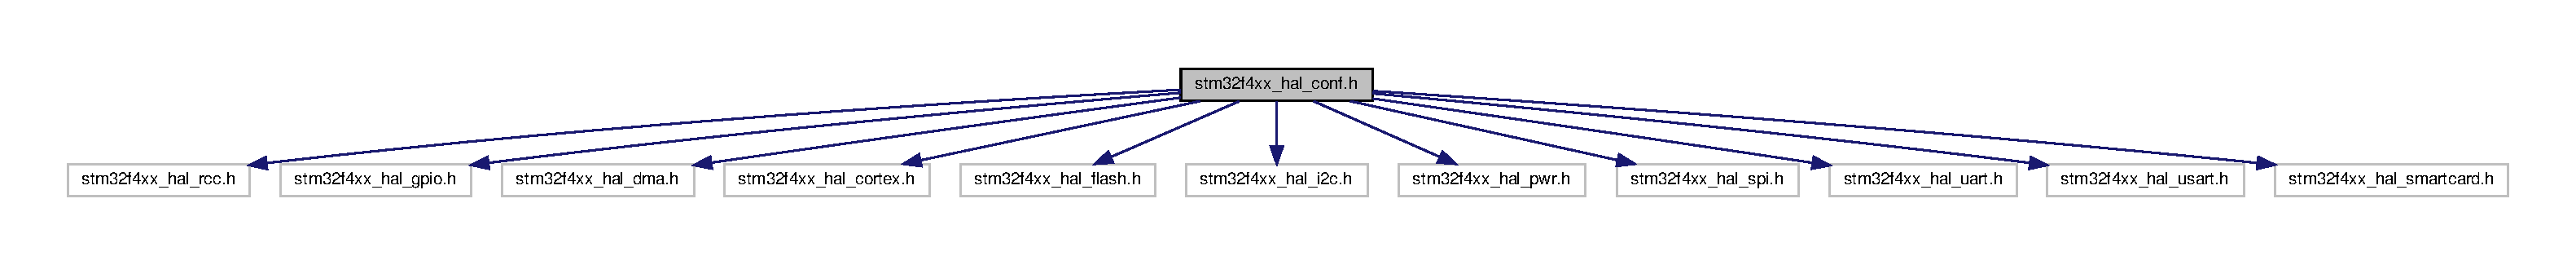
\includegraphics[width=350pt]{stm32f4xx__hal__conf_8h__incl}
\end{center}
\end{figure}
\subsection*{Macros}
\begin{DoxyCompactItemize}
\item 
\#define \hyperlink{stm32f4xx__hal__conf_8h_a877ae99e8c47a609ea97c888912bf75f}{H\+A\+L\+\_\+\+M\+O\+D\+U\+L\+E\+\_\+\+E\+N\+A\+B\+L\+ED}
\begin{DoxyCompactList}\small\item\em This is the list of modules to be used in the H\+AL driver. \end{DoxyCompactList}\item 
\#define \hyperlink{stm32f4xx__hal__conf_8h_a6552186102a1131b2849ac55a582945d}{H\+A\+L\+\_\+\+D\+M\+A\+\_\+\+M\+O\+D\+U\+L\+E\+\_\+\+E\+N\+A\+B\+L\+ED}
\item 
\#define \hyperlink{stm32f4xx__hal__conf_8h_a7112575efe3740911f19a13e6b170fee}{H\+A\+L\+\_\+\+F\+L\+A\+S\+H\+\_\+\+M\+O\+D\+U\+L\+E\+\_\+\+E\+N\+A\+B\+L\+ED}
\item 
\#define \hyperlink{stm32f4xx__hal__conf_8h_a86165f80d6078719ee0715afe13febf5}{H\+A\+L\+\_\+\+G\+P\+I\+O\+\_\+\+M\+O\+D\+U\+L\+E\+\_\+\+E\+N\+A\+B\+L\+ED}
\item 
\#define \hyperlink{stm32f4xx__hal__conf_8h_a19999766418b0224871f732d800841c6}{H\+A\+L\+\_\+\+I2\+C\+\_\+\+M\+O\+D\+U\+L\+E\+\_\+\+E\+N\+A\+B\+L\+ED}
\item 
\#define \hyperlink{stm32f4xx__hal__conf_8h_ab51923c3716977d7923f49cc9d081aa8}{H\+A\+L\+\_\+\+P\+W\+R\+\_\+\+M\+O\+D\+U\+L\+E\+\_\+\+E\+N\+A\+B\+L\+ED}
\item 
\#define \hyperlink{stm32f4xx__hal__conf_8h_ac3dd74314ed62ac8575e2f9f48b3ac48}{H\+A\+L\+\_\+\+R\+C\+C\+\_\+\+M\+O\+D\+U\+L\+E\+\_\+\+E\+N\+A\+B\+L\+ED}
\item 
\#define \hyperlink{stm32f4xx__hal__conf_8h_a8ad4712bf4add56892d057778e826e0c}{H\+A\+L\+\_\+\+S\+P\+I\+\_\+\+M\+O\+D\+U\+L\+E\+\_\+\+E\+N\+A\+B\+L\+ED}
\item 
\#define \hyperlink{stm32f4xx__hal__conf_8h_a167269406e73327b95c3bb7b9cfe6d89}{H\+A\+L\+\_\+\+U\+A\+R\+T\+\_\+\+M\+O\+D\+U\+L\+E\+\_\+\+E\+N\+A\+B\+L\+ED}
\item 
\#define \hyperlink{stm32f4xx__hal__conf_8h_adf2c524ff7f06b1d339e3173839fddec}{H\+A\+L\+\_\+\+U\+S\+A\+R\+T\+\_\+\+M\+O\+D\+U\+L\+E\+\_\+\+E\+N\+A\+B\+L\+ED}
\item 
\#define \hyperlink{stm32f4xx__hal__conf_8h_a2a5c5e3af52a068a158078c130345cf0}{H\+A\+L\+\_\+\+S\+M\+A\+R\+T\+C\+A\+R\+D\+\_\+\+M\+O\+D\+U\+L\+E\+\_\+\+E\+N\+A\+B\+L\+ED}
\item 
\#define \hyperlink{stm32f4xx__hal__conf_8h_aa9b5a3a425901e097de70092dbe31e0f}{H\+A\+L\+\_\+\+C\+O\+R\+T\+E\+X\+\_\+\+M\+O\+D\+U\+L\+E\+\_\+\+E\+N\+A\+B\+L\+ED}
\item 
\#define \hyperlink{stm32f4xx__hal__conf_8h_aeafcff4f57440c60e64812dddd13e7cb}{H\+S\+E\+\_\+\+V\+A\+L\+UE}~8000000U
\begin{DoxyCompactList}\small\item\em Adjust the value of External High Speed oscillator (H\+SE) used in your application. This value is used by the R\+CC H\+AL module to compute the system frequency (when H\+SE is used as system clock source, directly or through the P\+LL). \end{DoxyCompactList}\item 
\#define \hyperlink{stm32f4xx__hal__conf_8h_a68ecbc9b0a1a40a1ec9d18d5e9747c4f}{H\+S\+E\+\_\+\+S\+T\+A\+R\+T\+U\+P\+\_\+\+T\+I\+M\+E\+O\+UT}~100U
\item 
\#define \hyperlink{stm32f4xx__hal__conf_8h_aaa8c76e274d0f6dd2cefb5d0b17fbc37}{H\+S\+I\+\_\+\+V\+A\+L\+UE}~16000000U
\begin{DoxyCompactList}\small\item\em Internal High Speed oscillator (H\+SI) value. This value is used by the R\+CC H\+AL module to compute the system frequency (when H\+SI is used as system clock source, directly or through the P\+LL). \end{DoxyCompactList}\item 
\#define \hyperlink{stm32f4xx__hal__conf_8h_a4872023e65449c0506aac3ea6bec99e9}{L\+S\+I\+\_\+\+V\+A\+L\+UE}~32000U
\begin{DoxyCompactList}\small\item\em Internal Low Speed oscillator (L\+SI) value. \end{DoxyCompactList}\item 
\#define \hyperlink{stm32f4xx__hal__conf_8h_a7bbb9d19e5189a6ccd0fb6fa6177d20d}{L\+S\+E\+\_\+\+V\+A\+L\+UE}~32768U
\begin{DoxyCompactList}\small\item\em External Low Speed oscillator (L\+SE) value. \end{DoxyCompactList}\item 
\#define \hyperlink{stm32f4xx__hal__conf_8h_a85e6fc812dc26f7161a04be2568a5462}{L\+S\+E\+\_\+\+S\+T\+A\+R\+T\+U\+P\+\_\+\+T\+I\+M\+E\+O\+UT}~5000U
\item 
\#define \hyperlink{stm32f4xx__hal__conf_8h_a8c47c935e91e70569098b41718558648}{E\+X\+T\+E\+R\+N\+A\+L\+\_\+\+C\+L\+O\+C\+K\+\_\+\+V\+A\+L\+UE}~12288000U
\begin{DoxyCompactList}\small\item\em External clock source for I2S peripheral This value is used by the I2S H\+AL module to compute the I2S clock source frequency, this source is inserted directly through I2\+S\+\_\+\+C\+K\+IN pad. \end{DoxyCompactList}\item 
\#define \hyperlink{stm32f4xx__hal__conf_8h_aae550dad9f96d52cfce5e539adadbbb4}{V\+D\+D\+\_\+\+V\+A\+L\+UE}~3300U
\begin{DoxyCompactList}\small\item\em This is the H\+AL system configuration section. \end{DoxyCompactList}\item 
\#define \hyperlink{stm32f4xx__hal__conf_8h_ae27809d4959b9fd5b5d974e3e1c77d2e}{T\+I\+C\+K\+\_\+\+I\+N\+T\+\_\+\+P\+R\+I\+O\+R\+I\+TY}~0x0\+FU
\item 
\#define \hyperlink{stm32f4xx__hal__conf_8h_ad048ac737242c2c2cb9f4a72953d10ce}{U\+S\+E\+\_\+\+R\+T\+OS}~0U
\item 
\#define \hyperlink{stm32f4xx__hal__conf_8h_a13fc0d5e7bb925385c0cc0772ba6a391}{P\+R\+E\+F\+E\+T\+C\+H\+\_\+\+E\+N\+A\+B\+LE}~1U
\item 
\#define \hyperlink{stm32f4xx__hal__conf_8h_a3379989d46599c7e19a43f42e9145a4a}{I\+N\+S\+T\+R\+U\+C\+T\+I\+O\+N\+\_\+\+C\+A\+C\+H\+E\+\_\+\+E\+N\+A\+B\+LE}~1U
\item 
\#define \hyperlink{stm32f4xx__hal__conf_8h_a5b4c32a40cf49b06c0d761e385949a6b}{D\+A\+T\+A\+\_\+\+C\+A\+C\+H\+E\+\_\+\+E\+N\+A\+B\+LE}~1U
\item 
\#define \hyperlink{stm32f4xx__hal__conf_8h_ab84a2e15d360e2644ada09641513a941}{M\+A\+C\+\_\+\+A\+D\+D\+R0}~2U
\begin{DoxyCompactList}\small\item\em Uncomment the line below to expanse the \char`\"{}assert\+\_\+param\char`\"{} macro in the H\+AL drivers code. \end{DoxyCompactList}\item 
\#define \hyperlink{stm32f4xx__hal__conf_8h_a8d14266d76690c530bee01e7e5bb4099}{M\+A\+C\+\_\+\+A\+D\+D\+R1}~0U
\item 
\#define \hyperlink{stm32f4xx__hal__conf_8h_a6c5df15bec1d305ed033ad9a85ec803d}{M\+A\+C\+\_\+\+A\+D\+D\+R2}~0U
\item 
\#define \hyperlink{stm32f4xx__hal__conf_8h_a08a36ede83ae67498aecf54676be8fc8}{M\+A\+C\+\_\+\+A\+D\+D\+R3}~0U
\item 
\#define \hyperlink{stm32f4xx__hal__conf_8h_a41e5cb0b39ad74f0aafb83dbcecf9006}{M\+A\+C\+\_\+\+A\+D\+D\+R4}~0U
\item 
\#define \hyperlink{stm32f4xx__hal__conf_8h_a3bcc92663c42ec434f527847bbc4abc1}{M\+A\+C\+\_\+\+A\+D\+D\+R5}~0U
\item 
\#define \hyperlink{stm32f4xx__hal__conf_8h_a0cdaf687f7a7f2dba570d5a722990786}{E\+T\+H\+\_\+\+R\+X\+\_\+\+B\+U\+F\+\_\+\+S\+I\+ZE}~E\+T\+H\+\_\+\+M\+A\+X\+\_\+\+P\+A\+C\+K\+E\+T\+\_\+\+S\+I\+ZE /$\ast$ buffer size for receive               $\ast$/
\item 
\#define \hyperlink{stm32f4xx__hal__conf_8h_af83956dfc1b135c3c92ac409758b6cf4}{E\+T\+H\+\_\+\+T\+X\+\_\+\+B\+U\+F\+\_\+\+S\+I\+ZE}~E\+T\+H\+\_\+\+M\+A\+X\+\_\+\+P\+A\+C\+K\+E\+T\+\_\+\+S\+I\+ZE /$\ast$ buffer size for transmit              $\ast$/
\item 
\#define \hyperlink{stm32f4xx__hal__conf_8h_a62b0f224fa9c4f2e5574c9e52526f751}{E\+T\+H\+\_\+\+R\+X\+B\+U\+F\+NB}~4\+U                  /$\ast$ 4 Rx buffers of size E\+T\+H\+\_\+\+R\+X\+\_\+\+B\+U\+F\+\_\+\+S\+I\+Z\+E  $\ast$/
\item 
\#define \hyperlink{stm32f4xx__hal__conf_8h_a4ad07ad8fa6f8639ab8ef362390d86c7}{E\+T\+H\+\_\+\+T\+X\+B\+U\+F\+NB}~4\+U                  /$\ast$ 4 Tx buffers of size E\+T\+H\+\_\+\+T\+X\+\_\+\+B\+U\+F\+\_\+\+S\+I\+Z\+E  $\ast$/
\item 
\#define \hyperlink{stm32f4xx__hal__conf_8h_a25f014091aaba92bdd9d95d0b2f00503}{D\+P83848\+\_\+\+P\+H\+Y\+\_\+\+A\+D\+D\+R\+E\+SS}~0x01U
\item 
\#define \hyperlink{stm32f4xx__hal__conf_8h_a0ede6087f7b71403bcddb5d3a8f47ff4}{P\+H\+Y\+\_\+\+R\+E\+S\+E\+T\+\_\+\+D\+E\+L\+AY}~0x000000\+F\+FU
\item 
\#define \hyperlink{stm32f4xx__hal__conf_8h_abba7114255a2a41b81fdcb2a3702c270}{P\+H\+Y\+\_\+\+C\+O\+N\+F\+I\+G\+\_\+\+D\+E\+L\+AY}~0x00000\+F\+F\+FU
\item 
\#define \hyperlink{stm32f4xx__hal__conf_8h_a9d356ada86535630c403690bef0fb887}{P\+H\+Y\+\_\+\+R\+E\+A\+D\+\_\+\+TO}~0x0000\+F\+F\+F\+FU
\item 
\#define \hyperlink{stm32f4xx__hal__conf_8h_a474bf13e28d09b667e41b151140ee39d}{P\+H\+Y\+\_\+\+W\+R\+I\+T\+E\+\_\+\+TO}~0x0000\+F\+F\+F\+FU
\item 
\#define \hyperlink{stm32f4xx__hal__conf_8h_a8abe1a40c71e68881ec669d59f513fdb}{P\+H\+Y\+\_\+\+B\+CR}~((uint16\+\_\+t)0x0000)
\item 
\#define \hyperlink{stm32f4xx__hal__conf_8h_a4b8f2c29a9e74412395e1b1809666838}{P\+H\+Y\+\_\+\+B\+SR}~((uint16\+\_\+t)0x0001)
\item 
\#define \hyperlink{stm32f4xx__hal__conf_8h_a6f5048620b3dde8583f7f1118e9de187}{P\+H\+Y\+\_\+\+R\+E\+S\+ET}~((uint16\+\_\+t)0x8000)
\item 
\#define \hyperlink{stm32f4xx__hal__conf_8h_a7833d885caa7e29abbebfb90a4b96f86}{P\+H\+Y\+\_\+\+L\+O\+O\+P\+B\+A\+CK}~((uint16\+\_\+t)0x4000)
\item 
\#define \hyperlink{stm32f4xx__hal__conf_8h_a5729771244f68779fc694ba819cd60a5}{P\+H\+Y\+\_\+\+F\+U\+L\+L\+D\+U\+P\+L\+E\+X\+\_\+100M}~((uint16\+\_\+t)0x2100)
\item 
\#define \hyperlink{stm32f4xx__hal__conf_8h_a1ac901a4ad405241d90a5c10104b8986}{P\+H\+Y\+\_\+\+H\+A\+L\+F\+D\+U\+P\+L\+E\+X\+\_\+100M}~((uint16\+\_\+t)0x2000)
\item 
\#define \hyperlink{stm32f4xx__hal__conf_8h_a6b6254fd3dacbf1578a9d8058cd86373}{P\+H\+Y\+\_\+\+F\+U\+L\+L\+D\+U\+P\+L\+E\+X\+\_\+10M}~((uint16\+\_\+t)0x0100)
\item 
\#define \hyperlink{stm32f4xx__hal__conf_8h_a4fa7ca6faf60ee074576ebb6103f8dd4}{P\+H\+Y\+\_\+\+H\+A\+L\+F\+D\+U\+P\+L\+E\+X\+\_\+10M}~((uint16\+\_\+t)0x0000)
\item 
\#define \hyperlink{stm32f4xx__hal__conf_8h_a9b7f5c8f71047ee449f21562d26b1b43}{P\+H\+Y\+\_\+\+A\+U\+T\+O\+N\+E\+G\+O\+T\+I\+A\+T\+I\+ON}~((uint16\+\_\+t)0x1000)
\item 
\#define \hyperlink{stm32f4xx__hal__conf_8h_a66c4b69bd08dc25b6730365d3ff740c9}{P\+H\+Y\+\_\+\+R\+E\+S\+T\+A\+R\+T\+\_\+\+A\+U\+T\+O\+N\+E\+G\+O\+T\+I\+A\+T\+I\+ON}~((uint16\+\_\+t)0x0200)
\item 
\#define \hyperlink{stm32f4xx__hal__conf_8h_aa0b1e6d4a23470fc1ac4f9222b51f8a0}{P\+H\+Y\+\_\+\+P\+O\+W\+E\+R\+D\+O\+WN}~((uint16\+\_\+t)0x0800)
\item 
\#define \hyperlink{stm32f4xx__hal__conf_8h_a7d5233295134a385866eb5bdafe2162b}{P\+H\+Y\+\_\+\+I\+S\+O\+L\+A\+TE}~((uint16\+\_\+t)0x0400)
\item 
\#define \hyperlink{stm32f4xx__hal__conf_8h_a36c4dbd5f6df1f5eaefa010929ef9773}{P\+H\+Y\+\_\+\+A\+U\+T\+O\+N\+E\+G\+O\+\_\+\+C\+O\+M\+P\+L\+E\+TE}~((uint16\+\_\+t)0x0020)
\item 
\#define \hyperlink{stm32f4xx__hal__conf_8h_ace209074499dbef0b97300da5bd7c707}{P\+H\+Y\+\_\+\+L\+I\+N\+K\+E\+D\+\_\+\+S\+T\+A\+T\+US}~((uint16\+\_\+t)0x0004)
\item 
\#define \hyperlink{stm32f4xx__hal__conf_8h_a057b4d3fb66548d65c291a5b41611be2}{P\+H\+Y\+\_\+\+J\+A\+B\+B\+E\+R\+\_\+\+D\+E\+T\+E\+C\+T\+I\+ON}~((uint16\+\_\+t)0x0002)
\item 
\#define \hyperlink{stm32f4xx__hal__conf_8h_a32b55e84d27cf298a77f54b133cd1acc}{P\+H\+Y\+\_\+\+SR}~((uint16\+\_\+t)0x0010)
\item 
\#define \hyperlink{stm32f4xx__hal__conf_8h_ac4d8c2e6c2509a9bdaf214b24deafea7}{P\+H\+Y\+\_\+\+M\+I\+CR}~((uint16\+\_\+t)0x0011)
\item 
\#define \hyperlink{stm32f4xx__hal__conf_8h_a81d36e97e4a9da33f2a7e142b01964f6}{P\+H\+Y\+\_\+\+M\+I\+SR}~((uint16\+\_\+t)0x0012)
\item 
\#define \hyperlink{stm32f4xx__hal__conf_8h_a4a6cbf61f5e1a134d8983ef29fd2d386}{P\+H\+Y\+\_\+\+L\+I\+N\+K\+\_\+\+S\+T\+A\+T\+US}~((uint16\+\_\+t)0x0001)
\item 
\#define \hyperlink{stm32f4xx__hal__conf_8h_a74c081bc55e9ff96bf229f44e96c6155}{P\+H\+Y\+\_\+\+S\+P\+E\+E\+D\+\_\+\+S\+T\+A\+T\+US}~((uint16\+\_\+t)0x0002)
\item 
\#define \hyperlink{stm32f4xx__hal__conf_8h_ab928f45585242fde1a8d81a2d9ed22d0}{P\+H\+Y\+\_\+\+D\+U\+P\+L\+E\+X\+\_\+\+S\+T\+A\+T\+US}~((uint16\+\_\+t)0x0004)
\item 
\#define \hyperlink{stm32f4xx__hal__conf_8h_ab0314b8559d5895194b435ae93aee9c9}{P\+H\+Y\+\_\+\+M\+I\+C\+R\+\_\+\+I\+N\+T\+\_\+\+EN}~((uint16\+\_\+t)0x0002)
\item 
\#define \hyperlink{stm32f4xx__hal__conf_8h_aca1bf9e00caba70caa1f1a9e56cbee5c}{P\+H\+Y\+\_\+\+M\+I\+C\+R\+\_\+\+I\+N\+T\+\_\+\+OE}~((uint16\+\_\+t)0x0001)
\item 
\#define \hyperlink{stm32f4xx__hal__conf_8h_aaf06885683edcd946ad960f59e8a6f9a}{P\+H\+Y\+\_\+\+M\+I\+S\+R\+\_\+\+L\+I\+N\+K\+\_\+\+I\+N\+T\+\_\+\+EN}~((uint16\+\_\+t)0x0020)
\item 
\#define \hyperlink{stm32f4xx__hal__conf_8h_a7c378eb26673981df0834658f4fec4c1}{P\+H\+Y\+\_\+\+L\+I\+N\+K\+\_\+\+I\+N\+T\+E\+R\+R\+U\+PT}~((uint16\+\_\+t)0x2000)
\item 
\#define \hyperlink{stm32f4xx__hal__conf_8h_a4c6fab687afc7ba4469b1b2d34472358}{U\+S\+E\+\_\+\+S\+P\+I\+\_\+\+C\+RC}~1U
\item 
\#define \hyperlink{stm32f4xx__hal__conf_8h_a631dea7b230e600555f979c62af1de21}{assert\+\_\+param}(expr)~((void)0\+U)
\begin{DoxyCompactList}\small\item\em Include module\textquotesingle{}s header file. \end{DoxyCompactList}\end{DoxyCompactItemize}


\subsection{Macro Definition Documentation}
\mbox{\Hypertarget{stm32f4xx__hal__conf_8h_a631dea7b230e600555f979c62af1de21}\label{stm32f4xx__hal__conf_8h_a631dea7b230e600555f979c62af1de21}} 
\index{stm32f4xx\+\_\+hal\+\_\+conf.\+h@{stm32f4xx\+\_\+hal\+\_\+conf.\+h}!assert\+\_\+param@{assert\+\_\+param}}
\index{assert\+\_\+param@{assert\+\_\+param}!stm32f4xx\+\_\+hal\+\_\+conf.\+h@{stm32f4xx\+\_\+hal\+\_\+conf.\+h}}
\subsubsection{\texorpdfstring{assert\+\_\+param}{assert\_param}}
{\footnotesize\ttfamily \#define assert\+\_\+param(\begin{DoxyParamCaption}\item[{}]{expr }\end{DoxyParamCaption})~((void)0\+U)}



Include module\textquotesingle{}s header file. 

\mbox{\Hypertarget{stm32f4xx__hal__conf_8h_a5b4c32a40cf49b06c0d761e385949a6b}\label{stm32f4xx__hal__conf_8h_a5b4c32a40cf49b06c0d761e385949a6b}} 
\index{stm32f4xx\+\_\+hal\+\_\+conf.\+h@{stm32f4xx\+\_\+hal\+\_\+conf.\+h}!D\+A\+T\+A\+\_\+\+C\+A\+C\+H\+E\+\_\+\+E\+N\+A\+B\+LE@{D\+A\+T\+A\+\_\+\+C\+A\+C\+H\+E\+\_\+\+E\+N\+A\+B\+LE}}
\index{D\+A\+T\+A\+\_\+\+C\+A\+C\+H\+E\+\_\+\+E\+N\+A\+B\+LE@{D\+A\+T\+A\+\_\+\+C\+A\+C\+H\+E\+\_\+\+E\+N\+A\+B\+LE}!stm32f4xx\+\_\+hal\+\_\+conf.\+h@{stm32f4xx\+\_\+hal\+\_\+conf.\+h}}
\subsubsection{\texorpdfstring{D\+A\+T\+A\+\_\+\+C\+A\+C\+H\+E\+\_\+\+E\+N\+A\+B\+LE}{DATA\_CACHE\_ENABLE}}
{\footnotesize\ttfamily \#define D\+A\+T\+A\+\_\+\+C\+A\+C\+H\+E\+\_\+\+E\+N\+A\+B\+LE~1U}

\mbox{\Hypertarget{stm32f4xx__hal__conf_8h_a25f014091aaba92bdd9d95d0b2f00503}\label{stm32f4xx__hal__conf_8h_a25f014091aaba92bdd9d95d0b2f00503}} 
\index{stm32f4xx\+\_\+hal\+\_\+conf.\+h@{stm32f4xx\+\_\+hal\+\_\+conf.\+h}!D\+P83848\+\_\+\+P\+H\+Y\+\_\+\+A\+D\+D\+R\+E\+SS@{D\+P83848\+\_\+\+P\+H\+Y\+\_\+\+A\+D\+D\+R\+E\+SS}}
\index{D\+P83848\+\_\+\+P\+H\+Y\+\_\+\+A\+D\+D\+R\+E\+SS@{D\+P83848\+\_\+\+P\+H\+Y\+\_\+\+A\+D\+D\+R\+E\+SS}!stm32f4xx\+\_\+hal\+\_\+conf.\+h@{stm32f4xx\+\_\+hal\+\_\+conf.\+h}}
\subsubsection{\texorpdfstring{D\+P83848\+\_\+\+P\+H\+Y\+\_\+\+A\+D\+D\+R\+E\+SS}{DP83848\_PHY\_ADDRESS}}
{\footnotesize\ttfamily \#define D\+P83848\+\_\+\+P\+H\+Y\+\_\+\+A\+D\+D\+R\+E\+SS~0x01U}

\mbox{\Hypertarget{stm32f4xx__hal__conf_8h_a0cdaf687f7a7f2dba570d5a722990786}\label{stm32f4xx__hal__conf_8h_a0cdaf687f7a7f2dba570d5a722990786}} 
\index{stm32f4xx\+\_\+hal\+\_\+conf.\+h@{stm32f4xx\+\_\+hal\+\_\+conf.\+h}!E\+T\+H\+\_\+\+R\+X\+\_\+\+B\+U\+F\+\_\+\+S\+I\+ZE@{E\+T\+H\+\_\+\+R\+X\+\_\+\+B\+U\+F\+\_\+\+S\+I\+ZE}}
\index{E\+T\+H\+\_\+\+R\+X\+\_\+\+B\+U\+F\+\_\+\+S\+I\+ZE@{E\+T\+H\+\_\+\+R\+X\+\_\+\+B\+U\+F\+\_\+\+S\+I\+ZE}!stm32f4xx\+\_\+hal\+\_\+conf.\+h@{stm32f4xx\+\_\+hal\+\_\+conf.\+h}}
\subsubsection{\texorpdfstring{E\+T\+H\+\_\+\+R\+X\+\_\+\+B\+U\+F\+\_\+\+S\+I\+ZE}{ETH\_RX\_BUF\_SIZE}}
{\footnotesize\ttfamily \#define E\+T\+H\+\_\+\+R\+X\+\_\+\+B\+U\+F\+\_\+\+S\+I\+ZE~E\+T\+H\+\_\+\+M\+A\+X\+\_\+\+P\+A\+C\+K\+E\+T\+\_\+\+S\+I\+ZE /$\ast$ buffer size for receive               $\ast$/}

\mbox{\Hypertarget{stm32f4xx__hal__conf_8h_a62b0f224fa9c4f2e5574c9e52526f751}\label{stm32f4xx__hal__conf_8h_a62b0f224fa9c4f2e5574c9e52526f751}} 
\index{stm32f4xx\+\_\+hal\+\_\+conf.\+h@{stm32f4xx\+\_\+hal\+\_\+conf.\+h}!E\+T\+H\+\_\+\+R\+X\+B\+U\+F\+NB@{E\+T\+H\+\_\+\+R\+X\+B\+U\+F\+NB}}
\index{E\+T\+H\+\_\+\+R\+X\+B\+U\+F\+NB@{E\+T\+H\+\_\+\+R\+X\+B\+U\+F\+NB}!stm32f4xx\+\_\+hal\+\_\+conf.\+h@{stm32f4xx\+\_\+hal\+\_\+conf.\+h}}
\subsubsection{\texorpdfstring{E\+T\+H\+\_\+\+R\+X\+B\+U\+F\+NB}{ETH\_RXBUFNB}}
{\footnotesize\ttfamily \#define E\+T\+H\+\_\+\+R\+X\+B\+U\+F\+NB~4\+U                  /$\ast$ 4 Rx buffers of size E\+T\+H\+\_\+\+R\+X\+\_\+\+B\+U\+F\+\_\+\+S\+I\+Z\+E  $\ast$/}

\mbox{\Hypertarget{stm32f4xx__hal__conf_8h_af83956dfc1b135c3c92ac409758b6cf4}\label{stm32f4xx__hal__conf_8h_af83956dfc1b135c3c92ac409758b6cf4}} 
\index{stm32f4xx\+\_\+hal\+\_\+conf.\+h@{stm32f4xx\+\_\+hal\+\_\+conf.\+h}!E\+T\+H\+\_\+\+T\+X\+\_\+\+B\+U\+F\+\_\+\+S\+I\+ZE@{E\+T\+H\+\_\+\+T\+X\+\_\+\+B\+U\+F\+\_\+\+S\+I\+ZE}}
\index{E\+T\+H\+\_\+\+T\+X\+\_\+\+B\+U\+F\+\_\+\+S\+I\+ZE@{E\+T\+H\+\_\+\+T\+X\+\_\+\+B\+U\+F\+\_\+\+S\+I\+ZE}!stm32f4xx\+\_\+hal\+\_\+conf.\+h@{stm32f4xx\+\_\+hal\+\_\+conf.\+h}}
\subsubsection{\texorpdfstring{E\+T\+H\+\_\+\+T\+X\+\_\+\+B\+U\+F\+\_\+\+S\+I\+ZE}{ETH\_TX\_BUF\_SIZE}}
{\footnotesize\ttfamily \#define E\+T\+H\+\_\+\+T\+X\+\_\+\+B\+U\+F\+\_\+\+S\+I\+ZE~E\+T\+H\+\_\+\+M\+A\+X\+\_\+\+P\+A\+C\+K\+E\+T\+\_\+\+S\+I\+ZE /$\ast$ buffer size for transmit              $\ast$/}

\mbox{\Hypertarget{stm32f4xx__hal__conf_8h_a4ad07ad8fa6f8639ab8ef362390d86c7}\label{stm32f4xx__hal__conf_8h_a4ad07ad8fa6f8639ab8ef362390d86c7}} 
\index{stm32f4xx\+\_\+hal\+\_\+conf.\+h@{stm32f4xx\+\_\+hal\+\_\+conf.\+h}!E\+T\+H\+\_\+\+T\+X\+B\+U\+F\+NB@{E\+T\+H\+\_\+\+T\+X\+B\+U\+F\+NB}}
\index{E\+T\+H\+\_\+\+T\+X\+B\+U\+F\+NB@{E\+T\+H\+\_\+\+T\+X\+B\+U\+F\+NB}!stm32f4xx\+\_\+hal\+\_\+conf.\+h@{stm32f4xx\+\_\+hal\+\_\+conf.\+h}}
\subsubsection{\texorpdfstring{E\+T\+H\+\_\+\+T\+X\+B\+U\+F\+NB}{ETH\_TXBUFNB}}
{\footnotesize\ttfamily \#define E\+T\+H\+\_\+\+T\+X\+B\+U\+F\+NB~4\+U                  /$\ast$ 4 Tx buffers of size E\+T\+H\+\_\+\+T\+X\+\_\+\+B\+U\+F\+\_\+\+S\+I\+Z\+E  $\ast$/}

\mbox{\Hypertarget{stm32f4xx__hal__conf_8h_a8c47c935e91e70569098b41718558648}\label{stm32f4xx__hal__conf_8h_a8c47c935e91e70569098b41718558648}} 
\index{stm32f4xx\+\_\+hal\+\_\+conf.\+h@{stm32f4xx\+\_\+hal\+\_\+conf.\+h}!E\+X\+T\+E\+R\+N\+A\+L\+\_\+\+C\+L\+O\+C\+K\+\_\+\+V\+A\+L\+UE@{E\+X\+T\+E\+R\+N\+A\+L\+\_\+\+C\+L\+O\+C\+K\+\_\+\+V\+A\+L\+UE}}
\index{E\+X\+T\+E\+R\+N\+A\+L\+\_\+\+C\+L\+O\+C\+K\+\_\+\+V\+A\+L\+UE@{E\+X\+T\+E\+R\+N\+A\+L\+\_\+\+C\+L\+O\+C\+K\+\_\+\+V\+A\+L\+UE}!stm32f4xx\+\_\+hal\+\_\+conf.\+h@{stm32f4xx\+\_\+hal\+\_\+conf.\+h}}
\subsubsection{\texorpdfstring{E\+X\+T\+E\+R\+N\+A\+L\+\_\+\+C\+L\+O\+C\+K\+\_\+\+V\+A\+L\+UE}{EXTERNAL\_CLOCK\_VALUE}}
{\footnotesize\ttfamily \#define E\+X\+T\+E\+R\+N\+A\+L\+\_\+\+C\+L\+O\+C\+K\+\_\+\+V\+A\+L\+UE~12288000U}



External clock source for I2S peripheral This value is used by the I2S H\+AL module to compute the I2S clock source frequency, this source is inserted directly through I2\+S\+\_\+\+C\+K\+IN pad. 

Value of the External oscillator in Hz \mbox{\Hypertarget{stm32f4xx__hal__conf_8h_aa9b5a3a425901e097de70092dbe31e0f}\label{stm32f4xx__hal__conf_8h_aa9b5a3a425901e097de70092dbe31e0f}} 
\index{stm32f4xx\+\_\+hal\+\_\+conf.\+h@{stm32f4xx\+\_\+hal\+\_\+conf.\+h}!H\+A\+L\+\_\+\+C\+O\+R\+T\+E\+X\+\_\+\+M\+O\+D\+U\+L\+E\+\_\+\+E\+N\+A\+B\+L\+ED@{H\+A\+L\+\_\+\+C\+O\+R\+T\+E\+X\+\_\+\+M\+O\+D\+U\+L\+E\+\_\+\+E\+N\+A\+B\+L\+ED}}
\index{H\+A\+L\+\_\+\+C\+O\+R\+T\+E\+X\+\_\+\+M\+O\+D\+U\+L\+E\+\_\+\+E\+N\+A\+B\+L\+ED@{H\+A\+L\+\_\+\+C\+O\+R\+T\+E\+X\+\_\+\+M\+O\+D\+U\+L\+E\+\_\+\+E\+N\+A\+B\+L\+ED}!stm32f4xx\+\_\+hal\+\_\+conf.\+h@{stm32f4xx\+\_\+hal\+\_\+conf.\+h}}
\subsubsection{\texorpdfstring{H\+A\+L\+\_\+\+C\+O\+R\+T\+E\+X\+\_\+\+M\+O\+D\+U\+L\+E\+\_\+\+E\+N\+A\+B\+L\+ED}{HAL\_CORTEX\_MODULE\_ENABLED}}
{\footnotesize\ttfamily \#define H\+A\+L\+\_\+\+C\+O\+R\+T\+E\+X\+\_\+\+M\+O\+D\+U\+L\+E\+\_\+\+E\+N\+A\+B\+L\+ED}

\mbox{\Hypertarget{stm32f4xx__hal__conf_8h_a6552186102a1131b2849ac55a582945d}\label{stm32f4xx__hal__conf_8h_a6552186102a1131b2849ac55a582945d}} 
\index{stm32f4xx\+\_\+hal\+\_\+conf.\+h@{stm32f4xx\+\_\+hal\+\_\+conf.\+h}!H\+A\+L\+\_\+\+D\+M\+A\+\_\+\+M\+O\+D\+U\+L\+E\+\_\+\+E\+N\+A\+B\+L\+ED@{H\+A\+L\+\_\+\+D\+M\+A\+\_\+\+M\+O\+D\+U\+L\+E\+\_\+\+E\+N\+A\+B\+L\+ED}}
\index{H\+A\+L\+\_\+\+D\+M\+A\+\_\+\+M\+O\+D\+U\+L\+E\+\_\+\+E\+N\+A\+B\+L\+ED@{H\+A\+L\+\_\+\+D\+M\+A\+\_\+\+M\+O\+D\+U\+L\+E\+\_\+\+E\+N\+A\+B\+L\+ED}!stm32f4xx\+\_\+hal\+\_\+conf.\+h@{stm32f4xx\+\_\+hal\+\_\+conf.\+h}}
\subsubsection{\texorpdfstring{H\+A\+L\+\_\+\+D\+M\+A\+\_\+\+M\+O\+D\+U\+L\+E\+\_\+\+E\+N\+A\+B\+L\+ED}{HAL\_DMA\_MODULE\_ENABLED}}
{\footnotesize\ttfamily \#define H\+A\+L\+\_\+\+D\+M\+A\+\_\+\+M\+O\+D\+U\+L\+E\+\_\+\+E\+N\+A\+B\+L\+ED}

\mbox{\Hypertarget{stm32f4xx__hal__conf_8h_a7112575efe3740911f19a13e6b170fee}\label{stm32f4xx__hal__conf_8h_a7112575efe3740911f19a13e6b170fee}} 
\index{stm32f4xx\+\_\+hal\+\_\+conf.\+h@{stm32f4xx\+\_\+hal\+\_\+conf.\+h}!H\+A\+L\+\_\+\+F\+L\+A\+S\+H\+\_\+\+M\+O\+D\+U\+L\+E\+\_\+\+E\+N\+A\+B\+L\+ED@{H\+A\+L\+\_\+\+F\+L\+A\+S\+H\+\_\+\+M\+O\+D\+U\+L\+E\+\_\+\+E\+N\+A\+B\+L\+ED}}
\index{H\+A\+L\+\_\+\+F\+L\+A\+S\+H\+\_\+\+M\+O\+D\+U\+L\+E\+\_\+\+E\+N\+A\+B\+L\+ED@{H\+A\+L\+\_\+\+F\+L\+A\+S\+H\+\_\+\+M\+O\+D\+U\+L\+E\+\_\+\+E\+N\+A\+B\+L\+ED}!stm32f4xx\+\_\+hal\+\_\+conf.\+h@{stm32f4xx\+\_\+hal\+\_\+conf.\+h}}
\subsubsection{\texorpdfstring{H\+A\+L\+\_\+\+F\+L\+A\+S\+H\+\_\+\+M\+O\+D\+U\+L\+E\+\_\+\+E\+N\+A\+B\+L\+ED}{HAL\_FLASH\_MODULE\_ENABLED}}
{\footnotesize\ttfamily \#define H\+A\+L\+\_\+\+F\+L\+A\+S\+H\+\_\+\+M\+O\+D\+U\+L\+E\+\_\+\+E\+N\+A\+B\+L\+ED}

\mbox{\Hypertarget{stm32f4xx__hal__conf_8h_a86165f80d6078719ee0715afe13febf5}\label{stm32f4xx__hal__conf_8h_a86165f80d6078719ee0715afe13febf5}} 
\index{stm32f4xx\+\_\+hal\+\_\+conf.\+h@{stm32f4xx\+\_\+hal\+\_\+conf.\+h}!H\+A\+L\+\_\+\+G\+P\+I\+O\+\_\+\+M\+O\+D\+U\+L\+E\+\_\+\+E\+N\+A\+B\+L\+ED@{H\+A\+L\+\_\+\+G\+P\+I\+O\+\_\+\+M\+O\+D\+U\+L\+E\+\_\+\+E\+N\+A\+B\+L\+ED}}
\index{H\+A\+L\+\_\+\+G\+P\+I\+O\+\_\+\+M\+O\+D\+U\+L\+E\+\_\+\+E\+N\+A\+B\+L\+ED@{H\+A\+L\+\_\+\+G\+P\+I\+O\+\_\+\+M\+O\+D\+U\+L\+E\+\_\+\+E\+N\+A\+B\+L\+ED}!stm32f4xx\+\_\+hal\+\_\+conf.\+h@{stm32f4xx\+\_\+hal\+\_\+conf.\+h}}
\subsubsection{\texorpdfstring{H\+A\+L\+\_\+\+G\+P\+I\+O\+\_\+\+M\+O\+D\+U\+L\+E\+\_\+\+E\+N\+A\+B\+L\+ED}{HAL\_GPIO\_MODULE\_ENABLED}}
{\footnotesize\ttfamily \#define H\+A\+L\+\_\+\+G\+P\+I\+O\+\_\+\+M\+O\+D\+U\+L\+E\+\_\+\+E\+N\+A\+B\+L\+ED}

\mbox{\Hypertarget{stm32f4xx__hal__conf_8h_a19999766418b0224871f732d800841c6}\label{stm32f4xx__hal__conf_8h_a19999766418b0224871f732d800841c6}} 
\index{stm32f4xx\+\_\+hal\+\_\+conf.\+h@{stm32f4xx\+\_\+hal\+\_\+conf.\+h}!H\+A\+L\+\_\+\+I2\+C\+\_\+\+M\+O\+D\+U\+L\+E\+\_\+\+E\+N\+A\+B\+L\+ED@{H\+A\+L\+\_\+\+I2\+C\+\_\+\+M\+O\+D\+U\+L\+E\+\_\+\+E\+N\+A\+B\+L\+ED}}
\index{H\+A\+L\+\_\+\+I2\+C\+\_\+\+M\+O\+D\+U\+L\+E\+\_\+\+E\+N\+A\+B\+L\+ED@{H\+A\+L\+\_\+\+I2\+C\+\_\+\+M\+O\+D\+U\+L\+E\+\_\+\+E\+N\+A\+B\+L\+ED}!stm32f4xx\+\_\+hal\+\_\+conf.\+h@{stm32f4xx\+\_\+hal\+\_\+conf.\+h}}
\subsubsection{\texorpdfstring{H\+A\+L\+\_\+\+I2\+C\+\_\+\+M\+O\+D\+U\+L\+E\+\_\+\+E\+N\+A\+B\+L\+ED}{HAL\_I2C\_MODULE\_ENABLED}}
{\footnotesize\ttfamily \#define H\+A\+L\+\_\+\+I2\+C\+\_\+\+M\+O\+D\+U\+L\+E\+\_\+\+E\+N\+A\+B\+L\+ED}

\mbox{\Hypertarget{stm32f4xx__hal__conf_8h_a877ae99e8c47a609ea97c888912bf75f}\label{stm32f4xx__hal__conf_8h_a877ae99e8c47a609ea97c888912bf75f}} 
\index{stm32f4xx\+\_\+hal\+\_\+conf.\+h@{stm32f4xx\+\_\+hal\+\_\+conf.\+h}!H\+A\+L\+\_\+\+M\+O\+D\+U\+L\+E\+\_\+\+E\+N\+A\+B\+L\+ED@{H\+A\+L\+\_\+\+M\+O\+D\+U\+L\+E\+\_\+\+E\+N\+A\+B\+L\+ED}}
\index{H\+A\+L\+\_\+\+M\+O\+D\+U\+L\+E\+\_\+\+E\+N\+A\+B\+L\+ED@{H\+A\+L\+\_\+\+M\+O\+D\+U\+L\+E\+\_\+\+E\+N\+A\+B\+L\+ED}!stm32f4xx\+\_\+hal\+\_\+conf.\+h@{stm32f4xx\+\_\+hal\+\_\+conf.\+h}}
\subsubsection{\texorpdfstring{H\+A\+L\+\_\+\+M\+O\+D\+U\+L\+E\+\_\+\+E\+N\+A\+B\+L\+ED}{HAL\_MODULE\_ENABLED}}
{\footnotesize\ttfamily \#define H\+A\+L\+\_\+\+M\+O\+D\+U\+L\+E\+\_\+\+E\+N\+A\+B\+L\+ED}



This is the list of modules to be used in the H\+AL driver. 

\mbox{\Hypertarget{stm32f4xx__hal__conf_8h_ab51923c3716977d7923f49cc9d081aa8}\label{stm32f4xx__hal__conf_8h_ab51923c3716977d7923f49cc9d081aa8}} 
\index{stm32f4xx\+\_\+hal\+\_\+conf.\+h@{stm32f4xx\+\_\+hal\+\_\+conf.\+h}!H\+A\+L\+\_\+\+P\+W\+R\+\_\+\+M\+O\+D\+U\+L\+E\+\_\+\+E\+N\+A\+B\+L\+ED@{H\+A\+L\+\_\+\+P\+W\+R\+\_\+\+M\+O\+D\+U\+L\+E\+\_\+\+E\+N\+A\+B\+L\+ED}}
\index{H\+A\+L\+\_\+\+P\+W\+R\+\_\+\+M\+O\+D\+U\+L\+E\+\_\+\+E\+N\+A\+B\+L\+ED@{H\+A\+L\+\_\+\+P\+W\+R\+\_\+\+M\+O\+D\+U\+L\+E\+\_\+\+E\+N\+A\+B\+L\+ED}!stm32f4xx\+\_\+hal\+\_\+conf.\+h@{stm32f4xx\+\_\+hal\+\_\+conf.\+h}}
\subsubsection{\texorpdfstring{H\+A\+L\+\_\+\+P\+W\+R\+\_\+\+M\+O\+D\+U\+L\+E\+\_\+\+E\+N\+A\+B\+L\+ED}{HAL\_PWR\_MODULE\_ENABLED}}
{\footnotesize\ttfamily \#define H\+A\+L\+\_\+\+P\+W\+R\+\_\+\+M\+O\+D\+U\+L\+E\+\_\+\+E\+N\+A\+B\+L\+ED}

\mbox{\Hypertarget{stm32f4xx__hal__conf_8h_ac3dd74314ed62ac8575e2f9f48b3ac48}\label{stm32f4xx__hal__conf_8h_ac3dd74314ed62ac8575e2f9f48b3ac48}} 
\index{stm32f4xx\+\_\+hal\+\_\+conf.\+h@{stm32f4xx\+\_\+hal\+\_\+conf.\+h}!H\+A\+L\+\_\+\+R\+C\+C\+\_\+\+M\+O\+D\+U\+L\+E\+\_\+\+E\+N\+A\+B\+L\+ED@{H\+A\+L\+\_\+\+R\+C\+C\+\_\+\+M\+O\+D\+U\+L\+E\+\_\+\+E\+N\+A\+B\+L\+ED}}
\index{H\+A\+L\+\_\+\+R\+C\+C\+\_\+\+M\+O\+D\+U\+L\+E\+\_\+\+E\+N\+A\+B\+L\+ED@{H\+A\+L\+\_\+\+R\+C\+C\+\_\+\+M\+O\+D\+U\+L\+E\+\_\+\+E\+N\+A\+B\+L\+ED}!stm32f4xx\+\_\+hal\+\_\+conf.\+h@{stm32f4xx\+\_\+hal\+\_\+conf.\+h}}
\subsubsection{\texorpdfstring{H\+A\+L\+\_\+\+R\+C\+C\+\_\+\+M\+O\+D\+U\+L\+E\+\_\+\+E\+N\+A\+B\+L\+ED}{HAL\_RCC\_MODULE\_ENABLED}}
{\footnotesize\ttfamily \#define H\+A\+L\+\_\+\+R\+C\+C\+\_\+\+M\+O\+D\+U\+L\+E\+\_\+\+E\+N\+A\+B\+L\+ED}

\mbox{\Hypertarget{stm32f4xx__hal__conf_8h_a2a5c5e3af52a068a158078c130345cf0}\label{stm32f4xx__hal__conf_8h_a2a5c5e3af52a068a158078c130345cf0}} 
\index{stm32f4xx\+\_\+hal\+\_\+conf.\+h@{stm32f4xx\+\_\+hal\+\_\+conf.\+h}!H\+A\+L\+\_\+\+S\+M\+A\+R\+T\+C\+A\+R\+D\+\_\+\+M\+O\+D\+U\+L\+E\+\_\+\+E\+N\+A\+B\+L\+ED@{H\+A\+L\+\_\+\+S\+M\+A\+R\+T\+C\+A\+R\+D\+\_\+\+M\+O\+D\+U\+L\+E\+\_\+\+E\+N\+A\+B\+L\+ED}}
\index{H\+A\+L\+\_\+\+S\+M\+A\+R\+T\+C\+A\+R\+D\+\_\+\+M\+O\+D\+U\+L\+E\+\_\+\+E\+N\+A\+B\+L\+ED@{H\+A\+L\+\_\+\+S\+M\+A\+R\+T\+C\+A\+R\+D\+\_\+\+M\+O\+D\+U\+L\+E\+\_\+\+E\+N\+A\+B\+L\+ED}!stm32f4xx\+\_\+hal\+\_\+conf.\+h@{stm32f4xx\+\_\+hal\+\_\+conf.\+h}}
\subsubsection{\texorpdfstring{H\+A\+L\+\_\+\+S\+M\+A\+R\+T\+C\+A\+R\+D\+\_\+\+M\+O\+D\+U\+L\+E\+\_\+\+E\+N\+A\+B\+L\+ED}{HAL\_SMARTCARD\_MODULE\_ENABLED}}
{\footnotesize\ttfamily \#define H\+A\+L\+\_\+\+S\+M\+A\+R\+T\+C\+A\+R\+D\+\_\+\+M\+O\+D\+U\+L\+E\+\_\+\+E\+N\+A\+B\+L\+ED}

\mbox{\Hypertarget{stm32f4xx__hal__conf_8h_a8ad4712bf4add56892d057778e826e0c}\label{stm32f4xx__hal__conf_8h_a8ad4712bf4add56892d057778e826e0c}} 
\index{stm32f4xx\+\_\+hal\+\_\+conf.\+h@{stm32f4xx\+\_\+hal\+\_\+conf.\+h}!H\+A\+L\+\_\+\+S\+P\+I\+\_\+\+M\+O\+D\+U\+L\+E\+\_\+\+E\+N\+A\+B\+L\+ED@{H\+A\+L\+\_\+\+S\+P\+I\+\_\+\+M\+O\+D\+U\+L\+E\+\_\+\+E\+N\+A\+B\+L\+ED}}
\index{H\+A\+L\+\_\+\+S\+P\+I\+\_\+\+M\+O\+D\+U\+L\+E\+\_\+\+E\+N\+A\+B\+L\+ED@{H\+A\+L\+\_\+\+S\+P\+I\+\_\+\+M\+O\+D\+U\+L\+E\+\_\+\+E\+N\+A\+B\+L\+ED}!stm32f4xx\+\_\+hal\+\_\+conf.\+h@{stm32f4xx\+\_\+hal\+\_\+conf.\+h}}
\subsubsection{\texorpdfstring{H\+A\+L\+\_\+\+S\+P\+I\+\_\+\+M\+O\+D\+U\+L\+E\+\_\+\+E\+N\+A\+B\+L\+ED}{HAL\_SPI\_MODULE\_ENABLED}}
{\footnotesize\ttfamily \#define H\+A\+L\+\_\+\+S\+P\+I\+\_\+\+M\+O\+D\+U\+L\+E\+\_\+\+E\+N\+A\+B\+L\+ED}

\mbox{\Hypertarget{stm32f4xx__hal__conf_8h_a167269406e73327b95c3bb7b9cfe6d89}\label{stm32f4xx__hal__conf_8h_a167269406e73327b95c3bb7b9cfe6d89}} 
\index{stm32f4xx\+\_\+hal\+\_\+conf.\+h@{stm32f4xx\+\_\+hal\+\_\+conf.\+h}!H\+A\+L\+\_\+\+U\+A\+R\+T\+\_\+\+M\+O\+D\+U\+L\+E\+\_\+\+E\+N\+A\+B\+L\+ED@{H\+A\+L\+\_\+\+U\+A\+R\+T\+\_\+\+M\+O\+D\+U\+L\+E\+\_\+\+E\+N\+A\+B\+L\+ED}}
\index{H\+A\+L\+\_\+\+U\+A\+R\+T\+\_\+\+M\+O\+D\+U\+L\+E\+\_\+\+E\+N\+A\+B\+L\+ED@{H\+A\+L\+\_\+\+U\+A\+R\+T\+\_\+\+M\+O\+D\+U\+L\+E\+\_\+\+E\+N\+A\+B\+L\+ED}!stm32f4xx\+\_\+hal\+\_\+conf.\+h@{stm32f4xx\+\_\+hal\+\_\+conf.\+h}}
\subsubsection{\texorpdfstring{H\+A\+L\+\_\+\+U\+A\+R\+T\+\_\+\+M\+O\+D\+U\+L\+E\+\_\+\+E\+N\+A\+B\+L\+ED}{HAL\_UART\_MODULE\_ENABLED}}
{\footnotesize\ttfamily \#define H\+A\+L\+\_\+\+U\+A\+R\+T\+\_\+\+M\+O\+D\+U\+L\+E\+\_\+\+E\+N\+A\+B\+L\+ED}

\mbox{\Hypertarget{stm32f4xx__hal__conf_8h_adf2c524ff7f06b1d339e3173839fddec}\label{stm32f4xx__hal__conf_8h_adf2c524ff7f06b1d339e3173839fddec}} 
\index{stm32f4xx\+\_\+hal\+\_\+conf.\+h@{stm32f4xx\+\_\+hal\+\_\+conf.\+h}!H\+A\+L\+\_\+\+U\+S\+A\+R\+T\+\_\+\+M\+O\+D\+U\+L\+E\+\_\+\+E\+N\+A\+B\+L\+ED@{H\+A\+L\+\_\+\+U\+S\+A\+R\+T\+\_\+\+M\+O\+D\+U\+L\+E\+\_\+\+E\+N\+A\+B\+L\+ED}}
\index{H\+A\+L\+\_\+\+U\+S\+A\+R\+T\+\_\+\+M\+O\+D\+U\+L\+E\+\_\+\+E\+N\+A\+B\+L\+ED@{H\+A\+L\+\_\+\+U\+S\+A\+R\+T\+\_\+\+M\+O\+D\+U\+L\+E\+\_\+\+E\+N\+A\+B\+L\+ED}!stm32f4xx\+\_\+hal\+\_\+conf.\+h@{stm32f4xx\+\_\+hal\+\_\+conf.\+h}}
\subsubsection{\texorpdfstring{H\+A\+L\+\_\+\+U\+S\+A\+R\+T\+\_\+\+M\+O\+D\+U\+L\+E\+\_\+\+E\+N\+A\+B\+L\+ED}{HAL\_USART\_MODULE\_ENABLED}}
{\footnotesize\ttfamily \#define H\+A\+L\+\_\+\+U\+S\+A\+R\+T\+\_\+\+M\+O\+D\+U\+L\+E\+\_\+\+E\+N\+A\+B\+L\+ED}

\mbox{\Hypertarget{stm32f4xx__hal__conf_8h_a68ecbc9b0a1a40a1ec9d18d5e9747c4f}\label{stm32f4xx__hal__conf_8h_a68ecbc9b0a1a40a1ec9d18d5e9747c4f}} 
\index{stm32f4xx\+\_\+hal\+\_\+conf.\+h@{stm32f4xx\+\_\+hal\+\_\+conf.\+h}!H\+S\+E\+\_\+\+S\+T\+A\+R\+T\+U\+P\+\_\+\+T\+I\+M\+E\+O\+UT@{H\+S\+E\+\_\+\+S\+T\+A\+R\+T\+U\+P\+\_\+\+T\+I\+M\+E\+O\+UT}}
\index{H\+S\+E\+\_\+\+S\+T\+A\+R\+T\+U\+P\+\_\+\+T\+I\+M\+E\+O\+UT@{H\+S\+E\+\_\+\+S\+T\+A\+R\+T\+U\+P\+\_\+\+T\+I\+M\+E\+O\+UT}!stm32f4xx\+\_\+hal\+\_\+conf.\+h@{stm32f4xx\+\_\+hal\+\_\+conf.\+h}}
\subsubsection{\texorpdfstring{H\+S\+E\+\_\+\+S\+T\+A\+R\+T\+U\+P\+\_\+\+T\+I\+M\+E\+O\+UT}{HSE\_STARTUP\_TIMEOUT}}
{\footnotesize\ttfamily \#define H\+S\+E\+\_\+\+S\+T\+A\+R\+T\+U\+P\+\_\+\+T\+I\+M\+E\+O\+UT~100U}

Time out for H\+SE start up, in ms \mbox{\Hypertarget{stm32f4xx__hal__conf_8h_aeafcff4f57440c60e64812dddd13e7cb}\label{stm32f4xx__hal__conf_8h_aeafcff4f57440c60e64812dddd13e7cb}} 
\index{stm32f4xx\+\_\+hal\+\_\+conf.\+h@{stm32f4xx\+\_\+hal\+\_\+conf.\+h}!H\+S\+E\+\_\+\+V\+A\+L\+UE@{H\+S\+E\+\_\+\+V\+A\+L\+UE}}
\index{H\+S\+E\+\_\+\+V\+A\+L\+UE@{H\+S\+E\+\_\+\+V\+A\+L\+UE}!stm32f4xx\+\_\+hal\+\_\+conf.\+h@{stm32f4xx\+\_\+hal\+\_\+conf.\+h}}
\subsubsection{\texorpdfstring{H\+S\+E\+\_\+\+V\+A\+L\+UE}{HSE\_VALUE}}
{\footnotesize\ttfamily \#define H\+S\+E\+\_\+\+V\+A\+L\+UE~8000000U}



Adjust the value of External High Speed oscillator (H\+SE) used in your application. This value is used by the R\+CC H\+AL module to compute the system frequency (when H\+SE is used as system clock source, directly or through the P\+LL). 

Value of the External oscillator in Hz \mbox{\Hypertarget{stm32f4xx__hal__conf_8h_aaa8c76e274d0f6dd2cefb5d0b17fbc37}\label{stm32f4xx__hal__conf_8h_aaa8c76e274d0f6dd2cefb5d0b17fbc37}} 
\index{stm32f4xx\+\_\+hal\+\_\+conf.\+h@{stm32f4xx\+\_\+hal\+\_\+conf.\+h}!H\+S\+I\+\_\+\+V\+A\+L\+UE@{H\+S\+I\+\_\+\+V\+A\+L\+UE}}
\index{H\+S\+I\+\_\+\+V\+A\+L\+UE@{H\+S\+I\+\_\+\+V\+A\+L\+UE}!stm32f4xx\+\_\+hal\+\_\+conf.\+h@{stm32f4xx\+\_\+hal\+\_\+conf.\+h}}
\subsubsection{\texorpdfstring{H\+S\+I\+\_\+\+V\+A\+L\+UE}{HSI\_VALUE}}
{\footnotesize\ttfamily \#define H\+S\+I\+\_\+\+V\+A\+L\+UE~16000000U}



Internal High Speed oscillator (H\+SI) value. This value is used by the R\+CC H\+AL module to compute the system frequency (when H\+SI is used as system clock source, directly or through the P\+LL). 

Value of the Internal oscillator in Hz \mbox{\Hypertarget{stm32f4xx__hal__conf_8h_a3379989d46599c7e19a43f42e9145a4a}\label{stm32f4xx__hal__conf_8h_a3379989d46599c7e19a43f42e9145a4a}} 
\index{stm32f4xx\+\_\+hal\+\_\+conf.\+h@{stm32f4xx\+\_\+hal\+\_\+conf.\+h}!I\+N\+S\+T\+R\+U\+C\+T\+I\+O\+N\+\_\+\+C\+A\+C\+H\+E\+\_\+\+E\+N\+A\+B\+LE@{I\+N\+S\+T\+R\+U\+C\+T\+I\+O\+N\+\_\+\+C\+A\+C\+H\+E\+\_\+\+E\+N\+A\+B\+LE}}
\index{I\+N\+S\+T\+R\+U\+C\+T\+I\+O\+N\+\_\+\+C\+A\+C\+H\+E\+\_\+\+E\+N\+A\+B\+LE@{I\+N\+S\+T\+R\+U\+C\+T\+I\+O\+N\+\_\+\+C\+A\+C\+H\+E\+\_\+\+E\+N\+A\+B\+LE}!stm32f4xx\+\_\+hal\+\_\+conf.\+h@{stm32f4xx\+\_\+hal\+\_\+conf.\+h}}
\subsubsection{\texorpdfstring{I\+N\+S\+T\+R\+U\+C\+T\+I\+O\+N\+\_\+\+C\+A\+C\+H\+E\+\_\+\+E\+N\+A\+B\+LE}{INSTRUCTION\_CACHE\_ENABLE}}
{\footnotesize\ttfamily \#define I\+N\+S\+T\+R\+U\+C\+T\+I\+O\+N\+\_\+\+C\+A\+C\+H\+E\+\_\+\+E\+N\+A\+B\+LE~1U}

\mbox{\Hypertarget{stm32f4xx__hal__conf_8h_a85e6fc812dc26f7161a04be2568a5462}\label{stm32f4xx__hal__conf_8h_a85e6fc812dc26f7161a04be2568a5462}} 
\index{stm32f4xx\+\_\+hal\+\_\+conf.\+h@{stm32f4xx\+\_\+hal\+\_\+conf.\+h}!L\+S\+E\+\_\+\+S\+T\+A\+R\+T\+U\+P\+\_\+\+T\+I\+M\+E\+O\+UT@{L\+S\+E\+\_\+\+S\+T\+A\+R\+T\+U\+P\+\_\+\+T\+I\+M\+E\+O\+UT}}
\index{L\+S\+E\+\_\+\+S\+T\+A\+R\+T\+U\+P\+\_\+\+T\+I\+M\+E\+O\+UT@{L\+S\+E\+\_\+\+S\+T\+A\+R\+T\+U\+P\+\_\+\+T\+I\+M\+E\+O\+UT}!stm32f4xx\+\_\+hal\+\_\+conf.\+h@{stm32f4xx\+\_\+hal\+\_\+conf.\+h}}
\subsubsection{\texorpdfstring{L\+S\+E\+\_\+\+S\+T\+A\+R\+T\+U\+P\+\_\+\+T\+I\+M\+E\+O\+UT}{LSE\_STARTUP\_TIMEOUT}}
{\footnotesize\ttfamily \#define L\+S\+E\+\_\+\+S\+T\+A\+R\+T\+U\+P\+\_\+\+T\+I\+M\+E\+O\+UT~5000U}

Time out for L\+SE start up, in ms \mbox{\Hypertarget{stm32f4xx__hal__conf_8h_a7bbb9d19e5189a6ccd0fb6fa6177d20d}\label{stm32f4xx__hal__conf_8h_a7bbb9d19e5189a6ccd0fb6fa6177d20d}} 
\index{stm32f4xx\+\_\+hal\+\_\+conf.\+h@{stm32f4xx\+\_\+hal\+\_\+conf.\+h}!L\+S\+E\+\_\+\+V\+A\+L\+UE@{L\+S\+E\+\_\+\+V\+A\+L\+UE}}
\index{L\+S\+E\+\_\+\+V\+A\+L\+UE@{L\+S\+E\+\_\+\+V\+A\+L\+UE}!stm32f4xx\+\_\+hal\+\_\+conf.\+h@{stm32f4xx\+\_\+hal\+\_\+conf.\+h}}
\subsubsection{\texorpdfstring{L\+S\+E\+\_\+\+V\+A\+L\+UE}{LSE\_VALUE}}
{\footnotesize\ttfamily \#define L\+S\+E\+\_\+\+V\+A\+L\+UE~32768U}



External Low Speed oscillator (L\+SE) value. 

$<$ Value of the Internal Low Speed oscillator in Hz The real value may vary depending on the variations in voltage and temperature. Value of the External Low Speed oscillator in Hz \mbox{\Hypertarget{stm32f4xx__hal__conf_8h_a4872023e65449c0506aac3ea6bec99e9}\label{stm32f4xx__hal__conf_8h_a4872023e65449c0506aac3ea6bec99e9}} 
\index{stm32f4xx\+\_\+hal\+\_\+conf.\+h@{stm32f4xx\+\_\+hal\+\_\+conf.\+h}!L\+S\+I\+\_\+\+V\+A\+L\+UE@{L\+S\+I\+\_\+\+V\+A\+L\+UE}}
\index{L\+S\+I\+\_\+\+V\+A\+L\+UE@{L\+S\+I\+\_\+\+V\+A\+L\+UE}!stm32f4xx\+\_\+hal\+\_\+conf.\+h@{stm32f4xx\+\_\+hal\+\_\+conf.\+h}}
\subsubsection{\texorpdfstring{L\+S\+I\+\_\+\+V\+A\+L\+UE}{LSI\_VALUE}}
{\footnotesize\ttfamily \#define L\+S\+I\+\_\+\+V\+A\+L\+UE~32000U}



Internal Low Speed oscillator (L\+SI) value. 

L\+SI Typical Value in Hz \mbox{\Hypertarget{stm32f4xx__hal__conf_8h_ab84a2e15d360e2644ada09641513a941}\label{stm32f4xx__hal__conf_8h_ab84a2e15d360e2644ada09641513a941}} 
\index{stm32f4xx\+\_\+hal\+\_\+conf.\+h@{stm32f4xx\+\_\+hal\+\_\+conf.\+h}!M\+A\+C\+\_\+\+A\+D\+D\+R0@{M\+A\+C\+\_\+\+A\+D\+D\+R0}}
\index{M\+A\+C\+\_\+\+A\+D\+D\+R0@{M\+A\+C\+\_\+\+A\+D\+D\+R0}!stm32f4xx\+\_\+hal\+\_\+conf.\+h@{stm32f4xx\+\_\+hal\+\_\+conf.\+h}}
\subsubsection{\texorpdfstring{M\+A\+C\+\_\+\+A\+D\+D\+R0}{MAC\_ADDR0}}
{\footnotesize\ttfamily \#define M\+A\+C\+\_\+\+A\+D\+D\+R0~2U}



Uncomment the line below to expanse the \char`\"{}assert\+\_\+param\char`\"{} macro in the H\+AL drivers code. 

\mbox{\Hypertarget{stm32f4xx__hal__conf_8h_a8d14266d76690c530bee01e7e5bb4099}\label{stm32f4xx__hal__conf_8h_a8d14266d76690c530bee01e7e5bb4099}} 
\index{stm32f4xx\+\_\+hal\+\_\+conf.\+h@{stm32f4xx\+\_\+hal\+\_\+conf.\+h}!M\+A\+C\+\_\+\+A\+D\+D\+R1@{M\+A\+C\+\_\+\+A\+D\+D\+R1}}
\index{M\+A\+C\+\_\+\+A\+D\+D\+R1@{M\+A\+C\+\_\+\+A\+D\+D\+R1}!stm32f4xx\+\_\+hal\+\_\+conf.\+h@{stm32f4xx\+\_\+hal\+\_\+conf.\+h}}
\subsubsection{\texorpdfstring{M\+A\+C\+\_\+\+A\+D\+D\+R1}{MAC\_ADDR1}}
{\footnotesize\ttfamily \#define M\+A\+C\+\_\+\+A\+D\+D\+R1~0U}

\mbox{\Hypertarget{stm32f4xx__hal__conf_8h_a6c5df15bec1d305ed033ad9a85ec803d}\label{stm32f4xx__hal__conf_8h_a6c5df15bec1d305ed033ad9a85ec803d}} 
\index{stm32f4xx\+\_\+hal\+\_\+conf.\+h@{stm32f4xx\+\_\+hal\+\_\+conf.\+h}!M\+A\+C\+\_\+\+A\+D\+D\+R2@{M\+A\+C\+\_\+\+A\+D\+D\+R2}}
\index{M\+A\+C\+\_\+\+A\+D\+D\+R2@{M\+A\+C\+\_\+\+A\+D\+D\+R2}!stm32f4xx\+\_\+hal\+\_\+conf.\+h@{stm32f4xx\+\_\+hal\+\_\+conf.\+h}}
\subsubsection{\texorpdfstring{M\+A\+C\+\_\+\+A\+D\+D\+R2}{MAC\_ADDR2}}
{\footnotesize\ttfamily \#define M\+A\+C\+\_\+\+A\+D\+D\+R2~0U}

\mbox{\Hypertarget{stm32f4xx__hal__conf_8h_a08a36ede83ae67498aecf54676be8fc8}\label{stm32f4xx__hal__conf_8h_a08a36ede83ae67498aecf54676be8fc8}} 
\index{stm32f4xx\+\_\+hal\+\_\+conf.\+h@{stm32f4xx\+\_\+hal\+\_\+conf.\+h}!M\+A\+C\+\_\+\+A\+D\+D\+R3@{M\+A\+C\+\_\+\+A\+D\+D\+R3}}
\index{M\+A\+C\+\_\+\+A\+D\+D\+R3@{M\+A\+C\+\_\+\+A\+D\+D\+R3}!stm32f4xx\+\_\+hal\+\_\+conf.\+h@{stm32f4xx\+\_\+hal\+\_\+conf.\+h}}
\subsubsection{\texorpdfstring{M\+A\+C\+\_\+\+A\+D\+D\+R3}{MAC\_ADDR3}}
{\footnotesize\ttfamily \#define M\+A\+C\+\_\+\+A\+D\+D\+R3~0U}

\mbox{\Hypertarget{stm32f4xx__hal__conf_8h_a41e5cb0b39ad74f0aafb83dbcecf9006}\label{stm32f4xx__hal__conf_8h_a41e5cb0b39ad74f0aafb83dbcecf9006}} 
\index{stm32f4xx\+\_\+hal\+\_\+conf.\+h@{stm32f4xx\+\_\+hal\+\_\+conf.\+h}!M\+A\+C\+\_\+\+A\+D\+D\+R4@{M\+A\+C\+\_\+\+A\+D\+D\+R4}}
\index{M\+A\+C\+\_\+\+A\+D\+D\+R4@{M\+A\+C\+\_\+\+A\+D\+D\+R4}!stm32f4xx\+\_\+hal\+\_\+conf.\+h@{stm32f4xx\+\_\+hal\+\_\+conf.\+h}}
\subsubsection{\texorpdfstring{M\+A\+C\+\_\+\+A\+D\+D\+R4}{MAC\_ADDR4}}
{\footnotesize\ttfamily \#define M\+A\+C\+\_\+\+A\+D\+D\+R4~0U}

\mbox{\Hypertarget{stm32f4xx__hal__conf_8h_a3bcc92663c42ec434f527847bbc4abc1}\label{stm32f4xx__hal__conf_8h_a3bcc92663c42ec434f527847bbc4abc1}} 
\index{stm32f4xx\+\_\+hal\+\_\+conf.\+h@{stm32f4xx\+\_\+hal\+\_\+conf.\+h}!M\+A\+C\+\_\+\+A\+D\+D\+R5@{M\+A\+C\+\_\+\+A\+D\+D\+R5}}
\index{M\+A\+C\+\_\+\+A\+D\+D\+R5@{M\+A\+C\+\_\+\+A\+D\+D\+R5}!stm32f4xx\+\_\+hal\+\_\+conf.\+h@{stm32f4xx\+\_\+hal\+\_\+conf.\+h}}
\subsubsection{\texorpdfstring{M\+A\+C\+\_\+\+A\+D\+D\+R5}{MAC\_ADDR5}}
{\footnotesize\ttfamily \#define M\+A\+C\+\_\+\+A\+D\+D\+R5~0U}

\mbox{\Hypertarget{stm32f4xx__hal__conf_8h_a36c4dbd5f6df1f5eaefa010929ef9773}\label{stm32f4xx__hal__conf_8h_a36c4dbd5f6df1f5eaefa010929ef9773}} 
\index{stm32f4xx\+\_\+hal\+\_\+conf.\+h@{stm32f4xx\+\_\+hal\+\_\+conf.\+h}!P\+H\+Y\+\_\+\+A\+U\+T\+O\+N\+E\+G\+O\+\_\+\+C\+O\+M\+P\+L\+E\+TE@{P\+H\+Y\+\_\+\+A\+U\+T\+O\+N\+E\+G\+O\+\_\+\+C\+O\+M\+P\+L\+E\+TE}}
\index{P\+H\+Y\+\_\+\+A\+U\+T\+O\+N\+E\+G\+O\+\_\+\+C\+O\+M\+P\+L\+E\+TE@{P\+H\+Y\+\_\+\+A\+U\+T\+O\+N\+E\+G\+O\+\_\+\+C\+O\+M\+P\+L\+E\+TE}!stm32f4xx\+\_\+hal\+\_\+conf.\+h@{stm32f4xx\+\_\+hal\+\_\+conf.\+h}}
\subsubsection{\texorpdfstring{P\+H\+Y\+\_\+\+A\+U\+T\+O\+N\+E\+G\+O\+\_\+\+C\+O\+M\+P\+L\+E\+TE}{PHY\_AUTONEGO\_COMPLETE}}
{\footnotesize\ttfamily \#define P\+H\+Y\+\_\+\+A\+U\+T\+O\+N\+E\+G\+O\+\_\+\+C\+O\+M\+P\+L\+E\+TE~((uint16\+\_\+t)0x0020)}

Auto-\/\+Negotiation process completed \mbox{\Hypertarget{stm32f4xx__hal__conf_8h_a9b7f5c8f71047ee449f21562d26b1b43}\label{stm32f4xx__hal__conf_8h_a9b7f5c8f71047ee449f21562d26b1b43}} 
\index{stm32f4xx\+\_\+hal\+\_\+conf.\+h@{stm32f4xx\+\_\+hal\+\_\+conf.\+h}!P\+H\+Y\+\_\+\+A\+U\+T\+O\+N\+E\+G\+O\+T\+I\+A\+T\+I\+ON@{P\+H\+Y\+\_\+\+A\+U\+T\+O\+N\+E\+G\+O\+T\+I\+A\+T\+I\+ON}}
\index{P\+H\+Y\+\_\+\+A\+U\+T\+O\+N\+E\+G\+O\+T\+I\+A\+T\+I\+ON@{P\+H\+Y\+\_\+\+A\+U\+T\+O\+N\+E\+G\+O\+T\+I\+A\+T\+I\+ON}!stm32f4xx\+\_\+hal\+\_\+conf.\+h@{stm32f4xx\+\_\+hal\+\_\+conf.\+h}}
\subsubsection{\texorpdfstring{P\+H\+Y\+\_\+\+A\+U\+T\+O\+N\+E\+G\+O\+T\+I\+A\+T\+I\+ON}{PHY\_AUTONEGOTIATION}}
{\footnotesize\ttfamily \#define P\+H\+Y\+\_\+\+A\+U\+T\+O\+N\+E\+G\+O\+T\+I\+A\+T\+I\+ON~((uint16\+\_\+t)0x1000)}

Enable auto-\/negotiation function \mbox{\Hypertarget{stm32f4xx__hal__conf_8h_a8abe1a40c71e68881ec669d59f513fdb}\label{stm32f4xx__hal__conf_8h_a8abe1a40c71e68881ec669d59f513fdb}} 
\index{stm32f4xx\+\_\+hal\+\_\+conf.\+h@{stm32f4xx\+\_\+hal\+\_\+conf.\+h}!P\+H\+Y\+\_\+\+B\+CR@{P\+H\+Y\+\_\+\+B\+CR}}
\index{P\+H\+Y\+\_\+\+B\+CR@{P\+H\+Y\+\_\+\+B\+CR}!stm32f4xx\+\_\+hal\+\_\+conf.\+h@{stm32f4xx\+\_\+hal\+\_\+conf.\+h}}
\subsubsection{\texorpdfstring{P\+H\+Y\+\_\+\+B\+CR}{PHY\_BCR}}
{\footnotesize\ttfamily \#define P\+H\+Y\+\_\+\+B\+CR~((uint16\+\_\+t)0x0000)}

Transceiver Basic Control Register \mbox{\Hypertarget{stm32f4xx__hal__conf_8h_a4b8f2c29a9e74412395e1b1809666838}\label{stm32f4xx__hal__conf_8h_a4b8f2c29a9e74412395e1b1809666838}} 
\index{stm32f4xx\+\_\+hal\+\_\+conf.\+h@{stm32f4xx\+\_\+hal\+\_\+conf.\+h}!P\+H\+Y\+\_\+\+B\+SR@{P\+H\+Y\+\_\+\+B\+SR}}
\index{P\+H\+Y\+\_\+\+B\+SR@{P\+H\+Y\+\_\+\+B\+SR}!stm32f4xx\+\_\+hal\+\_\+conf.\+h@{stm32f4xx\+\_\+hal\+\_\+conf.\+h}}
\subsubsection{\texorpdfstring{P\+H\+Y\+\_\+\+B\+SR}{PHY\_BSR}}
{\footnotesize\ttfamily \#define P\+H\+Y\+\_\+\+B\+SR~((uint16\+\_\+t)0x0001)}

Transceiver Basic Status Register \mbox{\Hypertarget{stm32f4xx__hal__conf_8h_abba7114255a2a41b81fdcb2a3702c270}\label{stm32f4xx__hal__conf_8h_abba7114255a2a41b81fdcb2a3702c270}} 
\index{stm32f4xx\+\_\+hal\+\_\+conf.\+h@{stm32f4xx\+\_\+hal\+\_\+conf.\+h}!P\+H\+Y\+\_\+\+C\+O\+N\+F\+I\+G\+\_\+\+D\+E\+L\+AY@{P\+H\+Y\+\_\+\+C\+O\+N\+F\+I\+G\+\_\+\+D\+E\+L\+AY}}
\index{P\+H\+Y\+\_\+\+C\+O\+N\+F\+I\+G\+\_\+\+D\+E\+L\+AY@{P\+H\+Y\+\_\+\+C\+O\+N\+F\+I\+G\+\_\+\+D\+E\+L\+AY}!stm32f4xx\+\_\+hal\+\_\+conf.\+h@{stm32f4xx\+\_\+hal\+\_\+conf.\+h}}
\subsubsection{\texorpdfstring{P\+H\+Y\+\_\+\+C\+O\+N\+F\+I\+G\+\_\+\+D\+E\+L\+AY}{PHY\_CONFIG\_DELAY}}
{\footnotesize\ttfamily \#define P\+H\+Y\+\_\+\+C\+O\+N\+F\+I\+G\+\_\+\+D\+E\+L\+AY~0x00000\+F\+F\+FU}

\mbox{\Hypertarget{stm32f4xx__hal__conf_8h_ab928f45585242fde1a8d81a2d9ed22d0}\label{stm32f4xx__hal__conf_8h_ab928f45585242fde1a8d81a2d9ed22d0}} 
\index{stm32f4xx\+\_\+hal\+\_\+conf.\+h@{stm32f4xx\+\_\+hal\+\_\+conf.\+h}!P\+H\+Y\+\_\+\+D\+U\+P\+L\+E\+X\+\_\+\+S\+T\+A\+T\+US@{P\+H\+Y\+\_\+\+D\+U\+P\+L\+E\+X\+\_\+\+S\+T\+A\+T\+US}}
\index{P\+H\+Y\+\_\+\+D\+U\+P\+L\+E\+X\+\_\+\+S\+T\+A\+T\+US@{P\+H\+Y\+\_\+\+D\+U\+P\+L\+E\+X\+\_\+\+S\+T\+A\+T\+US}!stm32f4xx\+\_\+hal\+\_\+conf.\+h@{stm32f4xx\+\_\+hal\+\_\+conf.\+h}}
\subsubsection{\texorpdfstring{P\+H\+Y\+\_\+\+D\+U\+P\+L\+E\+X\+\_\+\+S\+T\+A\+T\+US}{PHY\_DUPLEX\_STATUS}}
{\footnotesize\ttfamily \#define P\+H\+Y\+\_\+\+D\+U\+P\+L\+E\+X\+\_\+\+S\+T\+A\+T\+US~((uint16\+\_\+t)0x0004)}

P\+HY Duplex mask \mbox{\Hypertarget{stm32f4xx__hal__conf_8h_a5729771244f68779fc694ba819cd60a5}\label{stm32f4xx__hal__conf_8h_a5729771244f68779fc694ba819cd60a5}} 
\index{stm32f4xx\+\_\+hal\+\_\+conf.\+h@{stm32f4xx\+\_\+hal\+\_\+conf.\+h}!P\+H\+Y\+\_\+\+F\+U\+L\+L\+D\+U\+P\+L\+E\+X\+\_\+100M@{P\+H\+Y\+\_\+\+F\+U\+L\+L\+D\+U\+P\+L\+E\+X\+\_\+100M}}
\index{P\+H\+Y\+\_\+\+F\+U\+L\+L\+D\+U\+P\+L\+E\+X\+\_\+100M@{P\+H\+Y\+\_\+\+F\+U\+L\+L\+D\+U\+P\+L\+E\+X\+\_\+100M}!stm32f4xx\+\_\+hal\+\_\+conf.\+h@{stm32f4xx\+\_\+hal\+\_\+conf.\+h}}
\subsubsection{\texorpdfstring{P\+H\+Y\+\_\+\+F\+U\+L\+L\+D\+U\+P\+L\+E\+X\+\_\+100M}{PHY\_FULLDUPLEX\_100M}}
{\footnotesize\ttfamily \#define P\+H\+Y\+\_\+\+F\+U\+L\+L\+D\+U\+P\+L\+E\+X\+\_\+100M~((uint16\+\_\+t)0x2100)}

Set the full-\/duplex mode at 100 Mb/s \mbox{\Hypertarget{stm32f4xx__hal__conf_8h_a6b6254fd3dacbf1578a9d8058cd86373}\label{stm32f4xx__hal__conf_8h_a6b6254fd3dacbf1578a9d8058cd86373}} 
\index{stm32f4xx\+\_\+hal\+\_\+conf.\+h@{stm32f4xx\+\_\+hal\+\_\+conf.\+h}!P\+H\+Y\+\_\+\+F\+U\+L\+L\+D\+U\+P\+L\+E\+X\+\_\+10M@{P\+H\+Y\+\_\+\+F\+U\+L\+L\+D\+U\+P\+L\+E\+X\+\_\+10M}}
\index{P\+H\+Y\+\_\+\+F\+U\+L\+L\+D\+U\+P\+L\+E\+X\+\_\+10M@{P\+H\+Y\+\_\+\+F\+U\+L\+L\+D\+U\+P\+L\+E\+X\+\_\+10M}!stm32f4xx\+\_\+hal\+\_\+conf.\+h@{stm32f4xx\+\_\+hal\+\_\+conf.\+h}}
\subsubsection{\texorpdfstring{P\+H\+Y\+\_\+\+F\+U\+L\+L\+D\+U\+P\+L\+E\+X\+\_\+10M}{PHY\_FULLDUPLEX\_10M}}
{\footnotesize\ttfamily \#define P\+H\+Y\+\_\+\+F\+U\+L\+L\+D\+U\+P\+L\+E\+X\+\_\+10M~((uint16\+\_\+t)0x0100)}

Set the full-\/duplex mode at 10 Mb/s \mbox{\Hypertarget{stm32f4xx__hal__conf_8h_a1ac901a4ad405241d90a5c10104b8986}\label{stm32f4xx__hal__conf_8h_a1ac901a4ad405241d90a5c10104b8986}} 
\index{stm32f4xx\+\_\+hal\+\_\+conf.\+h@{stm32f4xx\+\_\+hal\+\_\+conf.\+h}!P\+H\+Y\+\_\+\+H\+A\+L\+F\+D\+U\+P\+L\+E\+X\+\_\+100M@{P\+H\+Y\+\_\+\+H\+A\+L\+F\+D\+U\+P\+L\+E\+X\+\_\+100M}}
\index{P\+H\+Y\+\_\+\+H\+A\+L\+F\+D\+U\+P\+L\+E\+X\+\_\+100M@{P\+H\+Y\+\_\+\+H\+A\+L\+F\+D\+U\+P\+L\+E\+X\+\_\+100M}!stm32f4xx\+\_\+hal\+\_\+conf.\+h@{stm32f4xx\+\_\+hal\+\_\+conf.\+h}}
\subsubsection{\texorpdfstring{P\+H\+Y\+\_\+\+H\+A\+L\+F\+D\+U\+P\+L\+E\+X\+\_\+100M}{PHY\_HALFDUPLEX\_100M}}
{\footnotesize\ttfamily \#define P\+H\+Y\+\_\+\+H\+A\+L\+F\+D\+U\+P\+L\+E\+X\+\_\+100M~((uint16\+\_\+t)0x2000)}

Set the half-\/duplex mode at 100 Mb/s \mbox{\Hypertarget{stm32f4xx__hal__conf_8h_a4fa7ca6faf60ee074576ebb6103f8dd4}\label{stm32f4xx__hal__conf_8h_a4fa7ca6faf60ee074576ebb6103f8dd4}} 
\index{stm32f4xx\+\_\+hal\+\_\+conf.\+h@{stm32f4xx\+\_\+hal\+\_\+conf.\+h}!P\+H\+Y\+\_\+\+H\+A\+L\+F\+D\+U\+P\+L\+E\+X\+\_\+10M@{P\+H\+Y\+\_\+\+H\+A\+L\+F\+D\+U\+P\+L\+E\+X\+\_\+10M}}
\index{P\+H\+Y\+\_\+\+H\+A\+L\+F\+D\+U\+P\+L\+E\+X\+\_\+10M@{P\+H\+Y\+\_\+\+H\+A\+L\+F\+D\+U\+P\+L\+E\+X\+\_\+10M}!stm32f4xx\+\_\+hal\+\_\+conf.\+h@{stm32f4xx\+\_\+hal\+\_\+conf.\+h}}
\subsubsection{\texorpdfstring{P\+H\+Y\+\_\+\+H\+A\+L\+F\+D\+U\+P\+L\+E\+X\+\_\+10M}{PHY\_HALFDUPLEX\_10M}}
{\footnotesize\ttfamily \#define P\+H\+Y\+\_\+\+H\+A\+L\+F\+D\+U\+P\+L\+E\+X\+\_\+10M~((uint16\+\_\+t)0x0000)}

Set the half-\/duplex mode at 10 Mb/s \mbox{\Hypertarget{stm32f4xx__hal__conf_8h_a7d5233295134a385866eb5bdafe2162b}\label{stm32f4xx__hal__conf_8h_a7d5233295134a385866eb5bdafe2162b}} 
\index{stm32f4xx\+\_\+hal\+\_\+conf.\+h@{stm32f4xx\+\_\+hal\+\_\+conf.\+h}!P\+H\+Y\+\_\+\+I\+S\+O\+L\+A\+TE@{P\+H\+Y\+\_\+\+I\+S\+O\+L\+A\+TE}}
\index{P\+H\+Y\+\_\+\+I\+S\+O\+L\+A\+TE@{P\+H\+Y\+\_\+\+I\+S\+O\+L\+A\+TE}!stm32f4xx\+\_\+hal\+\_\+conf.\+h@{stm32f4xx\+\_\+hal\+\_\+conf.\+h}}
\subsubsection{\texorpdfstring{P\+H\+Y\+\_\+\+I\+S\+O\+L\+A\+TE}{PHY\_ISOLATE}}
{\footnotesize\ttfamily \#define P\+H\+Y\+\_\+\+I\+S\+O\+L\+A\+TE~((uint16\+\_\+t)0x0400)}

Isolate P\+HY from M\+II \mbox{\Hypertarget{stm32f4xx__hal__conf_8h_a057b4d3fb66548d65c291a5b41611be2}\label{stm32f4xx__hal__conf_8h_a057b4d3fb66548d65c291a5b41611be2}} 
\index{stm32f4xx\+\_\+hal\+\_\+conf.\+h@{stm32f4xx\+\_\+hal\+\_\+conf.\+h}!P\+H\+Y\+\_\+\+J\+A\+B\+B\+E\+R\+\_\+\+D\+E\+T\+E\+C\+T\+I\+ON@{P\+H\+Y\+\_\+\+J\+A\+B\+B\+E\+R\+\_\+\+D\+E\+T\+E\+C\+T\+I\+ON}}
\index{P\+H\+Y\+\_\+\+J\+A\+B\+B\+E\+R\+\_\+\+D\+E\+T\+E\+C\+T\+I\+ON@{P\+H\+Y\+\_\+\+J\+A\+B\+B\+E\+R\+\_\+\+D\+E\+T\+E\+C\+T\+I\+ON}!stm32f4xx\+\_\+hal\+\_\+conf.\+h@{stm32f4xx\+\_\+hal\+\_\+conf.\+h}}
\subsubsection{\texorpdfstring{P\+H\+Y\+\_\+\+J\+A\+B\+B\+E\+R\+\_\+\+D\+E\+T\+E\+C\+T\+I\+ON}{PHY\_JABBER\_DETECTION}}
{\footnotesize\ttfamily \#define P\+H\+Y\+\_\+\+J\+A\+B\+B\+E\+R\+\_\+\+D\+E\+T\+E\+C\+T\+I\+ON~((uint16\+\_\+t)0x0002)}

Jabber condition detected \mbox{\Hypertarget{stm32f4xx__hal__conf_8h_a7c378eb26673981df0834658f4fec4c1}\label{stm32f4xx__hal__conf_8h_a7c378eb26673981df0834658f4fec4c1}} 
\index{stm32f4xx\+\_\+hal\+\_\+conf.\+h@{stm32f4xx\+\_\+hal\+\_\+conf.\+h}!P\+H\+Y\+\_\+\+L\+I\+N\+K\+\_\+\+I\+N\+T\+E\+R\+R\+U\+PT@{P\+H\+Y\+\_\+\+L\+I\+N\+K\+\_\+\+I\+N\+T\+E\+R\+R\+U\+PT}}
\index{P\+H\+Y\+\_\+\+L\+I\+N\+K\+\_\+\+I\+N\+T\+E\+R\+R\+U\+PT@{P\+H\+Y\+\_\+\+L\+I\+N\+K\+\_\+\+I\+N\+T\+E\+R\+R\+U\+PT}!stm32f4xx\+\_\+hal\+\_\+conf.\+h@{stm32f4xx\+\_\+hal\+\_\+conf.\+h}}
\subsubsection{\texorpdfstring{P\+H\+Y\+\_\+\+L\+I\+N\+K\+\_\+\+I\+N\+T\+E\+R\+R\+U\+PT}{PHY\_LINK\_INTERRUPT}}
{\footnotesize\ttfamily \#define P\+H\+Y\+\_\+\+L\+I\+N\+K\+\_\+\+I\+N\+T\+E\+R\+R\+U\+PT~((uint16\+\_\+t)0x2000)}

P\+HY link status interrupt mask \mbox{\Hypertarget{stm32f4xx__hal__conf_8h_a4a6cbf61f5e1a134d8983ef29fd2d386}\label{stm32f4xx__hal__conf_8h_a4a6cbf61f5e1a134d8983ef29fd2d386}} 
\index{stm32f4xx\+\_\+hal\+\_\+conf.\+h@{stm32f4xx\+\_\+hal\+\_\+conf.\+h}!P\+H\+Y\+\_\+\+L\+I\+N\+K\+\_\+\+S\+T\+A\+T\+US@{P\+H\+Y\+\_\+\+L\+I\+N\+K\+\_\+\+S\+T\+A\+T\+US}}
\index{P\+H\+Y\+\_\+\+L\+I\+N\+K\+\_\+\+S\+T\+A\+T\+US@{P\+H\+Y\+\_\+\+L\+I\+N\+K\+\_\+\+S\+T\+A\+T\+US}!stm32f4xx\+\_\+hal\+\_\+conf.\+h@{stm32f4xx\+\_\+hal\+\_\+conf.\+h}}
\subsubsection{\texorpdfstring{P\+H\+Y\+\_\+\+L\+I\+N\+K\+\_\+\+S\+T\+A\+T\+US}{PHY\_LINK\_STATUS}}
{\footnotesize\ttfamily \#define P\+H\+Y\+\_\+\+L\+I\+N\+K\+\_\+\+S\+T\+A\+T\+US~((uint16\+\_\+t)0x0001)}

P\+HY Link mask \mbox{\Hypertarget{stm32f4xx__hal__conf_8h_ace209074499dbef0b97300da5bd7c707}\label{stm32f4xx__hal__conf_8h_ace209074499dbef0b97300da5bd7c707}} 
\index{stm32f4xx\+\_\+hal\+\_\+conf.\+h@{stm32f4xx\+\_\+hal\+\_\+conf.\+h}!P\+H\+Y\+\_\+\+L\+I\+N\+K\+E\+D\+\_\+\+S\+T\+A\+T\+US@{P\+H\+Y\+\_\+\+L\+I\+N\+K\+E\+D\+\_\+\+S\+T\+A\+T\+US}}
\index{P\+H\+Y\+\_\+\+L\+I\+N\+K\+E\+D\+\_\+\+S\+T\+A\+T\+US@{P\+H\+Y\+\_\+\+L\+I\+N\+K\+E\+D\+\_\+\+S\+T\+A\+T\+US}!stm32f4xx\+\_\+hal\+\_\+conf.\+h@{stm32f4xx\+\_\+hal\+\_\+conf.\+h}}
\subsubsection{\texorpdfstring{P\+H\+Y\+\_\+\+L\+I\+N\+K\+E\+D\+\_\+\+S\+T\+A\+T\+US}{PHY\_LINKED\_STATUS}}
{\footnotesize\ttfamily \#define P\+H\+Y\+\_\+\+L\+I\+N\+K\+E\+D\+\_\+\+S\+T\+A\+T\+US~((uint16\+\_\+t)0x0004)}

Valid link established \mbox{\Hypertarget{stm32f4xx__hal__conf_8h_a7833d885caa7e29abbebfb90a4b96f86}\label{stm32f4xx__hal__conf_8h_a7833d885caa7e29abbebfb90a4b96f86}} 
\index{stm32f4xx\+\_\+hal\+\_\+conf.\+h@{stm32f4xx\+\_\+hal\+\_\+conf.\+h}!P\+H\+Y\+\_\+\+L\+O\+O\+P\+B\+A\+CK@{P\+H\+Y\+\_\+\+L\+O\+O\+P\+B\+A\+CK}}
\index{P\+H\+Y\+\_\+\+L\+O\+O\+P\+B\+A\+CK@{P\+H\+Y\+\_\+\+L\+O\+O\+P\+B\+A\+CK}!stm32f4xx\+\_\+hal\+\_\+conf.\+h@{stm32f4xx\+\_\+hal\+\_\+conf.\+h}}
\subsubsection{\texorpdfstring{P\+H\+Y\+\_\+\+L\+O\+O\+P\+B\+A\+CK}{PHY\_LOOPBACK}}
{\footnotesize\ttfamily \#define P\+H\+Y\+\_\+\+L\+O\+O\+P\+B\+A\+CK~((uint16\+\_\+t)0x4000)}

Select loop-\/back mode \mbox{\Hypertarget{stm32f4xx__hal__conf_8h_ac4d8c2e6c2509a9bdaf214b24deafea7}\label{stm32f4xx__hal__conf_8h_ac4d8c2e6c2509a9bdaf214b24deafea7}} 
\index{stm32f4xx\+\_\+hal\+\_\+conf.\+h@{stm32f4xx\+\_\+hal\+\_\+conf.\+h}!P\+H\+Y\+\_\+\+M\+I\+CR@{P\+H\+Y\+\_\+\+M\+I\+CR}}
\index{P\+H\+Y\+\_\+\+M\+I\+CR@{P\+H\+Y\+\_\+\+M\+I\+CR}!stm32f4xx\+\_\+hal\+\_\+conf.\+h@{stm32f4xx\+\_\+hal\+\_\+conf.\+h}}
\subsubsection{\texorpdfstring{P\+H\+Y\+\_\+\+M\+I\+CR}{PHY\_MICR}}
{\footnotesize\ttfamily \#define P\+H\+Y\+\_\+\+M\+I\+CR~((uint16\+\_\+t)0x0011)}

M\+II Interrupt Control Register \mbox{\Hypertarget{stm32f4xx__hal__conf_8h_ab0314b8559d5895194b435ae93aee9c9}\label{stm32f4xx__hal__conf_8h_ab0314b8559d5895194b435ae93aee9c9}} 
\index{stm32f4xx\+\_\+hal\+\_\+conf.\+h@{stm32f4xx\+\_\+hal\+\_\+conf.\+h}!P\+H\+Y\+\_\+\+M\+I\+C\+R\+\_\+\+I\+N\+T\+\_\+\+EN@{P\+H\+Y\+\_\+\+M\+I\+C\+R\+\_\+\+I\+N\+T\+\_\+\+EN}}
\index{P\+H\+Y\+\_\+\+M\+I\+C\+R\+\_\+\+I\+N\+T\+\_\+\+EN@{P\+H\+Y\+\_\+\+M\+I\+C\+R\+\_\+\+I\+N\+T\+\_\+\+EN}!stm32f4xx\+\_\+hal\+\_\+conf.\+h@{stm32f4xx\+\_\+hal\+\_\+conf.\+h}}
\subsubsection{\texorpdfstring{P\+H\+Y\+\_\+\+M\+I\+C\+R\+\_\+\+I\+N\+T\+\_\+\+EN}{PHY\_MICR\_INT\_EN}}
{\footnotesize\ttfamily \#define P\+H\+Y\+\_\+\+M\+I\+C\+R\+\_\+\+I\+N\+T\+\_\+\+EN~((uint16\+\_\+t)0x0002)}

P\+HY Enable interrupts \mbox{\Hypertarget{stm32f4xx__hal__conf_8h_aca1bf9e00caba70caa1f1a9e56cbee5c}\label{stm32f4xx__hal__conf_8h_aca1bf9e00caba70caa1f1a9e56cbee5c}} 
\index{stm32f4xx\+\_\+hal\+\_\+conf.\+h@{stm32f4xx\+\_\+hal\+\_\+conf.\+h}!P\+H\+Y\+\_\+\+M\+I\+C\+R\+\_\+\+I\+N\+T\+\_\+\+OE@{P\+H\+Y\+\_\+\+M\+I\+C\+R\+\_\+\+I\+N\+T\+\_\+\+OE}}
\index{P\+H\+Y\+\_\+\+M\+I\+C\+R\+\_\+\+I\+N\+T\+\_\+\+OE@{P\+H\+Y\+\_\+\+M\+I\+C\+R\+\_\+\+I\+N\+T\+\_\+\+OE}!stm32f4xx\+\_\+hal\+\_\+conf.\+h@{stm32f4xx\+\_\+hal\+\_\+conf.\+h}}
\subsubsection{\texorpdfstring{P\+H\+Y\+\_\+\+M\+I\+C\+R\+\_\+\+I\+N\+T\+\_\+\+OE}{PHY\_MICR\_INT\_OE}}
{\footnotesize\ttfamily \#define P\+H\+Y\+\_\+\+M\+I\+C\+R\+\_\+\+I\+N\+T\+\_\+\+OE~((uint16\+\_\+t)0x0001)}

P\+HY Enable output interrupt events \mbox{\Hypertarget{stm32f4xx__hal__conf_8h_a81d36e97e4a9da33f2a7e142b01964f6}\label{stm32f4xx__hal__conf_8h_a81d36e97e4a9da33f2a7e142b01964f6}} 
\index{stm32f4xx\+\_\+hal\+\_\+conf.\+h@{stm32f4xx\+\_\+hal\+\_\+conf.\+h}!P\+H\+Y\+\_\+\+M\+I\+SR@{P\+H\+Y\+\_\+\+M\+I\+SR}}
\index{P\+H\+Y\+\_\+\+M\+I\+SR@{P\+H\+Y\+\_\+\+M\+I\+SR}!stm32f4xx\+\_\+hal\+\_\+conf.\+h@{stm32f4xx\+\_\+hal\+\_\+conf.\+h}}
\subsubsection{\texorpdfstring{P\+H\+Y\+\_\+\+M\+I\+SR}{PHY\_MISR}}
{\footnotesize\ttfamily \#define P\+H\+Y\+\_\+\+M\+I\+SR~((uint16\+\_\+t)0x0012)}

M\+II Interrupt Status and Misc. Control Register \mbox{\Hypertarget{stm32f4xx__hal__conf_8h_aaf06885683edcd946ad960f59e8a6f9a}\label{stm32f4xx__hal__conf_8h_aaf06885683edcd946ad960f59e8a6f9a}} 
\index{stm32f4xx\+\_\+hal\+\_\+conf.\+h@{stm32f4xx\+\_\+hal\+\_\+conf.\+h}!P\+H\+Y\+\_\+\+M\+I\+S\+R\+\_\+\+L\+I\+N\+K\+\_\+\+I\+N\+T\+\_\+\+EN@{P\+H\+Y\+\_\+\+M\+I\+S\+R\+\_\+\+L\+I\+N\+K\+\_\+\+I\+N\+T\+\_\+\+EN}}
\index{P\+H\+Y\+\_\+\+M\+I\+S\+R\+\_\+\+L\+I\+N\+K\+\_\+\+I\+N\+T\+\_\+\+EN@{P\+H\+Y\+\_\+\+M\+I\+S\+R\+\_\+\+L\+I\+N\+K\+\_\+\+I\+N\+T\+\_\+\+EN}!stm32f4xx\+\_\+hal\+\_\+conf.\+h@{stm32f4xx\+\_\+hal\+\_\+conf.\+h}}
\subsubsection{\texorpdfstring{P\+H\+Y\+\_\+\+M\+I\+S\+R\+\_\+\+L\+I\+N\+K\+\_\+\+I\+N\+T\+\_\+\+EN}{PHY\_MISR\_LINK\_INT\_EN}}
{\footnotesize\ttfamily \#define P\+H\+Y\+\_\+\+M\+I\+S\+R\+\_\+\+L\+I\+N\+K\+\_\+\+I\+N\+T\+\_\+\+EN~((uint16\+\_\+t)0x0020)}

Enable Interrupt on change of link status \mbox{\Hypertarget{stm32f4xx__hal__conf_8h_aa0b1e6d4a23470fc1ac4f9222b51f8a0}\label{stm32f4xx__hal__conf_8h_aa0b1e6d4a23470fc1ac4f9222b51f8a0}} 
\index{stm32f4xx\+\_\+hal\+\_\+conf.\+h@{stm32f4xx\+\_\+hal\+\_\+conf.\+h}!P\+H\+Y\+\_\+\+P\+O\+W\+E\+R\+D\+O\+WN@{P\+H\+Y\+\_\+\+P\+O\+W\+E\+R\+D\+O\+WN}}
\index{P\+H\+Y\+\_\+\+P\+O\+W\+E\+R\+D\+O\+WN@{P\+H\+Y\+\_\+\+P\+O\+W\+E\+R\+D\+O\+WN}!stm32f4xx\+\_\+hal\+\_\+conf.\+h@{stm32f4xx\+\_\+hal\+\_\+conf.\+h}}
\subsubsection{\texorpdfstring{P\+H\+Y\+\_\+\+P\+O\+W\+E\+R\+D\+O\+WN}{PHY\_POWERDOWN}}
{\footnotesize\ttfamily \#define P\+H\+Y\+\_\+\+P\+O\+W\+E\+R\+D\+O\+WN~((uint16\+\_\+t)0x0800)}

Select the power down mode \mbox{\Hypertarget{stm32f4xx__hal__conf_8h_a9d356ada86535630c403690bef0fb887}\label{stm32f4xx__hal__conf_8h_a9d356ada86535630c403690bef0fb887}} 
\index{stm32f4xx\+\_\+hal\+\_\+conf.\+h@{stm32f4xx\+\_\+hal\+\_\+conf.\+h}!P\+H\+Y\+\_\+\+R\+E\+A\+D\+\_\+\+TO@{P\+H\+Y\+\_\+\+R\+E\+A\+D\+\_\+\+TO}}
\index{P\+H\+Y\+\_\+\+R\+E\+A\+D\+\_\+\+TO@{P\+H\+Y\+\_\+\+R\+E\+A\+D\+\_\+\+TO}!stm32f4xx\+\_\+hal\+\_\+conf.\+h@{stm32f4xx\+\_\+hal\+\_\+conf.\+h}}
\subsubsection{\texorpdfstring{P\+H\+Y\+\_\+\+R\+E\+A\+D\+\_\+\+TO}{PHY\_READ\_TO}}
{\footnotesize\ttfamily \#define P\+H\+Y\+\_\+\+R\+E\+A\+D\+\_\+\+TO~0x0000\+F\+F\+F\+FU}

\mbox{\Hypertarget{stm32f4xx__hal__conf_8h_a6f5048620b3dde8583f7f1118e9de187}\label{stm32f4xx__hal__conf_8h_a6f5048620b3dde8583f7f1118e9de187}} 
\index{stm32f4xx\+\_\+hal\+\_\+conf.\+h@{stm32f4xx\+\_\+hal\+\_\+conf.\+h}!P\+H\+Y\+\_\+\+R\+E\+S\+ET@{P\+H\+Y\+\_\+\+R\+E\+S\+ET}}
\index{P\+H\+Y\+\_\+\+R\+E\+S\+ET@{P\+H\+Y\+\_\+\+R\+E\+S\+ET}!stm32f4xx\+\_\+hal\+\_\+conf.\+h@{stm32f4xx\+\_\+hal\+\_\+conf.\+h}}
\subsubsection{\texorpdfstring{P\+H\+Y\+\_\+\+R\+E\+S\+ET}{PHY\_RESET}}
{\footnotesize\ttfamily \#define P\+H\+Y\+\_\+\+R\+E\+S\+ET~((uint16\+\_\+t)0x8000)}

P\+HY Reset \mbox{\Hypertarget{stm32f4xx__hal__conf_8h_a0ede6087f7b71403bcddb5d3a8f47ff4}\label{stm32f4xx__hal__conf_8h_a0ede6087f7b71403bcddb5d3a8f47ff4}} 
\index{stm32f4xx\+\_\+hal\+\_\+conf.\+h@{stm32f4xx\+\_\+hal\+\_\+conf.\+h}!P\+H\+Y\+\_\+\+R\+E\+S\+E\+T\+\_\+\+D\+E\+L\+AY@{P\+H\+Y\+\_\+\+R\+E\+S\+E\+T\+\_\+\+D\+E\+L\+AY}}
\index{P\+H\+Y\+\_\+\+R\+E\+S\+E\+T\+\_\+\+D\+E\+L\+AY@{P\+H\+Y\+\_\+\+R\+E\+S\+E\+T\+\_\+\+D\+E\+L\+AY}!stm32f4xx\+\_\+hal\+\_\+conf.\+h@{stm32f4xx\+\_\+hal\+\_\+conf.\+h}}
\subsubsection{\texorpdfstring{P\+H\+Y\+\_\+\+R\+E\+S\+E\+T\+\_\+\+D\+E\+L\+AY}{PHY\_RESET\_DELAY}}
{\footnotesize\ttfamily \#define P\+H\+Y\+\_\+\+R\+E\+S\+E\+T\+\_\+\+D\+E\+L\+AY~0x000000\+F\+FU}

\mbox{\Hypertarget{stm32f4xx__hal__conf_8h_a66c4b69bd08dc25b6730365d3ff740c9}\label{stm32f4xx__hal__conf_8h_a66c4b69bd08dc25b6730365d3ff740c9}} 
\index{stm32f4xx\+\_\+hal\+\_\+conf.\+h@{stm32f4xx\+\_\+hal\+\_\+conf.\+h}!P\+H\+Y\+\_\+\+R\+E\+S\+T\+A\+R\+T\+\_\+\+A\+U\+T\+O\+N\+E\+G\+O\+T\+I\+A\+T\+I\+ON@{P\+H\+Y\+\_\+\+R\+E\+S\+T\+A\+R\+T\+\_\+\+A\+U\+T\+O\+N\+E\+G\+O\+T\+I\+A\+T\+I\+ON}}
\index{P\+H\+Y\+\_\+\+R\+E\+S\+T\+A\+R\+T\+\_\+\+A\+U\+T\+O\+N\+E\+G\+O\+T\+I\+A\+T\+I\+ON@{P\+H\+Y\+\_\+\+R\+E\+S\+T\+A\+R\+T\+\_\+\+A\+U\+T\+O\+N\+E\+G\+O\+T\+I\+A\+T\+I\+ON}!stm32f4xx\+\_\+hal\+\_\+conf.\+h@{stm32f4xx\+\_\+hal\+\_\+conf.\+h}}
\subsubsection{\texorpdfstring{P\+H\+Y\+\_\+\+R\+E\+S\+T\+A\+R\+T\+\_\+\+A\+U\+T\+O\+N\+E\+G\+O\+T\+I\+A\+T\+I\+ON}{PHY\_RESTART\_AUTONEGOTIATION}}
{\footnotesize\ttfamily \#define P\+H\+Y\+\_\+\+R\+E\+S\+T\+A\+R\+T\+\_\+\+A\+U\+T\+O\+N\+E\+G\+O\+T\+I\+A\+T\+I\+ON~((uint16\+\_\+t)0x0200)}

Restart auto-\/negotiation function \mbox{\Hypertarget{stm32f4xx__hal__conf_8h_a74c081bc55e9ff96bf229f44e96c6155}\label{stm32f4xx__hal__conf_8h_a74c081bc55e9ff96bf229f44e96c6155}} 
\index{stm32f4xx\+\_\+hal\+\_\+conf.\+h@{stm32f4xx\+\_\+hal\+\_\+conf.\+h}!P\+H\+Y\+\_\+\+S\+P\+E\+E\+D\+\_\+\+S\+T\+A\+T\+US@{P\+H\+Y\+\_\+\+S\+P\+E\+E\+D\+\_\+\+S\+T\+A\+T\+US}}
\index{P\+H\+Y\+\_\+\+S\+P\+E\+E\+D\+\_\+\+S\+T\+A\+T\+US@{P\+H\+Y\+\_\+\+S\+P\+E\+E\+D\+\_\+\+S\+T\+A\+T\+US}!stm32f4xx\+\_\+hal\+\_\+conf.\+h@{stm32f4xx\+\_\+hal\+\_\+conf.\+h}}
\subsubsection{\texorpdfstring{P\+H\+Y\+\_\+\+S\+P\+E\+E\+D\+\_\+\+S\+T\+A\+T\+US}{PHY\_SPEED\_STATUS}}
{\footnotesize\ttfamily \#define P\+H\+Y\+\_\+\+S\+P\+E\+E\+D\+\_\+\+S\+T\+A\+T\+US~((uint16\+\_\+t)0x0002)}

P\+HY Speed mask \mbox{\Hypertarget{stm32f4xx__hal__conf_8h_a32b55e84d27cf298a77f54b133cd1acc}\label{stm32f4xx__hal__conf_8h_a32b55e84d27cf298a77f54b133cd1acc}} 
\index{stm32f4xx\+\_\+hal\+\_\+conf.\+h@{stm32f4xx\+\_\+hal\+\_\+conf.\+h}!P\+H\+Y\+\_\+\+SR@{P\+H\+Y\+\_\+\+SR}}
\index{P\+H\+Y\+\_\+\+SR@{P\+H\+Y\+\_\+\+SR}!stm32f4xx\+\_\+hal\+\_\+conf.\+h@{stm32f4xx\+\_\+hal\+\_\+conf.\+h}}
\subsubsection{\texorpdfstring{P\+H\+Y\+\_\+\+SR}{PHY\_SR}}
{\footnotesize\ttfamily \#define P\+H\+Y\+\_\+\+SR~((uint16\+\_\+t)0x0010)}

P\+HY status register Offset \mbox{\Hypertarget{stm32f4xx__hal__conf_8h_a474bf13e28d09b667e41b151140ee39d}\label{stm32f4xx__hal__conf_8h_a474bf13e28d09b667e41b151140ee39d}} 
\index{stm32f4xx\+\_\+hal\+\_\+conf.\+h@{stm32f4xx\+\_\+hal\+\_\+conf.\+h}!P\+H\+Y\+\_\+\+W\+R\+I\+T\+E\+\_\+\+TO@{P\+H\+Y\+\_\+\+W\+R\+I\+T\+E\+\_\+\+TO}}
\index{P\+H\+Y\+\_\+\+W\+R\+I\+T\+E\+\_\+\+TO@{P\+H\+Y\+\_\+\+W\+R\+I\+T\+E\+\_\+\+TO}!stm32f4xx\+\_\+hal\+\_\+conf.\+h@{stm32f4xx\+\_\+hal\+\_\+conf.\+h}}
\subsubsection{\texorpdfstring{P\+H\+Y\+\_\+\+W\+R\+I\+T\+E\+\_\+\+TO}{PHY\_WRITE\_TO}}
{\footnotesize\ttfamily \#define P\+H\+Y\+\_\+\+W\+R\+I\+T\+E\+\_\+\+TO~0x0000\+F\+F\+F\+FU}

\mbox{\Hypertarget{stm32f4xx__hal__conf_8h_a13fc0d5e7bb925385c0cc0772ba6a391}\label{stm32f4xx__hal__conf_8h_a13fc0d5e7bb925385c0cc0772ba6a391}} 
\index{stm32f4xx\+\_\+hal\+\_\+conf.\+h@{stm32f4xx\+\_\+hal\+\_\+conf.\+h}!P\+R\+E\+F\+E\+T\+C\+H\+\_\+\+E\+N\+A\+B\+LE@{P\+R\+E\+F\+E\+T\+C\+H\+\_\+\+E\+N\+A\+B\+LE}}
\index{P\+R\+E\+F\+E\+T\+C\+H\+\_\+\+E\+N\+A\+B\+LE@{P\+R\+E\+F\+E\+T\+C\+H\+\_\+\+E\+N\+A\+B\+LE}!stm32f4xx\+\_\+hal\+\_\+conf.\+h@{stm32f4xx\+\_\+hal\+\_\+conf.\+h}}
\subsubsection{\texorpdfstring{P\+R\+E\+F\+E\+T\+C\+H\+\_\+\+E\+N\+A\+B\+LE}{PREFETCH\_ENABLE}}
{\footnotesize\ttfamily \#define P\+R\+E\+F\+E\+T\+C\+H\+\_\+\+E\+N\+A\+B\+LE~1U}

\mbox{\Hypertarget{stm32f4xx__hal__conf_8h_ae27809d4959b9fd5b5d974e3e1c77d2e}\label{stm32f4xx__hal__conf_8h_ae27809d4959b9fd5b5d974e3e1c77d2e}} 
\index{stm32f4xx\+\_\+hal\+\_\+conf.\+h@{stm32f4xx\+\_\+hal\+\_\+conf.\+h}!T\+I\+C\+K\+\_\+\+I\+N\+T\+\_\+\+P\+R\+I\+O\+R\+I\+TY@{T\+I\+C\+K\+\_\+\+I\+N\+T\+\_\+\+P\+R\+I\+O\+R\+I\+TY}}
\index{T\+I\+C\+K\+\_\+\+I\+N\+T\+\_\+\+P\+R\+I\+O\+R\+I\+TY@{T\+I\+C\+K\+\_\+\+I\+N\+T\+\_\+\+P\+R\+I\+O\+R\+I\+TY}!stm32f4xx\+\_\+hal\+\_\+conf.\+h@{stm32f4xx\+\_\+hal\+\_\+conf.\+h}}
\subsubsection{\texorpdfstring{T\+I\+C\+K\+\_\+\+I\+N\+T\+\_\+\+P\+R\+I\+O\+R\+I\+TY}{TICK\_INT\_PRIORITY}}
{\footnotesize\ttfamily \#define T\+I\+C\+K\+\_\+\+I\+N\+T\+\_\+\+P\+R\+I\+O\+R\+I\+TY~0x0\+FU}

tick interrupt priority \mbox{\Hypertarget{stm32f4xx__hal__conf_8h_ad048ac737242c2c2cb9f4a72953d10ce}\label{stm32f4xx__hal__conf_8h_ad048ac737242c2c2cb9f4a72953d10ce}} 
\index{stm32f4xx\+\_\+hal\+\_\+conf.\+h@{stm32f4xx\+\_\+hal\+\_\+conf.\+h}!U\+S\+E\+\_\+\+R\+T\+OS@{U\+S\+E\+\_\+\+R\+T\+OS}}
\index{U\+S\+E\+\_\+\+R\+T\+OS@{U\+S\+E\+\_\+\+R\+T\+OS}!stm32f4xx\+\_\+hal\+\_\+conf.\+h@{stm32f4xx\+\_\+hal\+\_\+conf.\+h}}
\subsubsection{\texorpdfstring{U\+S\+E\+\_\+\+R\+T\+OS}{USE\_RTOS}}
{\footnotesize\ttfamily \#define U\+S\+E\+\_\+\+R\+T\+OS~0U}

\mbox{\Hypertarget{stm32f4xx__hal__conf_8h_a4c6fab687afc7ba4469b1b2d34472358}\label{stm32f4xx__hal__conf_8h_a4c6fab687afc7ba4469b1b2d34472358}} 
\index{stm32f4xx\+\_\+hal\+\_\+conf.\+h@{stm32f4xx\+\_\+hal\+\_\+conf.\+h}!U\+S\+E\+\_\+\+S\+P\+I\+\_\+\+C\+RC@{U\+S\+E\+\_\+\+S\+P\+I\+\_\+\+C\+RC}}
\index{U\+S\+E\+\_\+\+S\+P\+I\+\_\+\+C\+RC@{U\+S\+E\+\_\+\+S\+P\+I\+\_\+\+C\+RC}!stm32f4xx\+\_\+hal\+\_\+conf.\+h@{stm32f4xx\+\_\+hal\+\_\+conf.\+h}}
\subsubsection{\texorpdfstring{U\+S\+E\+\_\+\+S\+P\+I\+\_\+\+C\+RC}{USE\_SPI\_CRC}}
{\footnotesize\ttfamily \#define U\+S\+E\+\_\+\+S\+P\+I\+\_\+\+C\+RC~1U}

\mbox{\Hypertarget{stm32f4xx__hal__conf_8h_aae550dad9f96d52cfce5e539adadbbb4}\label{stm32f4xx__hal__conf_8h_aae550dad9f96d52cfce5e539adadbbb4}} 
\index{stm32f4xx\+\_\+hal\+\_\+conf.\+h@{stm32f4xx\+\_\+hal\+\_\+conf.\+h}!V\+D\+D\+\_\+\+V\+A\+L\+UE@{V\+D\+D\+\_\+\+V\+A\+L\+UE}}
\index{V\+D\+D\+\_\+\+V\+A\+L\+UE@{V\+D\+D\+\_\+\+V\+A\+L\+UE}!stm32f4xx\+\_\+hal\+\_\+conf.\+h@{stm32f4xx\+\_\+hal\+\_\+conf.\+h}}
\subsubsection{\texorpdfstring{V\+D\+D\+\_\+\+V\+A\+L\+UE}{VDD\_VALUE}}
{\footnotesize\ttfamily \#define V\+D\+D\+\_\+\+V\+A\+L\+UE~3300U}



This is the H\+AL system configuration section. 

Value of V\+DD in mv 
\hypertarget{stm32f4xx__it_8h}{}\section{stm32f4xx\+\_\+it.\+h File Reference}
\label{stm32f4xx__it_8h}\index{stm32f4xx\+\_\+it.\+h@{stm32f4xx\+\_\+it.\+h}}
{\ttfamily \#include \char`\"{}main.\+h\char`\"{}}\newline
Include dependency graph for stm32f4xx\+\_\+it.\+h\+:
\nopagebreak
\begin{figure}[H]
\begin{center}
\leavevmode
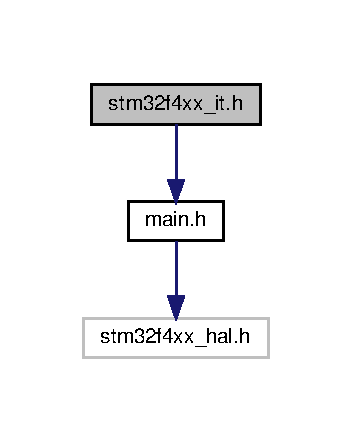
\includegraphics[width=169pt]{stm32f4xx__it_8h__incl}
\end{center}
\end{figure}
\subsection*{Functions}
\begin{DoxyCompactItemize}
\item 
void \hyperlink{stm32f4xx__it_8h_a6ad7a5e3ee69cb6db6a6b9111ba898bc}{N\+M\+I\+\_\+\+Handler} (void)
\item 
void \hyperlink{stm32f4xx__it_8h_a2bffc10d5bd4106753b7c30e86903bea}{Hard\+Fault\+\_\+\+Handler} (void)
\item 
void \hyperlink{stm32f4xx__it_8h_a3150f74512510287a942624aa9b44cc5}{Mem\+Manage\+\_\+\+Handler} (void)
\item 
void \hyperlink{stm32f4xx__it_8h_a850cefb17a977292ae5eb4cafa9976c3}{Bus\+Fault\+\_\+\+Handler} (void)
\item 
void \hyperlink{stm32f4xx__it_8h_a1d98923de2ed6b7309b66f9ba2971647}{Usage\+Fault\+\_\+\+Handler} (void)
\item 
void \hyperlink{stm32f4xx__it_8h_a3e5ddb3df0d62f2dc357e64a3f04a6ce}{S\+V\+C\+\_\+\+Handler} (void)
\item 
void \hyperlink{stm32f4xx__it_8h_adbdfb05858cc36fc520974df37ec3cb0}{Debug\+Mon\+\_\+\+Handler} (void)
\item 
void \hyperlink{stm32f4xx__it_8h_a6303e1f258cbdc1f970ce579cc015623}{Pend\+S\+V\+\_\+\+Handler} (void)
\item 
void \hyperlink{stm32f4xx__it_8h_ab5e09814056d617c521549e542639b7e}{Sys\+Tick\+\_\+\+Handler} (void)
\item 
void \hyperlink{stm32f4xx__it_8h_a17e9789a29a87d2df54f12b94dd1a0b6}{E\+X\+T\+I0\+\_\+\+I\+R\+Q\+Handler} (void)
\end{DoxyCompactItemize}


\subsection{Function Documentation}
\mbox{\Hypertarget{stm32f4xx__it_8h_a850cefb17a977292ae5eb4cafa9976c3}\label{stm32f4xx__it_8h_a850cefb17a977292ae5eb4cafa9976c3}} 
\index{stm32f4xx\+\_\+it.\+h@{stm32f4xx\+\_\+it.\+h}!Bus\+Fault\+\_\+\+Handler@{Bus\+Fault\+\_\+\+Handler}}
\index{Bus\+Fault\+\_\+\+Handler@{Bus\+Fault\+\_\+\+Handler}!stm32f4xx\+\_\+it.\+h@{stm32f4xx\+\_\+it.\+h}}
\subsubsection{\texorpdfstring{Bus\+Fault\+\_\+\+Handler()}{BusFault\_Handler()}}
{\footnotesize\ttfamily void Bus\+Fault\+\_\+\+Handler (\begin{DoxyParamCaption}\item[{void}]{ }\end{DoxyParamCaption})}

\mbox{\Hypertarget{stm32f4xx__it_8h_adbdfb05858cc36fc520974df37ec3cb0}\label{stm32f4xx__it_8h_adbdfb05858cc36fc520974df37ec3cb0}} 
\index{stm32f4xx\+\_\+it.\+h@{stm32f4xx\+\_\+it.\+h}!Debug\+Mon\+\_\+\+Handler@{Debug\+Mon\+\_\+\+Handler}}
\index{Debug\+Mon\+\_\+\+Handler@{Debug\+Mon\+\_\+\+Handler}!stm32f4xx\+\_\+it.\+h@{stm32f4xx\+\_\+it.\+h}}
\subsubsection{\texorpdfstring{Debug\+Mon\+\_\+\+Handler()}{DebugMon\_Handler()}}
{\footnotesize\ttfamily void Debug\+Mon\+\_\+\+Handler (\begin{DoxyParamCaption}\item[{void}]{ }\end{DoxyParamCaption})}

\mbox{\Hypertarget{stm32f4xx__it_8h_a17e9789a29a87d2df54f12b94dd1a0b6}\label{stm32f4xx__it_8h_a17e9789a29a87d2df54f12b94dd1a0b6}} 
\index{stm32f4xx\+\_\+it.\+h@{stm32f4xx\+\_\+it.\+h}!E\+X\+T\+I0\+\_\+\+I\+R\+Q\+Handler@{E\+X\+T\+I0\+\_\+\+I\+R\+Q\+Handler}}
\index{E\+X\+T\+I0\+\_\+\+I\+R\+Q\+Handler@{E\+X\+T\+I0\+\_\+\+I\+R\+Q\+Handler}!stm32f4xx\+\_\+it.\+h@{stm32f4xx\+\_\+it.\+h}}
\subsubsection{\texorpdfstring{E\+X\+T\+I0\+\_\+\+I\+R\+Q\+Handler()}{EXTI0\_IRQHandler()}}
{\footnotesize\ttfamily void E\+X\+T\+I0\+\_\+\+I\+R\+Q\+Handler (\begin{DoxyParamCaption}\item[{void}]{ }\end{DoxyParamCaption})}

\mbox{\Hypertarget{stm32f4xx__it_8h_a2bffc10d5bd4106753b7c30e86903bea}\label{stm32f4xx__it_8h_a2bffc10d5bd4106753b7c30e86903bea}} 
\index{stm32f4xx\+\_\+it.\+h@{stm32f4xx\+\_\+it.\+h}!Hard\+Fault\+\_\+\+Handler@{Hard\+Fault\+\_\+\+Handler}}
\index{Hard\+Fault\+\_\+\+Handler@{Hard\+Fault\+\_\+\+Handler}!stm32f4xx\+\_\+it.\+h@{stm32f4xx\+\_\+it.\+h}}
\subsubsection{\texorpdfstring{Hard\+Fault\+\_\+\+Handler()}{HardFault\_Handler()}}
{\footnotesize\ttfamily void Hard\+Fault\+\_\+\+Handler (\begin{DoxyParamCaption}\item[{void}]{ }\end{DoxyParamCaption})}

\mbox{\Hypertarget{stm32f4xx__it_8h_a3150f74512510287a942624aa9b44cc5}\label{stm32f4xx__it_8h_a3150f74512510287a942624aa9b44cc5}} 
\index{stm32f4xx\+\_\+it.\+h@{stm32f4xx\+\_\+it.\+h}!Mem\+Manage\+\_\+\+Handler@{Mem\+Manage\+\_\+\+Handler}}
\index{Mem\+Manage\+\_\+\+Handler@{Mem\+Manage\+\_\+\+Handler}!stm32f4xx\+\_\+it.\+h@{stm32f4xx\+\_\+it.\+h}}
\subsubsection{\texorpdfstring{Mem\+Manage\+\_\+\+Handler()}{MemManage\_Handler()}}
{\footnotesize\ttfamily void Mem\+Manage\+\_\+\+Handler (\begin{DoxyParamCaption}\item[{void}]{ }\end{DoxyParamCaption})}

\mbox{\Hypertarget{stm32f4xx__it_8h_a6ad7a5e3ee69cb6db6a6b9111ba898bc}\label{stm32f4xx__it_8h_a6ad7a5e3ee69cb6db6a6b9111ba898bc}} 
\index{stm32f4xx\+\_\+it.\+h@{stm32f4xx\+\_\+it.\+h}!N\+M\+I\+\_\+\+Handler@{N\+M\+I\+\_\+\+Handler}}
\index{N\+M\+I\+\_\+\+Handler@{N\+M\+I\+\_\+\+Handler}!stm32f4xx\+\_\+it.\+h@{stm32f4xx\+\_\+it.\+h}}
\subsubsection{\texorpdfstring{N\+M\+I\+\_\+\+Handler()}{NMI\_Handler()}}
{\footnotesize\ttfamily void N\+M\+I\+\_\+\+Handler (\begin{DoxyParamCaption}\item[{void}]{ }\end{DoxyParamCaption})}

\mbox{\Hypertarget{stm32f4xx__it_8h_a6303e1f258cbdc1f970ce579cc015623}\label{stm32f4xx__it_8h_a6303e1f258cbdc1f970ce579cc015623}} 
\index{stm32f4xx\+\_\+it.\+h@{stm32f4xx\+\_\+it.\+h}!Pend\+S\+V\+\_\+\+Handler@{Pend\+S\+V\+\_\+\+Handler}}
\index{Pend\+S\+V\+\_\+\+Handler@{Pend\+S\+V\+\_\+\+Handler}!stm32f4xx\+\_\+it.\+h@{stm32f4xx\+\_\+it.\+h}}
\subsubsection{\texorpdfstring{Pend\+S\+V\+\_\+\+Handler()}{PendSV\_Handler()}}
{\footnotesize\ttfamily void Pend\+S\+V\+\_\+\+Handler (\begin{DoxyParamCaption}\item[{void}]{ }\end{DoxyParamCaption})}

\mbox{\Hypertarget{stm32f4xx__it_8h_a3e5ddb3df0d62f2dc357e64a3f04a6ce}\label{stm32f4xx__it_8h_a3e5ddb3df0d62f2dc357e64a3f04a6ce}} 
\index{stm32f4xx\+\_\+it.\+h@{stm32f4xx\+\_\+it.\+h}!S\+V\+C\+\_\+\+Handler@{S\+V\+C\+\_\+\+Handler}}
\index{S\+V\+C\+\_\+\+Handler@{S\+V\+C\+\_\+\+Handler}!stm32f4xx\+\_\+it.\+h@{stm32f4xx\+\_\+it.\+h}}
\subsubsection{\texorpdfstring{S\+V\+C\+\_\+\+Handler()}{SVC\_Handler()}}
{\footnotesize\ttfamily void S\+V\+C\+\_\+\+Handler (\begin{DoxyParamCaption}\item[{void}]{ }\end{DoxyParamCaption})}

\mbox{\Hypertarget{stm32f4xx__it_8h_ab5e09814056d617c521549e542639b7e}\label{stm32f4xx__it_8h_ab5e09814056d617c521549e542639b7e}} 
\index{stm32f4xx\+\_\+it.\+h@{stm32f4xx\+\_\+it.\+h}!Sys\+Tick\+\_\+\+Handler@{Sys\+Tick\+\_\+\+Handler}}
\index{Sys\+Tick\+\_\+\+Handler@{Sys\+Tick\+\_\+\+Handler}!stm32f4xx\+\_\+it.\+h@{stm32f4xx\+\_\+it.\+h}}
\subsubsection{\texorpdfstring{Sys\+Tick\+\_\+\+Handler()}{SysTick\_Handler()}}
{\footnotesize\ttfamily void Sys\+Tick\+\_\+\+Handler (\begin{DoxyParamCaption}\item[{void}]{ }\end{DoxyParamCaption})}

\mbox{\Hypertarget{stm32f4xx__it_8h_a1d98923de2ed6b7309b66f9ba2971647}\label{stm32f4xx__it_8h_a1d98923de2ed6b7309b66f9ba2971647}} 
\index{stm32f4xx\+\_\+it.\+h@{stm32f4xx\+\_\+it.\+h}!Usage\+Fault\+\_\+\+Handler@{Usage\+Fault\+\_\+\+Handler}}
\index{Usage\+Fault\+\_\+\+Handler@{Usage\+Fault\+\_\+\+Handler}!stm32f4xx\+\_\+it.\+h@{stm32f4xx\+\_\+it.\+h}}
\subsubsection{\texorpdfstring{Usage\+Fault\+\_\+\+Handler()}{UsageFault\_Handler()}}
{\footnotesize\ttfamily void Usage\+Fault\+\_\+\+Handler (\begin{DoxyParamCaption}\item[{void}]{ }\end{DoxyParamCaption})}


%--- End generated contents ---

% Index
\backmatter
\newpage
\phantomsection
\clearemptydoublepage
\addcontentsline{toc}{chapter}{Index}
\printindex

\end{document}
